{\bfseries IRSTI 61.01.05}

{\bfseries DEVELOPMENT OF ANTIMICROBIAL PACKAGING MATERIALS FOR FOOD
PRODUCTS BASED ON COPPER NANOPARTICLES}

{\bfseries A.I.Samadun, B.R. Taussarova, Zh.S. Nabiyev., G.T.Daribayeva\\
}Almaty Technological University, Almaty, Kazakhstan

Corresponding author: abdu.93\_93@mail.ru

In the process of storage and delivery, food products are subjected to
physical changes, resulting in moisture exchange between the product and
the environment, mechanical damage, chemical processes occurring in the
product itself, as well as microbiological damage. The use of packaging
materials on the basis of polyolefins, reduce the influencing factors
leading to rapid corruption of food products. However, by their nature,
polyethylene and polypropylene films do not have antimicrobial
properties. Therefore, in order for the packaging based on them to
protect the product from microbiological damage, various technological
techniques are used for the processing of packaging, as well as the
introduction of special antimicrobial agents into the composition of the
film. The present study developed a method of synthesis of copper oxide
nanoparticles stabilized with gelatin and pectin. The synthesis was
carried out by direct chemical sedimentation. Copper chloride was used
as a precursor to the synthesis of copper oxide. Gelatin and pectin were
used as stabilizers. Gelatin and pectin were used as a stabilizer as an
environmentally friendly component of the film. In addition, consumers
are interested in innovative, economical, harmless and effective food
packaging materials.

The results showed that CuO nanoparticles, stabilized with gelatin and
pectin, have a high potential for use in food packaging -- both as a
stand-alone nanoplane and as part of other packaging materials.

{\bfseries Key words}: CuO nanoparticles, gelatin, pectin, polylactide,
antimicrobial, packaging.

{\bfseries МИКРОБҚА ҚАРСЫ ТАҒАМДЫҚ ҚАПТАМА МАТЕРИАЛДАРЫН МЫС
НАНОБӨЛШЕКТЕРІНІҢ НЕГІЗІНДЕ ӘЗІРЛЕУ}

{\bfseries А.И.Самадун, Б.Р.Таусарова, Ж.С.Набиева, Дарибаева Г.Т.}

Алматы технологиялық университеті, Алматы қ., Қазақстан,

е-mail: abdu.93\_93@mail.ru

Сақтау және сату процесінде тамақ өнімдері физикалық өзгерістерге
ұшырайды, нәтижесінде өнім мен қоршаған орта арасында ылғал алмасу,
механикалық зақымдану, өнімнің өзінде болатын химиялық процестер,
сондай-ақ микробиологиялық бүліну пайда болады. Полиолефиндерге
негізделген орау материалдарын қолдану әсер етуші факторларды азайтуға
мүмкіндік береді, бұл тағамның тез бұзылуына әкеледі. Алайда, табиғаты
бойынша полиэтилен және полипропилен пленкалары микробқа қарсы
қасиеттерге ие емес. Сондықтан, олардың негізінде қаптама өнімді
микробиологиялық бұзылудан қорғау үшін қаптаманы өңдеудің әртүрлі
технологиялық әдістері, сондай-ақ пленкаға, арнайы микробқа қарсы
агенттерге кіріспе қолданылады. Бұл зерттеуде желатин мен пектинмен
тұрақтандырылған мыс оксидінің нанобөлшектерін синтездеу әдісі жасалды.
Синтез тікелей химиялық тұндыру арқылы жүзеге асырылды. Мыс оксидін
синтездеу үшін прекурсорлар ретінде мыс хлориді қолданылды.
Тұрақтандырғыш ретінде желатин мен пектин қолданылды. Желатин мен пектин
экологиялық тұрақтандырғыш өнім ретінде қолданылды. Сонымен қатар,
тұтынушылар инновациялық, үнемді, экологиялық таза және тиімді
азық-түлік қаптама материалдарына қызығушылық танытуда\hl{.}

Нәтижелер желатин мен пектинмен тұрақтандырылған CuO нанобөлшектерінің
азық -- түлік қаптамасында-тәуелсіз нанопленка ретінде де, басқа орау
материалдарының бөлігі ретінде де пайдалану мүмкіндігі жоғары екенін
көрсетті.

{\bfseries Түйін сөздер:} CuO нанобөлшектері, желатин, пектин, полилактид,
микробқа қарсы, орау.

{\bfseries РАЗРАБОТКА АНТИМИКРОБНЫХ УПАКОВОЧНЫХ МАТЕРИАЛОВ ДЛЯ}

{\bfseries ПИЩЕВЫХ ПРОДУКТОВ НА ОСНОВЕ НАНОЧАСТИЦ МЕДИ}

{\bfseries А.И.Самадун, Б.Р.Таусарова, Ж.С.Набиева, Г.Т.Дарибаева}

Алматинский технологический университет, г. Алматы, Казахстан,

е-mail: abdu.93\_93@mail.ru

В процессе хранения и реализации пищевые продукты, подвергаются
физическим изменениям, в результате которых происходит влагообмен между
продуктом и окружающей средой, механическим повреждениям, химическим
процессам, протекающим в самом продукте, а также микробиологической
порче. Применение упаковочных материалов на основе полиолефинов,
позволяют снизить воздействующие факторы, приводящие к быстрой порче
пищевых продуктов. Однако по своей природе полиэтиленовые и
полипропиленовые пленки не обладают антимикробными свойствами. Поэтому
для того, чтобы упаковка на их основе защищала продукт от
микробиологической порчи, применяются различные технологические приемы
по обработки упаковки, а также введение в состав пленки, специальных
антимикробных агентов. В настоящем исследовании был разработан метод
синтеза наночастиц оксида меди, стабилизированных желатином и пектином.
Синтез осуществлялся путем прямого химического осаждения. В качестве
предшественников для синтеза оксида меди использовались хлорид меди. В
качестве стабилизатора использовался желатин и пектин. Как экологически
продукт в качестве стабилизатора использовался желатин и пектин. Кроме
того, потребители заинтересованы в инновационных, экономичных,
экологически чистых и эффективных упаковочных материалах для пищевых
продуктов.

Результаты показали, что наночастицы CuO, стабилизированные желатином и
пектином, обладают высоким потенциалом для использования в упаковке
пищевых продуктов -- как в качестве самостоятельной нанопленки, так и в
составе других упаковочных материалов.

{\bfseries Ключевые слова:} наночастицы CuO, желатин, пектин, полилактид,
антимикробная, упаковка.

{\bfseries Introduction.} The issue of healthy and high-quality nutrition
is global. In developing countries, this problem is linked to
underdeveloped agriculture and processing.

The high rate of urbanization has forced the population of large cities
to switch to industrial methods of food supply. Such methods require
various measures aimed at significantly extending the shelf life of
food. This constantly leads to a decrease in the nutritional value of
foodstuffs. As the population continues to grow, these challenges will
have an increasing impact on the global food distribution system,
creating imbalances between regions with varying levels of economic
development.

There are various ways to address the above challenges: agricultural
development, improved food supply chains, sustainable production and
consumption. An important factor in ensuring food security is the
development of methods to increase the shelf life of food products
without significantly reducing their quality. Such methods for extending
shelf life include the use of antimicrobial packaging. Antimicrobial
packaging is made by modifying traditional packaging to provide
protection against the growth of pathogens during food storage.

Nanoparticles are often used in the food industry to create
antibacterial films {[}1, 2{]}. Research is currently under way to
develop antimicrobial packaging materials derived from various
nanoparticles, including CuO {[}3-5{]}. Nanopackets can be applied to
food products by wrapping, grinding, brushing or spraying to provide a
selective barrier against the movement of gases, moisture and dissolved
materials, as well as protection against mechanical damage {[}6, 7{]}.
The main development is aimed at obtaining nanoparticles with subsequent
surface treatment of finished packaging materials. According to Kamran
Tahir, Dipranjan Laha, Arindam Pramanik, the activity of nanoparticles
depends on the shape and their dispersion. The stabilization of
nanoparticles is an important aspect in the design of food packaging
with nanocomposites.The bactericidal activity and migration of
nanoparticles into the product depends on the method of synthesis
{[}8{]} and determines the stability of nanoparticles in the polymer
composition of packaging materials. With high stability, migration of
CuO nanoparticles into the product will be eliminated, which guarantees
no toxicity of the packaging material. The safety of food products
during their long-term storage is influenced by a wide range of factors:
adverse influence of the external environment, processes of natural
corruption due to natural biochemical and chemical reactions,
development of microorganisms. Microbiological damage is one of the most
significant factors affecting the preservation of the quality of
foodstuffs, both of plant and animal origin.

Microbiological stability can be achieved in various ways: by adding
preservatives to the product, using special storage technologies, use of
special packaging, etc. Often many methods of preventing microbiological
damage are associated with the influence on the biochemical processes of
the life of living organisms. Along with the effects on microorganisms,
these methods can have a significant effect on a person whose body
functions according to similar biochemical patterns. Thus, the use of
preservatives reduces the quality of the product, use of special
technologies can also lead to a significant loss of nutritional value
and significantly increase the cost of products. One of the most
promising directions to increase the shelf life of foodstuffs is the use
of special packaging materials that can protect the product from
negative environmental factors, as well as reduce the rate of
microbiological damage.

The aim of this work is to development of a method for the synthesis of
CuO nanoparticles stabilised with gelatin and pectin, to study the
possibility of their using in food packaging to protect against
microbiological spoilage and increase the storage life.

{\bfseries Materials and methods.} \emph{CuO Nanoparticles Synthesis
Method.}

Reagents: Copper (II) 2-water chloride (Sigma-Aldrich Pty Ltd, Merck
KGaA branch, Darmstadt, Germany), gelatin (Segma-Aldrich Ptys Ltd, merck
KGAA subsidiary, DARMSTAD, Germany); sodium hydroxide (Shandong Zhoushun
International Trade Co., Ltd); ascorbic acid-L (SIGMA-ALDRICH PTY Ltd,
MERCK KGA A branch, darmstad, Germany) and pectin (Jiaxing Renze Import
\& Export Co., Ltd.).

CuO nanoparticles, stabilized with gelatin and pectin, were polluted by
direct chemical sedimentation. Copper chloride was used as a precursor
to CuO nanoparticles (II). Pectin and gelatin acted as a stabilizer, as
a restorative used ascorbic acid, sodium hydroxide - as a sediment.
Distilled water was used as a reaction medium.

CuO nanoparticles stabilized with gelatin and pectin were obtained by
the following procedure: 0.03 g of precursor (copper chloride), 0.03 g
of gelatine and 0.1 g of ascarbic acid, dissolved in 90 ml of reaction
medium (distilled water), a similar procedure was performed with
pectine. The resulting solution was heated to boil with constant mixing
and an additional 0.5\% solution of NaOH was added to pH-10. The sample
was mixed for 2-3 minutes, cooled to room temperature, mixed at room
temperature for 20 minutes. As a result, copper oxide nanoparticles were
produced. The phase of obtaining nanoparticles is an important component
of the work on the creation of nanocomposite packaging materials,
because it is the nanoparticle that gives the newly obtained packaging
unique properties.

For the preparation of packaging material modified by CuO nanoparticles,
polylactic film was used, which is often used in the production of
eco-packages. As a test sample, ordinary polylactic film from ECO
Prodacts Group (Astana) was taken.

As part of the development of nanoparticles preparations - visual
evaluation, microphotography of samples of CuO nanoparticles and data on
the elemental composition were obtained with the scanning electron
microscope INTEGRA TERMA and integration of probe and optical microscopy
and spectroscopy, ASM - Raman - SBOM - TERS {[}9{]}. The samples were
dried for study. The samples were prepared as follows: a two-sided
conductive carbon tape was glued to the standard toolboard. CuO powder
was applied to the conductive carbon tape. They then applied a carbon
coating about 10 nm thick. The pH was measured using the Testo 206 ph1
pH meter using a silver chloride combined electrode.

Microbiological analysis methods were used to study the antimicrobial
effectiveness of polylactide films modified with CuO nanoparticles on
bread shelf life.

The effects of polylactid films modified by CuO nanoparticles on the
quality and shelf life of bread were studied.

For the experiment they took white wheat bread produced by "Aksai nan"
(Almaty). The shelf life at the time of purchase was 3 days. In order to
study the initial parameters of the bread on the day of beginning of the
experiment, slices weighing 50±0.2g corresponding to the number of
experimental films were cut.

The bread samples were stored in the SCTC TS-1/80 SPU thermostat at 25 ±
1°C for 120 ± 3 hours of the experiment. After the time passed,
microbiological analysis was carried out. The analysis was carried out
according to GOST 10444.12-2013 Microbiology of food and animal feed.
Methods of detection and counting of yeast and mold mushrooms {[}10{]}.

{\bfseries Results and discussion.} The color of nanoparticles is an
important qualitative characteristic, because it can characterize the
size of particles and their chemical composition. The reason for the
difference in colour of colloid nanoparticles solutions is different:
the nature of the dispersion phase and the disspersion medium, particle
dispersiveness, shape and structure. All these factors affect not only
the absorption of light in the solution, but also its dispersion. Even a
slight change in the color of the solution may indicate a change in
particle size and chemical composition. Figure - 1 shows solutions of
silver nanoparticles obtained by different methods and having different
sizes.

\begin{figure}[H]
	\centering
	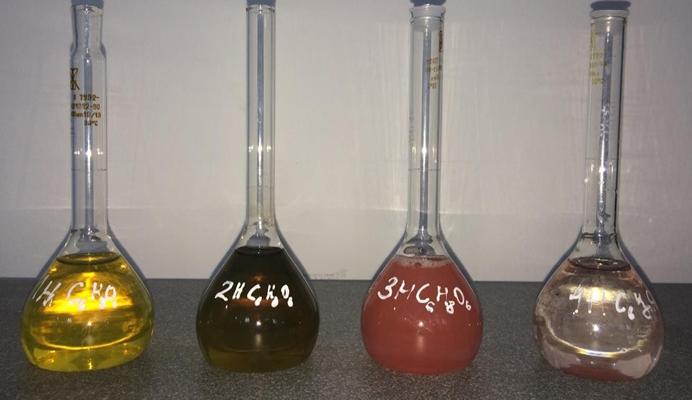
\includegraphics[width=0.8\textwidth]{assets/14}
	\caption*{}
\end{figure}

{\bfseries Fig. 1 - Appearance of copper nanoparticles solutions}

The optical spectrum of nanoparticles and nanomaterials solutions is no
less important qualitative characteristic than the color of the
solution. The method of optical spectroscopy is based on the measurement
of particle absorption of the electromagnetic radiation of the optical
range. Figure 2, 3, 4 shows the optical spectra for the colloidal
solutions studied.

{\bfseries Fig. 2 - Graph of obtained data on spectroscopic photometer
Jenway 6705}

\begin{figure}[H]
	\centering
	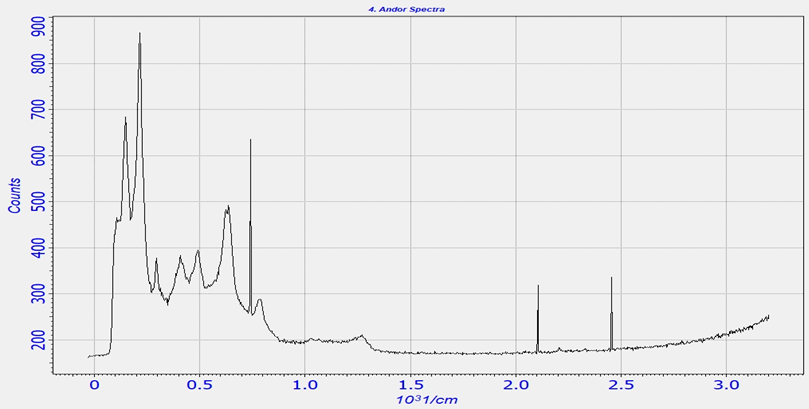
\includegraphics[width=0.8\textwidth]{assets/15}
	\caption*{}
\end{figure}

{\bfseries Fig. 3 - Optical spectrum of copper nanoparticles using gelatin
as a stabilizer in exhaust solutions}

\begin{figure}[H]
	\centering
	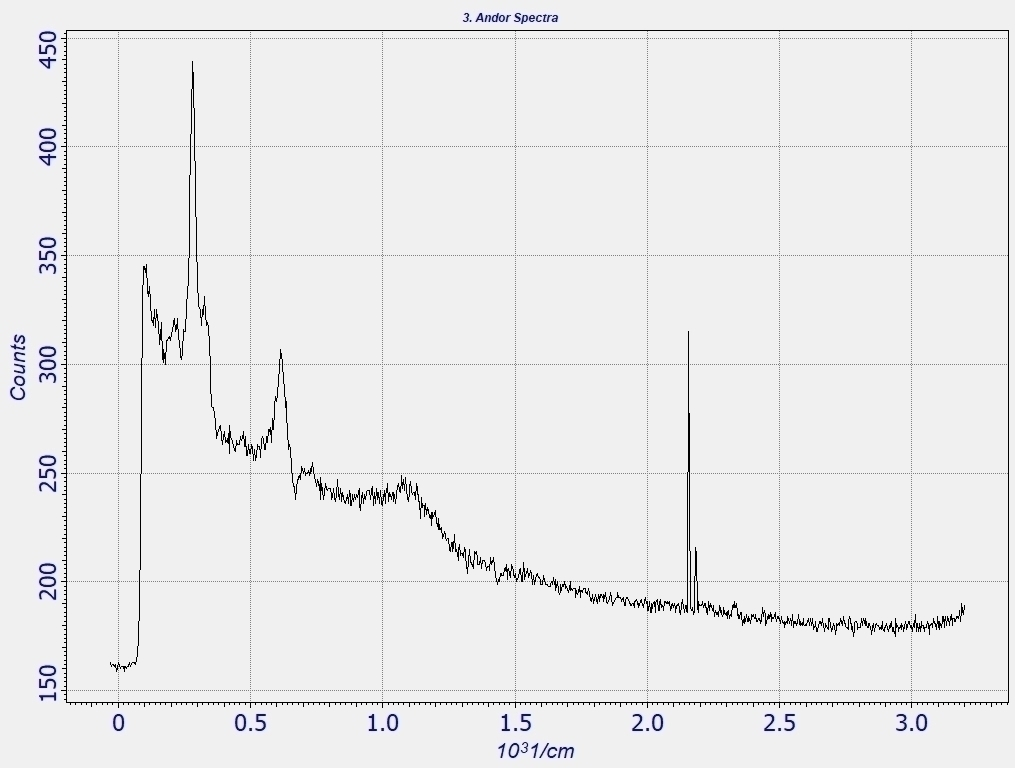
\includegraphics[width=0.8\textwidth]{assets/16}
	\caption*{}
\end{figure}

{\bfseries Fig. 4 - Optical spectrum of copper nanoparticles when pectin is
used as a stabilizer in baseline solutions}

Dispersion phase particle size is one of the most important
characteristics of colloidal solutions, determining their many
properties. In particular, the stability of the solution and its
biological properties may depend on the size of the nanoparticles
{[}11{]}. The samples showed nanoparticles with sizes ranging from 136
to 995 nm. When pectin was used as a stabiliser, and when gelatin was
used as a stabiliser, the particle sizes ranged from 62 to 313 nm.
Photos of samples made by optical and scanning electron microscope are
shown in Figures 5 - 7. Based on the results of scanning and
transmission microscopy, nanoparticles as seen in Figure 7 have
spherical shape like granules. Figure - 8 shows the surfaces of the
films before and after treatment with copper nanoparticles. In the
treated film the clusters of nanoparticles reached up to 500 nm in some
places.

% \begin{longtable}[]{@{}
%   >{\raggedright\arraybackslash}p{(\columnwidth - 2\tabcolsep) * \real{0.4896}}
%   >{\raggedright\arraybackslash}p{(\columnwidth - 2\tabcolsep) * \real{0.5104}}@{}}
% \toprule\noalign{}
% \begin{minipage}[b]{\linewidth}\raggedright
% \begin{figure}[H]
% 	\centering
% 	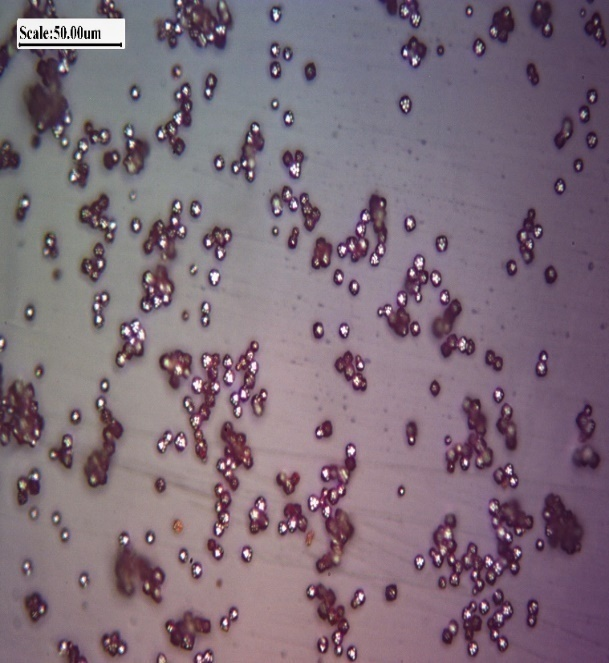
\includegraphics[width=0.8\textwidth]{assets/17}
% 	\caption*{}
% \end{figure}
% \end{minipage} & \begin{minipage}[b]{\linewidth}\raggedright
% \begin{figure}[H]
% 	\centering
% 	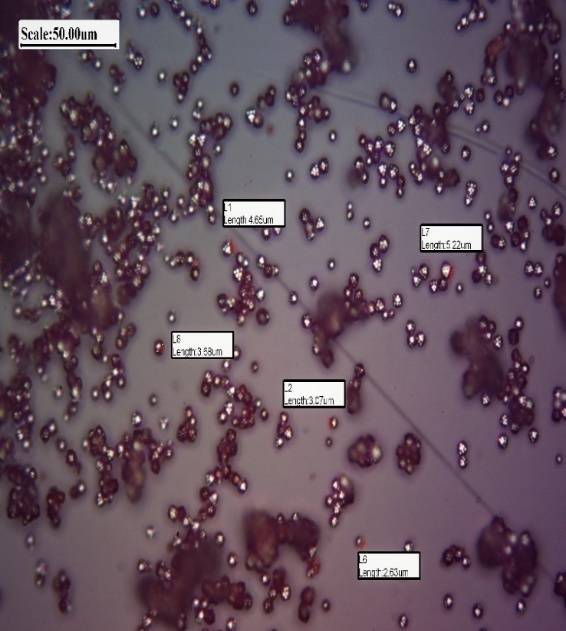
\includegraphics[width=0.8\textwidth]{assets/18}
% 	\caption*{}
% \end{figure}
% \end{minipage} \\
% \midrule\noalign{}
% \endhead
% \bottomrule\noalign{}
% \endlastfoot
% & \\
% \end{longtable}

{\bfseries Fig. 5 - Optical imaging of copper nanoparticles in the 50 μm
range}

\begin{figure}[H]
	\centering
	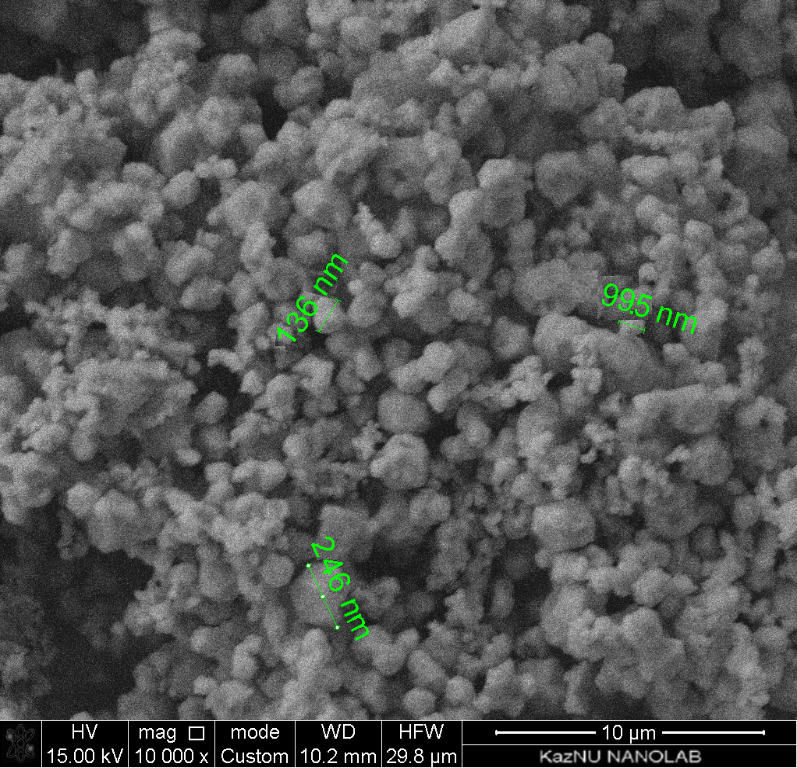
\includegraphics[width=0.8\textwidth]{assets/19}
	\caption*{}
\end{figure}

{\bfseries Fig. 6 -- Dimensions of copper nanoparticles using pectin as a
stabilizer}

\begin{figure}[H]
	\centering
	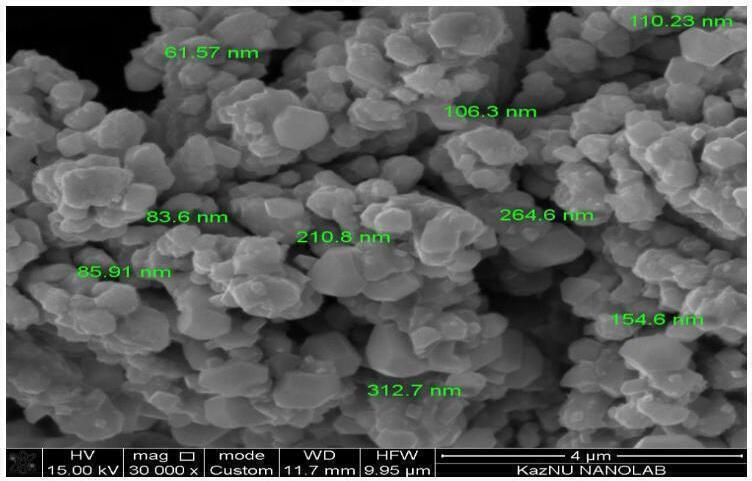
\includegraphics[width=0.8\textwidth]{assets/20}
	\caption*{}
\end{figure}

{\bfseries Fig. 7 -- Dimensions of copper nanoparticles using gelatin as a
stabilizer}

% \begin{longtable}[]{@{}
%   >{\raggedright\arraybackslash}p{(\columnwidth - 2\tabcolsep) * \real{0.4816}}
%   >{\raggedright\arraybackslash}p{(\columnwidth - 2\tabcolsep) * \real{0.5184}}@{}}
% \toprule\noalign{}
% \begin{minipage}[b]{\linewidth}\raggedright
% \begin{figure}[H]
% 	\centering
% 	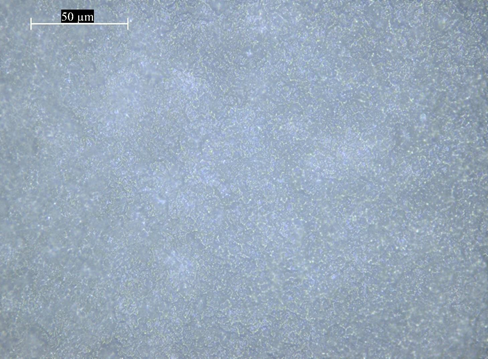
\includegraphics[width=0.8\textwidth]{assets/21}
% 	\caption*{}
% \end{figure}
% \end{minipage} & \begin{minipage}[b]{\linewidth}\raggedright
% \begin{figure}[H]
% 	\centering
% 	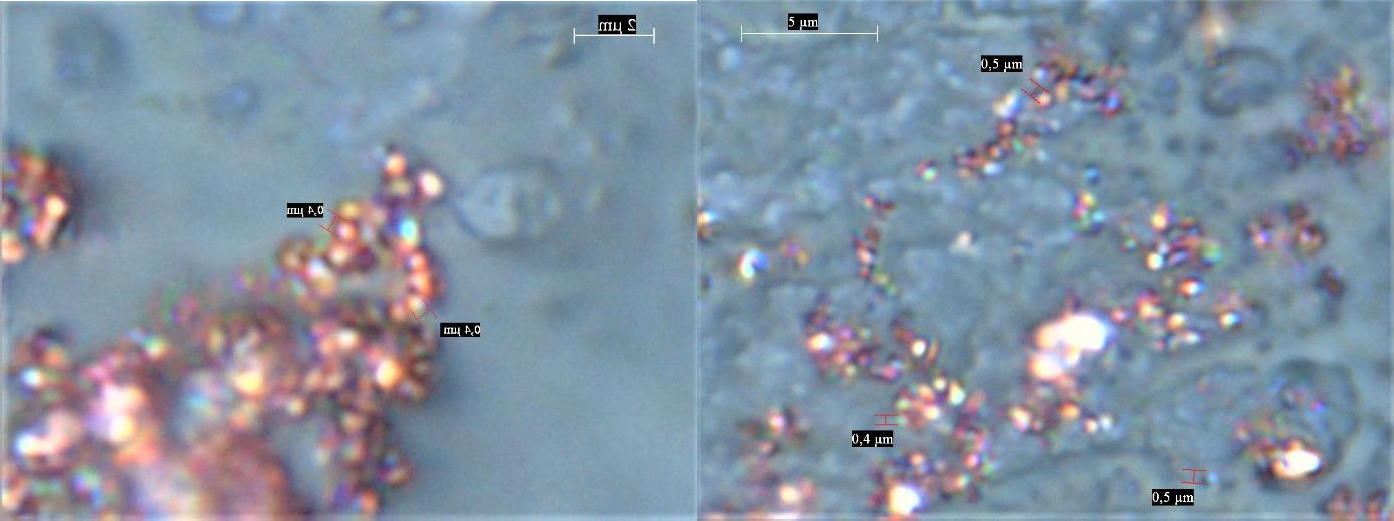
\includegraphics[width=0.8\textwidth]{assets/22}
% 	\caption*{}
% \end{figure}
% \end{minipage} \\
% \midrule\noalign{}
% \endhead
% \bottomrule\noalign{}
% \endlastfoot
% а & b \\
% \end{longtable}

{\bfseries Fig. 8 - Polylactid film samples (a) before treatment and (b)
after copper nanoparticles treatment}

As a result of the study of the basic physico-chemical characteristics
of nanoparticle solutions, it can be concluded that they differ strongly
and as a consequence different effects when they are used to create
composite packaging materials. Evaluation of the effectiveness of the
application of a product is an important part of its development
process. Since often not individual characteristics of a product are the
reason for its purchase, but the ability of the product to solve a
particular problem, it is important to determine the possibility of
solving the problem. For nanopackaging, this problem is the extension of
the shelf life of the products packaged in it. The benefits of use can
be significant if such packaging is used as effectively as possible.

In order for the packaging to be used effectively, it is necessary to
determine an extended shelf life compared to conventional packaging. It
is known that the main cause of damage is the development of various
microorganisms, so the use of packaging with antimicrobial agents is
relevant. The shelf life can be determined in different ways, depending
on the type of product.

The method of microbiological testing is most appropriate if the cause
of damage is mainly the development of microorganisms in the product. In
this case, both the total number of microorganisms (COE) can be measured
and differentiated depending on the type of micro-organism. The
advantage of this method is the ability to identify the main source
causing the damage of the product.

The effects of CuO-modified polylactid films on changes in the
microbiological purity of bread storage are further studied in Table 1
and Figure 9.

{\bfseries Table 1 - Dynamics of changes in microbiological parameters of
bread samples during storage}

\begin{longtable}[]{@{}
  >{\raggedright\arraybackslash}p{(\columnwidth - 16\tabcolsep) * \real{0.0463}}
  >{\raggedright\arraybackslash}p{(\columnwidth - 16\tabcolsep) * \real{0.3689}}
  >{\raggedright\arraybackslash}p{(\columnwidth - 16\tabcolsep) * \real{0.0845}}
  >{\raggedright\arraybackslash}p{(\columnwidth - 16\tabcolsep) * \real{0.0821}}
  >{\raggedright\arraybackslash}p{(\columnwidth - 16\tabcolsep) * \real{0.0835}}
  >{\raggedright\arraybackslash}p{(\columnwidth - 16\tabcolsep) * \real{0.0806}}
  >{\raggedright\arraybackslash}p{(\columnwidth - 16\tabcolsep) * \real{0.0791}}
  >{\raggedright\arraybackslash}p{(\columnwidth - 16\tabcolsep) * \real{0.0836}}
  >{\raggedright\arraybackslash}p{(\columnwidth - 16\tabcolsep) * \real{0.0915}}@{}}
\toprule\noalign{}
\multirow{2}{=}{\begin{minipage}[b]{\linewidth}\raggedright
№
\end{minipage}} &
\multirow{2}{=}{\begin{minipage}[b]{\linewidth}\raggedright
Sample
\end{minipage}} &
\multicolumn{7}{>{\raggedright\arraybackslash}p{(\columnwidth - 16\tabcolsep) * \real{0.5849} + 12\tabcolsep}@{}}{%
\begin{minipage}[b]{\linewidth}\raggedright
Mold index, CFU/g
\end{minipage}} \\
& & \begin{minipage}[b]{\linewidth}\raggedright
1 day
\end{minipage} & \begin{minipage}[b]{\linewidth}\raggedright
2 day
\end{minipage} & \begin{minipage}[b]{\linewidth}\raggedright
3 day
\end{minipage} & \begin{minipage}[b]{\linewidth}\raggedright
4 day
\end{minipage} & \begin{minipage}[b]{\linewidth}\raggedright
5 day
\end{minipage} & \begin{minipage}[b]{\linewidth}\raggedright
6 day
\end{minipage} & \begin{minipage}[b]{\linewidth}\raggedright
7 day
\end{minipage} \\
\midrule\noalign{}
\endhead
\bottomrule\noalign{}
\endlastfoot
1 & Bread without packaging & - & - & 1 & 3 & 5 & 8 & 17 \\
2 & Bread with a control package without processing & - & - & 1 & 2 & 3
& 4 & 10 \\
3 & Bread with processed packaging (using gelatin as a stabilizer) & - &
- & - & - & 1 & 2 & 4 \\
4 & Bread with processed packaging (using pectin as a stabilizer) & - &
- & - & - & 1 & 2 & 5 \\
\end{longtable}

{\bfseries Fig. 9 - Effect of polylactide packages treated with copper
nanoparticles on microbiological parameters}

In accordance with the results presented in Table 1 and Figure 9, films
modified with CuO nanoparticles were found to reduce mold growth and
development in experimental bread samples compared to the control bread
sample. The data obtained shows the activity of CuO nanoparticles
stabilized with gelatin and pectin, and also coincides with the data of
other authors {[}12, 13{]}, who studied the antibacterial activity of
CuO nanoparticles.

{\bfseries Conclusions.} The problem of healthy and quality nutrition,
along with the problem of adequacy of such nutrition is relevant for
modern humanity. One way of addressing this problem, as discussed in
this paper, is to keep products fresh and suitable for consumption for a
considerable period of time. Fortunately, modern technologies allow to
obtain and explore the latest materials that can be used to solve the
above-mentioned problems. As a result of the studies carried out and
presented in this paper, the following conclusions can be drawn:

1. A method of synthesis of CuO nanoparticles stabilized with gelatin
and pectin has been developed, their colloidal stability in various
dispersion media has been studied and their possibility of use in bread
packaging has been explored.

2. The results showed that the use of copper chloride as a precursor
allows to produce copper oxide (II). According to the data, copper oxide
nanoparticles stabilized by gelatin and pectin in the aquatic
environment had particles of the smallest diameter of 62 nm.

3. It has been found that CuO nanoparticles, stabilized with gelatin and
pectin, have antimicrobial activity and can be used as a material for
food nanopackets, providing an increase in the shelf life of products,
as shown in the example of bread. The high level of stability of CuO
nanoparticles stabilized with gelatin and pectin will also facilitate
their use in the creation of active food packaging materials.

4. It was found that polylactic films modified by CuO nanoparticles
inhibited mold growth and development in experimental bread samples.

5. The morphology of the surface is studied by electronic microscopy.
The result showed that when using gelatin as a stabilizer, the maximum
copper nanoparticles size was 313 nm, and when using pectin, the
particle size was 246 nm.

Thus, the results of experiments show that CuO nanoparticles, stabilized
with gelatin and pectin, have a high potential for use in food packaging
-- both as a self-propelled nanofilm and as part of other packaging
materials, and can also be laid as a basis for food interaction studies,
the environment and be useful for developers engaged in the creation of
promising packaging material.

{\bfseries References}

\begin{enumerate}
\def\labelenumi{\arabic{enumi}.}
\item
  Osovskaya I.I., Baranova A.E. Rastvory agara dlja uluchshenija
  kachestva upakovochnyh bumazhnyh materialov,
  tekstil\textquotesingle nyh i kozhanyh izdelij. // Tehnologija
  tekstil\textquotesingle\textquotesingle noj promyshlennosti, №5 (407)
  2023, pp 129-132. DOI 10.47367/0021-3497\_2023\_5\_129.
\item
  Baranchikov A.E. Sonohimicheskij sintez neorganicheskih materialov./
  A.E. Baranchikov, V.K. Ivanov, Ju.D. Tret\textquotesingle jakov.//
  Uspehi himii, 76, 147 (2007).
\item
  Galiahmetov R.N. Poluchenie nanochastic Cu2O v uslovijah
  ul\textquotesingle trazvukovoj kavitacii./ R.N. Galiahmetov, A.G.
  Mustafin, R.R. Garafutdinov, G.M. Kuznecova.// Pis\textquotesingle ma
  o materialah T.1. 2011. str 176-178.
\item
  Abdullah, A.S., Essa, F.A., Bacha, H.B. \& Omara, Z.M. Improving the
  trays solar still performance using reflectors and phase change
  material with nanoparticles // J Energy Storage 31, 101744. 2020. DOI
  10.1016/j.est.2020.101744
\item
  Magonov, S., Belikov, S., Surtchev, M., Leesment S., Malovichko I.
  High-Resolution Mapping of Quantitative Elastic Modulus of Polymers //
  Microscopy and Microanalysis. 2015. Vol. 21 (S. 3). P. 2183--2184. DOI
  10.1017/S1431927615011691.
\item
  GOST 10444.12-2013 Mikrobiologiya pishchevykh produktov i kormov dlya
  zhivotnykh. Metody vyyavleniya i podscheta kolichestva drozhzhey i
  plesnevykh gribov. - Moskva: Standartinform, 2014. - 9 s. {[}in
  Russian{]}
\item
  Gvozdenko, A.A., Siddiqui, S.A., Blinov, A.V. et al. Synthesis of CuO
  nanoparticles stabilized with gelatin for potential use in food
  packaging applications // Sci Rep. 2022. Vol 12. DOI
  10.1038/s41598-022-16878-w.
\item
  Singh, P.K., Das, A.K., Hatui, G. \& Nayak, G.C. Shape controlled
  green synthesis of CuO nanoparticles through ultrasonic assisted
  electrochemical discharge process and its application for
  supercapacitor // Mater. Chem. Phys. -2017. --P. 16--34 DOI:
  10.1016/j.matchemphys.2017.04.070.
\item
  Jana, R. et al. Improving performance of device made up of CuO
  nanoparticles synthesized by hydrothermal over the reflux method //
  Applied Surface Science. 2018. Vol. 452. P. 155--164.
  DOI:10.1016/j.apsusc.2018.04.262.
\item
  Pelegrino, M.T. et al. Effects of copper oxide nanoparticles on growth
  of lettuce (Lactuca sativa L) seedlings and possible implications of
  nitric oxide in their antioxidative defense // Environ. Monit. Assess.
  2020. Vol. 192. --P. 232--246. DOI: 10.1007/s10661-020-8188-3.
\item
  Pestovsky, Y. S. \& Martínez-Antonio, A. The use of nanoparticles and
  nanoformulations in agriculture // J. Nanosci. Nanotechnol. -2017.
  Vol. 17. P. 8699--8730 DOI: 10.1166/jnn.2017.15041.
\item
  Mousa, A. M. et al. Biosynthetic new composite material containing CuO
  nanoparticles produced by Aspergillus terreus for 47Sc separation of
  cancer theranostics application from irradiated Ca target // Appl.
  Radiat. Isot. 2020. Vol. 166, DOI: 10.1016/j.apradiso.2020.109389.
\item
  Abdullah, A. S., Essa, F. A., Bacha, H. B. \& Omara, Z. M. Improving
  the trays solar still performance using reflectors and phase change
  material with nanoparticles // Journal Energy Storage. 2020. Vol. 31.
  DOI: 10.1016/j.est.2020.101744.
\end{enumerate}

\emph{{\bfseries Information about the authors}}

Samadun A.I. - PhD student, Department of Chemistry, Chemical Technology
and Ecology, Almaty University of Technology,Almaty, Kazakhstan, е-mail:
abdu.93\_93@ mail.ru;

Taussarova B.R. - Professor of the Department of Chemistry, Chemical
Technology and Ecology, D.H.N., Almaty University of Technology, Almaty,
Kazakhstan, е-mail: birtausarova@mail.ru;

Nabiyeva Zh. S. - Director of the Scientific Research Institute of Food
Safety, PhD, Almaty University of Technology, Almaty, Kazakhstan,
е-mail: atu\_nabiyeva@mail.ru;

Daribayeva G.T. - Head of the Food Safety Test Laboratory, PhD, Almaty
University of Technology, Almaty, Kazakhstan, е-mail:
daribaeva.80@mail.ru

\emph{{\bfseries Сведение об авторах}}

Самадун А.И- докторант кафедры «Химии, химической технологии и экологии»
Алматинский технологический университет, Алматы, Казахстан, е-mail:
abdu.93\_93@ mail.ru;

Таусарова Б.Р.-профессор кафедры «Химия, химическая технология и
экология», д.х.н., Алматинский технологический университет, Алматы,
Казахстан, е-mail: birtausarova@mail.ru;

Набиева Ж.С. - Директор Научно-исследовательского института пищевой
безопасности, доктор PhD, Алматинский технологический университет,
Алматы, Казахстан, е-mail: atu\_nabiyeva@mail.ru;

Дарибаева Г.Т.- заведующая испытательной лабораторией «Пищевая
безопасность», доктор PhD, Алматинский технологический университет,
Алматы, Казахстан, е-mail: daribaeva.80@mail.ru\newpage
{\bfseries ҒТАМР 31.21.18}

{\bfseries ТӨМЕНГІ ҚЫСЫМДАҒЫ КӨМІРСУТЕКТЕРДІҢ ЭЛЕКТР ӨРІСІНДЕ}

{\bfseries ЖАНУЫН ЗЕРТТЕУ}

{\bfseries Т.Т.Машан}

Л.Н.Гумилев атындағы Еуразия ұлттық университеті, Астана, Қазақстан

togzhan-mashan@mail.ru

Бензол буының атомдық қатынасы C/O = 1,0 болатын оттегі ортасында
жүйесіндегі P = 40 Торр қысымда, көлемі 10\% аргон қосылғанда жануы
кезінде күйе түзілу процесіне, күйе бөлшектерінің шығымы мен құрылымына
және фуллерен шығымына U = 0,5...20 кВ кернеу диапазонындағы әртүрлі
полярлы электр өрісінің әсері зерттелді. Алынған нәтижелерді талдау
белгілі бір жағдайларда сыртқы электр өрісінің әсері электр өрісін
қолданбаған шығымдылықпен салыстырғанда күйе шығымын (10\%-ға дейін)
арттыруы мүмкін екенін көрсетті. Күйе бөлшектері U≥20 кВ кернеуде теріс
полярлық үшін тепе-теңдік аймағында дислокациямен қалыпты таралу заңымен
көбірек сипатталатыны анықталды. Электр өрісі, жалпы алғанда, өріс
әсерінсіз алынған бөлшектердің орташа өлшемімен салыстырғанда, күйе
бөлшектерінің орташа мөлшерінің ұлғаюына ықпал етеді. Кернеу өзгерген
кезде күйе пакетінің L\textsubscript{a} диаметрінің ұзындығы оның
L\textsubscript{c} биіктігінен жоғарырақ өзгеретіні анықталды.
ИҚ-спектроскопия көмегімен күйе сығындыларында C\textsubscript{60},
C\textsubscript{70} фуллерендер және ПЦАК анықталды. Аномальды жарқырау
разряды аймағында жалынға электр өрісі әсер еткенде фуллерендер шығымы
айтарлықтай арта бастайтыны анықталды (α≥13\%). Күйе үлгілерінің құрғақ
сығындыларының рентгендік фотограммасын талдау С\textsubscript{60} және
С\textsubscript{70} фуллерендеріне тән шыңдардың болуын көрсетті. Шыңдар
фуллерендердің келесі кристалдық фазаларына сәйкес келеді: орторомбты,
кубтық және алтыбұрышты (C\textsubscript{70} тек алтыбұрышты).

{\bfseries Түйін сөздер:} күйе түзілу, фуллерен, экстракция, электр өрісі,
төмен температура, ПЦАК.

{\bfseries ИССЛЕДОВАНИЕ ГОРЕНИЯ УГЛЕВОДОРОДОВ ПРИ НИЗКОМ ДАВЛЕНИИ В
ЭЛЕКТРИЧЕСКОМ ПОЛЕ}

{\bfseries Т.Т. Машан}

Евразийский национальный университет им. Л.Н. Гумилева, Астана,
Казахстан,

е-mail: togzhan-mashan@mail.ru

Исследовано влияние постоянного электрического поля различной полярности
на процесс сажеобразования, выход и структуру сажевых частиц, на выход
фуллеренов в диапазоне напряжений U=0,5...20 кВ при сжигании паров
бензола в среде кислорода при атомном соотношении С/О=1,0 с добавлением
10 \% аргона по объему, при давлении в системе Р=40 Торр. Анализ
полученных результатов показал, что воздействие внешнего электрического
поля при определенных условиях может увеличить выход сажи (до 10 \%) по
сравнению с выходом без применения электрического поля. Установлено, что
для частиц сажи наиболее характерен нормальный закон распределения с
дислокацией в зоне равновесия для отрицательной полярности при
напряжении U≥20 кВ. Электрическое поле, в целом, способствует росту
среднего размера частиц сажи по сравнению со средним размером частиц,
полученных без воздействия поля. Установлено, что длина диаметра
сажевого пакета L\textsubscript{a} подвержена большему изменению в
сторону увеличения, чем его высота L\textsubscript{с}, при изменении
напряжения. Методом ИК-спектроскопии в экстрактах сажи идентифицированы
фуллерены С\textsubscript{60}, С\textsubscript{70} и ПЦАУ. Установлено,
что выход фуллеренов значительно начинает расти (α≥13\%) при наложении
на пламя электрического поля в области аномального тлеющего разряда.
Анализ рентгеновской фотограммы сухих экстрактов образцов сажи показал
наличие пиков, характерных для фуллеренов С\textsubscript{60} и
С\textsubscript{70}. Пики соответствуют следующим кристаллическим фазам
фуллеренов: орторомбической, кубической и гексагональной
(C\textsubscript{70} только гексагональная).

{\bfseries Ключевые слова:} сажеобразование, фуллерен, экстракция,
электрическое поле, низкая температура, ПЦАУ.

{\bfseries STUDY OF HYDROCARBON COMBUSTION AT LOW PRESSURE IN}

{\bfseries AN ELECTRIC FIELD}

{\bfseries T.T. Mashan}

L.N. Gumilyov Eurasian National University{\bfseries ,} Astana, Kazakhstan,

е-mail: togzhan-mashan@mail.ru

Influence of a constant electric field of different polarity on
sootformation process, yield and structure of soot particles, on yield
of fullerenes in a range of pressure U=0.5 \ldots{} 20 kV at burning of
benzene vapours in the environment of oxygen at atomic ratio С/О=1.0
with addition of 10 \% of argon on volume, at pressure in system Р=40
Torr is investigated. The analysis of obtained results has shown, that
influence of external electric field under certain conditions can
increase yield of soot (up to 10 \%) in comparison with yield without
applying electric field. It is found that for soot particles most
typical the normal law of distribution with dislocation in the zone of
equilibrium for negative polarity at pressure U≥20 кV. The electric
field, as a whole, promotes growth of the average size soot particles in
comparison with the average size of particles received without field
influence. It is established, that the length of diameter soot package
L\textsubscript{a} is subject to greater change aside increases, than
its height L\textsubscript{с}, at voltage change. Fullerenes
C\textsubscript{60}, С\textsubscript{70} and PAH are identified in
extracts of soot by the method of IR-spectroscopy. It is established,
that yield of fullerenes significantly starts to grow (α≥13\%) at
applying on flame of electric field in the abnormal glow discharge area.
The analysis of X-ray photogram of soot samples dry extracts showed
presence of peaks, characteristic for fullerenes C\textsubscript{60} and
C\textsubscript{70}. Peaks correspond to following crystal phases of
fullerenes: orthorhombic, cubic and hexagonal (C\textsubscript{70} only
hexagonal).

{\bfseries Keywords}: Sootformation, fullerenes, extraction, electrical
field, low pressure, РАН.

{\bfseries Кіріспе.} Күйенің ауылшаруашылығының көптеген салаларында
кеңінен пайдаланылуына байланысты күйе түзілу мәселелері қазіргі заманда
маңыздылыққа ие болып отыр. Қоршаған орта жағдайларында жоғары
тұрақтылық пен ұзақ сақталуға қабылеттілігімен ерекшеленетін күйе
бөлшектері, сонымен қатар, полициклды ароматты көмірсутектер (ПЦАК) де
атмосфераны ластайтын көмірсутек майларын жағу өнімдерінің компоненттері
болып табылатындықтан, экология мәселесі де шиеленісе түсуде. Күйе мен
канцерогенді полициклды ароматты көмірсутектердің шығымын төмендету үшін
қажетті шараларды енгізу, олардың түзілу процесстерін тереңдете
зерттеуді талап етеді.

Жану процесі оң және теріс зарядты иондардың, сондай-ақ, электрондардың
пайда болуымен көрінетін физикалық әсерлермен бірге жүреді {[}1{]}. Күйе
жалындарының құрылымын зерттеу күйе пайда болғанға дейін және оның пайда
болу кезінде болатын химиялық және физикалық процестер туралы құнды
мәліметтер береді, атап айтқанда, қоршаған ортаны бензин мен дизельді
қозғалтқыштардың толық жанбаған өнімдерінен қорғау мәселесіне байланысты
қызығушылық тудырады.

Күйе түзілуін зерттеудің тағы бір маңызды аспектісі - электр өрісінің
жалын құрылымына әсері. Жану процестеріне электр өрісінің әсерін зерттеу
нәтижесінде төмен кернеулі электр өрісін қолдану жану кинетикасына
айтарлықтай әсер ететіні анықталды және көмірсутекті жалындардағы күйе
түзілу процесі көбінесе жалындағы оң зарядталған күйе бөлшегімен
анықталатыны көрсетілді {[}2, 3{]}.

Сыртқы электр өрісінің қолданылуы жалында болатын барлық процестерге:
күйе бөлшектерінің пайда болу процесіне, олардың өсуіне, сонымен қатар,
шөгуіне әсер ететіні белгілі. Күйе бөлшектерінің пайда болуы процесіне
келетін болсақ, иондық теория бар, оған сәйкес
C\textsubscript{n}H\textsubscript{n}\textsuperscript{+} типті иондар
күйе бөлшектерінің өсуінің белсенді орталықтары болып табылады {[}4{]}.
Бөлшектердің мөлшері мен массасы жану аймағында болу уақытымен
анықталады және оны электр өрісін қолдану арқылы өзгертуге болады,
өйткені барлық бөлшектер процестің ең ерте кезеңдерінде зарядтанады.

Атмосфералық қысымда метанның оттегі жалынындағы күйе бөлшектерінің
мөлшеріне және шығым процесіне 0,1-ден 2,2 кВ-қа дейінгі диапазондағы
тұрақты электр өрісінің әсерін анықтау бойынша зерттеулер жүргізілді
{[}5{]}. Полярлығына тәуелсіз электр өрісін қолданғанда, күйе
бөлшектерінің массалық шығымы азайып, олардың мөлшері кішірейіп, күйе
бөлшектерінің құрамы біртекті болатыны анықталды.

Электр өрісінің беттік жануға әсері {[}6{]} сипатталған. Тәжірибелерде
табиғи газ бен ауаның жанғыш қоспасы қолданылған. Қоспаның жануы
матрицаның бетінен жоғары аймақта жүреді. Тәжірибелерде қызықты әсер
анықталған. Электродқа жоғары оң потенциалды қолданғанда, электрод
астындағы аймақта беттік жанудың «бұғатталуы» байқалады. Жарық матрицада
қара дақ пайда болады. Кернеу азайған сайын қараңғы аймақтың көлемі
кішірейеді. Беттік жануды «бұғаттау» әсері екі себепке байланысты болуы
мүмкін: жалын шебінің беттік аймақтан жойылуы немесе иондық желдің қарсы
қысымы әсерінен ағынға жергілікті газ-динамикалық кедергінің жоғарылауы
салдарынан жергілікті жану қуатының төмендеуі.

Тұрақты және импульстік-периодты электр өрісінің пропан-ауа қоспасының
жануына әсері {[}7{]} жұмыста зерттелген. Тәжірибе көрсеткендей, кернеу
берілгенде иондық желдің пайда болуынан жалын пішіні өзгереді.
Ламинарлық жану режимінде тұрақты кернеу 3,4 кВ-қа өзгергенде жалынның
таралу жылдамдығы шамамен 20\%-ға артады. Турбулентті режим үшін бұл
жылдамдық шамамен 30\%-ға артады. Айнымалы кернеу электродына 1 кВ
бергенде, 4 мс ұзақтықтағы импульстарды беру жиілігі 150 Гц-тен бастап
өзгертсе жиіліктің артуы тұрақты өрісті қолданғандағыдай жалынның таралу
жылдамдығының айтарлықтай артуына алып келді. Тәжірибелерде, сонымен
қатар, ламинарлы режимнен турбулентті жану режиміне көшу кезінде
жалынның тұрақтылығына тұрақты электр өрісінің әсері анықталды.

Көмірсутекті жалынға әсер ететін электр өрісі заряд тасымалдаушыларға
электр денесінің күші әсерінен иондық жел тудырады. Иондық жел күйе
шығаруға, жалынның таралу жылдамдығына және жалын тұрақтылығына әсер
ететіні көрсетілген, бірақ иондық желдің егжей-тегжейлі әрекеті және
оның жалынға әсері әлі анық емес. Екі параллель электродтың арасына
орнатылған сопло арқылы өтетін араласпаған және алдын ала араластырылған
жалындарға тұрақты және айнымалы электр өрістерін берген кездегі жалын
мен иондық желдің динамикалық әрекеті зерттелген. Ион желі анодқа да,
катодқа да қарай соғатыны тіркелген және жалын түріне (араластырылмаған
немесе алдын ала араласқан) немесе электр өрісінің көзіне (тұрақты және
айнымалы тоқ) тәуелді емес {[}8{]}.

Маңызды технологиялық шикізат болғандықтан күйе өнеркәсіптік ауқымда
әртүрлі тәсілдермен өндіріледі. Негізінен \textasciitilde1700 К
температурада сұйық және газ тәрізді көмірсутектерді жеткіліксіз оттекте
жағу, содан кейін ыдырау өнімдерін жылдам салқындату арқылы термиялық
ыдырау әдісі қолданылады. Мұндай күйе материалы жеке тұйықталған
бөлшектерден тұрады, мұнда диаметрі ондаған және жүздеген Å болатын
сфералық глобулалар біріншілік болып табылады, олар бір-бірімен химиялық
байланысып, сызықтық тармақталу тізбектері спиральдар, кластерлер және
т.б. сияқты агрегаттарға біріктіріліп, екінші реттік құрылым түзуге
қабілетті {[} 9{]}.

Күйе түзілу механизмі туралы көптеген теориялар мен идеялар бар, күйе
түзілу процесіне келесі аралық өнімдер қатысады: С, С\textsubscript{2},
СН, С\textsubscript{2}Н, СН\textsubscript{2},
С\textsubscript{3}Н\textsubscript{4},
С\textsubscript{4}Н\textsubscript{3}; полиацетилендер
C\textsubscript{4}H\textsubscript{2},
C\textsubscript{6}H\textsubscript{2},
C\textsubscript{10}H\textsubscript{2}; полициклді ароматты
көмірсутектер, сондай-ақ, 1,3-бутадиен немесе винилацетилен сияқты
қосарланған байланыстары бар молекулалар {[}10, 11{]}. Көмірсутекті
газдарды жағу кезінде көміртекті наноқұрылым -- фуллерендер алу
мүмкіндігі анықталған {[}12{]}.

Бұл жұмыста төмен қысымда 0,5-тен 20 кВ-қа дейінгі кернеу диапазонындағы
күйе бөлшектерінің құрылымы мен күйе түзілу процесіне электр өрісінің
әсері зерттелген және түзілген күйе құрамында фуллерендердің болатыны
дәлелденді.

{\bfseries Материалдар мен әдістер.} Зерттеулер бензол буының оттегімен C/O
= 1,0 атомдық қатынасында 10\% аргонды қосу арқылы жануы 40 Торр қысымда
жүргізілді.

Бензол сұйықтыққа арналған шприц тәріздес мөлшерлегіш арқылы 1 мл/мин
мөлшерінде реакторға енгізілді, бұл көлемдік бу шығынының
Q\textsubscript{1} = 250 см\textsuperscript{3}/мин мөлшерін қамтамасыз
етті. Оттегі мен аргон ∆Р = 5 кгс/см\textsuperscript{2} қысымда
редукторлар арқылы берілді және капиллярлық шығын өлшегіштермен
бақыланды. Құрылғының схемасы 1-суретте көрсетілген.

\begin{figure}[H]
	\centering
	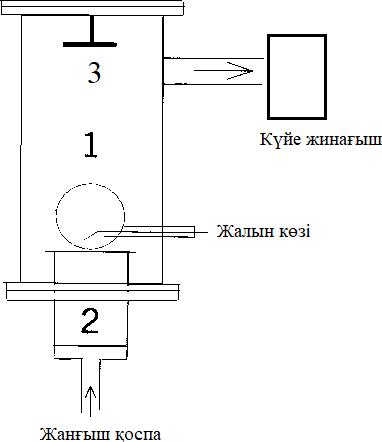
\includegraphics[width=0.8\textwidth]{assets/23}
	\caption*{}
\end{figure}

{\bfseries 1-сурет Төменгі қысымда күйе алу жандырғысының схемамы}

Жанғыш қоспаны дайындау келесі реттілікпен өтті. Сұйық бензол
мөлшерлегіш арқылы буландырғышқа енгізілді, алдын ала таңдалған
температуралық режим оның бірден дерлік булануын қамтамасыз етті.
Түзілген бензол булары буландырғышқа түсетін оттегі мен аргон
молекулаларымен араласып, содан кейін қоспа сифон тәрізді буқыздырғыш
буферлік ыдысқа түсті. Жақсы араластырылу үшін жанғыш қоспаны буферлік
резервуарға ұшы дәнекерленген перфорацияланған түтік арқылы өткізді.
Бу-газ жанғыш қоспасының соңғы дайындығы тікелей инертті материалдан
жасалған шарлармен толтырылған жандырғыда аяқталды. Бензол буларының
конденсациясын болдырмау үшін жанғыш қоспаны беру жолы қыздырылады.
Буферлік ыдыста пайда болған бу-газ қоспасының P\textsubscript{арт} = 13
кПа шегіндегі артық қысымы жанғыш қоспаның жандырғыға біркелкі берілуін
қамтамасыз етеді. Цилиндрлік жандырғының перфорацияланған
тұрақтандырғышынан жанғыш қоспаның шығу жылдамдығы V = 18,38 см/с болды.
Осы жағдайда жалындағы максималды температура T = 1200 К және жалын шебі
жандырғыдан δ = 0,5-0,8 см ажырайтын тұрақты жану туындады. Бір
тәжірибенің ұзақтығы τ = 20 мин. Жану циклі аяқталғаннан кейін кварц
реакторы мен күйе жинағыштың қабырғаларынан күйе жиналып, өлшеніп,
электронды микроскопта және ДРОН -3M дифрактометрінде
(Cu\textsubscript{α} -- сәулелену) зерттелді.

Электродтар арақашықтығы L = 18 см болатын ине-жазықтық электрод жүйесі
кварц реакторында (1) орналастырылған. Жазық электрод - сумен
салқындатылатын жандырғы (2). Ине тәрізді электродқа (3) оң немесе теріс
полярлық 0,5-тен 20 кВ-қа дейінгі диапазондағы тұрақты жоғары вольтты
кернеу берілді. Нәтижесінде жалын аймағын да, жану өнімдерінің аймағын
да қамтитын бойлық электр өрісі пайда болды.

Электр өрісі қолданылған кезде электрондардан, оң және теріс иондардан
тұратын кеңістік зарядын туындататын теріс немесе оң тәж разряды пайда
болды. Кеңістіктік заряд жалын шебіне орналастырылды және жану процесіне
тікелей әсер етті.

{\bfseries Нәтижелер} {\bfseries мен талқылау.} Әртүрлі жағдайларда алынған
күйе 72 сағат бойы бензолда суық экстракция әдісімен экстракцияланды.
Сығынды қаныққан қою қызыл түске ие болды, ол ПЦАК пен фуллерендердің
болуына сәйкес келеді. Содан кейін сығынды ИҚ-Фурье спектрометрі
көмегімен талданды. Күйе сығындысы қабықшасының ИҚ жұтылу спектрі 3050
см\textsuperscript{-1}-де жұтылу ароматты сақиналардың С-Н
байланыстарына сәйкес екенін көрсетті. 2960, 2870, 1470, 1390
см\textsuperscript{-1} жұтылу жолақтары CH\textsubscript{2} және
CH\textsubscript{3} функционалдық топтарындағы C-H тербелістік
байланыстарына сәйкес келеді. 1600 см\textsuperscript{-1} спектрі
ароматты сақинаның С=С байланыстарына сәйкес келеді. Сондай-ақ, С=О және
С-С байланыстарына сәйкес келетін жұту жолақтары бар. Спектрлерден
фуллерендердің болатыны да байқалады. Электр өрісін беру арқылы алынған
күйе сығындыларының спектрлері 2-суретте, а, б, в көрсетілген: а) U=1
кВ, б) U=2,0 кВ, в) U=20,0 кВ.

\begin{figure}[H]
	\centering
	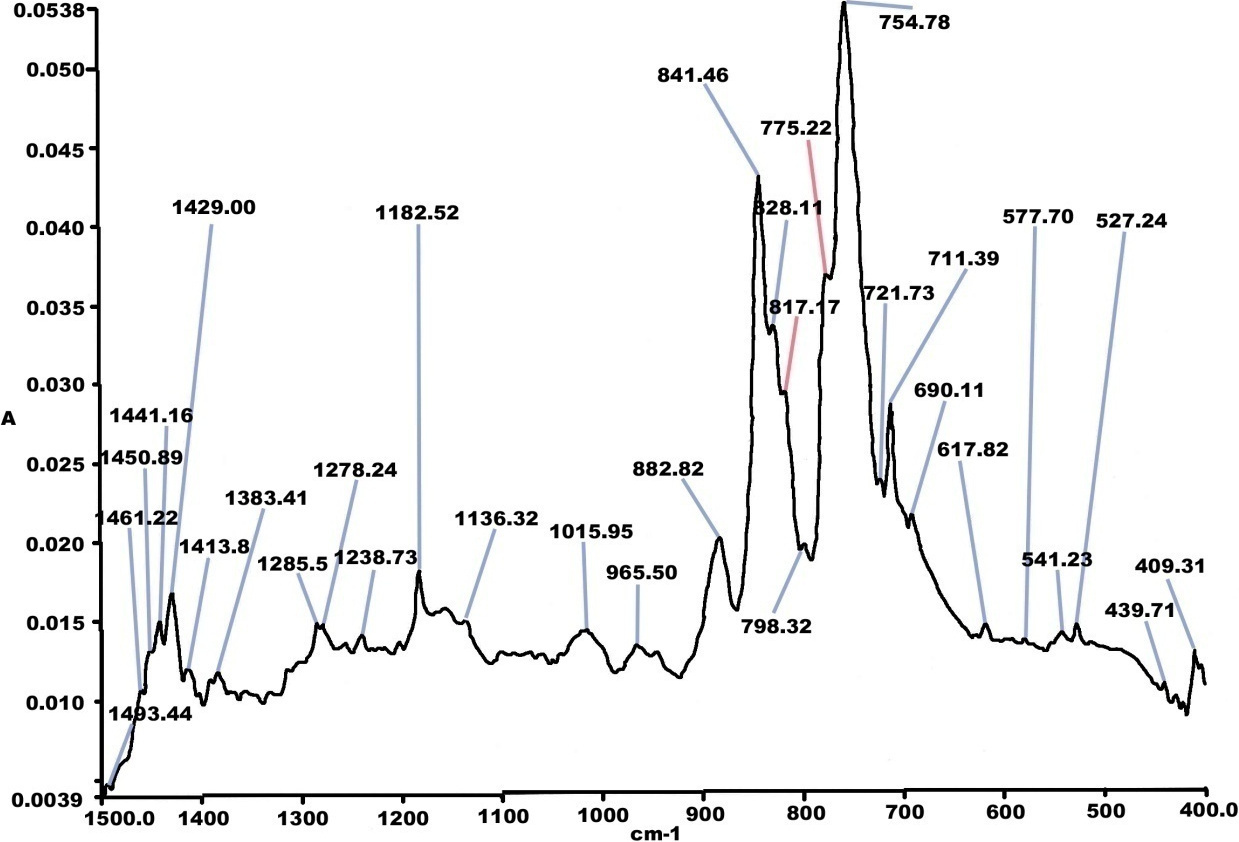
\includegraphics[width=0.8\textwidth]{assets/24}
	\caption*{}
\end{figure}

\emph{а) U=1,0 кВ,}

\begin{figure}[H]
	\centering
	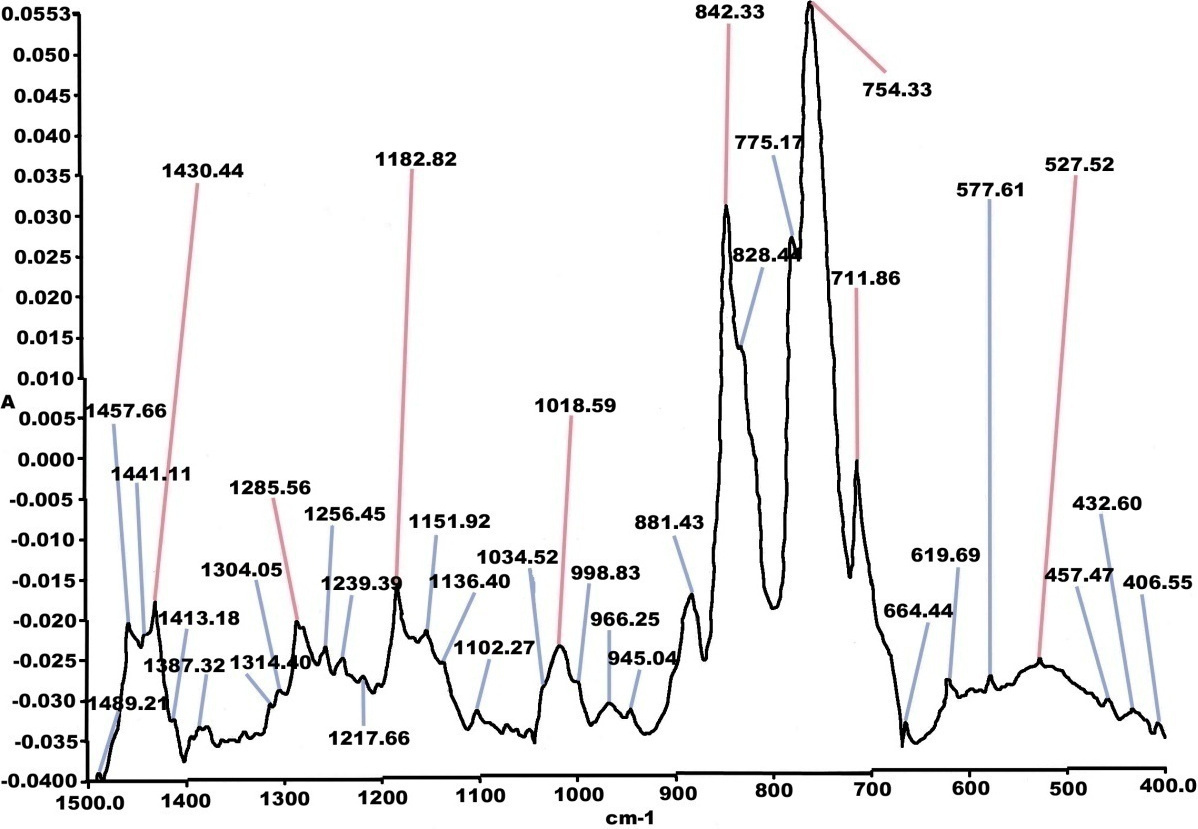
\includegraphics[width=0.8\textwidth]{assets/25}
	\caption*{}
\end{figure}

\emph{б) U=2,0 кВ}

\begin{figure}[H]
	\centering
	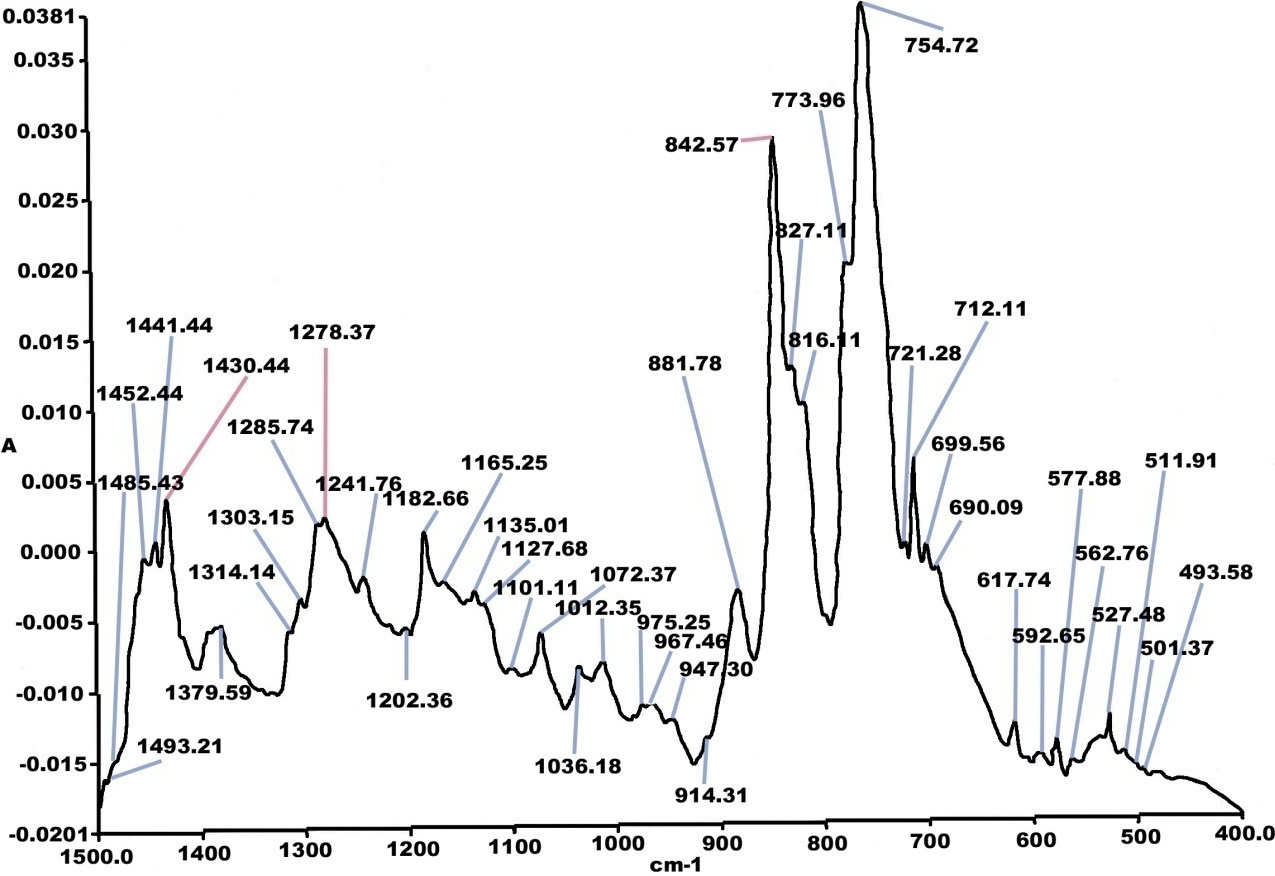
\includegraphics[width=0.8\textwidth]{assets/26}
	\caption*{}
\end{figure}

в) U=20,0 кВ

{\bfseries 2-сурет. Күйе сығындыларының ИҚ спектрлері}

1-кестеде ПЦАК және С\textsubscript{60} және С\textsubscript{70}
фуллерендеріне сәйкес тәжірибелік жолмен алынған және эталондық ИҚ
спектрлері көрсетілген.

{\bfseries 1-кесте. ПЦАК және фуллерендердің тәжірибелік және эталондық
спектрлерін салыстыру}

\begin{longtable}[]{@{}
  >{\raggedright\arraybackslash}p{(\columnwidth - 4\tabcolsep) * \real{0.2064}}
  >{\raggedright\arraybackslash}p{(\columnwidth - 4\tabcolsep) * \real{0.4286}}
  >{\raggedright\arraybackslash}p{(\columnwidth - 4\tabcolsep) * \real{0.3651}}@{}}
\toprule\noalign{}
\endhead
\bottomrule\noalign{}
\endlastfoot
Фуллерендер & Тәжірибелік , λ, см\textsuperscript{-1} & Эталон, λ
см\textsuperscript{-1} \\
С\textsubscript{60} & 528, 578, 1183, 1429 & 528, 577, 1183, 1429 \\
С\textsubscript{70} & 457, 538, 563, 578, 679, 798, 1136, 1414, 1430,
1460 & 458, 535, 565, 578, 642, 674, 795, 1134, 1414, 1430, 1460. \\
\multicolumn{3}{@{}>{\raggedright\arraybackslash}p{(\columnwidth - 4\tabcolsep) * \real{1.0000} + 4\tabcolsep}@{}}{%
ПЦАК} \\
Пирен & 711, 755, 842, 1183 & 710, 750, 840, 1190 \\
Флуорантен & 618, 755, 775, 827 & 615, 750, 775, 825 \\
Коронен & 543, 842, 1314 & 545, 850, 1313 \\
Антантрен & 690, 775, 880 & 690, 762, 877 \\
1,12-бензперилен & 755, 775, 817, 842 & 645, 750, 765, 817, 845 \\
\end{longtable}

Әртүрлі электр өрістерінде алынған күйе үлгілері үшін рентгендік
дифракциялық сипаттамалары және күйенің массалық шығымы анықталды
(2-кесте). Рентген сәулелерінің дифракциялық үлгілері бойынша үлгі
бөлшектері түзілетін күйе пакетінің құрылымын сипаттайтын
L\textsubscript{a}, L\textsubscript{c}, d\textsubscript{002} когерентті
шашырау аймағының мәндері есептелді. Мұндағы L\textsubscript{a} -- күйе
пакетінің диаметрінің ұзындығы, L\textsubscript{c} -- биіктігі,
d\textsubscript{002} -- күйе пакетіндегі екі қабат арасындағы қашықтық.

{\bfseries 2-кесте. Электр өрісін қолданған кездегі рентген құрылымдық
сипаттамалар және күйе шығымы}

% \begin{longtable}[]{@{}
%   >{\raggedright\arraybackslash}p{(\columnwidth - 12\tabcolsep) * \real{0.1045}}
%   >{\raggedright\arraybackslash}p{(\columnwidth - 12\tabcolsep) * \real{0.1194}}
%   >{\raggedright\arraybackslash}p{(\columnwidth - 12\tabcolsep) * \real{0.2239}}
%   >{\raggedright\arraybackslash}p{(\columnwidth - 12\tabcolsep) * \real{0.1194}}
%   >{\raggedright\arraybackslash}p{(\columnwidth - 12\tabcolsep) * \real{0.1492}}
%   >{\raggedright\arraybackslash}p{(\columnwidth - 12\tabcolsep) * \real{0.1641}}
%   >{\raggedright\arraybackslash}p{(\columnwidth - 12\tabcolsep) * \real{0.1194}}@{}}
% \toprule\noalign{}
% \endhead
% \bottomrule\noalign{}
% \endlastfoot
% № & U, кВ & Өрістердің орналасуы & L\textsubscript{a}, Å &
% L\textsubscript{c}, Å & d\textsubscript{002}, Å & m\textsubscript{к,}
% г \\
% 1. & Өріссіз & - & 38,13 & 9,42 & 3,71 & 0,5839 \\
% 2. & 0,5 & ± & 31,64 & 8,16 & 3,71 & 0,4633 \\
% 3. & 1,1 & ± & 65,71 & 10,0 & 3,71 & 0,4848 \\
% 4. & 2,05 & ± & 65,7 & 11,41 & 3,71 & 0,5270 \\
% 5. & 3,05 & ± & 57,5 & 11,86 & 3,70 & 0,3784 \\
% 6. & 10 & ± & 57,5 & 11,86 & 3,70 & 0,3322 \\
% 7. & 20 & ± & 57,5 & 11,4 & 3,87 & 0,3631 \\
% 8. & 0,5 & \begin{figure}[H]
% 	\centering
% 	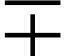
\includegraphics[width=0.8\textwidth]{assets/27}
% 	\caption*{}
% \end{figure} & 52,33 & 8,66 & 3,71 &
% 0,4632 \\
% 9. & 1,1 & \begin{figure}[H]
% 	\centering
% 	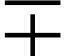
\includegraphics[width=0.8\textwidth]{assets/28}
% 	\caption*{}
% \end{figure} & 52,07 & 9,58 & 3,69 &
% 0,6216 \\
% 10. & 2,05 & \begin{figure}[H]
% 	\centering
% 	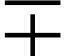
\includegraphics[width=0.8\textwidth]{assets/28}
% 	\caption*{}
% \end{figure} & 65,7 & 12,71 & 3,70 &
% 0,4695 \\
% 11. & 3,05 & \begin{figure}[H]
% 	\centering
% 	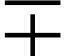
\includegraphics[width=0.8\textwidth]{assets/28}
% 	\caption*{}
% \end{figure} & 49,73 & 13,09 & 3,65
% & 0,3752 \\
% 12. & 10 & \begin{figure}[H]
% 	\centering
% 	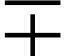
\includegraphics[width=0.8\textwidth]{assets/28}
% 	\caption*{}
% \end{figure} & 49,73 & 12,0 & 3,78 &
% 0,3167 \\
% 13. & 20 & \begin{figure}[H]
% 	\centering
% 	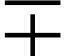
\includegraphics[width=0.8\textwidth]{assets/28}
% 	\caption*{}
% \end{figure} & 40,0 & 9,67 & 3,70 &
% 0,4070 \\
% \end{longtable}

Кестеден көрініп тұрғандай, полярлықты өзгерту күйе бөлшектерінің шығымы
мен мөлшеріне қатты әсер етеді.

Күйе үлгілерінің микроэлектрондық кескіндері алынды, 2-сурет. 0,5-тен 2
кВ-қа дейінгі электр өрісін қолданғанда, алынған күйе үлгілерінің
өлшемдері 261 Å-ден 334 Å-ге дейін өзгерді.

% \begin{longtable}[]{@{}
%   >{\raggedright\arraybackslash}p{(\columnwidth - 4\tabcolsep) * \real{0.3330}}
%   >{\raggedright\arraybackslash}p{(\columnwidth - 4\tabcolsep) * \real{0.3461}}
%   >{\raggedright\arraybackslash}p{(\columnwidth - 4\tabcolsep) * \real{0.3209}}@{}}
% \toprule\noalign{}
% \begin{minipage}[b]{\linewidth}\raggedright
% \begin{figure}[H]
% 	\centering
% 	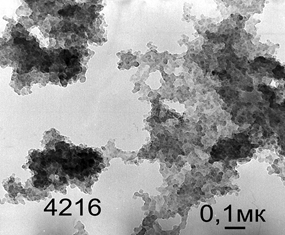
\includegraphics[width=0.8\textwidth]{assets/29}
% 	\caption*{}
% \end{figure}
% 
% \emph{а)}
% \end{minipage} & \begin{minipage}[b]{\linewidth}\raggedright
% \begin{figure}[H]
% 	\centering
% 	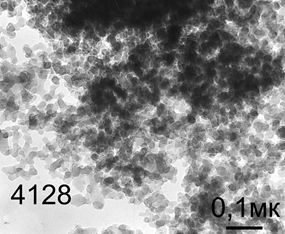
\includegraphics[width=0.8\textwidth]{assets/30}
% 	\caption*{}
% \end{figure}
% 
% \emph{б)}
% \end{minipage} & \begin{minipage}[b]{\linewidth}\raggedright
% \begin{figure}[H]
% 	\centering
% 	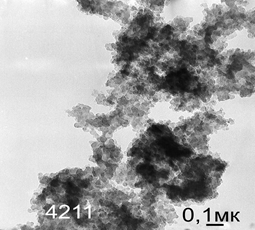
\includegraphics[width=0.8\textwidth]{assets/31}
% 	\caption*{}
% \end{figure}
% 
% \emph{в)}
% \end{minipage} \\
% \midrule\noalign{}
% \endhead
% \bottomrule\noalign{}
% \endlastfoot
% \end{longtable}

{\bfseries 2-сурет. Алынған күйе үлгілері: C/O=1, P=40 Toрр, a) U=0,5 кВ,
б) U=1,0 кВ,}

{\bfseries в) U=2,0 кВ.}

Бұл зерттеулерде қолданылатын электр өрісінің полярлығына қарамастан
электродаралық қашықтықтығы L = 18 см ине-жазықтық электродтарындағы тәж
разряды (газ аралығының жартылай тесілуі) U = 10 кВ дейін сақталды.
Кернеу U = 10 кВ және одан жоғары болған кезде, тәж разряды катод мен
анодты қосатын жарқыраған, ирек жіңішке жіптің пайда болуымен солғын
электр разрядына айналды. Бірақ жалын шебіне солғын электр разрядын
қабат орналастырған кезде, жарқыраған жіп жалынға сіңіп, электродқа
(жандырғыға) жетпей қалды.

Электр өрісінің жалынға әсері теріс полярлық үшін U ≥ 1,35 кВ бастап
(жоғарғы ине-электродта минус) және оң полярлық үшін U ≥ 3,0 кВ (жоғарғы
ине-электродта плюс) визуалды түрде байқалды. Көзге көрінетін әсері
жалынның сығылуымен, тербелісімен, созылуымен, жалпаюымен, қызғалдақ
пішініне айналуымен және басқа да құбылыстардан байқалды. Электр өрісі
болмаған кезде жалын тұрақты, тербеліссіз жанып тұрды, d = 2,5 см, жарық
аймағының биіктігі h = 4,5 см, жандырғыдан бөліну δ = 0,5 см
параметрлері бар цилиндр (жандырғы) пішініне ие болды. Электр өрісін,
мысалы, U = 10 кВ кернеу қолданғанда, жалынның жоғарғы бөлігі толқын
тәрізді тербелетін қызғалдақ тәріздес түрге ие болады.

Осы жұмыста жалынға әсері зерттелген электр өрісі кернеулерінің
диапазонын тиімділігіне қарай шартты түрде екі аймаққа бөлуге болады: I
аймақ - 0,5-тен 3,0 кВ-қа дейін; II аймақ -- 3,0 кВ жоғары.

Бірінші аймақта, күйе шығымы бойынша оң немесе теріс полярлықтың
«тиімділігі» айтарлықтай ерекшеленбейді және күйенің шығу процесі кейде
сәтті, кейде сәтсіз өтті. Бұл жағдайда белгілі бір кернеудегі электр
өрісін қолданғанда күйенің массалық шығымы өріс қолданбағандағы массалық
шығымнан төмен болады. Бұл процесте электр өрісі жану процесіне
каталитикалық әсер береді, сонымен қатар, электр өрісі көмірсутекті
отынның ұзын тізбектерін үзетін күш болып табылады деген гипотезаға
сәйкес келеді.

Алайда, бірінші аймақта электр өрісі кернеулерінің диапазоны
эксперименталды түрде анықталды, оның аймағында күйе түзілудің жоғары
көрсеткіші (шыңы) орын алды және күйенің массалық шығымдылығы (10\%
дейін) электр өрісінің әсерінсіз күйенің шығуынан асып кетті.
Қайталанатын тәжірибелер келтірілген кернеудің полярлығына қарамастан U
= 1,0...1,35 кВ кернеу диапазонында орналасқан жоғарыда келтірілген
тәжірибелік жағдайларда шыңның болуын растады. Бірдей тәжірибелік
жағдайларда күйенің массалық шығымының қайталану қателігі ∆ =1÷ 5 \%
шегінде болды.

Сыртқы электр өрісін берген кезде белсенді орталықтарды пиролиз
аймағынан алып кететін немесе ұстап қалатын күйе түзілу процесі мен
электрлік күштер арасында бәсекелестік әрекеттесу пайда болады және бұл
күйе түзілу кинетикасы үшін ең қолайлы жағдай деп болжауға болады.

Бұл жағдайда берілген кернеудің нәтижесінде күйе бөлшектерінің өсуіне
алып келетін белсенді орталықтар болып табылатын оң
C\textsubscript{n}H\textsubscript{n}\textsuperscript{+} иондарының үлкен
ағыны пиролиз аймағын кесіп өтеді. Берілген кернеудің белгілі бір шектік
мәнінде иондар газ ағынының осьтік компонентасына қатысты қозғалыссыз
деп саналады. Бұл жағдайда күйе бөлшектерінің түзілу жылдамдығы өріс жоқ
жағдаймен салыстырғанда бірнеше есе артады және пиролиз аймағында көзбен
бақыланатын күйе бөлшектері пайда болады. Ұқсас нәтижелер теріс зарядтар
ағынымен де (оң полярлық) алынды.

Берілген кернеулердің екінші аймағында (U \textgreater{} 3 кВ)
полярлыққа қарамастан, U = 3 кВ кернеуіндегі күйе шығымымен
салыстырғанда күйенің массалық шығымының біртіндеп артуы байқалды.
Алайда, жалпы күйе шығымы электр өрісі болмаған жағдайдан төмен болып
қала берді. Бұл кезде күйенің максималды шығымының шыңы байқалмады.
Белсенді орталықтардың түзілуі физикалық және химиялық процестерге
сәйкес келеді, сондықтан бұл аймақта күйе түзілудің мұндай әрекетінің
себебі, мүмкін, қайта зарядталудың термоэлектрондық эмиссияға қарағанда
басым болуынан және белсенді заттардың пиролиз аймағынан шығып кетуінен
туындайды.

{\bfseries Қорытынды.}

1. Зерттеулер көрсеткендей, күрделі құрамды жалынға сыртқы электр
өрісінің әсері жалында болатын процестерді, сондай-ақ, күйе түзілу
процесін бақылауға, сонымен қатар, белгілі бір жағдайларда күйенің
шығымын арттыруға мүмкіндік береді.

2. ИҚ спектроскопиясының көмегімен күйеде фуллерендер
C\textsubscript{60}, C\textsubscript{70} және полициклды ароматтық
көмірсутектер анықталды.

3. С\textsubscript{60} және С\textsubscript{70} фуллерендеріне сәйкес
келетін толқын ұзындықтары оң полярлықпен салыстырғанда теріс полярлықта
айқынырақ анықталғаны көрсетілді. Бұл теріс полярлықтың фуллерендер
шығымына оң полярлыққа қарағанда көбірек әсер ететінін растайды.

4. Спектрлердің интенсивтілігіне сүйене отырып, берілген кернеудің
жоғарылауымен фуллерендердің шығымы жоғарылайтыны анықталды.

{\bfseries Әдебиеттер}

1. Ильюшонок А.В., Гончаренко И.А., Лешенюк Н.С., Кулешов В.К.,
Терешенков В.И.

О влиянии электрического поля на процесс горения. //Вестник Университета
гражданской защиты МЧС Беларуси. 2019. - Т.3( 2) - С.127-137.

2. Степанов Е.М., Дьячков Б.Г. Ионизация в пламени и электрическое поле.
- М.: Металлургия, 1968. - 312 с.

3. Лаутон Дж., Вайнберг Ф. Электрические аспекты горения. Пер. с англ.
Под общ. ред В.А. Попова. - М.: Энергия, 1976. - 296 с.

4. Крестинин А.В., Кислов М.Б., Раевский А.В. и др. K вопросу о
механизме образования сажевых частиц //Кинетика и катализ, 2000. -
Т.41.(1). - С.102-111.

5. Mansurov Z.A., Merkulov A.A., Popov V.T., Tuleutaev B.K., Almazov
N.S. Ultradispersed carbon black formation during methane combustion in
electric field //Khimiya Tverdogo Topliva. 1994. -- Vol. 3. - С. 83-86.

6. Шмелев В.М. О воздействии электрического поля на поверхностное
горение//Химическая физика.- 2016. - Т.35(2).- С. 33-40.

7. Mansurov Z.A., Chenchyk D., Tuleutaev B.K., Mashan T.T. Soot
formation in diffusion flames of acetylene-alkane//International
Symposium on Combustion Abstracts of Works-in-Progress Posters. 2002.
--P.184.

8. Park, D.G., Chung, S.H., Cha, M.S. Visualization of ionic wind in
laminar jet flames. // Combustion and Flame.- 2017.- Vol.184. -
Р.246-248. DOI 10.1016/j.combustflame.2017.06.011.

9. Березкин В.И. Фуллерены как зародыши сажевых частиц. //Физика
твердого тела, 2000. - № 42(3). - С.567-572.

10. Mansurov Z.A. Cool sooting flames of hydrocarbons. //Journal of
Thermal Science.- 2001. - Vol. 10(3). -P.269-280. DOI
10.1007/s11630-001-0031-8

11. Машан Т.Т. Низкотемпературное сажеобразование при горении пропана /
International Scientific and Practical Conference on "Current Problems
of the Chemistry of Coordination Compounds". Bukhara, Uzbekistan.
22-23-december 2022. - P. 488-492.

12. Galeev I.G., Asadullin T.Y. Obtaining fullerene-containing soot
during combustion of gaseous hydrocarbons in an external electric field.
//Journal of Physics Conference Series. VII Conference on low
temperature plasma in the processes of functional coating preparation.
--2016.-Vol.669(1):012016. DOI 10.1088/1742-6596/669/1/012016

{\bfseries References}

1. Il\textquotesingle jushonok A.V., Goncharenko I.A., Leshenjuk N.S.,
Kuleshov V.K., Tereshenkov V.I.

O vlijanii jelektricheskogo polja na process gorenija. //Vestnik
Universiteta grazhdanskoj zashhity MChS Belarusi. 2019. - T.3( 2) -
S.127-137.{[}in Russ.{]}

2.Stepanov E.M., D\textquotesingle jachkov B.G. Ionizacija v plameni i
jelektricheskoe pole. - M.: Metallurgija, 1968. - 312 s. {[}in Russ.{]}

3.Lauton Dzh., Vajnberg F. Jelektricheskie aspekty gorenija. Per. s
angl. Pod obshh. red V.A. Popova. - M.: Jenergija, 1976. - 296 s.{[}in
Russ.{]}

4.Krestinin A.V., Kislov M.B., Raevskij A.V. i dr. K voprosu o mehanizme
obrazovanija sazhevyh chastic //Kinetika i kataliz, 2000. - T.41.(1). -
S.102-111. {[}in Russ.{]}

5. Mansurov Z.A., Merkulov A.A., Popov V.T., Tuleutaev B.K., Almazov
N.S. Ultradispersed carbon black formation during methane combustion in
electric field //Khimiya Tverdogo Topliva. 1994. -- Vol. 3. - С. 83-86.

6. Shmelev V.M. O vozdejstvii jelektricheskogo polja na poverhnostnoe
gorenie//Himicheskaja fizika.- 2016. - T.35(2).- S. 33-40.{[}in Russ.{]}

7. Mansurov Z.A., Chenchyk D., Tuleutaev B.K., Mashan T.T. Soot
formation in diffusion flames of acetylene-alkane//International
Symposium on Combustion Abstracts of Works-in-Progress Posters.- 2002.
-P.184.

8. Park, D.G., Chung, S.H., Cha, M.S. Visualization of ionic wind in
laminar jet flames. // Combustion and Flame.- 2017.-Vol.184. -
Р.246-248. DOI 10.1016/j.combustflame.2017.06.011.

9.Berezkin V.I. Fullereny kak zarodyshi sazhevyh chastic. //Fizika
tverdogo tela, 2000. - №.42(3). - S.567-572

10. Mansurov Z.A. Cool sooting flames of hydrocarbons. //Journal of
Thermal Science.- 2001. - Vol. 10(3). -P.269-280. DOI
10.1007/s11630-001-0031-8

11. Mashan T.T. Nizkotemperaturnoe sazheobrazovanie pri gorenii propana
/ International Scientific and Practical Conference on "Current Problems
of the Chemistry of Coordination Compounds". Bukhara, Uzbekistan.
22-23-december 2022. - P. 488-492.{[}in Russ.{]}

12. Galeev I.G., Asadullin T.Y. Obtaining fullerene-containing soot
during combustion of gaseous hydrocarbons in an external electric field.
//Journal of Physics Conference Series. VII Conference on low
temperature plasma in the processes of functional coating preparation.
--2016.-Vol.669(1):012016. DOI 10.1088/1742-6596/669/1/012016

\emph{{\bfseries Авторлар туралы мәліметтер}}

Машан Т.Т.- химия ғылымдарының кандидаты, химия кафедрасының профессор
м.а., Л.Н. Гумилев атындағы Еуразия ұлттық университеті, Астана,
Қазақстан, e-mail: togzhan-mashan@mail.ru

\emph{{\bfseries Information about the authors}}

Mashan T.T.- Candidate of Chemical Sciences, Acting Professor of the
Department of Chemistry, L.N. Gumilyov Eurasian National University,
Astana, Kazakhstan, e-mail: togzhan-mashan@mail.ru\newpage
{\bfseries IRSTI 31.15.15}

{\bfseries SEMI-EMPIRICAL INVESTIGATION OF ZINC(II) SALICYLATE. COMPARISON
WITH X-RAY STRUCTURE.}

{\bfseries N. Akatyev}

M.Utemisov West Kazakhstan university, Uralsk, Kazakhstan,

Corresponding author: nikolay.akatyev@wku.edu.kz

Zinc salicylate dihydrate
(Zn(HSal)\textsubscript{2}·2H\textsubscript{2}O) is an organic-inorganic
hybrid compound known for its wide range of applications. In this
article, a detailed semiempirical study of zinc salicylate is presented,
focusing on its structural, electronic, and thermodynamic properties.
The PM3 method, known for its computational efficiency and reasonable
accuracy, was used to model the molecular structure and compare with the
experimentally obtained properties of
Zn(HSal)\textsubscript{2}·2H\textsubscript{2}O. Based on the obtained
calculation results and available experimental data published in the
literature, it was found that semi-empirical calculations involving the
solvent effect (H\textsubscript{2}O) agree well with data from X-ray
diffraction analysis, while calculations for the gas phase do not agree
with experimental data with the required accuracy. Quantum chemical
descriptors such as HOMO-LUMO energies, energy gap
(ΔE\textsubscript{gap}), electronegativity (χ), global hardness (η),
softness (σ), dipole moment (μ), electrophilic (ω) and nucleophilic (ε)
indices were also calculated. The results show that the PM3 method
effectively captures the essential features of zinc salicylate,
including its geometry and electronic distribution. The obtained results
also provide valuable insights into the semi-empirical modeling of
organometallic compounds and highlight the usefulness of the PM3 method
in predicting the behavior of complex molecular systems.

{\bfseries Keywords:} PM3 calculations, zinc salicylate, semi-empirical
calculations, quantum chemical descriptors.

{\bfseries МЫРЫШ(II) САЛИЦИЛАТЫН ЖАРТЫЛАЙ ЭМПИРИКАЛЫҚ ЗЕРТТЕУ. РЕНТГЕН
ҚҰРЫЛЫМЫМЕН САЛЫСТЫРУ.}

{\bfseries Н. Акатьев}

М.Өтемісов атындағы Батыс Қазақстан университеті, Орал, Қазақстан,

e-mail: nikolay.akatyev@wku.edu.kz

Мырыш салицилат дигидраты
(Zn(HSal)\textsubscript{2}·2H\textsubscript{2}O), қолдану аясының кең
ауқымымен танымал органикалық-бейорганикалық гибридті қосылыс. Бұл
мақалада оның құрылымдық, электронды және термодинамикалық қасиеттеріне
назар аудара отырып, мырыш салицилатының егжей-тегжейлі жартылай
эмпирикалық зерттеуі ұсынылған. Молекулярлық құрылымды модельдеу және
Zn(HSal)\textsubscript{2}·2H\textsubscript{2}O-ның тәжірибелік алынған
қасиеттерімен салыстыру үшін өзінің есептеу тиімділігі мен ақылға
қонымды дәлдігімен танымал PM3 әдісі қолданылды. Алынған есептеу
нәтижелеріне және әдебиетте жарияланған қолда бар эксперименттік
деректерге сүйене отырып, еріткіш әсерін (H\textsubscript{2}O) қамтитын
жартылай эмпирикалық есептеулер рентгендік дифракциялық талдау
деректерімен жақсы сәйкес келеді, ал газ фазасы үшін есептеулер сәйкес
келмейтіні анықталды. қажетті дәлдікпен эксперименттік деректермен.
HOMO-LUMO энергиясы, энергетикалық алшақтық (ΔE\textsubscript{gap}),
электртерістілік (χ), ғаламдық қаттылық (η), жұмсақтық (σ), дипольдік
момент (μ), электрофильдік (ω) және нуклеофильдік (ε) индекстері сияқты
кванттық химиялық дескрипторлар да болды. есептелген. Нәтижелер PM3
әдісі мырыш салицилатының маңызды ерекшеліктерін, соның ішінде оның
геометриясын және электрондық таралуын тиімді түрде түсіретінін
көрсетеді. Алынған нәтижелер сонымен қатар металлорганикалық
қосылыстардың жартылай эмпирикалық модельделуіне құнды түсініктер береді
және күрделі молекулалық жүйелердің әрекетін болжауда РМ3 әдісінің
пайдалылығын көрсетеді.

{\bfseries Түйін сөздер:} РМ3 есептеулері, мырыш салицилаты, жартылай
эмпирикалық есептеулер, кванттық химиялық дескрипторлар.

{\bfseries ПОЛУЭМПИРИЧЕСКОЕ ИССЛЕДОВАНИЕ САЛИЦИЛАТА ЦИНКА(II). СРАВНЕНИЕ С
РЕНТГЕНОВСКОЙ СТРУКТУРОЙ.}

{\bfseries Н. Акатьев}

Западно-Казахстанский университет им.М.Утемисова, Уральск, Казахстан,

e-mail: nikolay.akatyev@wku.edu.kz

Дигидрат салицилата цинка
(Zn(HSal)\textsubscript{2}·2H\textsubscript{2}O)- гибридное
органо-неорганическое соединение, известное своим широким спектром
применения. В данной статье представлено подробное полуэмпирическое
исследование салицилата цинка с упором на его структурные, электронные и
термодинамические свойства. Для моделирования молекулярной структуры и
сравнения с экспериментально полученными свойствами
Zn(HSal)\textsubscript{2}·2H\textsubscript{2}O был использован метод
PM3, известный своей вычислительной эффективностью и приемлемой
точностью. На основании полученных расчётов и имеющихся
экспериментальных данных, опубликованных в литературе, установлено, что
полуэмпирические расчёты с учетом эффекта растворителя
(H\textsubscript{2}O) хорошо согласуются с данными рентгеноструктурного
анализа, тогда как расчеты для газовой фазы не согласуются с
экспериментальными данными с необходимой точностью. Были рассчитаны
квантово-химические дескрипторы, такие как энергии ВЗМО-НВМО,
энергетическая щель (ΔE\textsubscript{gap}), электроотрицательность (χ),
глобальная твердость (η), мягкость (σ), дипольный момент (μ),
электрофильные (ω) и нуклеофильные (ε) индексы. Результаты показывают,
что метод PM3 эффективно отражает основные характеристики салицилата
цинка, включая его геометрию и электронное распределение. Полученные
результаты также дают ценную информацию о полуэмпирическом моделировании
металлоорганических соединений и подчеркивают полезность метода PM3 для
прогнозирования поведения сложных молекулярных систем.

{\bfseries Ключевые слова:} PM3 расчёты, салицилат цинка, полуэмпирические
расчёты, квантово-химические дескрипторы.

{\bfseries Introduction.} Numerous branches of chemistry place significant
theoretical and practical emphasis on the structure and characteristics
of transition metal salicylates. These simple organic salts of salicylic
acid (\emph{o}-hydroxybenzoic acid) have a wide range of applications
because of their beneficial qualities. Compounds with carboxyl groups
are intriguing from the standpoint of coordination chemistry because
they can bind to metal ions as mono-, bi-, and bridging ligands.

Over the last two decades, a wide range of transition metal complexes
containing salicylate and its various derivatives have been described.
Das \emph{et al.} reported a highly porous and thermally stable Co(II)
salicylate metal--organic framework (MOF). Obtained material has very
interesting magnetic properties, in which the magnetic moments increase
with decreasing temperature {[}1{]}. A metal-containing ionic liquid
(MCIL) has been also prepared in which the
{[}Co\textsuperscript{II}(Sal)\textsubscript{2}{]}\textsuperscript{2-}
anion is able to selectively coordinate two water molecules with a
visible color change {[}2{]}. Chakraborty and Paine synthesized and
structurally characterized four mononuclear cobalt-salicylate complexes
derived from N4-donor ligands. A hexameric water cluster is stabilized
in the lattice of hydrated crystal complex {[}3{]}. A manganese complex
with a salicylic acid residue was reported by Devereux \emph{et al}. In
the presence of imidazole, the complex powerfully catalyzes the
disproportionation of hydrogen peroxide {[}4{]}. Square-planar
bis(N,N-dimethylbiguanide)nickel(II) salicylate and
hexakis(imidazole)nickel(II) disalicylate were also reported by Lemoine
{[}5{]} and Jian {[}6{]} respectively. Copper salicylate is known as an
anti-inflammatory agent {[}7{]}.

Zinc is an essential trace element in the human body for activating (as
a cofactor) more than 200 zinc-dependent metalloenzymes {[}8{]}. In
addition, zinc is urgently needed for human health due to its critical
role in growth, metabolism and wound healing {[}9,10{]}. It is the
second most abundant micronutrient in the human body after iron
{[}11{]}. Zinc also plays a central role in plant defense against
pathogens and herbivores {[}12{]}. Nevertheless, overaccumulation of
zinc leads to morphological, biochemical, and physiological disorders
and can be toxic to flora, fauna and humans {[}13{]}.

Zinc salicylate is interesting for its biological activity. It is known
as a component of antifouling coatings and has been demonstrated by
Bellotti and Romagnoli to be effective against \emph{Artemia larvae}
with lower toxicity than copper {[}14{]}. Fang compared the zinc
salicylate-methylsulfonylmethane complex with zinc salicylate, sodium
salicylate and zinc chloride in terms of the remodeling parameters of
human airway smooth muscle cells (ASMC) {[}15{]}. In addition, zinc
salicylate is described as a carbon source for templating porous carbons
for supercapacitors {[}16{]}. Some other zinc salicylate-derived
complexes have been studied by Brownless {[}17{]} and Chooset {[}18{]}.

In contemporary theoretical science, the quantum chemical approach is
used to extend on experimental investigations and to find appropriate
theoretical parameters to describe or interpret the experimental
results. On the other hand, computational methods make it possible to
predict the variety of practically important properties of substances
and complex systems based on electronic density, charge distribution or
other descriptors. Techniques based on density functional theory (DFT)
have long been used to study the electronic structure of transition
metal compounds. However, this approach is still extremely
computationally intensive and may not be practical for many systems of
interest {[}19{]}. Semi-empirical methods are much faster and therefore
have great potential to produce acceptable results. Higher speed comes
at the expense of the approximations made in evaluating the integrals
describing the interactions between nuclei and some electron integrals
of the electrons (considered negligible) are ignored while others are
estimated from experiments {[}20{]}. In our research, we used the
semi-empirical quantum chemical method PM3 to investigate the properties
of the zinc (II) salicylate dihydrate Zn(HSal)\textsubscript{2} ·
2H\textsubscript{2}O.

{\bfseries Materials and methods.} Like other semi-empirical methods, PM3
is a self-consistent-field (SCF) method. All calculated integrals are
evaluated using approximate values. Semiempirical calculations of
transition metal complexes are orders of magnitude cheaper than their
\emph{ab initio} and most DFT counterparts and are extremely productive
in the field of theoretical organic chemistry. However, the
parameterization of these methods for transition metal systems is not
trivial. Nevertheless, some attempts have been made to introduce
\emph{d}-orbitals into traditional semi-empirical methods. The PM3
method has a range of parameters for transition metals {[}21{]}. It is
the most applicable semi-empirical method for calculating zinc compounds
with Zn\textsuperscript{+2}. AM1 produces errors 30\% larger than PM3.
Owing to errors in its original parametrization, MNDO/d is not
appropriate for use in computations {[}22{]}.

All quantum chemical calculations were performed on a desktop PC with
Windows 11, a 12\textsuperscript{th} generation Intel(R) Core (TM)
i7-12700H 2.30 GHz, 16GB RAM) with GAMESS software {[}23{]}. The
programs Avogadro {[}24{]} and Jmol {[}25{]} were used to prepare the
input file and visualize the results respectively. Initially, full
geometry optimization was achieved using the Molecular Mechanics (MM+)
force field in the gas phase. The results from MM+ were further selected
as input and re-optimized using semi-empirical PM3 {[}26{]} to obtain
the equilibrium geometry with a root mean square (RMS) gradient of 0.001
kcal/Å·mol. This calculation method requires little computational effort
and provides good agreement with the experiment. Semiempirical methods
can be applied to calculations of much larger systems than classical
\emph{ab initio} or DFT methods, sometimes achieving accuracy comparable
to more advanced levels of theory {[}27{]}. Method based on neglecting
the integral approximation of differential diatomic overlap,
representing an excellent compromise between completeness and economy.
The molecular geometry was fully optimized using the analytical gradient
method implemented in the program package without any limitations. The
computational study was carried out in the gas and solution phases.
Water was used to incorporate the solvent effect. To better approximate
the experimental results in the solution phase, Tomasi\textquotesingle s
Polarized Continuum Model PCM was used.

The following quantum chemical indices, describing global reactivity
were considered: the energy of the highest occupied molecular orbital
(E\emph{\textsubscript{HOMO}}), the energy of the lowest unoccupied
molecular orbital (E\emph{\textsubscript{LUMO}}), energy gap
(ΔE\textsubscript{gap}), the ionization potential (IP), the electron
affinity (EA), electronegativity (χ), global hardness (η), softness (σ),
dipole moment (μ), electrophilic (ω) and nucleophilic (ε) indexes. They
were calculated using formulas 1-8:

ΔE\textsubscript{gap} = E\emph{\textsubscript{LUMO}} -
E\emph{\textsubscript{HOMO}} (1)

IP = - E\emph{\textsubscript{HOMO}} (2)

EA = - E\emph{\textsubscript{LUMO}} (3)

\begin{figure}[H]
	\centering
	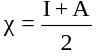
\includegraphics[width=0.8\textwidth]{assets/32}
	\caption*{}
\end{figure} (4)

\begin{figure}[H]
	\centering
	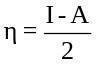
\includegraphics[width=0.8\textwidth]{assets/33}
	\caption*{}
\end{figure} (5)

\begin{figure}[H]
	\centering
	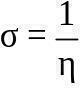
\includegraphics[width=0.8\textwidth]{assets/34}
	\caption*{}
\end{figure} (6)

\begin{figure}[H]
	\centering
	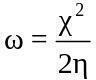
\includegraphics[width=0.8\textwidth]{assets/35}
	\caption*{}
\end{figure} (7)

\begin{figure}[H]
	\centering
	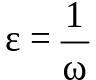
\includegraphics[width=0.8\textwidth]{assets/36}
	\caption*{}
\end{figure} (8)

According to the Koopman's theorem, the HOMO energy is related to IP
while the LUMO energy is related to EA (Eq. 2, 3). Electronegativity (χ)
and global hardness (η) were evaluated based on the finite difference
approximation as linear combinations of the calculated IP and EA
{[}28{]} (Eq. 4, 5). The global softness (σ) is the reciprocal of the
global hardness {[}29{]} (Eq. 6). The global electrophilicity index (ω)
describes the stabilization of a molecule after the acquisition of an
additional number of electrons (Eq. 7). The nucleophilicity index (ε) is
the reciprocal of the global electrophilicity index (Eq. 8).

{\bfseries Results and discussion.} The aim of this research is to study
Zn(HSal)\textsubscript{2}·2H\textsubscript{2}O in the gas and aqueous
phases from a structural and energetic perspective using quantum
chemical descriptors calculated using the semi-empirical PM3 method.
Another aim is to compare the calculated geometry with the available
detailed X-ray structural data obtained by Gusev \emph{et al} {[}30{]}.
The molecular structure is close to
Zn(HSal)\textsubscript{2}·2H\textsubscript{2}O (Figure 1). The substance
belongs to the space group C\textsubscript{2} and the monoclinic crystal
system.

\begin{figure}[H]
	\centering
	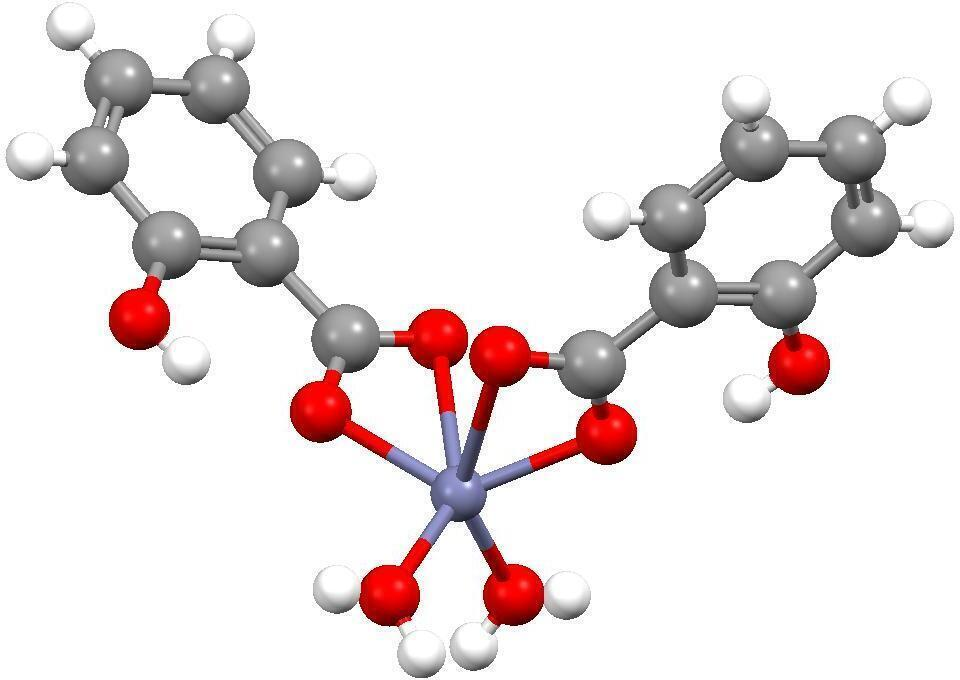
\includegraphics[width=0.8\textwidth]{assets/37}
	\caption*{}
\end{figure}\begin{figure}[H]
	\centering
	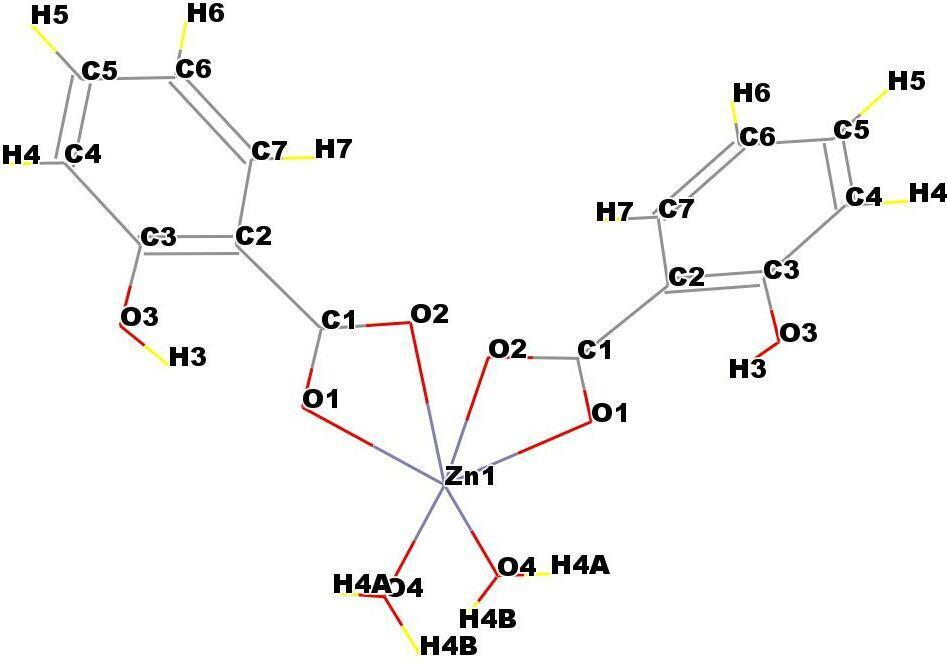
\includegraphics[width=0.8\textwidth]{assets/38}
	\caption*{}
\end{figure}

{\bfseries Figure 1 - Structural formula of the
Zn(HSal)\textsubscript{2}·2H\textsubscript{2}O molecule obtained with
X-ray diffraction by Gusev \emph{et al}.}

The crystal structure of zinc (II) salicylate dihydrate was first
described by Klug {[}31{]}. The thermal behavior of zinc salicylate and
5-chlorosalicylate complexes with bioactive ligands was studied by
Chomič \emph{et al} {[}32,33{]}\emph{.} The stability constant of zinc
(II) salicylate was determined by Singh {[}34{]}.

{\bfseries \emph{Bond length.}} As part of our investigation, we first
presented the PM3-optimized geometry parameters (bond length and angle)
in the gas and aqueous phases in comparison to available X-ray analysis
data. The calculated and experimental values \hspace{0pt}\hspace{0pt}of
the bond lengths are listed in Table 1. The list of atoms corresponds to
Figure 1.

{\bfseries Table 1 - Comparison between experimental X-ray and PM3
calculated bond lengths (Å) of
Zn(HSal)\textsubscript{2}·2H\textsubscript{2}O for the gas and aqueous
phases.}

\begin{longtable}[]{@{}
  >{\raggedright\arraybackslash}p{(\columnwidth - 8\tabcolsep) * \real{0.1602}}
  >{\raggedright\arraybackslash}p{(\columnwidth - 8\tabcolsep) * \real{0.1602}}
  >{\raggedright\arraybackslash}p{(\columnwidth - 8\tabcolsep) * \real{0.2012}}
  >{\raggedright\arraybackslash}p{(\columnwidth - 8\tabcolsep) * \real{0.2031}}
  >{\raggedright\arraybackslash}p{(\columnwidth - 8\tabcolsep) * \real{0.2752}}@{}}
\toprule\noalign{}
\multirow{2}{=}{\begin{minipage}[b]{\linewidth}\raggedright
{\bfseries Atom 1}
\end{minipage}} &
\multirow{2}{=}{\begin{minipage}[b]{\linewidth}\raggedright
{\bfseries Atom 2}
\end{minipage}} &
\multicolumn{3}{>{\raggedright\arraybackslash}p{(\columnwidth - 8\tabcolsep) * \real{0.6795} + 4\tabcolsep}@{}}{%
\begin{minipage}[b]{\linewidth}\raggedright
{\bfseries Bond length, Å}
\end{minipage}} \\
& & \begin{minipage}[b]{\linewidth}\raggedright
{\bfseries XRD data}
\end{minipage} & \begin{minipage}[b]{\linewidth}\raggedright
{\bfseries Gas phase}
\end{minipage} & \begin{minipage}[b]{\linewidth}\raggedright
{\bfseries Aqueous phase}
\end{minipage} \\
\midrule\noalign{}
\endhead
\bottomrule\noalign{}
\endlastfoot
Zn1 & O1 & 1.9928 & 2.1156 & 1.9897 \\
Zn1 & O2 & 2.5679 & 2.3277 & 2.5815 \\
Zn1 & O4 & 1.9857 & 2.3194 & 2.0294 \\
Zn1 & O1 & 1.9928 & 2.1156 & 1.9897 \\
Zn1 & O2 & 2.5679 & 2.2659 & 2.5815 \\
Zn1 & O4 & 1.9857 & 2.3042 & 2.0294 \\
O1 & C1 & 1.2830 & 1.3328 & 1.2651 \\
O2 & C1 & 1.2533 & 1.2584 & 1.2312 \\
O3 & C3 & 1.3641 & 1.3760 & 1.3874 \\
O3 & H3 & 0.7692 & 0.9580 & 0.7716 \\
O4 & H4A & 0.6499 & 0.9452 & 0.6498 \\
O4 & H4B & 0.8521 & 0.9413 & 0.8136 \\
C1 & C2 & 1.4796 & 1.4894 & 1.4682 \\
C7 & H7 & 0.9306 & 1.1000 & 0.9077 \\
C7 & C2 & 1.4039 & 1.3953 & 1.4079 \\
C7 & C6 & 1.3806 & 1.3940 & 1.4053 \\
C3 & C2 & 1.4065 & 1.3394 & 1.3907 \\
C3 & C4 & 1.3874 & 1.4232 & 1.3667 \\
C5 & H5 & 0.9303 & 1.1108 & 0.9208 \\
C5 & C6 & 1.3964 & 1.3451 & 1.3966 \\
C5 & C4 & 1.3860 & 1.3396 & 1.3737 \\
C6 & H6 & 0.9305 & 1.0886 & 0.8965 \\
C4 & H4 & 0.9291 & 1.1186 & 0.8952 \\
O1 & C1 & 1.2830 & 1.3328 & 1.2651 \\
O2 & C1 & 1.2532 & 1.2584 & 1.2312 \\
O3 & C3 & 1.3641 & 1.3760 & 1.3874 \\
O3 & H3 & 0.7691 & 0.9580 & 0.7716 \\
O4 & H4A & 0.6499 & 0.9452 & 0.6498 \\
O4 & H4B & 0.8521 & 0.9413 & 0.8136 \\
C1 & C2 & 1.4796 & 1.4894 & 1.4682 \\
C7 & H7 & 0.9306 & 1.1000 & 0.9077 \\
C7 & C2 & 1.4039 & 1.3953 & 1.4079 \\
C7 & C6 & 1.3806 & 1.3940 & 1.4053 \\
C3 & C2 & 1.4065 & 1.3394 & 1.3907 \\
C3 & C4 & 1.3874 & 1.4232 & 1.3667 \\
C5 & H5 & 0.9303 & 1.1108 & 0.9208 \\
C5 & C6 & 1.3964 & 1.3451 & 1.3966 \\
C5 & C4 & 1.3861 & 1.3396 & 1.3737 \\
C6 & H6 & 0.9305 & 1.0886 & 0.8965 \\
C4 & H4 & 0.9292 & 1.1186 & 0.8952 \\
\end{longtable}

A comparison of the calculated bond lengths of zinc salicylate with
X-ray structural data shows that they agree well in the case of the
aqueous phase. For example, the calculated length of the Zn1-O1 bond is
1.9897Å while the experimental value is 1.9928Å. These values lie within
acceptable deviations. Bond length values
\hspace{0pt}\hspace{0pt}calculated for the gas phase are less consistent
with experimental results. In addition, the calculated bond lengths of
the zinc salicylate molecule in the gas phase are slightly longer than
in aqueous phase. An exception are the Zn(1)-O(4) coordination bonds and
the O-H-bond in coordinated water molecules, whose lengths were
significantly longer for the gas phase.

The lengths of the C=C bonds in the benzene ring are typical for
aromatic compounds. The calculated length also agrees well with the
reference data.

{\bfseries \emph{Bond angles.}} Experimental and calculated values of the
bond angles are listed in Table 2.

{\bfseries Table 2 - Bond angle properties of
Zn(HSal)\textsubscript{2}·2H\textsubscript{2}O obtained from XRD and
calculated using the PM3 method.}

\begin{longtable}[]{@{}
  >{\raggedright\arraybackslash}p{(\columnwidth - 10\tabcolsep) * \real{0.1454}}
  >{\raggedright\arraybackslash}p{(\columnwidth - 10\tabcolsep) * \real{0.1454}}
  >{\raggedright\arraybackslash}p{(\columnwidth - 10\tabcolsep) * \real{0.1454}}
  >{\raggedright\arraybackslash}p{(\columnwidth - 10\tabcolsep) * \real{0.1658}}
  >{\raggedright\arraybackslash}p{(\columnwidth - 10\tabcolsep) * \real{0.1675}}
  >{\raggedright\arraybackslash}p{(\columnwidth - 10\tabcolsep) * \real{0.2304}}@{}}
\toprule\noalign{}
\multirow{2}{=}{\begin{minipage}[b]{\linewidth}\raggedright
{\bfseries Atom 1*}
\end{minipage}} &
\multirow{2}{=}{\begin{minipage}[b]{\linewidth}\raggedright
{\bfseries Atom 2*}
\end{minipage}} &
\multirow{2}{=}{\begin{minipage}[b]{\linewidth}\raggedright
{\bfseries Atom 3*}
\end{minipage}} &
\multicolumn{3}{>{\raggedright\arraybackslash}p{(\columnwidth - 10\tabcolsep) * \real{0.5637} + 4\tabcolsep}@{}}{%
\begin{minipage}[b]{\linewidth}\raggedright
{\bfseries Bond angle (deg)}
\end{minipage}} \\
& & & \begin{minipage}[b]{\linewidth}\raggedright
{\bfseries XRD data}
\end{minipage} & \begin{minipage}[b]{\linewidth}\raggedright
{\bfseries Gas phase}
\end{minipage} & \begin{minipage}[b]{\linewidth}\raggedright
{\bfseries Aqueous phase}
\end{minipage} \\
\midrule\noalign{}
\endhead
\bottomrule\noalign{}
\endlastfoot
O1 & Zn1 & O2 & 56.03 & 57.27 & 55.07 \\
O1 & Zn1 & O4 & 120.11 & 112.40 & 119.68 \\
O1 & Zn1 & O1 & 128.18 & 145.40 & 127.48 \\
O1 & Zn1 & O2 & 86.98 & 99.58 & 85.12 \\
O1 & Zn1 & O4 & 92.86 & 91.74 & 90.46 \\
O2 & Zn1 & O4 & 91.72 & 90.81 & 90.85 \\
O2 & Zn1 & O1 & 86.98 & 99.90 & 85.12 \\
O2 & Zn1 & O2 & 91.21 & 99.56 & 90.54 \\
O2 & Zn1 & O4 & 148.53 & 147.68 & 147.65 \\
O4 & Zn1 & O1 & 92.86 & 88.28 & 90.46 \\
O4 & Zn1 & O2 & 148.53 & 143.73 & 147.65 \\
O4 & Zn1 & O4 & 101.74 & 91.92 & 101.00 \\
O1 & Zn1 & O2 & 56.03 & 57.27 & 55.07 \\
O1 & Zn1 & O4 & 120.11 & 114.71 & 119.68 \\
O2 & Zn1 & O4 & 91.72 & 94.38 & 90.85 \\
Zn1 & O1 & C1 & 104.47 & 98.21 & 104.94 \\
Zn1 & O2 & C1 & 78.62 & 91.07 & 77.49 \\
C3 & O3 & H3 & 106.76 & 107.91 & 104.75 \\
Zn1 & O4 & H4A & 114.69 & 100.15 & 111.15 \\
Zn1 & O4 & H4B & 120.35 & 102.46 & 120.99 \\
H4A & O4 & H4B & 122.19 & 101.98 & 121.35 \\
O1 & C1 & O2 & 120.46 & 111.12 & 121.99 \\
O1 & C1 & C2 & 118.01 & 121.43 & 117.24 \\
O2 & C1 & C2 & 121.51 & 121.71 & 120.72 \\
H7 & C7 & C2 & 119.30 & 119.59 & 118.93 \\
H7 & C7 & C6 & 119.30 & 120.93 & 119.60 \\
C2 & C7 & C6 & 121.40 & 120.25 & 119.55 \\
O3 & C3 & C2 & 121.63 & 123.88 & 121.59 \\
O3 & C3 & C4 & 117.81 & 128.18 & 117.40 \\
C2 & C3 & C4 & 120.56 & 120.39 & 120.88 \\
C1 & C2 & C7 & 120.06 & 120.34 & 120.28 \\
C1 & C2 & C3 & 121.64 & 120.60 & 121.20 \\
C7 & C2 & C3 & 118.23 & 119.44 & 118.47 \\
H5 & C5 & C6 & 119.70 & 119.83 & 117.08 \\
H5 & C5 & C4 & 119.72 & 119.37 & 119.23 \\
C6 & C5 & C4 & 120.58 & 116.83 & 121.68 \\
C7 & C6 & C5 & 119.26 & 120.35 & 118.71 \\
C7 & C6 & H6 & 120.34 & 119.77 & 119.83 \\
C5 & C6 & H6 & 120.40 & 116.49 & 120.69 \\
C3 & C4 & C5 & 119.96 & 129.69 & 118.94 \\
C3 & C4 & H4 & 120.00 & 119.77 & 120.06 \\
C5 & C4 & H4 & 120.04 & 114.33 & 120.96 \\
Zn1 & O1 & C1 & 104.47 & 96.94 & 104.96 \\
Zn1 & O2 & C1 & 78.62 & 98.38 & 77.49 \\
C3 & O3 & H3 & 106.77 & 106.71 & 104.75 \\
Zn1 & O4 & H4A & 114.69 & 102.46 & 111.15 \\
Zn1 & O4 & H4B & 120.34 & 100.65 & 120.99 \\
H4A & O4 & H4B & 122.20 & 108.95 & 121.35 \\
O1 & C1 & O2 & 120.46 & 111.12 & 121.99 \\
O1 & C1 & C2 & 118.01 & 121.30 & 117.24 \\
O2 & C1 & C2 & 121.51 & 121.71 & 120.72 \\
H7 & C7 & C2 & 119.30 & 119.41 & 118.93 \\
H7 & C7 & C6 & 119.30 & 122.79 & 119.60 \\
C2 & C7 & C6 & 121.40 & 120.46 & 119.55 \\
O3 & C3 & C2 & 121.63 & 124.63 & 121.59 \\
O3 & C3 & C4 & 117.81 & 128.18 & 117.40 \\
C2 & C3 & C4 & 120.56 & 120.21 & 120.88 \\
C1 & C2 & C7 & 120.06 & 120.55 & 120.28 \\
C1 & C2 & C3 & 121.64 & 120.29 & 121.20 \\
C7 & C2 & C3 & 118.23 & 119.44 & 118.47 \\
H5 & C5 & C6 & 119.70 & 119.56 & 117.08 \\
H5 & C5 & C4 & 119.72 & 123.61 & 119.23 \\
C6 & C5 & C4 & 120.57 & 116.83 & 121.68 \\
C7 & C6 & C5 & 119.26 & 120.37 & 118.71 \\
C7 & C6 & H6 & 120.34 & 119.72 & 119.83 \\
C5 & C6 & H6 & 120.39 & 121.05 & 120.69 \\
C3 & C4 & C5 & 119.96 & 119.70 & 118.94 \\
C3 & C4 & H4 & 120.00 & 119.43 & 120.06 \\
C5 & C4 & H4 & 120.04 & 121.11 & 120.96 \\
\end{longtable}

* - \emph{numbering of atoms is in accordance with Fig.1.}

A comparison of the results of the PM3 zinc salicylate bond angle
calculations show the same trend as the results of the bond length
calculations. The angle values \hspace{0pt}\hspace{0pt}obtained for the
aqueous phase agree well with the X-ray diffraction results. The
calculation for the gas phase shows a significantly lower correlation to
experimental data. It can be clearly concluded that the best results for
calculating the geometry of such molecules can be obtained for the
solution phase. In this case, gas phase calculations are performed with
significant errors.

\emph{{\bfseries Mulliken charges population analysis.}} The local
reactivity of zinc salicylate was studied using Mulliken charge
population analysis, which provides an indication of the reactive
(nucleophilic and electrophilic) centers of molecules. Therefore, the
regions of the molecule with high electronic charge are chemically
softer than the regions with low electronic charge, so electron density
plays an important role in chemical reactivity calculations. The results
of the Mulliken atomic charge calculation are shown in Figure 2.

% TODO
%\begin{figure}[H]
%	\centering
%	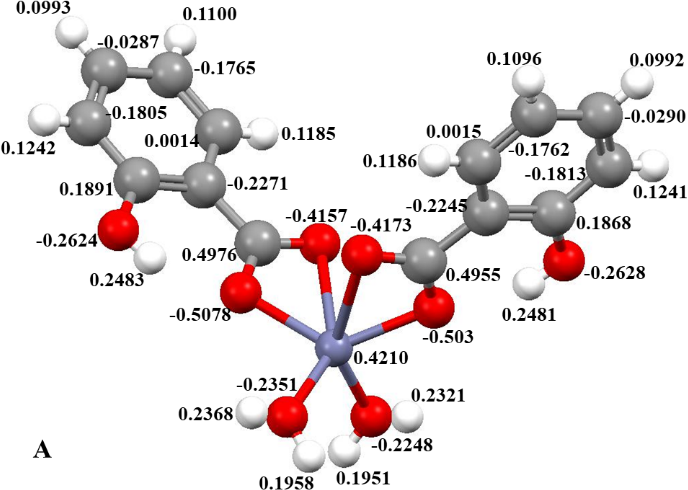
\includegraphics[width=0.8\textwidth]{assets/39}
%	\caption*{}
%\end{figure}\begin{figure}[H]
%	\centering
%	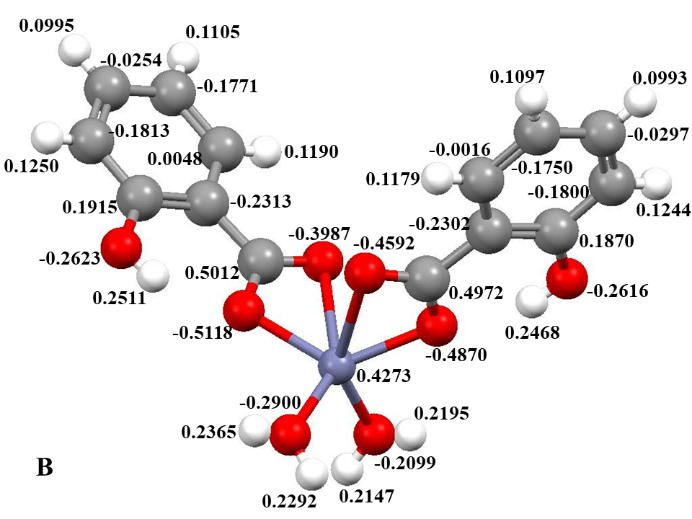
\includegraphics[width=0.8\textwidth]{assets/40}
%	\caption*{}
%\end{figure}

{\bfseries Figure 2 - PM3 Mulliken charges population for the calculated
Zn(HSal)\textsubscript{2}·2H\textsubscript{2}O molecule in gas (A) and
aqueous (B) phase.}

The place for a nucleophilic attack is where the value of the positive
charge is maximum. The location of electrophilic attack is in turn
controlled by the negative charge value. Mulliken charge population
analysis shows that the zinc atoms in both the gas and aqueous phases
have the maximum positive charge. The most negative charges are on the
oxygen atoms of the carboxyl groups. Consequently, the oxygen atoms of
the carboxyl groups are most susceptible to electrophilic attack. The
presence of water leads to a slight shift in the electron density
towards the oxygen atoms of the carboxyl groups, which becomes more
negative.

\emph{{\bfseries Frontier molecular orbitals (FMO).}} Frontier orbital
theory is very useful for determining the main properties of molecules.
The positions of the highest occupied molecular orbital (HOMO) and the
lowest unoccupied molecular orbital (LUMO) are molecular parameters that
are directly related to the electron and hole transport properties of
the substance. The energy gap value (ΔE\textsubscript{gap}) is the
difference between HOMO-LUMO and is used as a significant descriptor of
molecular stability. The most stable molecule has a low
ΔE\textsubscript{gap}.

The molecular electrostatic potential (MEP), frontier molecular orbitals
energies and ΔE\textsubscript{gap} calculated for
Zn(HSal)\textsubscript{2}·2H\textsubscript{2}O are shown in Figure 3.

\begin{figure}[H]
	\centering
	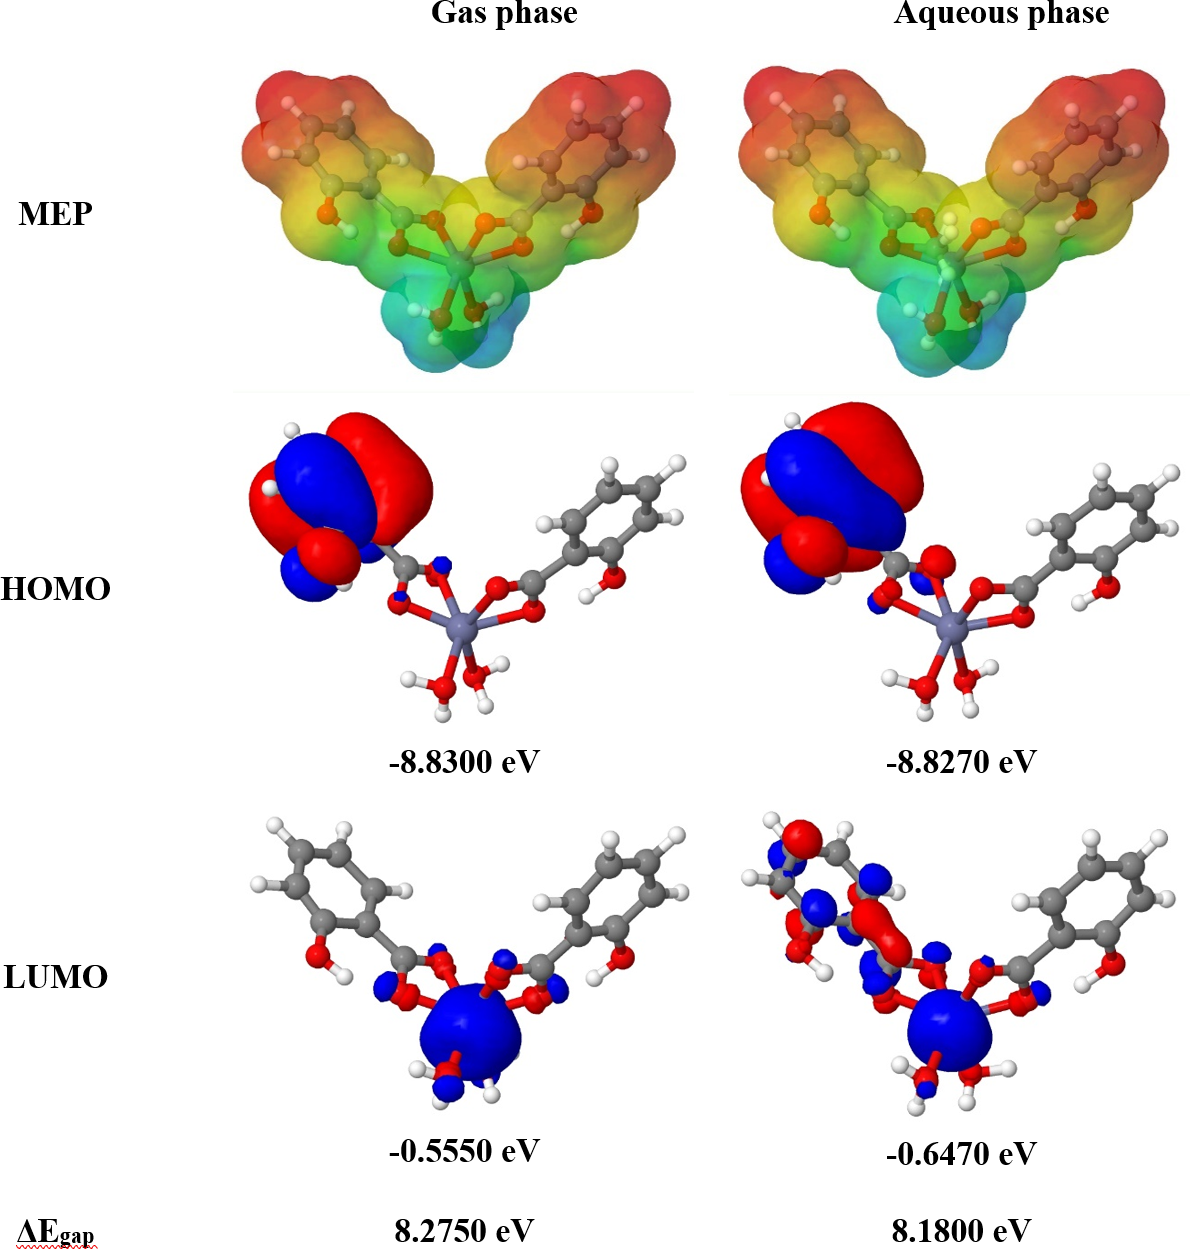
\includegraphics[width=0.8\textwidth]{assets/41}
	\caption*{}
\end{figure}

{\bfseries Figure 3 - The molecular electrostatic potential (MEP) and
frontier molecular orbitals (HOMO-LUMO) density distribution of the
Zn(HSal)\textsubscript{2}·2H\textsubscript{2}O calculated with PM3 for
gas and aqueous phases.}

The positively charged lobe is indicated by the blue color, and the
negatively charged lobe is indicated by the red color.

E\textsubscript{HOMO} describes the electron donating ability of the
molecule. Conversely, E\textsubscript{LUMO} describes the ability of the
molecule to accept electrons. The lower the LUMO value, the higher the
ability of the compound to accept electrons. The HOMOs of
Zn(HSal)\textsubscript{2}·2H\textsubscript{2}O are mainly located at the
oxygen atoms of the -OH-group in the ortho-position. On the other hand,
the LUMOs are mainly located on the zinc atoms and oxygen atoms of the
carboxyl units. The presence of water as a high dielectric constant
model solvent results in a slight decrease in the LUMO energy (around
0.095 eV) and a non-significant decrease in the HOMO energy.

Negative values for E\textsubscript{HOMO} and E\textsubscript{LUMO}
indicate the presence of additional electron pairs in both the upper and
lower molecular orbitals. This means that zinc salicylate should act as
an electron donor in chemical transformations. A low negative LUMO value
(near zero) indicates that zinc salicylate is a weak electrophile.

The gap energy (ΔE\textsubscript{gap}, Eq.1.) between the frontier
orbitals is usually of great importance in describing static molecular
reactivity. Large energy gap values \hspace{0pt}\hspace{0pt}mean high
electronic stability and therefore low reactivity. In the gas phase,
zinc salicylate has a higher ΔE\textsubscript{gap} value than in
solution (8.275 eV and 8.180 eV respectively). Therefore, zinc
salicylate is more stable in the gas phase than in solution. Under the
influence of polar water molecules, zinc salicylate becomes unstable as
it dissolves and dissociates into ions.

{\bfseries \emph{Quantum chemical descriptors.}} In accordance with the
relationship of HOMO-LUMO energy values, the reactivity descriptors of
the Zn(HSal)\textsubscript{2}·2H\textsubscript{2}O molecule were
calculated using formulas 2-8 in gas and aqueous phases. The calculation
results obtained are shown in Table 3.

{\bfseries Table 3 - Quantum chemical descriptors of the
Zn(HSal)\textsubscript{2}·2H\textsubscript{2}O molecule calculated using
the PM3 method in the gas and aqueous phase.}

\begin{longtable}[]{@{}
  >{\raggedright\arraybackslash}p{(\columnwidth - 4\tabcolsep) * \real{0.4724}}
  >{\raggedright\arraybackslash}p{(\columnwidth - 4\tabcolsep) * \real{0.2549}}
  >{\raggedright\arraybackslash}p{(\columnwidth - 4\tabcolsep) * \real{0.2726}}@{}}
\toprule\noalign{}
\begin{minipage}[b]{\linewidth}\raggedright
{\bfseries Descriptor}
\end{minipage} & \begin{minipage}[b]{\linewidth}\raggedright
{\bfseries Gas phase}
\end{minipage} & \begin{minipage}[b]{\linewidth}\raggedright
{\bfseries Aqueous phase}
\end{minipage} \\
\midrule\noalign{}
\endhead
\bottomrule\noalign{}
\endlastfoot
Heat of formation (ΔH\emph{\textsubscript{f}}), kJ/mol & -1079.97 &
-1102.20 \\
Dipole moment (μ), D & 4.9320 & 3.9620 \\
Ionization energy (IP), eV & 8.8300 & 8.8270 \\
Electron affinity (EA), eV & 0.5550 & 0.6470 \\
Electronegativity (χ), eV & 4.6925 & 4.7370 \\
Chemical hardness (η), eV & 4.1375 & 4.0900 \\
Chemical softness (σ), eV & 0.2417 & 0.2445 \\
Electrophilicity index (ω), eV & 2.6610 & 2.7432 \\
Nucleophilicity index (ε), eV & 0.3758 & 0.3645 \\
\end{longtable}

The heat of formation value provides a quantitative estimate of the
energy required to destroy the molecule. The negative value of the heat
of formation indicates the high stability of the substance both in the
gas phase (-1079.97 kJ/mol) and in the aqueous phase (-1102.97 kJ/mol).
A more negative value indicates greater stability of zinc salicylate in
the aqueous phase. PM3 predicts these values for a standard
thermodynamic temperature of 298.15 K.

Comparison of the calculated dipole moment (μ) of zinc salicylate
(4,9320 D gas, 3.9620 D aqueous) with the dipole moments of water (1.83
D) and alcohols (CH\textsubscript{3}OH 1.69 D,
C\textsubscript{2}H\textsubscript{5}OH 1.66 D) shows its good solubility
in polar solvents, especially in water. Dipole moment values also show
that zinc salicylate readily dissolves in aprotic polar solvents such as
dimethylacetamide (3.72 D), N,N-dimethylformamide (3.86 D),
N-methylpyrrolidone (4.09 D), dimethyl sulfoxide (4.1 D) and propylene
carbonate (4.94 D). Zinc salicylate should be insoluble in non-polar
solvents.

Electronegativity indicates the molecular ability to accept electrons.
The structure obtained in the aqueous phase becomes more electronegative
than in the gas phase. Value of global hardness (η) based on 4.137 eV
and 4.09 eV for the gas and aqueous phases, respectively. This means
that zinc salicylate is a hard reagent in both phases and a better
electrophile in the aqueous phase.

The global softness (σ) is the reciprocal of the global hardness
{[}35{]}. Both are related to the principle of hard and soft acid and
base (HSAB) and are very useful in explaining various experimental
observations. These parameters characterize the molecule as a whole.
Softness is an important property for measuring the molecular stability
and reactivity. The calculated softness value for zinc salicylate is
higher in aqueous than in the gas phase.

The global electrophilicity index (ω) introduced by Parr {[}36,37{]}, is
a measure of energy stabilization after a molecule has acquired an
additional amount of electrons. As shown in Table 3, zinc salicylate has
the highest value of electrophilicity index in the aqueous phase.
Therefore, zinc salicylate is chemically more reactive in the gas phase.

{\bfseries Conclusion.} In this research,
Zn(HSal)\textsubscript{2}·2H\textsubscript{2}O was studied using the
semi-empirical PM3 computational approach. The calculations were carried
out for the gas and aqueous phases. The calculations performed in the
present study predict that the calculated geometric parameters are close
to those from X-ray studies. A comparison of the available X-ray
crystallographic data and the theoretical results obtained shows that
there is a large correlation. The best agreement was found for the
aqueous phase calculations. PM3 calculation of the geometry of zinc
salicylate dihydrate performs quite well in terms of both bond distances
and bond angles. The agreement between calculated and experimental data
is satisfactory, especially in the case of the aqueous phase
calculation. Therefore, this approach is promising for application to
such systems.

{\bfseries References}

\begin{enumerate}
\def\labelenumi{\arabic{enumi}.}
\item
  Das S. K. et al. Highly porous Co (II)-salicylate metal--organic
  framework: synthesis, characterization and magnetic properties
  //Dalton Transactions. -- 2011. -- Vol. 40 (12) -- P. 2932-2939.
  https://doi.org/10.1039/C0DT01483D
\item
  Kohno Y. \emph{et al.} A cobalt (II) bis (salicylate)-based ionic
  liquid that shows thermoresponsive and selective water coordination
  //Chemical Communications. -- 2014. -- Vol. 50 (50) -- P. 6633-6636.
  https://doi:10.1039/c4cc01023j
\item
  Chakraborty B., Paine T. K. Synthesis and characterization of cobalt
  (II)--salicylate complexes derived from N4-donor ligands:
  Stabilization of a hexameric water cluster in the lattice host of a
  cobalt (III)--salicylate complex //Inorganica Chimica Acta. -- 2011.
  -- Vol. 378 (1) -- P. 231-238.
  https://doi.org/10.1016/j.ica.2011.09.008
\item
  Devereux M. \emph{et al}. Manganese (II) salicylate complexes as
  H\textsubscript{2}O\textsubscript{2} disproportionation catalysts:
  X-ray crystal structure of {[}Mn(Hsal)\textsubscript{2}
  (bipy){]}·H\textsubscript{2}O (H\textsubscript{2}sal= salicylic acid,
  bipy= 2,2′-bipyridine) //Polyhedron. -- 1996. -- Vol. 15 (12) -- P.
  2029-2033. https://doi.org/10.1016/0277-5387(95)00452-1
\item
  Lemoine P. \emph{et al.} Crystal structure of bis
  (N,N-dimethylbiguanide) nickel (II) salicylate,
  C\textsubscript{22}H\textsubscript{32}N\textsubscript{10}NiO\textsubscript{6}
  //Zeitschrift für Kristallographie-New Crystal Structures. -- 1999. --
  Vol. 214 (3) -- P. 369-370. https://doi.org/10.1515/ncrs-1999-0337
\item
  Jian F. \emph{et al}. Structure of hexakis (imidazole) nickel (II)
  disalicylate,{[}Ni(Im)\textsubscript{6}{]}(Sal)\textsubscript{2}
  //Journal of chemical crystallography. -- 1999. -- Vol. 29. -- P.
  359-363. https://doi.org/10.1023/A:1009542422416
\item
  Auer D. E., Ng J. C., Seawright A. A. Copper salicylate and copper
  phenylbutazone as topically applied anti‐inflammatory agents in the
  rat and horse //Journal of Veterinary Pharmacology and Therapeutics.
  -- 1990. -- Vol (1) -- P. 67-75.
  https://doi.org/10.1111/j.1365-2885.1990.tb00749.x
\item
  Ünaleroǧlu C., Zümreoǧlu-Karan B., Mert Y. Zinc ascorbate: a combined
  experimental and computational study for structure elucidation
  //Journal of molecular structure. -- 2002. -- Vol. 605 (2-3) -- P.
  227-233. https://doi.org/10.1016/S0022-2860(01)00765-7
\item
  Lansdown A. B. G. \emph{et al}. Zinc in wound healing: theoretical,
  experimental, and clinical aspects //Wound repair and regeneration. --
  2007. -- Vol. 15 (1) -- P. 2-16.
  https://doi.org/10.1111/j.1524-475X.2006.00179.x
\item
  Lin P. H. \emph{et al.} Zinc in wound healing modulation //Nutrients.
  -- 2017. -- Vol. 10 (1) -- P. 16. https://doi.org/10.3390/nu10010016
\item
  Scrimshaw N. S., Young V. R. The requirements of human nutrition
  //Scientific American. -- 1976. -- Vol. 235 (3) -- P. 50-65.
  http://www.jstor.org/stable/24950435
\item
  Cabot C. \emph{et al}. A role for zinc in plant defense against
  pathogens and herbivores //Frontiers in plant science. -- 2019. --
  Vol. 10. -- P. 1171. https://doi.org/10.3389/fpls.2019.01171
\item
  Balafrej H. et al. Zinc hyperaccumulation in plants: A review
  //Plants. -- 2020. -- Vol. 9 (5) -- P. 562.
  https://doi.org/10.3390/plants9050562
\item
  Bellotti N., Romagnoli R. Assessment of zinc salicylate as antifouling
  product for marine coatings //Industrial \& Engineering Chemistry
  Research. -- 2014. -- Vol. 53 (38) -- P. 14559-14564.
  https://doi.org/10.1021/ie5015734
\item
  Fang L. \emph{et al}. Zinc salicylate reduces airway smooth muscle
  cells remodelling by blocking mTOR and activating
  p21\textsuperscript{(Waf1/Cip1)} //The Journal of Nutritional
  Biochemistry. -- 2021. -- Vol. 89. -- P. 108563.
  https://doi.org/10.1016/j.jnutbio.2020.108563
\item
  Zhang Z. J. et al. Conversion of a zinc salicylate complex into porous
  carbons through a template carbonization process as a superior
  electrode material for supercapacitors //RSC advance. -- 2014. -- Vol.
  4 (13) -- P. 6664-6671. https://doi.org/10.1039/C3RA44981E
\item
  Brownless N. J., Edwards D. A., Mahon M. F. Some complexes derived
  from zinc salicylate or 3, 5-di-tert-butylsalicylate. The crystal
  structure of (2,2′-bipyridyl)(methanol)(O-salicylato)(O,O′-salicylato)
  zinc //Inorganica chimica acta. -- 1999. -- Vol. 287 (1) -- P. 89-94.
  https://doi.org/10.1016/S0020-1693(98)00421-6
\item
  Chooset S. \emph{et al}. Synthesis, crystal structure, luminescent
  properties and antibacterial activities of zinc complexes with
  bipyridyl and salicylate ligands //Inorganica Chimica Acta. -- 2018.
  -- Vol. 471. -- P. 493-501.
  https://doi.org/10.1016/j.ica.2017.11.053Get rights and content
\item
  Mohr M. \emph{et al}. The use of methods involving semi-empirical
  molecular orbital theory to study the structure and reactivity of
  transition metal complexes //Faraday Discussions. -- 2003. -- Vol.
  124. -- P. 413-428. https://doi.org/10.1039/B211791F
\item
  Cundari T. R., Deng J. PM3 (tm) Analysis of Transition-Metal Complexes
  //Journal of chemical information and computer sciences. -- 1999. --
  Vol. 39 (2) -- P. 376-381. https://doi.org/10.1021/ci980145d
\item
  Bosque R., Maseras F. Performance of the semiempirical PM3 (tm) method
  in the geometry optimization of transition metal complexes //Journal
  of Computational Chemistry. -- 2000. -- Vol. 21 (7) -- P. 562-571.
  https://doi.org/10.1002/(SICI)1096-987X(200005)21:7\textless562::AID-JCC5\textgreater3.0.CO;2-0
\item
  Bräuer M. \emph{et al}. Evaluation of the accuracy of PM3, AM1 and
  MNDO/d as applied to zinc compounds //Journal of Molecular Structure:
  THEOCHEM. -- 2000. -- Vol. 505 (1-3) -- P. 289-301.
  https://doi.org/10.1016/S0166-1280(99)00401-7
\item
  Schmidt M. W. \emph{et al}. General atomic and molecular electronic
  structure system //Journal of computational chemistry. -- 1993. --
  Vol. 14 (11) -- P. 1347-1363. https://doi.org/10.1002/jcc.540141112
\item
  Hanwell M. D. \emph{et al.} Avogadro: an advanced semantic chemical
  editor, visualization, and analysis platform //Journal of
  cheminformatics. -- 2012. -- Vol. 4. -- P. 1-17.
  https://doi.org/10.1186/1758-2946-4-17
\item
  Jmol: an open-source Java viewer for chemical structures in 3D
  {[}Electronic source{]}. Available at: http://www.jmol.org.
\item
  Stewart J. J. P. Optimization of parameters for semiempirical methods
  II. Applications //Journal of computational chemistry. -- 1989. --
  Vol. 10 (2) -- P. 221-264. https://doi.org/10.1002/jcc.540100209
\item
  Pinheiro P. S. M. \emph{et al}. Modeling zinc‐oxygen coordination in
  histone deacetylase: a comparison of semiempirical methods performance
  //International Journal of Quantum Chemistry. -- 2018. -- Vol. 118
  (21) -- P. e25720. https://doi.org/10.1002/qua.25720
\item
  Zhan C. G., Nichols J. A., Dixon D. A. Ionization potential, electron
  affinity, electronegativity, hardness, and electron excitation energy:
  molecular properties from density functional theory orbital energies
  //The Journal of Physical Chemistry A. -- 2003. -- Vol. 107 (20) -- P.
  4184-4195. https://doi.org/10.1021/jp0225774
\item
  El Mehdi B. \emph{et al}. Synthesis and comparative study of the
  inhibitive effect of some new triazole derivatives towards corrosion
  of mild steel in hydrochloric acid solution //Materials Chemistry and
  Physics. -- 2003. -- Vol. 77 (2) -- P. 489-496.
  https://doi.org/10.1016/S0254-0584(02)00085-8
\item
  Gusev A. \emph{et al}. Mn (II), Co (II), Ni (II) and Zn salicylates:
  Synthesis, structure and biological properties studies //Inorganica
  Chimica Acta. -- 2021. -- Vol. 528. -- P. 120606.
  https://doi.org/10.1016/j.ica.2021.120606
\item
  Klug H. P., Alexander L. E., Sumner G. G. The crystal structure of
  zinc salicylate dihydrate //Acta Crystallographica. -- 1958. -- Vol.
  11 (1) -- P. 41-46. https://doi.org/10.1107/S0365110X58000086
\item
  Chomič J. \emph{et al}. Thermal study of zinc (II) salicylate complex
  compounds with bioactive ligands //Journal of thermal analysis and
  calorimetry. -- 2004. -- Vol. 76. -- P. 33-41.
  https://doi.org/10.1023/B:JTAN.0000027800.14514.c2
\item
  Györyovő K., Chomič J., Kovőčovő J. Thermal behaviour of zinc (II)
  5-chlorosalicylate complex compounds //Journal of thermal analysis and
  calorimetry. -- 2005. -- Vol. 80. -- P. 375-380.
  https://doi.org/10.1007/s10973-005-0663-0
\item
  Singh R. K. P. \emph{et al}. Stability constants of salicylate of zinc
  (II), cobalt (II), uranyl (II) and thorium (IV) by paper
  electrophoresis //Zeitschrift für Physikalische Chemie. -- 1983. --
  Vol. 264 (1) -- P. 464-468. https://doi.org/10.1515/zpch-1983-26457
\item
  Pearson R. G. Absolute electronegativity and hardness: application to
  inorganic chemistry //Inorganic chemistry. -- 1988. -- Vol. 27 (4) --
  P. 734-740. https://doi.org/10.1021/ic00277a030
\item
  Parr R. G., Pearson R. G. Absolute hardness: companion parameter to
  absolute electronegativity //Journal of the American chemical society.
  -- 1983. -- Vol. 105 (26) -- P. 7512-7516.
  https://doi.org/10.1021/ja00364a005
\item
  Parr R. G., Szentpály L., Liu S. Electrophilicity index //Journal of
  the American Chemical Society. -- 1999. -- Vol. 121 (9) -- P.
  1922-1924. https://doi.org/10.1021/ja983494x
\end{enumerate}

\emph{{\bfseries Information about the authors}}

Akatyev N. V. - Candidate of Chemical Sciences, senior lecturer, M.
Utemisov West Kazakhstan University, Uralsk, Kazakhstan,
e-mail:nikolay.akatyev@wku.edu.kz

\emph{{\bfseries Сведения об авторе}}

Акатьев Н. В. - кандидат химических наук, старший преподаватель,
Западно-Казахстанский университет им. М.Утемисова, Уральск, Казахстан,
e-mail:nikolay.akatyev@wku.edu.kz\newpage
{\bfseries МРНТИ 31. 21.19}

{\bfseries ПОЛУЧЕНИЕ ВОДОРАСТВОРИМЫХ КОМПЛЕКСОВ ВКЛЮЧЕНИЙ}

{\bfseries ГИДРАЗИДОВ \emph{о-} И \emph{п}-ГИДРОКСИБЕНЗОЙНЫХ КИСЛОТ И ИХ
ГИДРАЗОНОВЫХ ПРОИЗВОДНЫХ}

{\bfseries \textsuperscript{1}С.Д. Фазылов, \textsuperscript{2}Ж.Б.
Сатпаева, \textsuperscript{1}О.А. Нуркенов, \textsuperscript{3}Р.Е.
Бакирова,}

{\bfseries \textsuperscript{4}А.К. Свидерский, \textsuperscript{1}А.Ж.
Мендибаева}

\textsuperscript{1}Институт органического синтеза и углехимии РК,
Караганда, Казахстан,

\textsuperscript{2}НАО «Карагандинский университет им. Е.А. Букетова»,
Караганда, Казахстан,

\textsuperscript{3}Медицинский университет Караганды, Караганда,
Казахстан,

\textsuperscript{4} Жезказганский университет им. О.А. Байконурова,
Жезказган, Казахстан

Корреспондент-автор: iosu8990@mail.ru

В статье представлены результаты исследований по получению
водорастворимых комплексов биологически активных гидразидов и
гидразонов, получаемых на основе производных \emph{о-} и
\emph{п-}гидроксибензойных кислот. Гидразоны находят широкое применение
медицине в качестве противотуберкулезных антибактериальных и
противовоспалительных препаратов, антисептиков, консервантов и других
биоактивных субстратов. Для большинства из них характерно низкая
растворимость в воде, что ограничивает дальнейшее их изучение на
биологическую активность. В статье показано, что гидразиды \emph{о}- и
\emph{п}- гидроксибензойных кислот и их гидразоновые производные могут
образовывать различные комплексы включений с природными
макромолекулярными биополимерами. Рассмотренные в статье новые
гидразоновые продукты, способны растворяться в воде, а также
образовывать устойчивые водные дисперсии. Получение водорастворимых
комплексов указанных соединений могут привести к повышению их
биологической доступности, что соответственно позволит значительно
сократить их терапевтическую концентрацию. Показано, что комплексы между
молекулами биополимера и субстрата являются достаточно стабильными. При
этом молекула комплексообразователя будет способствовать защите молекулы
субстрата от взаимодействия с различными высоко реакционноспособными
молекулами, снижая скорость окисления, гидролиза и/или деструкции, а
также вероятность стерических перегруппировок и рацемизации. Описанные в
работе новые комплексы включений гидразидов и гидразонов \emph{о-} и
\emph{п-}гидроксибензойных кислот охарактеризованы с помощью ИК- и
ЯМР-\textsuperscript{1}Н спектроскопии, дифференциальной сканирующей
термогравиметрии и сканирующего электронного микроскопа.

{\bfseries Ключевые слова:} \emph{о}- и \emph{п}- гидроксибензойные
кислоты, гидразид, гидразон, макромолекулы, комплекс включения,
дифференциальная термогравиметрия.

{\bfseries ГИДРОКСИБЕНЗОЙ ҚЫШҚЫЛ ГИДРАЗИДТЕРІ МЕН ОЛАРДЫҢ ГИДРАЗОНДЫ
ТУЫНДЫЛАРЫНЫҢ СУДА ЕРИТІН КЕШЕНДЕРІН АЛУ}

{\bfseries \textsuperscript{1}С.Д. Фазылов, \textsuperscript{2}Ж.Б.
Сәтпаева, \textsuperscript{1}О.А. Нүркенов, \textsuperscript{3}Р.Е.
Бәкірова,}

{\bfseries \textsuperscript{4}А.К. Свидерский, \textsuperscript{1}Ә.Ж.
Мендібаева}

\textsuperscript{1}ҚР Органикалық синтез және көмірхимиясы институты,
Қарағанды, Қазақстан,

\textsuperscript{2}КЕАҚ «Е.А. Букетов атындағы Қарағанды университеті»,
Қарағанды, Қазақстан,

\textsuperscript{3}Қарағанды медицина университеті, Қарағанды,
Қазақстан,

\textsuperscript{4} Ө.А.Байқоңыров атындағы Жезқазған университеті,
Жезқазған, Қазақстан,

e-mail: iosu8990@mail.ru

Мақалада \emph{о}- және \emph{п}-гидроксибензой қышқылдары негізінде
алынатын биологиялық белсенді гидразидтер мен гидразондардың суда еритін
кешендерін алу бойынша зерттеу нәтижелері ұсынылған. Гидразондар
медицинада туберкулезге, бактерияға және қабынуға қарсы препараттар,
антисептиктер, консерванттар және басқа биоактивті субстраттар ретінде
кеңінен қолданылады. Олардың көпшілігі суда төмен ерігіштігімен
сипатталады, бұл олардың әрі қарай биологиялық белсенділігін зерттеуге
шектеу қояды. Мақалада \emph{о-} және \emph{п-}гидроксибензой қышқыл
гидразидтері мен олардың гидразон туындылары табиғи макромолекулалық
биополимерлермен әр түрлі қосу кешендерін құра алатыны көрсетілген.
Мақалада талқыланған жаңа гидразон өнімдері суда ериді, сонымен қатар
тұрақты сулы дисперсиялар түзеді. Осы қосылыстардың суда еритін
кешендерін алу олардың биологиялық қолжетімділігін жоғарылауына әкелуі
мүмкін, бұл тиісінше олардың емдік концентрациясын төмендетеді.
Биополимер мен субстрат молекулалары арасындағы комплекстердің
айтарлықтай тұрақты болатыны дәлелденді. Бұл жағдайда комплекс түзуші
молекула субстрат молекуласы әр түрлі жоғары реактивті молекулалармен
әрекеттесуден қорғауға көмектесіп, тотығу, гидролиз және/немесе жойылу
жылдамдығын, сондай-ақ кеңістіктік қайта құрылымдау мен рацемизация
ықтималдығын төмендетеді. Жұмыста сипатталған \emph{о}- және
\emph{п}-гидроксибензой қышқылдар гидразидтер мен гидразондарының жаңа
комплексті кешендері ИҚ- мен \textsuperscript{1}Н-ЯМР спектроскопиясы,
дифференциалды сканерлеуші термогравиметрия мен сканерлеуші электронды
микроскоп арқылы сипатталды.

{\bfseries Түйін сөздер:} \emph{о}- және \emph{п}-гидроксибензой
қышқылдары, гидразид, гидразон, макромолекулалар, қосылу кешендері,
дифференциальды термогравиметрия.

{\bfseries PREPARATION OF WATER-SOLUBLE COMPLEXES OF INCLUSIONS HYDRAZIDES
OF \emph{o}- AND \emph{p}-HYDROXYBENZOIC ACIDS AND THEIR HYDRAZONE
DERIVATIVES}

{\bfseries \textsuperscript{1}S.D. Fazylov, \textsuperscript{2}Zh.B.
Satpaeva, \textsuperscript{1}O.A. Nurkenov, \textsuperscript{3}R.Е.
Bakirova,}

{\bfseries \textsuperscript{4}А.К. Sviderskyi, \textsuperscript{1}A.Zh.
Mendibayeva}

\textsuperscript{1}Institute of Organic Synthesis and Coal Chemistry,
Karaganda, Kazakhstan,

\textsuperscript{2}Karaganda Buketov University, Karaganda, Kazakhstan,

\textsuperscript{3} Karaganda Medical University, Karaganda, Kazakhstan,

\textsuperscript{4} Zhezkazgan University, Zhezkazgan, Казахстан,

e-mail: iosu8990@mail.ru

The article presents the results of studies on obtaining water-soluble
complexes of biologically active hydrazides and hydrazones derived from
derivatives of \emph{o-} and \emph{p-}hydroxybenzoic acids. Hydrazones
are widely used in medicine as antitubercular antibacterial and
anti-inflammatory drugs, antiseptics, preservatives and other bioactive
substrates. Most of them are characterized by low solubility in water,
which limits their further study for biological activity. The paper
shows that hydrazides of \emph{o-} and \emph{p-}hydroxybenzoic acids and
their hydrazone derivatives can form various inclusion complexes with
natural macromolecular biopolymers. The new hydrazone products
considered in this article are able to dissolve in water and also form
stable aqueous dispersions. Obtaining water-soluble complexes of these
compounds can lead to an increase in their bioavailability, which,
accordingly, will allow to significantly reduce their therapeutic
concentration. Complexes between biopolymer and substrate molecules have
been shown to be quite stable. In this case, the host complexing
molecule will contribute to the protection of the substrate molecule
from interaction with various highly reactive molecules, reducing the
rate of oxidation, hydrolysis and/or degradation, as well as the
probability of steric rearrangements and racemization. The new inclusion
complexes of hydrazides and hydrazones of \emph{o-} and
\emph{p-}hydroxybenzoic acids described in this work have been
characterized by IR and NMR-1H spectroscopy, differential scanning
thermogravimetry and scanning electron microscope.

{\bfseries Keywords:} \emph{o-} and \emph{p-}hydroxybenzoic acids,
hydrazide, hydrazone, macromolecules, inclusion complex, differential
thermogravimetry.

{\bfseries Введение.} Гидразиды и гидразоны, полученные на основе
производных \emph{о-} и \emph{п-}гидроксибензойных кислот находят
широкое применение медицине в качестве противотуберкулезных
антибактериальных и противовоспалительных препаратов, антисептиков
{[}1{]}, консервантов {[}2{]} и других биоактивных субстратов {[}3{]}.
Однако для большинства из них характерно низкая растворимость в воде,
что ограничивает дальнейшее их изучение на биологическую активность, в
частности, такое свойство характерно для многих производных гидразидов
\emph{о-} и \emph{п}-гидроксибензойных кислот. В настоящее время в
фармакологии разработаны и используются различные пути повышения
растворимости биоактивных веществ в полярных растворителях с
использованием специальных макромолекулярных биополимеров -
краун-эфиров, криптандов, циклофанов, каликсаренов и полисахаридов как
комплексообразователей {[}4{]}. Вышеуказанные биополимеры имеют
гидрофобную внутреннюю полость и гидрофильную внешнюю оболочку.
Получением комплекса включения можно увеличить также стабильность
низкомолекулярных веществ, чувствительных к действию света и кислорода
воздуха, увеличить их растворимость в воде, биодоступность, а также
снизить токсичность.

Комплексы между молекулами биополимера и субстрата, формирующиеся под
действием нековалентных сил (ван-дер-ваальсовых, гидрофобных и т.п.),
являются достаточно стабильными. При этом молекула
комплексообразователя-хозяина будет способствовать защите молекулы
субстрата от взаимодействия с различными высоко реакционноспособными
молекулами, снижая скорость окисления, гидролиза и/или ферментативной
деструкции, вероятность стерических перегруппировок и рацемизации
{[}4{]}. К одним из таких перспективных природных комплексообразователей
можно отнести природные олигосахариды (циклодекстрины), получаемые
ферментативной деструкцией картофельного крахмала {[}5{]}. Они имеют
молекулу в форме усеченного конуса с внутренними (Н\textsubscript{3} и
Н\textsubscript{5}) и внешними (Н\textsubscript{2} и Н\textsubscript{4})
протонами. Такая структура молекулы циклодекстрина обеспечивает
возможность вхождения активной субстанции в полость рецептора в
результате гидрофобных взаимодействий между БАВ и
комплексообразователем. Синтезированные нами новые гидразиды и гидразоны
(3-5) \emph{о}- и \emph{п}-гидрокисибензойных кислот {[}6{]} мало
растворимы в воде. В настоящей работе нами представлены результаты
исследования по получению водорастворимых комплексов включений новых
синтезированных нами гидразидов и их гидразоновых производных {[}6{]} с
природным олигомером.

{\bfseries Материалы и методы.} В качестве субстратов для получения
комплексов включений были использованы синтезированные нами {[}6{]}
гидразиды (1 и 2), а также их гидразоновые производные:
N-(4-(диэтиламино)-2-гидроксибензилиден)-2-гидроксибензогидразид (3),
N-(4-(диэтиламино)-2-гидроксибензилиден)-4-гидроксибензогидразид (4),
N-(2-хлор-6-фторбензилиден)-4-гидроксибензогидразид (5). В качестве
комплексообразователя был выбран β-циклодекстрин производства ``Fluka''
(США)(чистота 99\%). Все выше указанные вещества, при биоскрининге
показали умеренно-выраженную антимикробную активность и
характеризовались слабым антирадикальным эффектом {[}6{]}, а также
обладали низкой водорастворимостью {[}7-8{]}.

Получение комплексов соединений (6-10) с полисахаридом осуществлялось в
водно-спиртовой среде. К концентрированному раствору гидразида \emph{о-}
или \emph{п-}гидроксибензойных кислот (1, 2) в этаноле в мольном
соотношении 1:1 по каплям вносили насыщенный раствор β-циклодекстрина
(ЦД) в воде при температуре 80-90°С. Аналогично проводилось получение
комплексов гидразидов и гидразонов (8-10) с полисахараридом в
соотношении 1:2 (рисунок 1).

\begin{figure}[H]
	\centering
	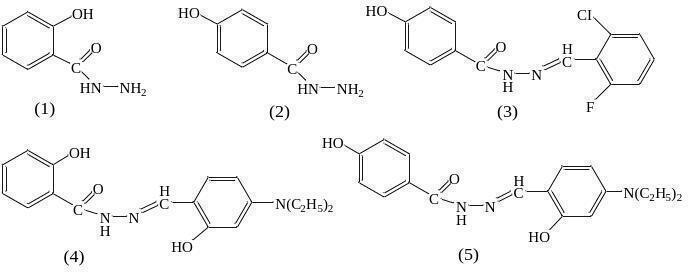
\includegraphics[width=0.8\textwidth]{assets/42}
	\caption*{}
\end{figure}

\begin{figure}[H]
	\centering
	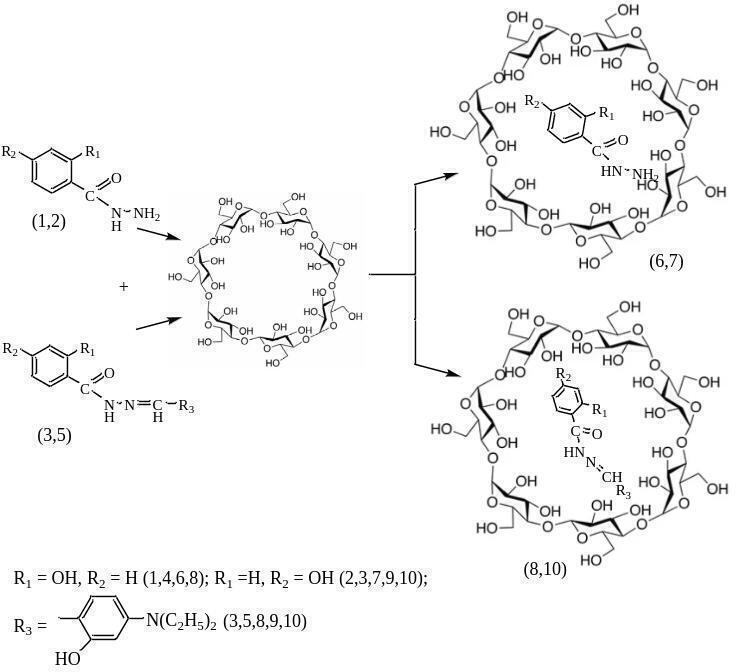
\includegraphics[width=0.8\textwidth]{assets/43}
	\caption*{}
\end{figure}

{\bfseries Рис. 1 -- Схема синтеза комплексов включений соединений (6-10)}

Комплексы включения гидразидов (1,2) и гидразонов (3-5) с ЦД-ном, а
также их комплексов (6-10) получали в виде кристаллических порошков
белого цвета с выходами 80-85\%. Конечные продукты были высушены в
сушильном шкафу при температуре 50±1°С. Полученные водорастворимые
комплексы включения гидразидов и их гидразоновые производные с ЦД-ном
(6-10) образуют устойчивые водные дисперсии, что приводит к повышению их
биологической доступности, тем самым сокращая их терапевтическую дозовую
концентрацию.

ИК спектры исходных и конечных продуктов регистрировали на спектрометре
с Фурье-преобразователем FSM 1201 по волновому числу в диапазоне от 4000
до 500 см\textsuperscript{-1} в таблетках с KBr. Спектры ЯМР
\textsuperscript{1}Н соединений снимали на спектрометре JNM-ECA Jeol 400
(частота 399.78 МГц) с использованием растворителей
ДМСО-d\textsubscript{6} и CDCl\textsubscript{3}. Химические сдвиги
измеряли относительно сигналов остаточных протонов или атомов углерода
дейтерированного растворителя. Температуры плавления определяли на
приборе «SMP10». Термогравиметрический (ТГ), дифференциальный
термический (ДТГ) и дифференциально-сканирующий калориметрический (ДСК)
анализ проводили на оборудовании ДТА/ДСК (Labsys EVO, Setaram, Франция)
в динамическом режиме в диапазоне температур 30-500°С при скорости
нагрева 100°С/мин в атмосфере азота и воздуха.

{\bfseries Результаты и обсуждение.} На рисунке 2 приведены ИК спектры ЦД
(а), физической смеси ЦД с (6) (б) и комплекса включения (6) (в).

\begin{figure}[H]
	\centering
	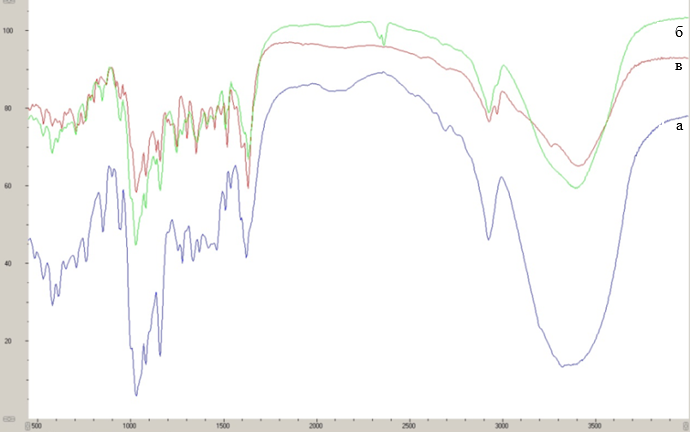
\includegraphics[width=0.8\textwidth]{assets/44}
	\caption*{}
\end{figure}

{\bfseries Рис. 2 -- ИК спектр ЦД (а), физической смеси ЦД и субстрата (б),
клатратного комплекса ЦД:(6) (в), соотношение (1:1)}

В ИК спектре полученного комплекса (6) ОН-группы ЦД проявляются широкой
характерной полосой в области 3310-3320 см\textsuperscript{-1},
колебания связи С-Н прописываются в областях 2900-2910 и 887-892
см\textsuperscript{-1}. Следует отметить, что в ИК спектрах всех
комплексов включений (6-10) основные характерные полосы поглощения
субстратов (1-5) не проявляются, так как это можно объяснить эффектом
экранирования широкими полосами поглощения функциональных групп ЦД.
Однако, в спектрах наблюдаются смещение характерных полос поглощения
комплексообразователя (молекулы полисахарида).

В таблице 1 приведены значения химического сдвигов Δδ протонов
комплексообразователя в ЯМР-\textsuperscript{1}Н спектрах ЦД и его
комплексе включения с продуктом (6) (2:1) в свободном состоянии
(δ\textsubscript{0}, м.д.) и в составе комплекса (δ, м.д.)

{\bfseries Таблица 1 -- Значения химического сдвигов Δδ протонов в
ЯМР-\textsuperscript{1}Н спектрах ЦД}

{\bfseries и его комплексе включения с продуктом (6) (2:1) в свободном
состоянии (δ\textsubscript{0}, м.д.)}

{\bfseries и в составе комплекса (δ, м.д.)}

\begin{longtable}[]{@{}
  >{\raggedright\arraybackslash}p{(\columnwidth - 6\tabcolsep) * \real{0.1235}}
  >{\raggedright\arraybackslash}p{(\columnwidth - 6\tabcolsep) * \real{0.2768}}
  >{\raggedright\arraybackslash}p{(\columnwidth - 6\tabcolsep) * \real{0.3075}}
  >{\raggedright\arraybackslash}p{(\columnwidth - 6\tabcolsep) * \real{0.2921}}@{}}
\toprule\noalign{}
\multirow{2}{=}{\begin{minipage}[b]{\linewidth}\raggedright
Протон
\end{minipage}} & \begin{minipage}[b]{\linewidth}\raggedright
δ\textsubscript{0}, м.д. (ЦД)
\end{minipage} & \begin{minipage}[b]{\linewidth}\raggedright
δ, м.д. (ЦД:(6))
\end{minipage} & \begin{minipage}[b]{\linewidth}\raggedright
Δδ (δ -- δ\textsubscript{0}), м.д.
\end{minipage} \\
& \begin{minipage}[b]{\linewidth}\raggedright
δ(\textsuperscript{1}Н)
\end{minipage} & \begin{minipage}[b]{\linewidth}\raggedright
δ(\textsuperscript{1}Н)
\end{minipage} & \begin{minipage}[b]{\linewidth}\raggedright
δ(\textsuperscript{1}Н)
\end{minipage} \\
\midrule\noalign{}
\endhead
\bottomrule\noalign{}
\endlastfoot
H1 & \multirow{6}{=}{4.77

3.26

3.43

3.27

3.43

3.58} & \multirow{6}{=}{4.76

3.28

3.35

3.26

3.37

3.59} & \multirow{6}{=}{-0.01

-0.02

-0.08

0.01

-0.06

0.01} \\
H2 \\
H3 \\
H4 \\
H5 \\
H6 \\
\end{longtable}

На основании приведенных в таблице 1 данных можно отметить, что
наибольшее смещение испытывают протоны внутренней сферы полисахарида --
Н3 и Н5. Эти данные свидетельствуют в пользу образования внутреннего
комплекса β-ЦД с (6) {[}9-12{]}.

На рисунке 3 показаны микрофотографии кристалликов комплексов, снятых
при различных увеличениях, на сканирующем электронном микроскопе, СЭМ -
β-ЦД, физической смеси ЦД и вещества (6) и комплекса включения ЦД:(6)
(2:1). Снимки (1-6) были сделаны при различных ускоряющих напряжениях.
На многократно увеличенных снимках комплексов наблюдается резкое
изменение морфологии и формы кристаллов: кристаллические формы частиц
клатратов имеют более сглаженный вид (возможно, из-за пленкообразования
(снимки 5 и 6) при SEM MAG 69,2kx). Изменения морфологии поверхности
кристаллов при комплексообразовании субстрата с молекулой полисахарида
являются одним из доказательств образования комплексов включений.

% \begin{longtable}[]{@{}
%   >{\raggedright\arraybackslash}p{(\columnwidth - 4\tabcolsep) * \real{0.3399}}
%   >{\raggedright\arraybackslash}p{(\columnwidth - 4\tabcolsep) * \real{0.3284}}
%   >{\raggedright\arraybackslash}p{(\columnwidth - 4\tabcolsep) * \real{0.3317}}@{}}
% \toprule\noalign{}
% \begin{minipage}[b]{\linewidth}\raggedright
% \begin{figure}[H]
% 	\centering
% 	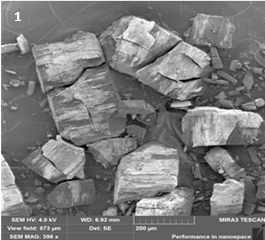
\includegraphics[width=0.8\textwidth]{assets/45}
% 	\caption*{}
% \end{figure}
% \end{minipage} & \begin{minipage}[b]{\linewidth}\raggedright
% \begin{figure}[H]
% 	\centering
% 	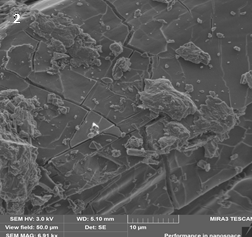
\includegraphics[width=0.8\textwidth]{assets/46}
% 	\caption*{}
% \end{figure}
% \end{minipage} & \begin{minipage}[b]{\linewidth}\raggedright
% \begin{figure}[H]
% 	\centering
% 	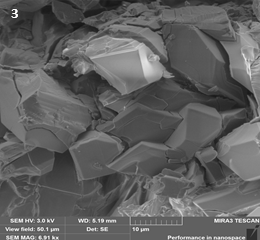
\includegraphics[width=0.8\textwidth]{assets/47}
% 	\caption*{}
% \end{figure}
% \end{minipage} \\
% \midrule\noalign{}
% \endhead
% \bottomrule\noalign{}
% \endlastfoot
% \begin{figure}[H]
% 	\centering
% 	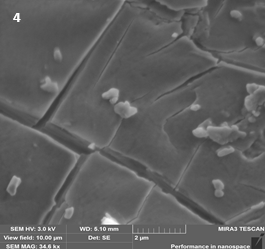
\includegraphics[width=0.8\textwidth]{assets/48}
% 	\caption*{}
% \end{figure} &
% \begin{figure}[H]
% 	\centering
% 	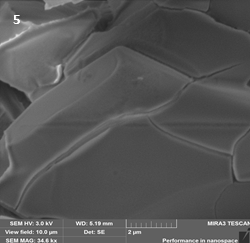
\includegraphics[width=0.8\textwidth]{assets/49}
% 	\caption*{}
% \end{figure} &
% \begin{figure}[H]
% 	\centering
% 	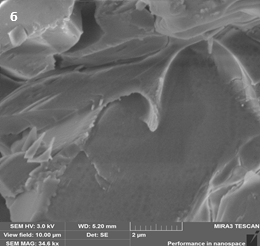
\includegraphics[width=0.8\textwidth]{assets/50}
% 	\caption*{}
% \end{figure} \\
% \end{longtable}

{\bfseries Рис. 3 - Электронные микрофотографии ЦД (снимки 1, 2),
физической смеси ЦД с (6) (снимки 3,4) и комплекса ЦД:(6) (2:1) (снимки
при различных увеличениях)}

Термическую стабильность полученных комплексов включения гидразидов и их
гидразоновых производных при комплексообразовании с ЦД изучали с помощью
диференциального термического анализа (ДТА). С помошью метода
дифференциальной сканирующей калориметрии можно установить зависимость
изменение массы синтезированных супрамолекулярных комплексов включения
от температуры (термогравиметрическая кривая) и по ее пику точно
определить максимальную скорость горения комплекса {[}13{]}.

На рисунках 4 и 5 приведены TГ/ДТА кривые ЦД и физической смеси ЦД с (6)
и комплекса включения ЦД:(6). Согласно данным TГ в интервале температур
от 32,8°С до 320°С циклодекстриновый комплекс включения ЦД:(6) не
претерпевает превращений, приводящих к изменению его массы {[}14,15{]}.
Основное количество летучих компонентов выделилось при 330°С-370°С. В
этом интервале происходит интенсивная убыль массы комплекса, о чем
свидетельствует ход термогравиметрической кривой. Процесс деструкции
практический полностью завершается при температуре 380°С.

\begin{figure}[H]
	\centering
	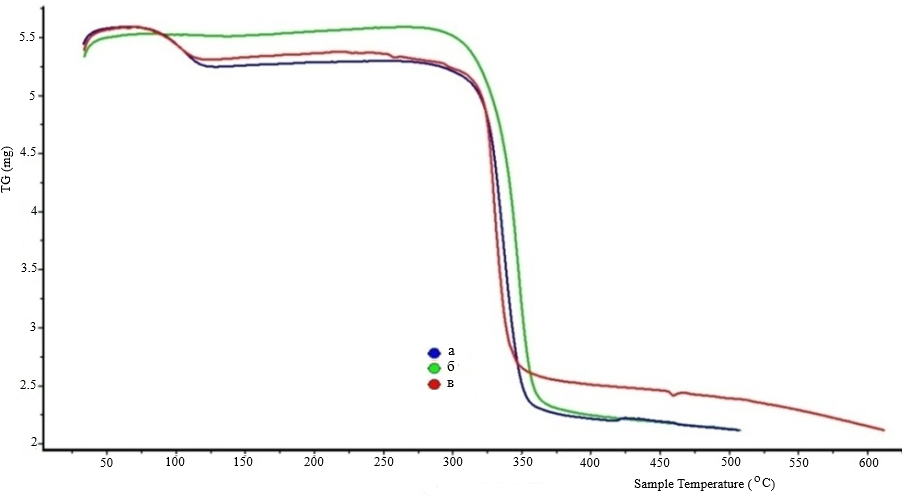
\includegraphics[width=0.8\textwidth]{assets/51}
	\caption*{}
\end{figure}

{\bfseries Рис. 4 - Термогравиметрические кривые циклодекстрина (а),
продукта (6) и комплекса включения ЦД:(6)}

\begin{figure}[H]
	\centering
	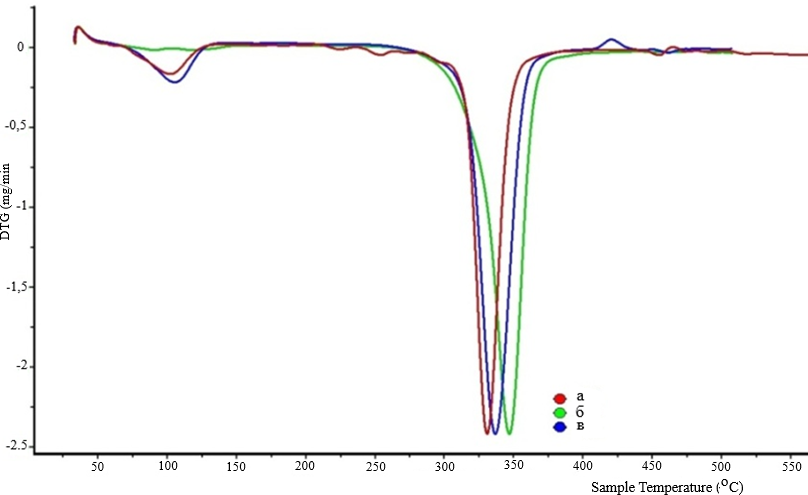
\includegraphics[width=0.8\textwidth]{assets/52}
	\caption*{}
\end{figure}

{\bfseries Рис. 5 -- Дифференциальная сканирующая калориметрия комплекса
включения ЦД:(6) (а), физической смеси ЦД:(6) (б) (соотношение (1:1) и
циклодекстрина (в)}

Синтезированные комплексы включения содержали воду, которому
свидетельствуют эндотермический пик дегидратации в диапазоне 50-125°С,
это является переходом ЦД в безводную форму в результате испарения воды
{[}14,15{]}. Процесс термодеструкции ЦД начинается с 300°С, в области
температур 329-348°С происходит термодеструкция комплекса включения, что
свидетельствует о повышении термостабильности ЦД при включении в его
полость биологически активного компонента (6). На кривой скорости потери
массы в интервале температур 32°С-270°С не наблюдается изменение
скорости. Начиная с 310°С наблюдается резкое увеличение скорости и
достигает своего пика при ≈ 340°С, значение скорости при данной
температуре составляет 1,7 мг/мин. Далее идет постепенное уменьшение, и
при 380°С скорость стабилизируется. На кривой ДСК при температуре 329°С
(9), 335°С (8), 348\textsuperscript{0}С (10) наблюдается эндотермический
пик, обусловленный плавлением, при этом масса вещества не меняется,
далее при температуре ≈ 370°С присутствует экзотермический эффект,
которое объясняется разложением образца с выделением летучих продуктов и
потерей массы.

{\bfseries Выводы.} В химической фармакологии используются различные пути
повышения растворимости биоактивных веществ с использованием специальных
макромолекулярных биополимеров - краун-эфиров, криптандов, циклофанов,
каликсаренов, хитазана и полисахаридов как комплексообразователей.
Получением комплексов включения можно увеличить растворимость и
стабильность низкомолекулярных веществ. Гидразиды \emph{о}- и \emph{п}-
гидроксибензойных кислот и их гидразоновые производные могут
образовывать различные комплексы включений с макромолекулярными
биополимерами. Полученные продукты образуют смесь, способных
растворяться в воде или образовывать устойчивые водные дисперсии.
Получение водорастворимых комплексов указанных соединений должно
привести к повышению их биологической доступности, что соответственно
позволит значительно сократить их терапевтическую концентрацию. Данные
физико-химических методов исследований (ИК-, ЯМР \textsuperscript{1}Н
спектры, ДТГ, СЭМ) могут быть использованы при анализе полученных
комплексов включений биоактивных веществ.

\emph{{\bfseries Финансирование:} Научно-исследовательская работа
осуществлена в рамках ГФ АР14869941 Комитета науки Министерства науки и
высшего образования Республики Казахстан.}

{\bfseries Литература}

1. Лисина С.В., Брель А.К., Мазанова Л.С., Спасов А.А. Синтез и
жаропонижающая активность новых производных салициловой
кислоты//Химико-фармацевтический журнал.- 2008.-Т.42.(10).- С.24-26. DOI
10.30906/0023-1134-2008-42-10-24-26

2. Беликов В.Г. Синтетические и природные лекарственные средства. - М.:
Высшая школа. - 1993. - 720 с. ISBN 5-06-002985-9

3. Машковский М.Д. Лекарственные средства. -- М.: ООО РИА «Новая волна».
- 2012. -- 1216 с. ISBN 978-5-7864-0218-7

4. Степаненко Б.Н. Химия и биохимия углеводов: моносахариды. -- М.:
Высш. Школа. - 1977. -- 223 с.

5. Szejtli J. Cyclodextrin Technology. Dordrecht, Netherlands: Kluwer
Academic Publishers. - 1988.- 450 p. ISBN 9789027723147

6. Nurkenov O.A., Fazylov S.D., Satpaeva Zh.B., Seilkhanov T.M.,
Turdybekov D.M., Mendibayeva A.Zh., Akhmetova S.B, Shulgau Z.T.,
Alkhimova L.E., Kulakov I.V. Synthesis, structure and biological
activity of hydrazones derived from 2- and 4-hydroxybenzoic acid
hydrazides // Chemical Data Collections.-2023.-Vol.48,Article101089.

DOI 10.1016/j.cdc.2023.101089.

7. Miranda J.C. Cyclodextrins and ternary complexes technology to
improve solubility of poorly soluble drugs // Brazilian Journal of
Pharmaceutical Sciences.-- 2011.-- Vol. 47(4). -- Р. 665-681.

DOI 10.1590/S1984-82502011000400003

8. Dodzink H. Cyclodextrins and their complexes: Chemistry, analytical
methods, applications. -- Weinheim:Willey-VCH.- 2006.-504 p. ISBN:
978-3-527-60844-7

9. Crini G. Review: A history of cyclodextrins // Chemical Reviews.-
2014.-Vol. 114(21).-Р. 10940-10975. DOI 10.1021/cr500081p

10. Bary A.R., Tucker I.G., Davies N.M. Considerations in the use of
hydroxypropyl-beta-cyclodextrin in the formulation of aqueous ophthalmic
solutions of hydrocortisone // European Journal of Pharmaceutics and
Biopharmaceutics.- 2000.-Vol. 50(2).- Р. 237-244.

DOI 10.1016/s0939-6411(00)00108-9

11. Krzysztof C., Centkowska K. Use of cyclodextrins in topical
formulations: Practical aspects // European Journal of Pharmaceutical
and Biopharmaceutics.- 2008. -Vol. 68.- Р.467-478.

DOI 10.1016/j.ejpb.2007.08.002

12. Wuthrich K., Billeter M., Gurtert P., Luginbuhl P., Riek R., Wider
G. NMR studies of the hydration of biological macromolecules // Faraday
Discuss. -1996. - Vol.103. - Р.245-253.

DOI 10.1039/FD9960300245

13. Castronuovo G., Niccoli M. Thermodynamics of inclusion complexes of
natural and modified cyclodextrins with acetylsalicylic acid and
ibuprofen in aqueous solution at 298 K // Thermochimica Acta. - 2013.-
Vol. 557. - Р. 44 - 49. DOI10.1016/j.tca.2013.01.037

14. Сastronuovo G., Niccoli M. Thermodynamics of inclusion complexes of
natural and modified cyclodextrins with propranolol in aqueous solution
at 298 K // Bioorganic and Medical Chemistry. -2006.-Vol.14(11)-
Р.3883-3887. DOI 10.1016/j.bmc.2006.01.052~

15. Qvist J., Halle B. Thermal signature of hydrophobic hydration
dinamics // American Chemical Society. -2008. - Vol.130(31) -
Р.10345-10353. DOI 10.1021/ja802668w

{\bfseries References}

1. Lisina S.V., Brel\textquotesingle{} A.K., Mazanova L.S., Spasov A.A.
Sintez i zharoponizhajushhaja aktivnost\textquotesingle{} novyh
proizvodnyh salicilovoj kisloty//Himiko-farmacevticheskij zhurnal.-
2008.-T.42.(10).- S.24-26. DOI 10.30906/0023-1134-2008-42-10-24-26 {[}in
Russ.{]}

2. Belikov V.G. Sinteticheskie i prirodnye lekarstvennye sredstva. - M.:
Vysshaja shkola. - 1993. - 720 s. ISBN 5-06-002985-9. {[}in Russ.{]}

3. Mashkovskij M.D. Lekarstvennye sredstva. -- M.: OOO RIA «Novaja
volna». - 2012. -- 1216 s. ISBN 978-5-7864-0218-7. {[}in Russ.{]}

4. Stepanenko B.N. Himija i biohimija uglevodov: monosaharidy.-
M.:Vyssh. Shkola. - 1977.- 223 s. {[}in Russ.{]}

5. Szejtli J. Cyclodextrin Technology. Dordrecht, Netherlands: Kluwer
Academic Publishers. - 1988.- 450 p. ISBN 9789027723147

6. Nurkenov O.A., Fazylov S.D., Satpaeva Zh.B., Seilkhanov T.M.,
Turdybekov D.M., Mendibayeva A.Zh., Akhmetova S.B, Shulgau Z.T.,
Alkhimova L.E., Kulakov I.V. Synthesis, structure and biological
activity of hydrazones derived from 2- and 4-hydroxybenzoic acid
hydrazides // Chemical Data Collections.-2023.-Vol.48,Article101089.

DOI 10.1016/j.cdc.2023.101089.

7. Miranda J.C. Cyclodextrins and ternary complexes technology to
improve solubility of poorly soluble drugs // Brazilian Journal of
Pharmaceutical Sciences.-- 2011.-- Vol. 47(4). -- Р. 665-681.

DOI 10.1590/S1984-82502011000400003

8. Dodzink H. Cyclodextrins and their complexes: Chemistry, analytical
methods, applications. -- Weinheim:Willey-VCH.- 2006.-504 p. ISBN:
978-3-527-60844-7

9. Crini G. Review: A history of cyclodextrins // Chemical Reviews.-
2014.-Vol. 114(21).-Р. 10940-10975. DOI 10.1021/cr500081p

10. Bary A.R., Tucker I.G., Davies N.M. Considerations in the use of
hydroxypropyl-beta-cyclodextrin in the formulation of aqueous ophthalmic
solutions of hydrocortisone // European Journal of Pharmaceutics and
Biopharmaceutics.- 2000.-Vol. 50(2).- Р. 237-244.

DOI 10.1016/s0939-6411(00)00108-9

11. Krzysztof C., Centkowska K. Use of cyclodextrins in topical
formulations: Practical aspects // European Journal of Pharmaceutical
and Biopharmaceutics.- 2008. -Vol. 68.- Р.467-478.

DOI 10.1016/j.ejpb.2007.08.002

12. Wuthrich K., Billeter M., Gurtert P., Luginbuhl P., Riek R., Wider
G. NMR studies of the hydration of biological macromolecules // Faraday
Discuss. -1996. - Vol.103. - Р.245-253.

DOI 10.1039/FD9960300245

13. Castronuovo G., Niccoli M. Thermodynamics of inclusion complexes of
natural and modified cyclodextrins with acetylsalicylic acid and
ibuprofen in aqueous solution at 298 K // Thermochimica Acta. - 2013.-
Vol. 557. - Р. 44 - 49. DOI10.1016/j.tca.2013.01.037

14. Сastronuovo G., Niccoli M. Thermodynamics of inclusion complexes of
natural and modified cyclodextrins with propranolol in aqueous solution
at 298 K // Bioorganic and Medical Chemistry. -2006.-Vol.14(11)-
Р.3883-3887. DOI 10.1016/j.bmc.2006.01.052~

15. Qvist J., Halle B. Thermal signature of hydrophobic hydration
dinamics // American Chemical Society. -2008. - Vol.130(31) -
Р.10345-10353. DOI 10.1021/ja802668w

\emph{{\bfseries Сведения об авторах}}

Фазылов С.Д{\bfseries .} (автор-корреспондент)- академик НАН РК, доктор
химических наук, профессор, главный научный сотрудник Института
органического синтеза и углехимии Республики Казахстан, Караганда,
Казахстан, e-mail: iosu8990@mail.ru;

Сатпаева Ж.Б. -старший преподаватель кафедры органической химии и
полимеров Карагандинского университета им. Е.А. Букетова, e-mail:
satpaeva\_zh@mail.ru;

Нуркенов О.А.-доктор химических наук, профессор, заведующий лабораторией
Синтез биологически активных веществ Института органического синтеза и
углехимии Республики Казахстан, Караганда, Казахстан; e-mail:
nurkenov\_oral@mail.ru;

Бакирова Р.Е.- доктор медицинских наук, профессор кафедры внутренних
болезней Медицинского университета Караганды, Караганда, Казахстан,
e-mail: bakir15@mail.ru;

Свидерский А.К.-доктор химических наук, профессор Жезказганского
университета им. О.А.Байконурова, Жезказган, Казахстан, e-mail:
katsostud@rambler.ru;

Мендибаева А.Ж{\bfseries .} - младший научный сотрудник Института
органического синтеза и углехимии Республики Казахстан, Караганда,
Казахстан; e-mail: anenyawa@mail.ru

\emph{{\bfseries Information about the author}}

Fazylov S.D.(Corresponding author) - Academician of the National Academy
of Sciences of the Republic of Kazakhstan, Doctor of Chemical Sciences,
Professor, Chief Scientific Associate of the Institute of Organic
Synthesis and Coal Chemistry of the Republic of Kazakhstan, Karaganda,
Kazakhstan, е-mail: iosu8990@mail.ru;

Satpaeva Zh. - Senior Lecturer of the Department of Organic Chemistry
and Polymers, Karaganda University named after Academician E.A.Buketov,
Karaganda, Kazakhstan, e-mail: satpaeva\_zh@mail.ru;

Nurkenov O.A. - Doctor of Chemical Sciences, Professor, Head of the
Laboratory of Synthesis of Biologically Active Substances of the
Institute of Organic Synthesis and Coal Chemistry of the Republic of
Kazakhstan, Karaganda, Kazakhstan, е-mail: nurkenov\_oral@mail.ru;

Bakirova R.E. - Doctor of Medical Sciences, Professor of Internal
Medicine Department, Medical University of Karaganda, Karaganda,
Kazakhstan, e-mail: bakir15@mail.ru;

Sviderskyi A.К. - Doctor of Chemical Sciences, Professor of the
O.A.Baikonurov Zhezkazgan University, Zhezkazgan, Kazakhstan, e-mail:
katsostud@rambler.ru;

Mendibayeva A.Zh. - Junior researcher, LLP ``Institute of Organic
Synthesis and Coal Chemistry of the Republic of Kazakhstan'', Karaganda,
Kazakhstan; е-mail: anenyawa@mail.ru\newpage
{\bfseries IRSTI 61.31.40}

{\bfseries OBTAINING CARBON NANOMATERIALS FROM SHUBARKOL COAL AND
APPLICATION FOR HYDROGEN STORAGE}

{\bfseries \textsuperscript{1,2,3}M.K. Kazankapova,
\textsuperscript{1,2}B.T. Yermagambet, \textsuperscript{1,2}G.K.
Mendaliyev, \textsuperscript{1}A. Samatkyzy, \textsuperscript{1,2}A.B.
Malgazhdarova}

\textsuperscript{1}«Institute of Coal Chemistry and Technology» LLP,
Astana, Kazakhstan,

\textsuperscript{2}L.N. Gumilyov Eurasian National University{\bfseries ,}
Astana, Kazakhstan,

\textsuperscript{3}Kazakh university of technology and business named
after K. Kulazhanov, Astana, Kazakhstan

Corresponding author: е-mail: coaltech@bk.ru

This study presents a promising method for the synthesis of graphene -
the electric arc discharge method. The synthesis of nanomaterials
containing graphene was carried out based on carbonized coal "Shubarkol"
using the electric arc discharge method at a constant voltage of 75 V
and a current of 100 A in a quartz reactor. Based on Raman scattering
data and analysis of electrical properties (dielectric constant and
electrical resistance), it was shown that the synthesized products have
a high degree of graphitization and long-range structural order (2D
peak), which indicates the formation of nanomaterials containing
graphene. These results present a potential route for low-cost mass
production of high-quality graphene samples. In addition, the electrical
resistance (R), capacitance (C) and dielectric constant (ε), electrical
resistivity (R) and electrical conductivity (χ) of nanomaterials
containing graphene were determined for the first time in the
temperature range 293-483 K. The highest a degree of graphitization of
80.7\% is achieved with the formation of graphene-containing material on
the walls of the reactor after an arc discharge. Since the resulting
nanomaterial on the reactor walls showed better results in terms of
physicochemical and electrophysical properties, the material was tested
for hydrogen storage. The sorption capacity of the nanomaterial for
hydrogen was 35.1516 cm\textsuperscript{3}/g (0.314\%).

{\bfseries Key words:} coal, carbonized coal, carbon nanotubes, graphene,
arc discharge, hydrogen, storage.

{\bfseries ШҰБАРКӨЛ КӨМІРІНЕН КӨМІРТЕК НАНОМАТЕРИАЛДАРЫН АЛУ ЖӘНЕ СУТЕКТІ
САҚТАУҒА ҚОЛДАНУ}

{\bfseries \textsuperscript{1,2,3}М.Қ. Қазанқапова,
\textsuperscript{1,2}Б.Т. Ермағамбет, \textsuperscript{1,2}Ғ.К.
Мендалиев, \textsuperscript{1}Ә. Саматқызы,}

{\bfseries \textsuperscript{1,2}А.Б.Малғаждарова}

\textsuperscript{1}«Көмір химиясы және технология институты» ЖШС,
Астана, Қазақстан,

\textsuperscript{2}Л.Н. Гумилев атындағы Еуразия ұлттық университеті,
Астана, Қазақстан,

\textsuperscript{3}Қ.Құлажанов атындағы Қазақ технология және бизнес
университеті, Астана, Қазақстан,

е-mail: coaltech@bk.ru

Бұл зерттеуде графен синтезінің перспективті әдісі - электр доғалық
разряд әдісі ұсынылды. Құрамында графен бар наноматериалдардың синтезі
кварц реакторында 75 В тұрақты кернеуде және 100 А ток кезінде электр
доғалық разряд әдісін қолдану арқылы «Шұбаркөл» көмірі негізінде жүзеге
асырылды. Раман шашырау деректері және электрлік қасиеттерді талдау
(диэлектрлік өтімділік және электр кедергісі) негізінде синтезделген
өнімдерде графиттенудің жоғары дәрежесі және алысдиапазондағы құрылымдық
реті (2D шыңы) бар, бұл құрамында графен бар наноматериалдардың түзілуін
көрсетеді. Бұл нәтижелер жоғары сапалы графен үлгілерін арзан жаппай
өндірудің әлеуетті бағытын көрсетеді. Сонымен қатар, құрамында графен
бар наноматериалдардың электрлік кедергісі (R), сыйымдылығы (C) және
диэлектрлік өтімділігі (ε), электрлік кедергісі (R) және электр
өткізгіштігі (χ) 293-483 К температура диапазонында алғаш рет анықталды.
Графиттенудің ең жоғары дәрежесі 80,7\% доғалық разрядтан кейін
реактордың қабырғаларында графен бар материалдың пайда болуымен қол
жеткізіледі. Реактор қабырғаларында алынған наноматериал физика-химиялық
және электрофизикалық қасиеттері бойынша жақсы нәтиже көрсеткендіктен,
материал сутегі сақтау үшін сынақтан өтті. Наноматериалдың сутегі үшін
сорбциялық қабілеті 35,1516 см\textsuperscript{3}/г (0,314\%) құрады.

{\bfseries Түйін сөздер:} көмір, көміртекті көмір, көміртекті нанотүтіктер,
графен, доғалық разряд, сутегі, сақтау.

{\bfseries ПОЛУЧЕНИЕ УГЛЕРОДНЫХ НАНОМАТЕРИАЛОВ ИЗ ШУБАРКОЛЬСКОГО УГЛЯ И
ПРИМЕНЕНИЕ ДЛЯ ХРАНЕНИЯ ВОДОРОДА}

{\bfseries \textsuperscript{1,2,3}М.К. Казанкапова,
\textsuperscript{1,2}Б.Т. Ермағамбет, \textsuperscript{1,2}Г.К.
Мендалиев, \textsuperscript{1}А. Саматкызы, \textsuperscript{1,2}Б А.Б.
Малгаждарова}

\textsuperscript{1}ТОО «Институт химии угля и технологии», Астана,
Казахстан,

\textsuperscript{2}Евразийский национальный университет им. Л.Н.
Гумилева, Астана, Казахстан,

\textsuperscript{3}Казахский университет технологии и бизнеса имени
К.Кулажанова, Астана, Казахстан,

е-mail: coaltech@bk.ru

В данном исследовании представлен перспективный метод синтеза графена -
метод электродугового разряда. Был осуществлен синтез наноматериалов,
содержащих графен, на основе карбонизованного угля «Шубарколь» с
использованием метода электродугового разряда при постоянном напряжении
75 В и токе 100 А в кварцевом реакторе. На основе данных метода
комбинационного рассеяния света и анализа электрофизических свойств
(диэлектрической проницаемости и электрического сопротивления) было
показано, что синтезированные продукты обладают высокой степенью
графитизации и дальним порядком структуры (2D пик), что свидетельствует
о формировании наноматериалов, содержащих графен. Эти результаты
представляют потенциальный путь для дешевого массового производства
высококачественных образцов графена. Кроме того, впервые были определены
электрическое сопротивление (R), емкость (C) и диэлектрическая
проницаемость (ε), удельное электрическое сопротивление (R) и удельная
электропроводность (χ) наноматериалов, содержащих графен, в интервале
температур 293-483 К. Самая высокая степень графитизации 80,7\%
достигается при образовании графенсодержащего материала на стенках
реактора после дугового разряда. Поскольку полученный наноматериал на
стенках реактора показал лучшие результаты по физико-химическим и
электрофизическим свойствам, материал был протестирован на хранение
водорода. Сорбционная емкость наноматриала по водороду составила -
35.1516 см\textsuperscript{3}/г (0.314\%).

{\bfseries Ключевые слова:} уголь, карбонизованный уголь, углеродные
нанотрубки, графен, дуговой разряд, водород, хранение.

{\bfseries Introduction.} Since Sumio Iijima reported it in 1991, carbon
nanotubes (CNTs) have attracted much attention from researchers and
industry. CNTs can be classified into single-walled CNTs (SWNTs),
double-walled CNTs (DWNTs), and multi-walled CNTs (MWNTs) depending on
the number of graphite layers. They consist of sp\textsuperscript{2}
bonded carbon atoms arranged in a cylindrical tube ranging in length
from less than 100 nm to several centimeters. The diameter of SWCNTs is
typically 0.4--2 nm, while the diameter of MWCNTs ranges from *1.4 nm to
nearly 100 nm, depending on the synthesis conditions. CNTs are well
known for their unique physicochemical properties, including extremely
high tensile strength, high electrical conductivity, high ductility, and
relative chemical inactivity. All these properties make CNT-based
products attractive. Moreover, due to their low dimensionality, CNTs are
also preferred for use in the development of nanocomposites. In this
context, CNTs open up a new direction in materials science and
nanotechnology. CNTs can be found in a wide range of applications, such
as electronics, polymer composites, energy storage materials, catalysis,
gas storage materials and sensors {[}1{]}.

There are many methods for synthesizing nanostructures. They are usually
divided into two groups: «Top bottom» is a «top-down» technology, that
is, the dispersion of macroscopic bodies into nanoscale sizes, and the
second group «bottom-up» is a technology the assembly of nanoparticles
from atoms. There are also various hybrid methods.

One of the first methods for producing carbon nanoparticles was laser
evaporation of graphite or coal, arc evaporation of graphite in the
presence of a metal catalyst, chemical vapor deposition, pyrolysis, and
mechanical separation {[}2{]}.

Arc discharge is the oldest and most common method for producing CNM.
This also makes it possible to obtain carbon formed by fullerene and
soot molecules. This method is based on the electrical destruction of
gas to produce plasma. It uses high temperature (over 1700°C) to
evaporate carbon atoms in plasma, allowing CNMs to grow with fewer
structural defects than other methods.

The chamber consists of two electrodes, one of which is the anode and
the other is the cathode. The anode is filled with a mixture of graphite
powder and catalyst. The catalyst promotes the growth of SWCNTs rather
than MWCNTs {[}3{]}. The cathode consists of a pure graphite rod.
Initially, the electrodes are held independently of each other in a gas
atmosphere (usually an argon/hydrogen mixture); then the distance
between the electrodes is reduced, and an electric arc is applied with
an intensity of 60-100 A or 50-150 A, which corresponds to a decrease in
potential by 25 V {[}4, 5{]}.

The inert gas flow is maintained at 50-600 Torr; the temperature in the
interelectrode region ranges from 1700° to 4000 °C. The electrodes turn
red and plasma is formed, so carbon sublimes from the positive anode,
which is consumed and condenses as a filamentary carbon product at the
cathode due to the temperature gradient.

Speaking about the physical and chemical properties of carbon nanotubes,
CNTs are the strongest and hardest materials on earth in terms of
tensile strength and elastic modulus. The planar cellular carbon atoms
of graphene in CNTs are responsible for these high-strength fibers.
Carbon nanotube is more rigid than steel and is very resistant to
physical damage.

When you press on the end of the nanotube, it bends without damaging the
tip, and when the force is removed, the tip returns to its original
position. The reason they don\textquotesingle t break is because the
carbon rings of the walls change their structure when bent, but
don\textquotesingle t break. This is a unique result of sp2 C-C bond
hybridization and bending overhybridization. The degree of change and
s-p coefficients depend on how much the bonds bend. Due to this
property, CNTs can be used as very high resolution probe tips for
scanning probe microscopy {[}6{]}.

In the metallic state, the conductivity of nanotubes is very high. They
can transmit billions of amps per square centimeter. Copper wire fails
when it transmits a million amps per square centimeter because the
joules of heat cause the wire to melt. Theoretically, metal nanotubes
can conduct an electric current density of 10-15
A/cm\textsuperscript{2}, which is 1000 times greater than that of metals
such as copper {[}7{]}. One of the reasons for the high conductivity of
carbon nanotubes is the very small number of defects that cause electron
scattering and therefore low resistance {[}8{]}.

Another carbon nanomaterial that can be synthesized by an arc discharge
is graphene {[}9-10{]}. Graphene is a material that has a large specific
surface area (2630 m2g-1), high internal mobility (200,000
cm\textsuperscript{2} V\textsuperscript{-1}s\textsuperscript{-1}), high
Young\textquotesingle s modulus (\textasciitilde{} 1.0 TPa), thermal
conductivity (\textasciitilde5000
W*m\textsuperscript{-1}/K\textsuperscript{-1}), optical transmittance
(\textasciitilde{} 97.7\%) {[}11-12{]}. In addition to arc, there are
methods of micromechanical cleavage, electrochemical exfoliation,
solvent-based exfoliation {[}13{]}, graphite oxide exfoliation {[}14{]}
and laser evaporation. Among all these methods, arc discharge has many
advantages such as low production cost, high efficiency, and the ability
to be synthesized without using any catalysis {[}15{]}.

In the research, multiple layers of graphene were synthesized using a
homemade arc discharge chamber. Helium (He), nitrogen (N), and mixtures
thereof have been used to understand the influence of the reactor
atmosphere on graphene synthesis. The purity and number of graphene
layers were determined using Raman spectroscopy. The purity of the
synthesized graphene also depends on the diameter of the electrodes and
the arc current. Thus, optimal synthesis conditions were obtained with
an electrode diameter of 12 mm and an arc current of 150 A in a
He+N\textsubscript{2} atmosphere. TEM studies revealed a crumpled
texture of graphene {[}16{]}.

Graphene can be doped with atoms of other elements, such as nitrogen,
fluorine, hydrogen, oxygen, etc., changing its properties. All this
makes it an interesting material for many applications. First of all,
these are applications in opto- and nanoelectronics (touch screens,
solar cells, flexible electronic devices, high-frequency transistors,
logic transistors), photonics (photodetectors, optical modulators,
mode-locked lasers, THz generators and optical polarizers), composite
materials, paints and coatings. Graphene is seen as a promising
candidate to replace transparent indium tin oxide (ITO) electrodes.
Promising applications of graphene coating include transparent heating
elements and thermoacoustic transducers.

{\bfseries Materials and methods.} In this work, carbon nanomaterials
obtained by the electric arc method were studied. Activated carbon
«Shubarkol» is used as an electrode. The coal carbonization process
includes an initial low-temperature (at 180°C, with a heating rate of
10°C/min) treatment of the raw material in the presence of air for 1
hour, followed by carbonization in an inert atmosphere at temperatures
ranging from 180-900°C with a heating rate of 5°C/min, and steam
activation at the maximum temperature for 1 hour. Process parameters:
constant voltage - 75 V; current -- \hspace{0pt}\hspace{0pt}100 A;
process time \textasciitilde10 min, inert gas - N\textsubscript{2} with
a purity of 99.99\%. The reactor is transparent quartz glass that can
withstand high temperatures. The chamber is placed inside the water used
for cooling. The principle of this method is the evaporation of carbon
under reduced pressure of an inert gas. According to the method scheme,
a movable anode and a stationary cathode are used, as in Fig. 1.

\begin{figure}[H]
	\centering
	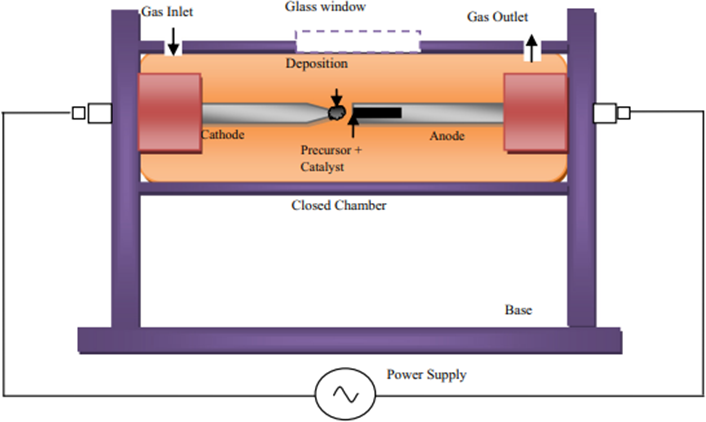
\includegraphics[width=0.8\textwidth]{assets/53}
	\caption*{}
\end{figure}

{\bfseries Figure 1 - Schematic diagram of an electric arc discharge}

After the electric arc is ignited, the plasma ignites. Carbon
nanomaterials condensed on the walls of the reactor and on the surface
of the electrode. Activated carbon "Shubarkol" after an arc discharge
was separated according to figure 2.

\begin{figure}[H]
	\centering
	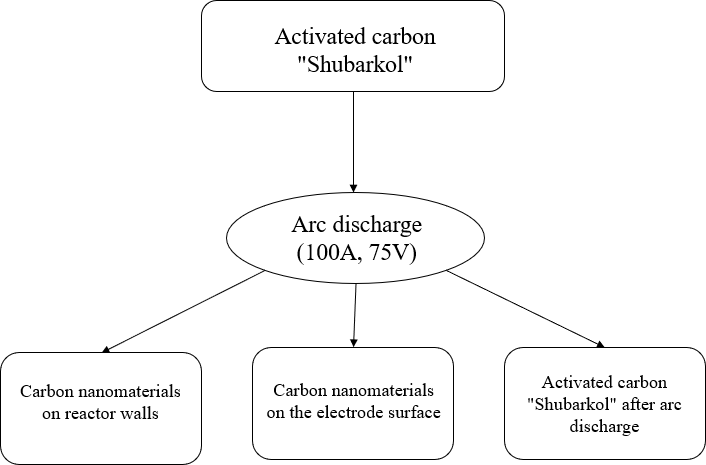
\includegraphics[width=0.8\textwidth]{assets/54}
	\caption*{}
\end{figure}

{\bfseries Figure 2 - Schematic diagram for producing nanomaterials using
the electric arc discharge method}

The resulting materials were tested for hydrogen storage at a
high-performance automatic physiosorption and chemisorption station
Micromeritics 3Flex Chemi\&TCD (Made in the USA). This device is
equipped with three ports, each of which has a 0.1 Torr sensor for
analysis of micropores. Before measurement, all samples were
preliminarily degassed using a SmartVacPrep unit (manufactured by
Micromeritics, USA) equipped with a forevacuum pump.

Adsorbate gas - hydrogen, measurement temperature - 77 K,
p\textsubscript{0} values \hspace{0pt}\hspace{0pt}for all points were
considered the same and equal to 760 Torr, A Peak Scientific hydrogen
generator with a maximum productivity of 500 cm\textsuperscript{3}/min
was used as a source of hydrogen, Water in the hydrogen generator was
used from a Thermo Scientific deionizer, Readout points started from a
value of 0.0001 p/p\textsubscript{0} to 0.995 p/p\textsubscript{0}. The
measurement of free space or void volume was carried out after analysis
with helium in order to avoid premature filling of micropores with
helium.

Due to the smaller radius and transverse radius of the hydrogen
molecule, the specific surface area and porosity values
\hspace{0pt}\hspace{0pt}will be higher compared to nitrogen sorption.
Classical BET methods in the case of H\textsubscript{2} will be
incorrect since the saturation pressure value was used as a constant
(760 Torr). To calculate the pore distribution, the theoretical hydrogen
sorption model DFT HS H\textsubscript{2} Carbon, heterogeneous, taking
into account the heterogeneity of the carbon surface. For most samples,
this model showed good consistency. The limitation of nitrogen to fill
pores with a radius of less than 0.35 nm was also taken into account.

{\bfseries Results and discussion.} The obtained materials were studied by
SEM and Raman spectroscopy. As a result, the original «Shubarkol» coal
contained different agglomerates ranging from 719 nm to 231.97 µm, as
shown in Fig. 3. The degree of graphitization is G\textsubscript{f} =
29.6\% and peaks at 1258.3 are noticeable; 1374.9; 1535.1; 1594.3;
2704.9; 2928.6 cm\textsuperscript{-1}. I(D)/I(G)=0.6 I(G)/I(2D)=12.2.
The intensity of peak D at 1374.9 cm\textsuperscript{-1} is lower than
peak G at 1594.3 cm\textsuperscript{-1}, and peak G at 1594.3
cm\textsuperscript{-1} is much higher than peak 2D at 2704.9
cm\textsuperscript{-1} (Figure 4), this explains that the material is
amorphous carbon. There may be polymer chains or other impurities, as
indicated by the luminescent trend.

\begin{figure}[H]
	\centering
	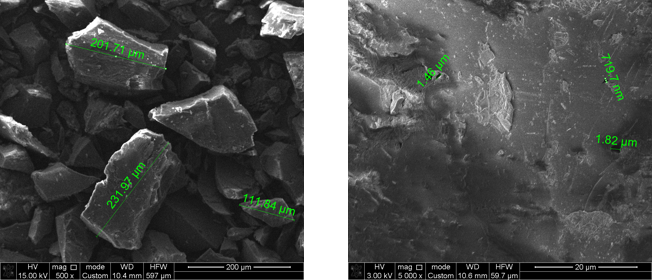
\includegraphics[width=0.8\textwidth]{assets/55}
	\caption*{}
\end{figure}

{\bfseries Figure 3 - SEM of the original coal «Shubarkol»}

\begin{figure}[H]
	\centering
	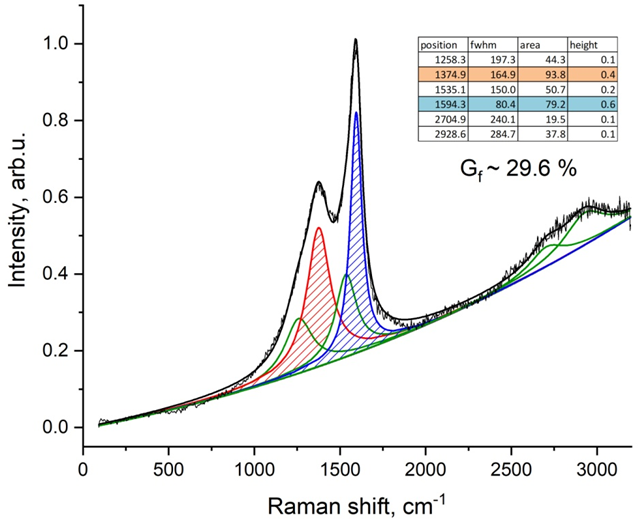
\includegraphics[width=0.8\textwidth]{assets/56}
	\caption*{}
\end{figure}

{\bfseries Figure 4 - Raman spectroscopy of the original coal «Shubarkol»}

After activation of Shubarkol coal, SEM images show that agglomerates of
different elements were removed. Pores are noticeable, with sizes
ranging from 155 nm to 33.08 µm. During the carbonization process,
mineral agglomerates opened, as shown in Fig. 5 by white spots. Peaks at
1194.4 are visible in the Raman spectrum; 1347.9; 1517.1; 1595.4;
2700.7; 2914.0 cm\textsuperscript{-1}. The degree of graphitization
after the activation process dropped to G\textsubscript{f}=24\%, this is
explained by the fact that peak D 1347.9 cm\textsuperscript{-1}
increased its intensity (Figure 6). I(D)/I(G)=0.9 I(G)/I(2D)=13.1.
Amorphous carbon with signs of graphitization - a narrow peak G, as well
as a weak manifestation of a second-order peak - 2D.

\begin{figure}[H]
	\centering
	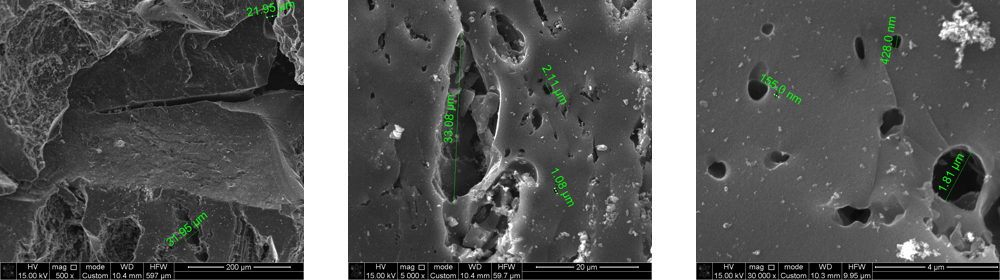
\includegraphics[width=0.8\textwidth]{assets/57}
	\caption*{}
\end{figure}

{\bfseries Figure 5 - SEM image of activated carbon «Shubarkol»}

\begin{figure}[H]
	\centering
	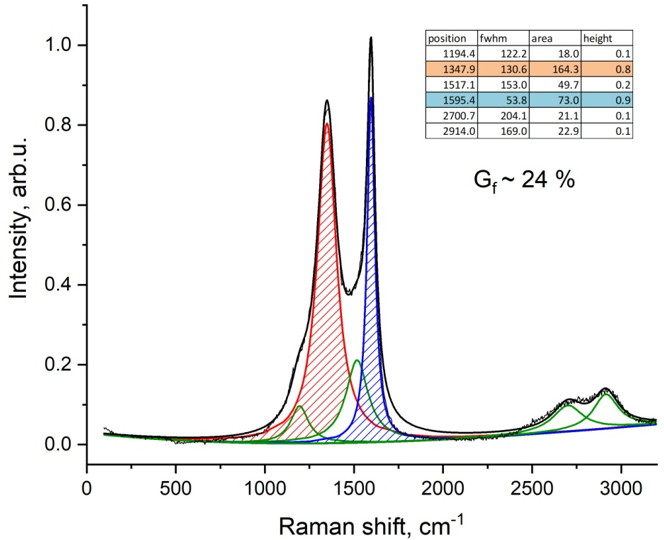
\includegraphics[width=0.8\textwidth]{assets/58}
	\caption*{}
\end{figure}

{\bfseries Figure 6 - Raman spectroscopy of activated carbon «Shubarkol»}

After the arc discharge, we see deformation of the pores in SEM images.
The pores have become smaller and range from 159.9 nm to 1.83 µm. The
formation of micro- and mesopores is assumed. White flake-like spots are
visible on the surface (Figure 7). As you can see in Fig. 8 there are
peaks at 1363.7(D); 1465; 1582.5(G); 2448.5; 2725.9(2D); 2959
cm\textsuperscript{-1} According to the Raman spectroscopy data, the
«Shubarkol» activated carbon after an arc discharge on the reactor walls
has a high degree of graphitization G\textsubscript{f} = 80.7\%.
Compared with activated carbon, peak D shows a weaker intensity, and
peak 2D shows a more prominent intensity. I(D)/I(G)=0.1, I(G)/I(2D)=2.9.
As a result, it can be said from the surface of the «Shubarkol»
activated carbon that after an arc discharge, graphene structures of
high quality and small thickness were formed on the walls of the
reactor.

\begin{figure}[H]
	\centering
	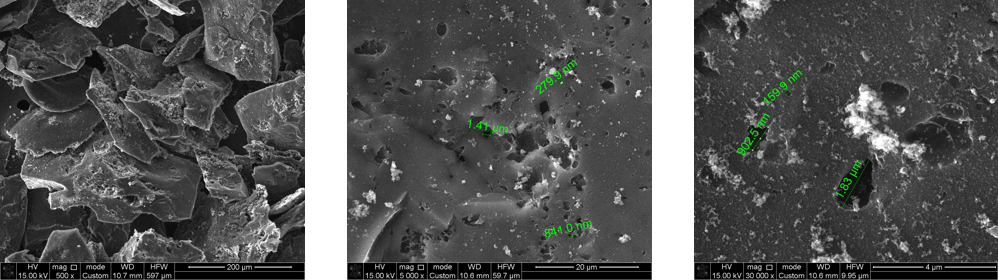
\includegraphics[width=0.8\textwidth]{assets/59}
	\caption*{}
\end{figure}

{\bfseries Figure 7 - SEM image of «Shubarkol» activated carbon after an
arc discharge on the walls of the reactor (100A, 75B)}

\begin{figure}[H]
	\centering
	\includegraphics[width=0.8\textwidth]{assets/60}
	\caption*{}
\end{figure}

{\bfseries Figure 8 - Raman spectroscopy of «Shubarkol» activated carbon
after an arc discharge on the walls of the reactor (100A, 75B)}

After an arc discharge, layers of graphene are visible on the surface of
the Shubarkol coal, according to the SEM image. Nanomaterials ranging in
size from 67.3 nm to 467.9 nm were formed. Pore
\hspace{0pt}\hspace{0pt}deformations are noticeable (Fig. 9). It is
assumed that layers of graphene have grown together on the surface of
the pores. In the Raman peaks at 1228.8 are noticeable; 1355.3(D);
1476.6; 1577.4(G); 2435.4; 2714.5(2D); 2935 cm\textsuperscript{-1}.
I(D)/I(G)=0.3 I(G)/I(2D)=2.8 From these data we can say that on the
surface of the Shubarkol activated carbon after an arc discharge on the
surface of the electrode there are graphene-like structures of varying
degrees of defects (Fig. 10).

\begin{figure}[H]
	\centering
	\includegraphics[width=0.8\textwidth]{assets/61}
	\caption*{}
\end{figure}

{\bfseries Figure 9 - SEM image of activated carbon «Shubarkol» after an
arc discharge on the surface of the electrode (100A, 75B)}

\begin{figure}[H]
	\centering
	\includegraphics[width=0.8\textwidth]{assets/62}
	\caption*{}
\end{figure}

{\bfseries Figure 10 - Raman spectroscopy of activated carbon «Shubarkol»
after an arc discharge on the surface of the electrode (100A, 75B)}

SEM images (Figure 11) of crushed Shubarkol coal used as an electrode
show nanodots of different diameters. The dots start from 29.5 nm to
8.95 µm. Peaks at 1249.1 are visible in the Raman distribution;
1357.4(D); 1472.6; 1584.6(G); 2459.1; 2725.3(D); 2937.4
cm\textsuperscript{-1}. I(D)/I(G)=0.4 I(G)/I(2D)=1.8. Graphene-like
structures of varying degrees of defects and thickness.

\begin{figure}[H]
	\centering
	\includegraphics[width=0.8\textwidth]{assets/63}
	\caption*{}
\end{figure}

{\bfseries Figure 11 - SEM image of «Shubarkol» activated carbon after an
arc discharge (100A, 75B)}

\begin{figure}[H]
	\centering
	\includegraphics[width=0.8\textwidth]{assets/64}
	\caption*{}
\end{figure}

{\bfseries Figure 12 - Raman spectroscopy of «Shubarkol» activated carbon
after an arc discharge}

{\bfseries (100A, 75B)}

It is known that the 2D band of Raman spectra is more sensitive to the
overlay of graphene sheets. From the Raman scattering data (Raman
effect), the intensities of the D, G and 2D peaks were calculated. It is
immediately noticeable that after activation the G peak increased its
intensity from 0.6 to 0.9. After the arc discharge, peak D loses its
intensity, and peak 2D increased its intensity from 0.1 to 0.51. The
intensity ratios I2D/IG for one-, two-, three- and multilayer
(\textgreater{} 4) in these materials were shown to vary from 0.11 to
0.54. And the ratio of IG/I2D peaks after arc treatment is from 1.84 to
2.94, which confirms the formation of two to three layer graphene (for
single-layer graphene the ratio is 0.6-1). The Raman spectrum of the
material with the lowest degree of crystallization contains a strong
D-band and a broad and weak G-band, and their high

{\bfseries Table 1 - Ratio of D G and 2D peaks in materials obtained from
Shubarkol coal}

intensity ratio (ID/IG) confirms the strong disorder of the structure.
Based on the intensity ratio of the ID/IG bands after an arc discharge,
which ranges from 0.12 to 0.38, it can be argued that there are a small
number of material defects. Based on these data, we can say that we have
obtained modern carbon materials of very good quality.

\begin{longtable}[]{@{}
  >{\raggedright\arraybackslash}p{(\columnwidth - 20\tabcolsep) * \real{0.1176}}
  >{\raggedright\arraybackslash}p{(\columnwidth - 20\tabcolsep) * \real{0.0884}}
  >{\raggedright\arraybackslash}p{(\columnwidth - 20\tabcolsep) * \real{0.0883}}
  >{\raggedright\arraybackslash}p{(\columnwidth - 20\tabcolsep) * \real{0.0884}}
  >{\raggedright\arraybackslash}p{(\columnwidth - 20\tabcolsep) * \real{0.0883}}
  >{\raggedright\arraybackslash}p{(\columnwidth - 20\tabcolsep) * \real{0.0884}}
  >{\raggedright\arraybackslash}p{(\columnwidth - 20\tabcolsep) * \real{0.0883}}
  >{\raggedright\arraybackslash}p{(\columnwidth - 20\tabcolsep) * \real{0.0884}}
  >{\raggedright\arraybackslash}p{(\columnwidth - 20\tabcolsep) * \real{0.0883}}
  >{\raggedright\arraybackslash}p{(\columnwidth - 20\tabcolsep) * \real{0.0884}}
  >{\raggedright\arraybackslash}p{(\columnwidth - 20\tabcolsep) * \real{0.0876}}@{}}
\toprule\noalign{}
\multirow{2}{=}{\begin{minipage}[b]{\linewidth}\raggedright
Elements
\end{minipage}} &
\multicolumn{2}{>{\raggedright\arraybackslash}p{(\columnwidth - 20\tabcolsep) * \real{0.1766} + 2\tabcolsep}}{%
\begin{minipage}[b]{\linewidth}\raggedright
Source coal «Shubarkol»
\end{minipage}} &
\multicolumn{2}{>{\raggedright\arraybackslash}p{(\columnwidth - 20\tabcolsep) * \real{0.1766} + 2\tabcolsep}}{%
\begin{minipage}[b]{\linewidth}\raggedright
Activated carbon «Shubarkol»
\end{minipage}} &
\multicolumn{2}{>{\raggedright\arraybackslash}p{(\columnwidth - 20\tabcolsep) * \real{0.1766} + 2\tabcolsep}}{%
\begin{minipage}[b]{\linewidth}\raggedright
Activated carbon «Shubarkol»

After arcing

(on the walls of the reactor)
\end{minipage}} &
\multicolumn{2}{>{\raggedright\arraybackslash}p{(\columnwidth - 20\tabcolsep) * \real{0.1766} + 2\tabcolsep}}{%
\begin{minipage}[b]{\linewidth}\raggedright
Activated carbon «Shubarkol»

after arc discharge

(on the surface of the electrode)
\end{minipage}} &
\multicolumn{2}{>{\raggedright\arraybackslash}p{(\columnwidth - 20\tabcolsep) * \real{0.1760} + 2\tabcolsep}@{}}{%
\begin{minipage}[b]{\linewidth}\raggedright
Activated carbon «Shubarkol»

after an arc discharge (crushed electrode)
\end{minipage}} \\
& \begin{minipage}[b]{\linewidth}\raggedright
Wt\%
\end{minipage} & \begin{minipage}[b]{\linewidth}\raggedright
At\%
\end{minipage} & \begin{minipage}[b]{\linewidth}\raggedright
Wt\%
\end{minipage} & \begin{minipage}[b]{\linewidth}\raggedright
At\%
\end{minipage} & \begin{minipage}[b]{\linewidth}\raggedright
Wt\%
\end{minipage} & \begin{minipage}[b]{\linewidth}\raggedright
At\%
\end{minipage} & \begin{minipage}[b]{\linewidth}\raggedright
Wt\%
\end{minipage} & \begin{minipage}[b]{\linewidth}\raggedright
At\%
\end{minipage} & \begin{minipage}[b]{\linewidth}\raggedright
Wt\%
\end{minipage} & \begin{minipage}[b]{\linewidth}\raggedright
At\%
\end{minipage} \\
\midrule\noalign{}
\endhead
\bottomrule\noalign{}
\endlastfoot
C & 77,15 & 82 & 90,35 & 92,92 & 87,21 & 90,40 & 71,70 & 85,89 & 83,49 &
90,83 \\
O & 22,24 & 17,74 & 8,57 & 6,62 & 11,75 & 9,15 & 6,51 & 5,86 & 7,84 &
6,40 \\
Al & 0,4 & 0,19 & 0,35 & 0,16 & 0,36 & 0,16 & 2,04 & 1,09 & 0,6 &
0,29 \\
Si & 0,07 & 0,03 & 0,11 & 0,05 & 0,19 & 0,08 & 7,68 & 3,94 & 0,44 &
0,21 \\
Ca & - & - & 0,29 & 0,09 & 0,25 & 0,08 & 0,25 & 0,09 & 1,41 & 0,46 \\
Mg & - & - & 0,11 & 0,05 & - & - & 0,18 & 0,11 & 0,49 & 0,26 \\
Na & - & - & 0,12 & 0,06 & 0,25 & 0,13 & - & - & 0,40 & 0,22 \\
S & - & - & 0,11 & 0,04 & - & - & 0,20 & 0,09 & 0,46 & 0,19 \\
Fe & 0,15 & 0,03 & - & - & - & - & 11,42 & 2,94 & 4,87 & 1,14 \\
\end{longtable}

{\bfseries Table 2 - Elemental composition of the initial, activated and
after arc discharge of Shubarkol coal}

\begin{longtable}[]{@{}
  >{\raggedright\arraybackslash}p{(\columnwidth - 14\tabcolsep) * \real{0.2838}}
  >{\raggedright\arraybackslash}p{(\columnwidth - 14\tabcolsep) * \real{0.0680}}
  >{\raggedright\arraybackslash}p{(\columnwidth - 14\tabcolsep) * \real{0.0680}}
  >{\raggedright\arraybackslash}p{(\columnwidth - 14\tabcolsep) * \real{0.0802}}
  >{\raggedright\arraybackslash}p{(\columnwidth - 14\tabcolsep) * \real{0.1186}}
  >{\raggedright\arraybackslash}p{(\columnwidth - 14\tabcolsep) * \real{0.1186}}
  >{\raggedright\arraybackslash}p{(\columnwidth - 14\tabcolsep) * \real{0.1314}}
  >{\raggedright\arraybackslash}p{(\columnwidth - 14\tabcolsep) * \real{0.1314}}@{}}
\toprule\noalign{}
\begin{minipage}[b]{\linewidth}\raggedright
Name
\end{minipage} & \begin{minipage}[b]{\linewidth}\raggedright
I(D)
\end{minipage} & \begin{minipage}[b]{\linewidth}\raggedright
I(G)
\end{minipage} & \begin{minipage}[b]{\linewidth}\raggedright
I(2D)
\end{minipage} & \begin{minipage}[b]{\linewidth}\raggedright
I(D)/I(G)
\end{minipage} & \begin{minipage}[b]{\linewidth}\raggedright
I(G)/I(D)
\end{minipage} & \begin{minipage}[b]{\linewidth}\raggedright
I(G)/I(2D)
\end{minipage} & \begin{minipage}[b]{\linewidth}\raggedright
I(2D)/I(G)
\end{minipage} \\
\midrule\noalign{}
\endhead
\bottomrule\noalign{}
\endlastfoot
Source coal "Shubarkol" & 0,4 & 0,6 & 0,1 & 0,67 & 1,5 & 6 & 0,17 \\
Activated carbon "Shubarkol" & 0,8 & 0,9 & 0,1 & 0,89 & 1,12 & 9 &
0,11 \\
After an arc discharge (on the reactor walls) & 0,12 & 1 & 0,34 & 0,12 &
8,33 & 2,94 & 0,34 \\
After an arc discharge (on the surface of the electrode) & 0,25 & 0,93 &
0,33 & 0,27 & 3,72 & 2,8 & 0,35 \\
After an arc discharge (crushed electrode) & 0,36 & 0,94 & 0,51 & 0,38 &
2,61 & 1,84 & 0,54 \\
\end{longtable}

Based on the elemental composition, we can say that the original
Shubarkol coal contains 77.15\% carbon; this figure increased to 90.35\%
after the activation process. In addition, the oxygen concentration
decreased from 22.24\% to 8.57\% and minerals such as calcium and
magnesium were discovered and accounted for Ca-0.29\% and Mg-0.11\% of
the total mass. Also noticeable is the low concentration of sodium and
sulfur after the activation process (Na-0.12\%, S-0.11\%). Some
elements, such as aluminum and silicon, did not change much after
activation (Al-0.35\%, Si-0.11\%), and iron completely disappeared from
the surface of Shubarkol coal during activation. Analysis of the
elemental composition shows that activated carbon after electric arc
contains 71.70-87.21\% C 6.51-11.75\% O. In addition to carbon and
oxygen, CNM on the reactor walls contains small amounts of aluminum,
silicon, calcium and sodium (Al-0.36\% , Si-0.19\%, Ca-0.25\%,
Na-0.25\%). On the surface of the electrode there are elements such as
aluminum, silicon, calcium, magnesium, sulfur and iron (Al-2.04\%,
Si-7.68\%, Ca-0.25\%, Mg-0.18\%, S-0 .2\%, Fe-11.42\%). The crushed
electrode has different concentrations of aluminum, silicon, calcium,
magnesium, sodium, sulfur and iron (Al-0.6\%, Si-0.44\%, Ca-1.41\%,
Mg-0.49\%, Na- 0.4\%, S-0.46\%, Fe-4.87\%. The highest indicator of
aluminum, silicon, and iron was shown by activated carbon after an arc
discharge on the walls of the reactor, and for magnesium, calcium,
sodium and sulfur, the highest concentration was activated carbon after
an arc discharge, crushed electrode.

As can be seen in Fig. 13 The original Shubarkol coal does not exhibit
semiconductor properties, the dielectric constant over the entire
temperature range under study is very low and this material is not of
electrical interest.

\begin{figure}[H]
	\centering
	\includegraphics[width=0.8\textwidth]{assets/65}
	\caption*{}
\end{figure}

\begin{figure}[H]
	\centering
	\includegraphics[width=0.8\textwidth]{assets/66}
	\caption*{}
\end{figure}

А Б

{\bfseries Figure 13 - Dependence of dielectric constant (A) and electrical
resistance (B) on temperature at a frequency of 1 kHz}

Activated carbon «Shubarkol» shows that the dielectric constant of this
material has mainly average values. The maximum value of ε is achieved
at 393 K -- 2.62·10\textsuperscript{6} (1 kHz),
7.23·10\textsuperscript{5} (5 kHz) and 3.73·10\textsuperscript{5} (10
kHz). A study of the temperature dependence of electrical resistance
shows that activated carbon exhibits variable conductivity in the range
of 293-333 K, semiconductor conductivity at 333-393 K, metallic
conductivity at 393-453 K, and variable conductivity at 453-483 K.

Activated carbon "Shubarkol" after an arc discharge obtained on the
walls of the reactor at 293 K exhibits a high value of ε
(6.77·10\textsuperscript{6}) - 1 kHz, 3.72·10\textsuperscript{5} - 5 kHz
and 1.08·10\textsuperscript{5} - 10 kHz and reaches colossal values
\hspace{0pt}\hspace{0pt}at 443 - 483 K 7.20·10\textsuperscript{8} and
more (1 kHz), 2.50·10\textsuperscript{8} (5 kHz and 483 K) and
8.41·10\textsuperscript{7} (10 kHz and 483 K). A study of the
temperature dependence of the electrical resistance of material III
shows variable conductivity in the range of 293-333 K, semiconductor
conductivity at 333-423 K, and semiconductor conductivity again at
433-483 K.

Activated carbon «Shubarkol» after an arc discharge obtained on the
surface of the electrode already at lower temperatures of 293 and 343
shows gigantic values \hspace{0pt}\hspace{0pt}of dielectric constant
6.16·10\textsuperscript{7} (1 kHz), 2.90·10\textsuperscript{6} (5 kHz)
and 2.45·10\textsuperscript{6} (10 kHz) at 313 K and starting from 403 K
at 1 kHz is also ε greater than 1.44·10\textsuperscript{8} and colossal
values \hspace{0pt}\hspace{0pt}of ε are maintained (albeit with a
decrease) at frequencies of 5 and 10 kHz. Activated carbon «Shubarkol»
after an arc discharge (on the surface of the electrode) in the range of
293-463 K exhibits semiconductor conductivity, and at 463-483 K -- mixed
conductivity.

According to the temperature dependence of the dielectric constant of
Activated carbon «Shubarkol» after an arc discharge, the crushed
electrode shows that already at 293 K it shows a gigantic value at a
frequency of 1 kHz and at frequencies of 5 and 10 kHz high values
\hspace{0pt}\hspace{0pt}of dielectric constant:
1.56·10\textsuperscript{7} (1 kHz), 9.83·10\textsuperscript{5} (5 kHz)
and 2.78·10\textsuperscript{5} (10 kHz). The colossal value of ε is
achieved at 463 K and 1 kHz (8.63·10\textsuperscript{8}). The
temperature dependence of electrical resistance in the range of 293-333
K exhibits metallic conductivity, at 333-433 K - semiconductor
conductivity, and at 433-483 K - variable conductivity.

As shown in Table 3, dielectric constant is inversely proportional to
frequency. Materials after an arc discharge increased their dielectric
constant. The most optimal indicator for activated carbon after an arc
discharge is obtained on the walls of the reactor. For comparison, we
gave the example of graphite and the resulting materials have a similar
dielectric constant. The band gap of the resulting materials can be
classified as narrow-gap semiconductors. Activated carbons after arc
processing are of interest for semiconductor and microcapacitor
technology.

{\bfseries Table 3 - Dependence of dielectric constant (ε) on temperature
at different frequencies}

\begin{longtable}[]{@{}
  >{\raggedright\arraybackslash}p{(\columnwidth - 12\tabcolsep) * \real{0.1450}}
  >{\raggedright\arraybackslash}p{(\columnwidth - 12\tabcolsep) * \real{0.1595}}
  >{\raggedright\arraybackslash}p{(\columnwidth - 12\tabcolsep) * \real{0.1481}}
  >{\raggedright\arraybackslash}p{(\columnwidth - 12\tabcolsep) * \real{0.1448}}
  >{\raggedright\arraybackslash}p{(\columnwidth - 12\tabcolsep) * \real{0.1418}}
  >{\raggedright\arraybackslash}p{(\columnwidth - 12\tabcolsep) * \real{0.1304}}
  >{\raggedright\arraybackslash}p{(\columnwidth - 12\tabcolsep) * \real{0.1304}}@{}}
\toprule\noalign{}
\multirow{3}{=}{\begin{minipage}[b]{\linewidth}\raggedright
Name of material
\end{minipage}} &
\multicolumn{6}{>{\raggedright\arraybackslash}p{(\columnwidth - 12\tabcolsep) * \real{0.8550} + 10\tabcolsep}@{}}{%
\begin{minipage}[b]{\linewidth}\raggedright
The dielectric constant (ε)
\end{minipage}} \\
&
\multicolumn{2}{>{\raggedright\arraybackslash}p{(\columnwidth - 12\tabcolsep) * \real{0.3076} + 2\tabcolsep}}{%
\begin{minipage}[b]{\linewidth}\raggedright
at 1 kHz
\end{minipage}} &
\multicolumn{2}{>{\raggedright\arraybackslash}p{(\columnwidth - 12\tabcolsep) * \real{0.2865} + 2\tabcolsep}}{%
\begin{minipage}[b]{\linewidth}\raggedright
at 5 kHz
\end{minipage}} &
\multicolumn{2}{>{\raggedright\arraybackslash}p{(\columnwidth - 12\tabcolsep) * \real{0.2609} + 2\tabcolsep}@{}}{%
\begin{minipage}[b]{\linewidth}\raggedright
at 10 kHz
\end{minipage}} \\
& \begin{minipage}[b]{\linewidth}\raggedright
293
\end{minipage} & \begin{minipage}[b]{\linewidth}\raggedright
483
\end{minipage} & \begin{minipage}[b]{\linewidth}\raggedright
293
\end{minipage} & \begin{minipage}[b]{\linewidth}\raggedright
483
\end{minipage} & \begin{minipage}[b]{\linewidth}\raggedright
293
\end{minipage} & \begin{minipage}[b]{\linewidth}\raggedright
483
\end{minipage} \\
\midrule\noalign{}
\endhead
\bottomrule\noalign{}
\endlastfoot
BaTiO\textsubscript{3} & 1296 & 2159 & 1220 & 2102 & 561 & 2100 \\
Graphite & 6,07*\(10^{7}\) & 7,19*\(10^{8}\)\textless{} &
4,04*\(10^{6}\) & 2,56*\(10^{8}\) & 1,15*\(10^{6}\) & 8,70*\(10^{7}\) \\
On the walls of the reactor & 6770953 & 719702040˂ & 371895 & 249796682
& 107561 & 84141207 \\
On the surface of the electrode & 61630141 & 143940408˂ & 2898125 &
69699521 & 2453921 & 22287956 \\
Crushed electrode & 15614812 & 45948829 & 982576 & 2055749 & 277845 &
601308 \\
\end{longtable}

Since the nanomaterial obtained on the walls of the reactor showed the
best results in terms of physicochemical and electrophysical properties,
the material was tested for hydrogen storage. The specific surface area
according to Langmuir theory is 112.27 m\textsuperscript{2}/g, and
according to BET - 104,08 m\textsuperscript{2}/g. For the case of 77 K,
it is also possible to determine the specific surface area and pore
distribution using DFT methods for carbon materials: total area in pores
(\textgreater= 2,91 Å) - 1 099,971 m²/g (H\textsubscript{2}). Based on
these data, the percentage of absorbed hydrogen on the adsorbent was
calculated. Nonmaterial on the walls of the reactor absorbed 0.314\%
(35.1516 cm\textsuperscript{3}/g) of the total mass.

{\bfseries Conclusions.} When conducting an experiment using an electric
arc discharge at a high current of 100 amperes, graphene and materials
containing graphene are formed both on the walls of the reactor and in
the electrode itself. The optimal degree of graphitization of 80.7\% is
achieved when graphene-containing material is formed on the walls of the
reactor after an arc discharge. The method of producing graphene through
electric arc discharge is promising and provides high purity and a
minimum number of defects in the product. It has many advantages such as
low cost, high efficiency and catalyst-free synthesis. This method is
easily scalable from laboratory conditions to industrial processes.

The use of graphene in various industries such as batteries, capacitors
and composite materials will help solve environmental problems. Graphene
has unique physical properties that make it attractive to researchers
and engineers. Some experts believe that graphene could replace silicon
transistors in the future due to its cost-effectiveness and speed.

The environmental aspect of the method lies in the ability to use coal
and carbon products to produce graphene, which will avoid the use of
chemical compounds and reagents. Thanks to this, environmentally
friendly technology with high added value of products is created.

Thus, the study made it possible to obtain important data on the
dynamics of the process of hydrogen adsorption on a porous carbon
material, its speed and efficiency. These results can be useful in the
development and optimization of hydrogen adsorption processes for
various industrial and scientific applications.

\emph{{\bfseries Financing:} The research was carried out with the
financial support of the Science Committee of the Ministry of Science
and Higher Education of the Republic of Kazakhstan (Grant No.
AR19577512. Development of scientific and technical foundations for the
production of microporous carbon nanomaterials for the separation and
storage of hydrogen).}

{\bfseries References}

1.Jia X., Wei F. Advances in production and applications of carbon
nanotubes //Single-Walled Carbon Nanotubes: Preparation, Properties and
Applications.- 2019.- P. 299-333.

DOI10.1007/s41061-017-0102-2

2.Shmalko V.M.. Keush L. G. Zelenskiy O.I. Nanomaterialy iz uglya i
produktov ego piroliza // Dnepr. Lira. - 2018. -142 s. ISBN
978-966-981-030-4 (In Russian)

3.Janas D., ``Perfectly imperfect: a review of chemical tools for
exciton engineering in single-walled carbon nanotubes,'' Materials
Horizons. - 2020. - V.7. - No.11. - P. 2860 - 2881.

DOI 10.1039/D0MH00845A

4.Kukovecz Á., Kozma G., and Kónya Z. ``Multi-Walled Carbon Nanotubes,''
in Springer handbook of nanomaterials, Springer, Berlin, Heidelberg. -
2013.- P. 147-188.

DOI 10.1007/978-3-642-20595-8\_5

5.Mubarak N., Abdullah E., Jayakumar N., Sahu J. An overview on methods
for the production of carbon nanotubes// Journal of Industrial and
Engineering Chemistry. -2014. - V. 20(4).- P. 1186- 1197. DOI 1197.DOI
10.1016/j.jiec.2013.09.001

6.Osmani R.M, Kulkarni A.S, Aloorkar N.H, Bhosale R.R, Ghodake P.P,
Harkare B.R Carbon nanotubes: an impending carter in therapeutics // Int
J Pharmaceut Clin Res. - 2014.- V. 6(1) - P.84-96.

7.Hong, S., Myung, S. A flexible approach to mobility // Nature
Nanotech~2. - 2007. - P. 207-208. DOI 10.1038/nnano.2007.89

8.Diachkov P.N. Elektronnyye svoystva i primeneniye nanotrubok. --
Izd-vo: Binom. Laboratoriya znaniy. - 2014. -- 488 s. ISBN:
978-5-9963-0154-6 (In Russian)

9.Cotul U., Parmak E.D., Kaykilarli C., Saray O., Uzunsoy D., Colak O.
Development of High Purity // Few-Layer Graphene Synthesis by Electric
Arc Discharge Technique. - 2018. - V. 134. --P. 289-291. DOI
10.12693/aphyspola.134.289

10.Nan Li, Zhiyong Wang, Zujin Shi. Synthesis of Graphenes with
Arc-Discharge Method // Physics and Applications of Graphene --
Experiments.- 2011.-P.23-35.DOI 10.5772/14961

11.Yu X., Tang Z., Sun D. et al. Recent advances and remaining
challenges of nanostructured materials for hydrogen storage
applications// Prog. Mater. Sci. - 2017. - V. 88. - P. 1- 48.

DOI 10.1016/j.pmatsci.2017.03.001

12.Stoller M.D., Park S., Zhu Y. et al. // Graphene-Based
Ultracapacitors //Nano Lett. - 2008. - Vol. 8(10) - P. 3498-3502. DOI
10.1021/nl802558y.

13.Khan, U., O\textquotesingle Neill, A., Lotya, M., De, S. and Coleman,
J.N. High-Concentration Solvent Exfoliation of Graphene //Small. -2010.-
V.6. - P.864-871. DOI10.1002/smll.200902066

14. Gao W.. The Chemistry of Graphene Oxide, Eds. W. Gao, Springer,
Switzerland. -2015.-P. 61-95. DOI 10.1007/978-3-319-15500-5\_3~

15.Li N. et al. Large scale synthesis of N-doped multi-layered graphene
sheets by simple arc-discharge method // Carbon.- 2010.- Vol. 48 (1)-
P.255-259. DOI 10.1016/j.carbon.2009.09.013.

16.Çotul U. et al. Development of high purity, few-layer graphene
synthesis by electric arc discharge technique // Acta Physica Polonica
A.- 2018.-Vol.134 (1)- P.289-291.

DOI 10.12693/APhysPolA.134.289.

\emph{{\bfseries Information about the authors}}

Kazankapova M.K. -PhD in Philosophy, assoc. professor, member
correspondent of the KazNANS, Leading Researcher, Head of Laboratory of
LLP "Institute of Coal Chemistry and Technology", Astana, Kazakhstan,
e-mail: maira\_1986@mail.ru;

Yermagambet B.T.{\bfseries -}Doctor of Chemical Science, Professor,
Academician of the KazNANS, Project Manager, Chief Researcher, Director
of LLP "Institute of Coal Chemistry and Technology", Astana, Kazakhstan,
e-mail: bake.yer@mail.ru;

Mendaliyev G.K.{\bfseries -}master student Eurasian National University of
L.N. Gumilyov{\bfseries ,} Astana, Kazakhstan, e-mail: ganimen@mail.ru;

Samatkyzy A.- laboratory assistant "Institute of Coal Chemistry and
Technology" LLP, Astana, Kazakhstan, e-mail: akshekina11@mail.ru;

Malgazhdarova A.B.-master student Eurasian National University of L.N.
Gumilyov{\bfseries ,} Astana, Kazakhstan, e-mail: malgazhdarova.ab@mail.ru

\emph{{\bfseries Сведения об авторах}}

Казанкапова М.К. -PhD философских наук, асс. профессор, чл.-корр.
КазНАЕН, ведущий научный сотрудник, заведующий лабораторией ТОО
«Институт химии и технологии угля», Астана, Казахстан, e-mail:
maira\_1986@mail.ru;

Ермагамбет Б.Т.-доктор химических наук, профессор, академик КазНАЕН,
руководитель проекта, главный научный сотрудник, директор ТОО «Институт
химии и технологии угля», Астана, Казахстан, e-mail: bake.yer@mail.ru;

Мендалиев Г.К.- магистрант Евразийского национального университета им.
Л.Н. Гумилева, Астана, Казахстан, e-mail: ganimen@mail.ru;

Саматкызы А.{\bfseries -}лаборант ТОО «Институт химии угля и технологии»,
Астана, Казахстан, e-mail: akshekina11@mail.ru;

Малгаждарова А.Б.- магистрант Евразийского национального университета
им. Л.Н. Гумилева, Астана, Казахстан, e-mail: malgazhdarova.ab@mail.ru\newpage
{\bfseries МРНТИ 61.53.15}

{\bfseries ИССЛЕДОВАНИЕ ФИЗИКО-ХИМИЧЕСКИХ ХАРАКТЕРИСТИК УГЛЯ И ПРОДУКТОВ
ЕГО ПИРОЛИЗА}

{\bfseries \textsuperscript{1,2}Н.У. Нургалиев, \textsuperscript{1}Ж.Б.
Искакова, \textsuperscript{3}А. Колпек, \textsuperscript{1}Е.К.
Айбульдинов,}

{\bfseries \textsuperscript{3}А.С. Сабитов , \textsuperscript{3}Э.Е.
Копишев, \textsuperscript{1,4}Р.М. Салихов, \textsuperscript{1,4}М.С.
Петров, \textsuperscript{1}Г.Ж. Алжанова,}

{\bfseries \textsuperscript{1,5}Г.Г. Абдиюсупов, \textsuperscript{1,6}М.Т.
Өмірзақ}

\textsuperscript{1}Научно-исследовательский институт Новых химических
технологий, Евразийский национальный университет им. Л.Н. Гумилева,
Астана, Казахстан,

\textsuperscript{2}Казахский университет технологии и бизнеса им. К.
Кулажанова, Астана, Казахстан,

\textsuperscript{3}Евразийский национальный университет им. Л.Н.
Гумилева, Астана, Казахстан,

\textsuperscript{4} ООО «ТТУ ЛТД», Санкт-Петербург, Россия,

\textsuperscript{5}CCS Services -- Central Asia, Алматы, Казахстан,

\textsuperscript{6}Sauda Exports\&Import, Алматы, Казахстан

Корреспондент-автор: nurgaliev\_nao@mail.ru , zhanariskakova@mail.ru,
elaman\_@mail.ru

В статье проведен низкотемпературный пиролиз угля месторождения
«Сарыадыр» с определением физико-химических свойств угля и продуктов его
термической деструкции. Выполнены элементный анализ угля и анализ
минеральной части угля. Проведены 6 параллельных опытов процесса
низкотемпературного пиролиза угля, в результате которых определены
выходы таких продуктов, как полукокс, смола, горючий газ, а также
определены их основные характеристики (компонентный состав, теплотворная
способность и др.). При этом сходимость результатов (от 6 опытов) вполне
удовлетворительна. Проведен тепловой баланс пиролиза угля с учетом
усредненных выходов продуктов.

{\bfseries Ключевые слова:} уголь, пиролиз, полукокс, смола, горючий газ,
тепловой баланс

{\bfseries КӨМІРДІҢ ЖӘНЕ ОНЫҢ ПИРОЛИЗ ӨНІМДЕРІНІҢ ФИЗИКА-ХИМИЯЛЫҚ
СИПАТТАМАЛАРЫН ЗЕРТТЕУ}

{\bfseries \textsuperscript{1,2}Н.У. Нургалиев, \textsuperscript{1}Ж.Б.
Искакова, \textsuperscript{3}А. Колпек, \textsuperscript{1}Е.К.
Айбульдинов,}

{\bfseries \textsuperscript{3}А.С. Сабитов, \textsuperscript{3}Э.Е.
Копишев, \textsuperscript{1,4}Р.М. Салихов, \textsuperscript{1,4}М.С.
Петров, \textsuperscript{1}Г.Ж. Алжанова,}

{\bfseries \textsuperscript{1,5}Г.Г. Абдиюсупов, \textsuperscript{1,6}М.Т.
Өмірзақ}

\textsuperscript{1}Жаңа химиялық технологиялар ғылыми-зерттеу институты,
Л.Н. Гумилев атындағы Еуразия ұлттық университеті, Астана,Қазақстан,

\textsuperscript{2}Қ.Құлажанов атындағы технология және бизнес
университеті, Астана, Қазақстан,

\textsuperscript{3}Л.Н. Гумилев атындағы Еуразия ұлттық университеті,
Астана, Қазақстан,

\textsuperscript{4} ООО «ТТУ ЛТД», Санкт-Петербург, Россия,

\textsuperscript{5}CCS Services -- Central Asia, Алматы, Қазақстан,

\textsuperscript{6}Sauda Exports\&Import, Алматы, Қазақстан,

e-mail: nurgaliev\_nao@mail.ru , zhanariskakova@mail.ru,
elaman\_@mail.ru

Мақалада көмірдің физика-химиялық қасиеттерін және оның термиялық
деструкция өнімдерін анықтай отырып, "Сарыадыр" кен орнының төмен
температуралы көмір пиролизінің жүргізілуі келтірілген. Көмірдің
элементтік талдауы және көмірдің минералды бөлігінің талдауы берілген.
Көмірдің төмен температуралы пиролиз процесінің 6 параллель тәжірибесі
жүргізілді, нәтижесінде жартылай кокс, шайыр, жанғыш газ сияқты
өнімдердің шығымы анықталды, сондай-ақ олардың негізгі сипаттамалары
(компоненттік құрамы, калориялық құндылығы және т.б.) анықталды. Сонымен
қатар, нәтижелердің тоғысуы (6 тәжірибеден) айтарлықтай қанағаттанарлық.
Өнімдердің орташа шығымдылығын ескере отырып, көмір пиролизінің жылу
балансы жүргізілді.

{\bfseries Түйін сөздер:} көмір, пиролиз, жартылай кокс, шайыр, жанғыш газ,
жылу балансы

{\bfseries STUDY OF PHYSICO-CHEMICAL CHARACTERISTICS OF COAL AND ITS
PYROLYSIS PRODUCTS}

{\bfseries \textsuperscript{1,2}N.U. Nurgaliyev, \textsuperscript{1}Zh.B.
Iskakova, \textsuperscript{3}А. Kolpek, \textsuperscript{1}Ye.K.
Aibuldinov,}

{\bfseries A\textsuperscript{3}.S. Sabitov, \textsuperscript{3}E.Ye.
Kopishev, \textsuperscript{1,4}R.M. Salikhov, \textsuperscript{1,4}M.S.
Petrov, \textsuperscript{1}G.Zh. Alzhanova,\\
\textsuperscript{1,5}G.G. Abdiyussupov, \textsuperscript{1,6}М.Т.
Omirzak}

\textsuperscript{1} Research Institute of New Chemical Technologies,
L.N. Gumilyov Eurasian National University, Astana, Kazakhstan,

\textsuperscript{2} Kazakh University of Technology and Business named
after K. Kulazhanov, Astana, Kazakhstan,

\textsuperscript{3}L.N. Gumilyov Eurasian National University, Astana,
Kazakhstan,

\textsuperscript{4} TTU LTD, St. Petersburg, Russia,

\textsuperscript{5}CCS Services -- Central Asia, Almaty, Kazakhstan,

\textsuperscript{6}Sauda Exports\&Import, Almaty, Kazakhstan,

e-mail: nurgaliev\_nao@mail.ru , zhanariskakova@mail.ru,
elaman\_@mail.ru

In the article low-temperature pyrolysis of coal of ``Saryadyr'' deposit
with determination of physical and chemical properties of coal and
products of its thermal destruction is carried out. Elemental analysis
of coal and analysis of mineral part of coal were carried out. 6
parallel experiments of the process of low-temperature pyrolysis of coal
were carried out, as a result of which the yields of such products as
semi-coke, tar, combustible gas were determined, as well as their main
characteristics (component composition, calorific value, etc.) were
determined. The convergence of the results (from 6 experiments) is quite
satisfactory. The thermal balance of coal pyrolysis was carried out
taking into account the average yields of products.

{\bfseries Keywords:} coal, pyrolysis, semi-coke, tar, combustible gas,
heat balance.

{\bfseries Введение.}Топливно-энергетические ресурсы являются основой
экономики Казахстана, среди которых особо выделяются нефть, уголь, газ.
Казахстан входит в топ-10 стран по доказанным запасам угля (около 2,4\%
мировых запасов), где 2/3 приходится на бурый уголь, 1/3 -- на каменный
уголь.

Будучи ценным горючим ископаемым, уголь остается мировым лидером по
использованию в топливно-энергетическом комплексе и применяется для
получения металлургического кокса, смолы, углеродных материалов,
гуминовых кислот, сырья для химической промышленности (бензол, толуол,
ксилол и др.) {[}1-3{]}. Из угля извлекают высокоценные жидкие и
газообразные топлива с полным использованием структуры и реакционной
способности угля {[}4,5{]}.~

Для эффективного использования угля важно понимать структуру угля.
Органическую структуру угля принято считать сложным полимером с высокой
степенью сшивки, включающим ароматические и алифатические компоненты
{[}6{]}, {[}7{]}. Имеются существенные различия в органическом строении
углей разной степени метаморфизма {[}8{]}, а также очевидные различия в
промышленном применении.~Тщательное знание структуры угля различной
степени метаморфизма необходимо для эффективного использования угольных
ресурсов.

В настоящее время среди существующих методов термопереработки угля
пиролиз является наиболее перспективным и исследуемым термическим
направлением переработки таких отходов, как низкосортные угли,
нефтешламы и др. {[}9{]}. Пиролиз представляет собой общую стадию многих
процессов, таких как сжигание, сжижение, карбонизация, газификация,
которые обычно работают в тесных системах в инертной, восстановительной
или окислительной атмосфере при различных давлениях и времени пребывания
{[}10{]}. Среди ценных продуктов (получаемых из угля) каменноугольная
смола является основным продуктом пиролиза и может использоваться в
качестве важного сырья для получения олефинов~{[}11,12{]}, ароматических
соединений с добавленной стоимостью {[}13{]}, и материалов на основе
каменноугольной смолы {[}11{]}.~

Целью данной работы является исследование процесса низкотемпературного
пиролиза (полукоксование) угля месторождения «Сарыадыр» (Казахстан) с
определением физико-химических свойств угля и продуктов его термического
разложения.

{\bfseries Материалы и методы.} Для проведения анализа исходного угля
готовили аналитическую пробу. Для оценки химического состава золы угля
была приготовлена проба в количестве 10 грамм.

Для проведения процесса пиролиза угля предварительно была отобрана
аналитическая проба угля весом 0,6 кг и подготовлена усредненная проба
для проведения процесса пиролиза в реторте Фишера. Уголь высушивали на
воздухе до достижения приблизительного равновесия между влажностью пробы
и окружающей атмосферы. Проба угля была осторожно измельчена так, чтобы
не менее 90\% ее проходило через сито с отверстием размером 1 мм и не
более чем 50\% через сито 0,2 мм. Подготовленную пробу хранили в
герметически закупоренной емкости. Навеску угля (50 г) нагревали в
алюминиевой реторте до 520 °С в течение 80 минут в соответствии с
режимом нагрева, приведенном в таблице 1. Продукты разложения направляли
в приемник, охлаждаемый водой со льдом. Смола и вода конденсировались.
Газообразные продукты после отбора проб для анализа выбрасывались в
атмосферу. Определение компонентного состава газа, полученного в
результате пиролиза угля, проводили на хроматографе ЛХМ-8 МД.

{\bfseries Таблица 1 - Режим нагрева навески угля}

\begin{longtable}[]{@{}
  >{\raggedright\arraybackslash}p{(\columnwidth - 2\tabcolsep) * \real{0.5108}}
  >{\raggedright\arraybackslash}p{(\columnwidth - 2\tabcolsep) * \real{0.4892}}@{}}
\toprule\noalign{}
\begin{minipage}[b]{\linewidth}\raggedright
Время от начала нагревания

мин.
\end{minipage} & \begin{minipage}[b]{\linewidth}\raggedright
Температура,

\textsuperscript{0}С
\end{minipage} \\
\midrule\noalign{}
\endhead
\bottomrule\noalign{}
\endlastfoot
10 & 220 \\
20 & 310 \\
30 & 380 \\
40 & 440 \\
50 & 480 \\
60 & 505 \\
70 & 520 \\
80 & 520 \\
\end{longtable}

{\bfseries Результаты и обсуждение.}

\emph{3.1 Характеристика исходного угля.} Результаты анализа исходного
угля представлены в таблице 2.

{\bfseries Таблица 2 - Характеристика исходного угля}

\begin{longtable}[]{@{}
  >{\raggedright\arraybackslash}p{(\columnwidth - 8\tabcolsep) * \real{0.3724}}
  >{\raggedright\arraybackslash}p{(\columnwidth - 8\tabcolsep) * \real{0.1742}}
  >{\raggedright\arraybackslash}p{(\columnwidth - 8\tabcolsep) * \real{0.1816}}
  >{\raggedright\arraybackslash}p{(\columnwidth - 8\tabcolsep) * \real{0.1120}}
  >{\raggedright\arraybackslash}p{(\columnwidth - 8\tabcolsep) * \real{0.1598}}@{}}
\toprule\noalign{}
\endhead
\bottomrule\noalign{}
\endlastfoot
\multirow{2}{=}{Свойства} & \multirow{2}{=}{Условное

обозначение} &
\multicolumn{3}{>{\raggedright\arraybackslash}p{(\columnwidth - 8\tabcolsep) * \real{0.4534} + 4\tabcolsep}@{}} \\
& & аналитическую & сухую & горючую \\
Массовая доля влаги & W & 4,00 & - & - \\
Массовая доля золы & A & 30,06 & 31,31 & - \\
Летучие вещества & V & 21.48 & 22,38 & - \\
Элементный состав:

Углерод

Водород

Сера общая

Кислород

Азот & С

H

S

О

N & 55,95

5,35

0,45

3,19

1,00 & 58,29

5,57

0,47

3,03

1,04 & 84,85

8,11

0,68

4,84

1,52 \\
Теплота сгорания, низшая & Q\textsubscript{н} &
\multicolumn{3}{>{\raggedright\arraybackslash}p{(\columnwidth - 8\tabcolsep) * \real{0.4534} + 4\tabcolsep}@{}}{%
5752,81, ккал/кг} \\
Теплота сгорания, высшая & Q\textsubscript{в} &
\multicolumn{3}{>{\raggedright\arraybackslash}p{(\columnwidth - 8\tabcolsep) * \real{0.4534} + 4\tabcolsep}@{}}{%
5983,14, ккал/кг} \\
\end{longtable}

Проведенный анализ на содержание массовой доли хлора и мышьяка показал
их следующие значения: Cl -- 0.043\%, As -- 0,0025\%. Полученные
показатели соответствуют «следам» и в дальнейшем в расчет не
принимаются.

\emph{3.2 Характеристика золы угля}

Химический состав минеральной части угля представлен в таблице 3.

Таблица 3 - Химический состав минеральной части угля

\begin{longtable}[]{@{}
  >{\raggedright\arraybackslash}p{(\columnwidth - 4\tabcolsep) * \real{0.1047}}
  >{\raggedright\arraybackslash}p{(\columnwidth - 4\tabcolsep) * \real{0.5554}}
  >{\raggedright\arraybackslash}p{(\columnwidth - 4\tabcolsep) * \real{0.3400}}@{}}
\toprule\noalign{}
\begin{minipage}[b]{\linewidth}\raggedright
№
\end{minipage} & \begin{minipage}[b]{\linewidth}\raggedright
Химическая формула
\end{minipage} & \begin{minipage}[b]{\linewidth}\raggedright
Значение, \%
\end{minipage} \\
\midrule\noalign{}
\endhead
\bottomrule\noalign{}
\endlastfoot
1 & SiO\textsubscript{2} & 64,1 \\
2 & Fe\textsubscript{2}O\textsubscript{3} & 0,21 \\
3 & Al\textsubscript{2}O\textsubscript{3} & 32,72 \\
4 & CaO & \textless{} 0,1 \\
5 & MgO & 0,28 \\
6 & SO\textsubscript{3} & \textless{} 0,025 \\
7 & TiO\textsubscript{2} & 1,7 \\
8 & P\textsubscript{2}O\textsubscript{5} & 0,12 \\
9 & Na\textsubscript{2}O & \textless{} 0,2 \\
10 & K\textsubscript{2}O & 0,52 \\
\end{longtable}

Определены основные показатели плавкости минеральной части угля:
температура, при которой появляются первые признаки оплавления
составляет 1220 °С, а температура, при которой образец растекается
\textgreater1500 °С.

\emph{Результаты балансовых опытов.} В ходе исследований было проведено
шесть балансовых опытов по пиролизу угля, результаты которых
представлены в таблице 4.

{\bfseries Таблица 4 - Результаты процесса пиролиза угля}

\begin{longtable}[]{@{}
  >{\raggedright\arraybackslash}p{(\columnwidth - 22\tabcolsep) * \real{0.0445}}
  >{\raggedright\arraybackslash}p{(\columnwidth - 22\tabcolsep) * \real{0.1249}}
  >{\raggedright\arraybackslash}p{(\columnwidth - 22\tabcolsep) * \real{0.0737}}
  >{\raggedright\arraybackslash}p{(\columnwidth - 22\tabcolsep) * \real{0.0737}}
  >{\raggedright\arraybackslash}p{(\columnwidth - 22\tabcolsep) * \real{0.0625}}
  >{\raggedright\arraybackslash}p{(\columnwidth - 22\tabcolsep) * \real{0.0630}}
  >{\raggedright\arraybackslash}p{(\columnwidth - 22\tabcolsep) * \real{0.0625}}
  >{\raggedright\arraybackslash}p{(\columnwidth - 22\tabcolsep) * \real{0.0818}}
  >{\raggedright\arraybackslash}p{(\columnwidth - 22\tabcolsep) * \real{0.2254}}
  >{\raggedright\arraybackslash}p{(\columnwidth - 22\tabcolsep) * \real{0.0630}}
  >{\raggedright\arraybackslash}p{(\columnwidth - 22\tabcolsep) * \real{0.0625}}
  >{\raggedright\arraybackslash}p{(\columnwidth - 22\tabcolsep) * \real{0.0625}}@{}}
\toprule\noalign{}
\multirow{3}{=}{\begin{minipage}[b]{\linewidth}\raggedright
№
\end{minipage}} & \begin{minipage}[b]{\linewidth}\raggedright
Загружено
\end{minipage} &
\multicolumn{10}{>{\raggedright\arraybackslash}p{(\columnwidth - 22\tabcolsep) * \real{0.8306} + 18\tabcolsep}@{}}{%
\begin{minipage}[b]{\linewidth}\raggedright
Получено
\end{minipage}} \\
& \multirow{2}{=}{\begin{minipage}[b]{\linewidth}\raggedright
Массы пробы,

г
\end{minipage}} &
\multicolumn{2}{>{\raggedright\arraybackslash}p{(\columnwidth - 22\tabcolsep) * \real{0.1475} + 2\tabcolsep}}{%
\begin{minipage}[b]{\linewidth}\raggedright
Полукокс
\end{minipage}} &
\multicolumn{2}{>{\raggedright\arraybackslash}p{(\columnwidth - 22\tabcolsep) * \real{0.1255} + 2\tabcolsep}}{%
\begin{minipage}[b]{\linewidth}\raggedright
Смола сухая
\end{minipage}} &
\multicolumn{2}{>{\raggedright\arraybackslash}p{(\columnwidth - 22\tabcolsep) * \real{0.1442} + 2\tabcolsep}}{%
\begin{minipage}[b]{\linewidth}\raggedright
Вода внешняя
\end{minipage}} &
\multicolumn{2}{>{\raggedright\arraybackslash}p{(\columnwidth - 22\tabcolsep) * \real{0.2884} + 2\tabcolsep}}{%
\begin{minipage}[b]{\linewidth}\raggedright
Вода пирогенетическая
\end{minipage}} &
\multicolumn{2}{>{\raggedright\arraybackslash}p{(\columnwidth - 22\tabcolsep) * \real{0.1250} + 2\tabcolsep}@{}}{%
\begin{minipage}[b]{\linewidth}\raggedright
Газ и потери
\end{minipage}} \\
& & \begin{minipage}[b]{\linewidth}\raggedright
г
\end{minipage} & \begin{minipage}[b]{\linewidth}\raggedright
мас, \%
\end{minipage} & \begin{minipage}[b]{\linewidth}\raggedright
г
\end{minipage} & \begin{minipage}[b]{\linewidth}\raggedright
мас, \%
\end{minipage} & \begin{minipage}[b]{\linewidth}\raggedright
г
\end{minipage} & \begin{minipage}[b]{\linewidth}\raggedright
мас,\%
\end{minipage} & \begin{minipage}[b]{\linewidth}\raggedright
г
\end{minipage} & \begin{minipage}[b]{\linewidth}\raggedright
мас, \%
\end{minipage} & \begin{minipage}[b]{\linewidth}\raggedright
г
\end{minipage} & \begin{minipage}[b]{\linewidth}\raggedright
\%
\end{minipage} \\
\midrule\noalign{}
\endhead
\bottomrule\noalign{}
\endlastfoot
1 & 50,42 & 42,82 & 84,92 & 2,47 & 4,91 & 2,10 & 4,17 & 0,92 & 1,82 &
2,11 & 4,18 \\
2 & 51,00 & 43,14 & 84,59 & 2,63 & 5,15 & 2,13 & 4,17 & 1,07 & 2,11 &
2,03 & 3,98 \\
3 & 51,00 & 43,14 & 84,59 & 2,89 & 5,69 & 2,03 & 3,99 & 1,47 & 2,88 &
1,47 & 2,88 \\
4 & 51,00 & 43,12 & 84,55 & 2,82 & 5,53 & 2,04 & 4,00 & 1,38 & 2,70 &
1,64 & 3,21 \\
5 & 51,00 & 43,53 & 85,36 & 2,45 & 4,80 & 2,04 & 4,00 & 0,96 & 1,88 &
2,02 & 3,96 \\
6 & 51,00 & 43,12 & 84,55 & 2,38 & 4,67 & 1,90 & 3,72 & 1,50 & 2,94 &
2,10 & 4,12 \\
\multicolumn{2}{@{}>{\raggedright\arraybackslash}p{(\columnwidth - 22\tabcolsep) * \real{0.1694} + 2\tabcolsep}}{%
Усредненные значения} & - & 84,76 & - & 5,13 & - & 4,00 & - & 2,39 & - &
3,72 \\
\multicolumn{3}{@{}>{\raggedright\arraybackslash}p{(\columnwidth - 22\tabcolsep) * \real{0.2431} + 4\tabcolsep}}{%
Сходимость результатов} & 0,25 & & 0,33 & & & & 0,45 & & 0,45 \\
\end{longtable}

Полученные результаты процесса пиролиза угля показали, что основным
продуктами пиролиза исследуемого угля являются полукокс, смола и горючий
газ, усредненные значения которых (от 6 опытов) составляют
соответственно 84,76 \%, 5,13 \% и 3,72 \%. Причем в наибольшем
количестве извлекается полукокс. Данные результаты хорошо сопоставляются
с аналогичными результатами, полученными в работе {[}14{]} для 2
образцов угля месторождений Nariinsukhait и Tavantolgoi при 500 °С. Для
данных образцов угля выходы полукокса, смолы и горючего газа составили
соответственно: 93,0 \%, 1,1 \%, 2,5 \% (для месторождения
Nariinsukhait) и 92,3 \%, 2,5 \%, 2,3 \% (для месторождения
Tavantolgoi). Следует также отметить, что сходимость полученных
результатов 6 опытов вполне удовлетворительна.

\emph{3.4 Характеристика продуктов пиролиза.} Продуктами пиролиза угля
являются газ, смола с подсмольной водой и полукокс. Для того, чтобы
провести исследование состава продуктов пиролиза необходимо было
накопить около 50 грамм смолы с подсмольной водой и собрать достаточное
количество газа. Поэтому, для накопления смолы был проведен один опыт на
укрупненной реторте с загрузкой топлива массой 1 кг. Однако все расчеты
и балансы представлены по усредненным результатам 6 опытов пиролиза.

\emph{3.4.1 Характеристики газа пиролиза угля.} Отбор пирогаза проводили
при 2-х различных температурах: 480 °С и 520 °С, соответствующих началу
газовыделения и периоду максимального газовыделения для наиболее точного
расчета его теплоты сгорания.

В таблице 5 представлены результаты анализа компонентного состава
полученного пиролизного газа, \% (об.).

{\bfseries Таблица 5 - Компонентный состав пиролизного газа}

\begin{longtable}[]{@{}
  >{\raggedright\arraybackslash}p{(\columnwidth - 16\tabcolsep) * \real{0.1525}}
  >{\raggedright\arraybackslash}p{(\columnwidth - 16\tabcolsep) * \real{0.0862}}
  >{\raggedright\arraybackslash}p{(\columnwidth - 16\tabcolsep) * \real{0.1169}}
  >{\raggedright\arraybackslash}p{(\columnwidth - 16\tabcolsep) * \real{0.1169}}
  >{\raggedright\arraybackslash}p{(\columnwidth - 16\tabcolsep) * \real{0.0931}}
  >{\raggedright\arraybackslash}p{(\columnwidth - 16\tabcolsep) * \real{0.1185}}
  >{\raggedright\arraybackslash}p{(\columnwidth - 16\tabcolsep) * \real{0.1017}}
  >{\raggedright\arraybackslash}p{(\columnwidth - 16\tabcolsep) * \real{0.0999}}
  >{\raggedright\arraybackslash}p{(\columnwidth - 16\tabcolsep) * \real{0.1144}}@{}}
\toprule\noalign{}
\begin{minipage}[b]{\linewidth}\raggedright
Температура

отбора
\end{minipage} & \begin{minipage}[b]{\linewidth}\raggedright
CO\textsubscript{2}
\end{minipage} & \begin{minipage}[b]{\linewidth}\raggedright
H\textsubscript{2}S
\end{minipage} & \begin{minipage}[b]{\linewidth}\raggedright
H\textsubscript{2}
\end{minipage} & \begin{minipage}[b]{\linewidth}\raggedright
N\textsubscript{2}
\end{minipage} & \begin{minipage}[b]{\linewidth}\raggedright
CH\textsubscript{4}
\end{minipage} & \begin{minipage}[b]{\linewidth}\raggedright
CO
\end{minipage} & \begin{minipage}[b]{\linewidth}\raggedright
C\textsubscript{2}H\textsubscript{6}
\end{minipage} & \begin{minipage}[b]{\linewidth}\raggedright
C\textsubscript{2}H\textsubscript{4}
\end{minipage} \\
\midrule\noalign{}
\endhead
\bottomrule\noalign{}
\endlastfoot
480 °С & 16,27 & 1,27 & 3,99 & 3,78 & 39,71 & 12,16 & 9,74 & 2,99 \\
520 °С & 8,16 & 1,27 & 8,64 & 1,54 & 50,19 & 13,77 & 9,50 & 1,82 \\
Ср. значение & 12,21 & 1,27 & 6,33 & 2,66 & 44,96 & 12,97 & 9,63 &
2,41 \\
\end{longtable}

Продолжение таблицы 5

\begin{longtable}[]{@{}
  >{\raggedright\arraybackslash}p{(\columnwidth - 14\tabcolsep) * \real{0.1525}}
  >{\raggedright\arraybackslash}p{(\columnwidth - 14\tabcolsep) * \real{0.1201}}
  >{\raggedright\arraybackslash}p{(\columnwidth - 14\tabcolsep) * \real{0.1180}}
  >{\raggedright\arraybackslash}p{(\columnwidth - 14\tabcolsep) * \real{0.1224}}
  >{\raggedright\arraybackslash}p{(\columnwidth - 14\tabcolsep) * \real{0.1353}}
  >{\raggedright\arraybackslash}p{(\columnwidth - 14\tabcolsep) * \real{0.1157}}
  >{\raggedright\arraybackslash}p{(\columnwidth - 14\tabcolsep) * \real{0.1193}}
  >{\raggedright\arraybackslash}p{(\columnwidth - 14\tabcolsep) * \real{0.1167}}@{}}
\toprule\noalign{}
\begin{minipage}[b]{\linewidth}\raggedright
Температура

отбора
\end{minipage} & \begin{minipage}[b]{\linewidth}\raggedright
C\textsubscript{3}H\textsubscript{8}
\end{minipage} & \begin{minipage}[b]{\linewidth}\raggedright
C\textsubscript{3}H\textsubscript{6}
\end{minipage} & \begin{minipage}[b]{\linewidth}\raggedright
iC\textsubscript{4}H\textsubscript{10}
\end{minipage} & \begin{minipage}[b]{\linewidth}\raggedright
nC\textsubscript{4}H\textsubscript{10}
\end{minipage} & \begin{minipage}[b]{\linewidth}\raggedright
C\textsubscript{4}H\textsubscript{8}
\end{minipage} & \begin{minipage}[b]{\linewidth}\raggedright
iC\textsubscript{4}H\textsubscript{8}
\end{minipage} & \begin{minipage}[b]{\linewidth}\raggedright
Тяж
\end{minipage} \\
\midrule\noalign{}
\endhead
\bottomrule\noalign{}
\endlastfoot
480 °С & 3,78 & 2,29 & 0,21 & 1,06 & 0,69 & 0,86 & 1,20 \\
520 °С & 2,18 & 1,14 & 0,13 & 0,53 & 0,28 & 0,27 & 0,58 \\
Ср. значение & 2,98 & 1,72 & 0,11 & 0,80 & 0,50 & 0,56 & 0,89 \\
\end{longtable}

В полученном пиролизном газе в наибольших количествах присутствуют
CH\textsubscript{4} (44,96 \%), CO\textsubscript{2} (16,27 \%), CO
(12,16 \%), C\textsubscript{2}H\textsubscript{6} (9,74 \%) по убывающему
порядку. Остальные компоненты составляют менее 4 \% в газе. Расчет
теплотворной способности газа проводили по эмпирической формуле
Менделеева Д.И. Теплотворная способность газа (низшая) по усредненным
данным составила 7731,95 ккал/кг. Данный высококалорийный газ получился
в основном за счет высоких концентраций метана и этана. Расчетная
плотность газа по усредненным данным составляет 1,13
кг/м\textsuperscript{3}.

\emph{3.4.2 Характеристики суммарной смолы пиролиза угля.} Смола
суммарная представляет собой темную вязкую жидкость, которая легче воды,
с характерным запахом. Смола собранная из разных шести опытов отделялась
от воды. Для исследования физико-химических характеристик смола
обезвоживалась.

Физико-химические показатели смолы составили: плотность
(кг/м\textsuperscript{3}) ̶ 0.83; вязкость относительная ̶ 2.17;
вязкость кинематическая (сСт) ̶ 13.22; температура вспышки в открытом
тигле ̶ 75 °С; температура застывания ̶ 7 °С.

Компонентный состав смолы, полученной из угля, представлен в таблице 6.

{\bfseries Таблица 6 - Компонентный состав смолы из угля}

\begin{longtable}[]{@{}
  >{\raggedright\arraybackslash}p{(\columnwidth - 2\tabcolsep) * \real{0.6866}}
  >{\raggedright\arraybackslash}p{(\columnwidth - 2\tabcolsep) * \real{0.3134}}@{}}
\toprule\noalign{}
\begin{minipage}[b]{\linewidth}\raggedright
Наименование компонента
\end{minipage} & \begin{minipage}[b]{\linewidth}\raggedright
Содержание, \%
\end{minipage} \\
\midrule\noalign{}
\endhead
\bottomrule\noalign{}
\endlastfoot
Фенолы & 16,13 \\
Пиридиновые основания & 2,23 \\
Карбоновые кислоты & 0,32 \\
Нейтральные углеводороды & 33,92 \\
Механические примеси & 19,96 \\
Карбены, асфальтены & 20,30 \\
Осмоляющиеся & 7,10 \\
Элементный состав:

Углерод

Водород

Сера

Азот

Кислород & 80,68

9,56

1,20

1,48

7,08 \\
Теплота сгорания, низшая, ккал/кг & 8745,14 \\
\end{longtable}

Как видно из полученных результатов, основными компонентами полученной
смолы являются нейтральные углеводороды (33,92 \%), карбены и асфальтены
(20,30 \%), фенолы (16,13 \%), осмоляющиеся (7,10 \%). В небольших
количествах (менее 3\%) присутствуют пиридиновые основания и карбоновые
кислоты.

Разгонке подвергалась обезвоженная смола. Результаты разгонки
представлены в таблице 7.

{\bfseries Таблица 7 - Результаты разгонки смолы}

\begin{longtable}[]{@{}
  >{\raggedright\arraybackslash}p{(\columnwidth - 2\tabcolsep) * \real{0.6912}}
  >{\raggedright\arraybackslash}p{(\columnwidth - 2\tabcolsep) * \real{0.3088}}@{}}
\toprule\noalign{}
\begin{minipage}[b]{\linewidth}\raggedright
Температурный интервал разгонки, °С
\end{minipage} & \begin{minipage}[b]{\linewidth}\raggedright
Выход фракции

\%
\end{minipage} \\
\midrule\noalign{}
\endhead
\bottomrule\noalign{}
\endlastfoot
н.к. = 69

69 -- 180

180 -- 280

280 -- 337

\textgreater{} 337

к.к. = 337

потери & -

6,60

24,40

21,50

46,37

1,13 \\
Итого & 100 \\
\end{longtable}

Фракцию до 180 °С можно оценивать как бензиновую, выход ее незначителен.
Фракции, относящиеся к дизельному топливу (в интервале температур
180-230 °С) и котельному топливу (при температуре \textgreater{} 280
°С), составляют более 50 \%. Кубовый остаток сохраняет текучесть при
нормальной температуре.

\emph{3.4.3 Характеристика подсмольной воды.} Результаты исследования
состава подсмольной воды представлены в таблице 8.

{\bfseries Таблица 8 - Характеристики подсмольной воды}

\begin{longtable}[]{@{}
  >{\raggedright\arraybackslash}p{(\columnwidth - 4\tabcolsep) * \real{0.4712}}
  >{\raggedright\arraybackslash}p{(\columnwidth - 4\tabcolsep) * \real{0.2202}}
  >{\raggedright\arraybackslash}p{(\columnwidth - 4\tabcolsep) * \real{0.3086}}@{}}
\toprule\noalign{}
\begin{minipage}[b]{\linewidth}\raggedright
Наименование

показателей
\end{minipage} & \begin{minipage}[b]{\linewidth}\raggedright
Ед.

измерения
\end{minipage} & \begin{minipage}[b]{\linewidth}\raggedright
Значения
\end{minipage} \\
\midrule\noalign{}
\endhead
\bottomrule\noalign{}
\endlastfoot
рН & - & 9,38 \\
Химическое потребление кислорода & мгО/л & 60,0 \\
Летучие с паром фенола & г/л & 0,9 \\
Пиридиновые основания & г/л & 2,4 \\
Сульфаты & мг/л & 0,05 \\
Хлориды & мг/л & 0,003 \\
\end{longtable}

Подсмольная вода содержит небольшое количество растворенных смоляных
компонентов.

\emph{3.4.4 Характеристика полукокса.} Характеристики полукокса,
полученного в результате пиролиза угля, представлены в таблице 9.

{\bfseries Таблица 9 - Характеристики полукокса из угля}

\begin{longtable}[]{@{}
  >{\raggedright\arraybackslash}p{(\columnwidth - 4\tabcolsep) * \real{0.4737}}
  >{\raggedright\arraybackslash}p{(\columnwidth - 4\tabcolsep) * \real{0.2480}}
  >{\raggedright\arraybackslash}p{(\columnwidth - 4\tabcolsep) * \real{0.2782}}@{}}
\toprule\noalign{}
\begin{minipage}[b]{\linewidth}\raggedright
Наименование показателя
\end{minipage} & \begin{minipage}[b]{\linewidth}\raggedright
Содержание на сухую массу, \%
\end{minipage} & \begin{minipage}[b]{\linewidth}\raggedright
Содержание

на органическую

массу
\end{minipage} \\
\midrule\noalign{}
\endhead
\bottomrule\noalign{}
\endlastfoot
Массовая доля золы (А) & 35,00 & - \\
Летучие вещества (V) & 10,81 & 16,63 \\
Элементный состав:

Углерод

Водород

Сера общая

Кислород

Азот & 60,73

2,74

0,40

0,63

0,50 & 93,43

4,21

0,61

0,97

0,78 \\
Теплота сгорания (низшая), ккал/кг &
\multicolumn{2}{>{\raggedright\arraybackslash}p{(\columnwidth - 4\tabcolsep) * \real{0.5263} + 2\tabcolsep}@{}}{%
5587,19} \\
\end{longtable}

\emph{3.5 Тепловой баланс пиролиза угля.} Расчет теплового баланса
проводили по усредненным выходам продуктов, полученных при термическом
разложении угля в температурном диапазоне 220-520 °С. Выходы продуктов,
рассчитанные на сухую массу исходного угля и их теплота сгорания,
представлены в таблице 10.

{\bfseries Таблица 10 - Тепловой баланс пиролиза угля}

% \begin{longtable}[]{@{}
%   >{\raggedright\arraybackslash}p{(\columnwidth - 10\tabcolsep) * \real{0.0925}}
%   >{\raggedright\arraybackslash}p{(\columnwidth - 10\tabcolsep) * \real{0.2465}}
%   >{\raggedright\arraybackslash}p{(\columnwidth - 10\tabcolsep) * \real{0.1942}}
%   >{\raggedright\arraybackslash}p{(\columnwidth - 10\tabcolsep) * \real{0.1894}}
%   >{\raggedright\arraybackslash}p{(\columnwidth - 10\tabcolsep) * \real{0.1388}}
%   >{\raggedright\arraybackslash}p{(\columnwidth - 10\tabcolsep) * \real{0.1386}}@{}}
% \toprule\noalign{}
% \multirow{2}{=}{\begin{minipage}[b]{\linewidth}\raggedright
% №
% 
% п/п
% \end{minipage}} &
% \multirow{2}{=}{\begin{minipage}[b]{\linewidth}\raggedright
% Пиролиз
% 
% угля
% \end{minipage}} &
% \multicolumn{2}{>{\raggedright\arraybackslash}p{(\columnwidth - 10\tabcolsep) * \real{0.3836} + 2\tabcolsep}}{%
% \begin{minipage}[b]{\linewidth}\raggedright
% Выход продуктов, \%
% \end{minipage}} &
% \multirow{2}{=}{\begin{minipage}[b]{\linewidth}\raggedright
% Теплота сгорания на раб. массу, Q\begin{figure}[H]
% 	\centering
% 	\includegraphics[width=0.8\textwidth]{assets/67}
% 	\caption*{}
% \end{figure},
% ккал/кг
% \end{minipage}} &
% \multirow{2}{=}{\begin{minipage}[b]{\linewidth}\raggedright
% Тепловой баланс ккал/кг
% \end{minipage}} \\
% & & \begin{minipage}[b]{\linewidth}\raggedright
% на аналитическую массу
% \end{minipage} & \begin{minipage}[b]{\linewidth}\raggedright
% на
% 
% сухую
% 
% массу
% \end{minipage} \\
% \midrule\noalign{}
% \endhead
% \bottomrule\noalign{}
% \endlastfoot
% 1 & Уголь исходный & - & 100 & 5752,81 & 5752,81 \\
% \multicolumn{6}{@{}>{\raggedright\arraybackslash}p{(\columnwidth - 10\tabcolsep) * \real{1.0000} + 10\tabcolsep}@{}}{%
% Продукты пиролиза угля} \\
% 1 & Полукокс & 84,76 & 88,29 & 5587,19 & 4735,70 \\
% 2 & Смола & 5,13 & 5,34 & 8745,14 & 448,62 \\
% 3 & Пирогенетическая вода & 2,39 & 2,49 & - & - \\
% 4 & Вода внешняя & 4,0 & - & - & - \\
% 5 & Газ & 3,72 & 3,87 & 7731,95 & 287,63 \\
% \multicolumn{2}{@{}>{\raggedright\arraybackslash}p{(\columnwidth - 10\tabcolsep) * \real{0.3390} + 2\tabcolsep}}{%
% Итого} & 100 & 100 & - & 5471,95 \\
% \multicolumn{4}{@{}>{\raggedright\arraybackslash}p{(\columnwidth - 10\tabcolsep) * \real{0.7226} + 6\tabcolsep}}{%
% Невязка баланса} & & 280,86
% 
% (4,88\%) \\
% \end{longtable}

Как видно из таблицы 10, невязка теплового баланса составляет менее 5 \%
(4,88 \%), что вполне допустимо и удовлетворяет требованиям по пределам
допустимой случайной погрешности невязки.

{\bfseries Выводы.} Проведенное исследование процесса низкотемпературного
пиролиза угля месторождения «Сарыадыр» показало, что основными
продуктами пиролиза являются полукокс (84,76 \%) и в небольших
количествах ̶ горючий газ (3,72 \%) и смола (5,13 \%). Полукокс
представляет собой высококачественное малосернистое твердое топливо.
Полученный полукокс характеризуется низким выходом летучих (10,81 \%) и
высокой теплотворной способностью (Q\begin{figure}[H]
	\centering
	\includegraphics[width=0.8\textwidth]{assets/67}
	\caption*{}
\end{figure}
= 5587,19 ккал/кг) и такой продукт может использован в качестве
эффективного бездымного топлива, а также в качестве восстановителя для
металлургической промышленности. Получаемый из угля горючий газ также
обладает высокой калорийностью. Таким образом, полученные из угля ценные
химические продукты могут быть эффективно использованы в области
энергетики.

\emph{{\bfseries Финансирование.} работа выполнена при финансовой поддержке
Комитета науки Министерства науки и высшего образования Республики
Казахстан (№ BR21882171 «ЦУР 9.4: Развитие «зеленой» экономики
Казахстана путем переработки минерального сырья и отходов методом
пиролиза»).}

{\bfseries Литература}

1. Михайлова Е.С., Исмагилов 3.Р., Шикина Н.В. Исследование
физико-химических свойств катализаторов в реакции озонолиза
каменноугольного сырого бензола//Химия в интересах устойчивого
развития.- 2016.-Т.24(3).- С.369-377. DOI~10.15372/KhUR20160312

2. Кузнецов П.Н., Маракушина Е.Н., Бурюкин Ф.А., Исмагилов 3.Р.
Получение альтернативных пеков из углей // Химия в интересах устойчивого
развити.- 2016.-Т.24.(3)- С. 325-333. DOI 10.15372/KhUR20160307

3. Жеребцов С.И., Малышенко Н.В., Смотрина О.В., Брюховецкая Л.В.,
Исмагилов 3.Р. Сорбция катионов меди нативными и модифицированными
гуминовыми кислотами // Химия в интересах устойчивого развития.-
2016.-Т.24(3)- С.399 - 403.

DOI 10.15372/KhUR20160316

4. C.~Ma,~Y.~Zhao,~T.~Lang,~C.~Zou,~J.~Zhao,~Z.~Miao. Pyrolysis
characteristics of low-rank coal in a low-nitrogen pyrolysis atmosphere
and properties of the prepared chars// Energy.-2023.-~277(4): 127524.
DOI:10.1016/j.energy.2023.127524

5. P.R.~Solomon,~M.A.~Serio,~E.M.~Suuberg. Coal pyrolysis: experiments,
kinetic rates and mechanisms // Progress in Energy and Combustion
Science/-1992.-Vol.18~(2).- P.~133-220.

DOI 10.1016/0360-1285(92)90021-R

6. M.J.~Fabianska\emph{~}et al. Biomarkers, aromatic hydrocarbons and
polar compounds in the neogene lignites and gangue sediments of the
Konin and Turoszow Brown coal basins (Poland) // International Journal
of Coal Geology.-2013.-Vol 107.-P.24-44. DOI 10.1016/j.coal.2012.11.008.

7. M.X.~Liu\emph{~}et al. The radical and bond cleavage behaviors of 14
coals during pyrolysis with 9,10-dihydrophenanthrene // Fuel.-
2016.-182.- P. 480-486. DOI10.1016/j.fuel.2016.06.006.

8. M.~Baysal\emph{~}et al. Structure of some western Anatolia coals
investigated by FTIR, Raman,~\textsuperscript{13}C solid state NMR
spectroscopy and X-ray diffraction // International Journal of Coal
Geology.- 2016.-Vol. 163(1).- P.-166-176. DOI
10.1016/j.coal.2016.07.009.

9.Шантарин В.Д. Безальтернативный метод утилизации углеродсодержащих
отходов // Наука и Мир. 2014. № 9 (13). С. 41-45.

10. Исламов С.Р., Степанов С.Г. Глубокая переработка угля: введение в
проблему выбора технологии // Уголь.- 2007. - № 10 (978).- С. 53--58.

11. Y.~Liu,~Q.~Yao,~M.~Sun,~X.~Ma. Catalytic fast pyrolysis of coal tar
asphaltene over zeolite catalysts to produce high-grade coal tar: an
analytical Py-GC/MS study // Journal of Analytical and Applied
Pyrolysis.-2021.-156:~105127. DOI 10.1016/j.jaap.2021.105127

12. Y.~Che,~K.~Shi,~Z.~Cui,~H.~Liu,~Q.~Wang,~W.~Zhu,~et al. Conversion
of low temperature coal tar into high value-added chemicals based on the
coupling process of fast pyrolysis and catalytic cracking//
Energy.-2023.-~264:126169. DOI 10.1016/j.energy.2022.126169

13. Z.-H.~Ma,~X.-Y.~Wei,~G.-H.~Liu,~F.-J.~Liu,~Z.-M.~Zong. Value-added
utilization of high-temperature coal tar: a review.//
Fuel.-2021.-Vol.292:119954. DOI 10.1016/j.fuel.2020.119954

14. B.Purevsuren, S.Batbileg, M.Battsetseg, S.Jargalmaa, B.Avid,
A.Ariunaa, P.N.Kuznetsov, E.S. Kamenskii, L.I. Kuznetsova. Properties of
Mongolian Coal and Its Semicoking Products// Coke and
Chemistry.-2021.-Vol. 64(2).-P.58 - 63. DOI 10.3103/S1068364X21020058

{\bfseries References}

1. Mihajlova E.S., Ismagilov 3.R., Shikina N.V. Issledovanie
fiziko-himicheskih svojstv katalizatorov v reakcii ozonoliza
kamennougol\textquotesingle nogo syrogo benzola//Himija v interesah
ustojchivogo razvitija.- 2016.-T.24(3).- S.369-377. DOI
10.15372/KhUR20160312

{[}in Russ.{]}

2. Kuznecov P.N., Marakushina E.N., Burjukin F.A., Ismagilov 3.R.
Poluchenie al\textquotesingle ternativnyh pekov iz uglej // Himija v
interesah ustojchivogo razviti.- 2016.-T.24.(3)- S. 325-333. DOI
10.15372/KhUR20160307. {[}in Russ.{]}

3. Zherebcov S.I., Malyshenko N.V., Smotrina O.V., Brjuhoveckaja L.V.,
Ismagilov 3.R. Sorbcija kationov medi nativnymi i modificirovannymi
guminovymi kislotami // Himija v interesah ustojchivogo razvitija.-
2016.-T.24(3)- S.399 - 403. DOI 10.15372/KhUR20160316. {[}in Russ.{]}

4. C.~Ma,~Y.~Zhao,~T.~Lang,~C.~Zou,~J.~Zhao,~Z.~Miao. Pyrolysis
characteristics of low-rank coal in a low-nitrogen pyrolysis atmosphere
and properties of the prepared chars// Energy.-2023.-~277(4): 127524.
DOI:10.1016/j.energy.2023.127524

5. P.R.~Solomon,~M.A.~Serio,~E.M.~Suuberg. Coal pyrolysis: experiments,
kinetic rates and mechanisms // Progress in Energy and Combustion
Science/-1992.-Vol.18~(2).- P.~133-220.

DOI 10.1016/0360-1285(92)90021-R

6. M.J.~Fabianska\emph{~}et al. Biomarkers, aromatic hydrocarbons and
polar compounds in the neogene lignites and gangue sediments of the
Konin and Turoszow Brown coal basins (Poland) // International Journal
of Coal Geology.-2013.-Vol 107.-P.24-44. DOI 10.1016/j.coal.2012.11.008.

7. M.X.~Liu\emph{~}et al. The radical and bond cleavage behaviors of 14
coals during pyrolysis with 9,10-dihydrophenanthrene // Fuel.-
2016.-182.- P. 480-486. DOI10.1016/j.fuel.2016.06.006.

8. M.~Baysal\emph{~}et al. Structure of some western Anatolia coals
investigated by FTIR, Raman,~\textsuperscript{13}C solid state NMR
spectroscopy and X-ray diffraction // International Journal of Coal
Geology.- 2016.-Vol. 163(1).- P.-166-176. DOI
10.1016/j.coal.2016.07.009.

9.Shantarin V.D. Bezal\textquotesingle ternativnyj metod utilizacii
uglerodsoderzhashhih othodov // Nauka i Mir. 2014. № 9 (13). S. 41-45.
{[}in Russ.{]}

10. Islamov S.R., Stepanov S.G. Glubokaja pererabotka uglja: vvedenie v
problemu vybora tehnologii // Ugol\textquotesingle.- 2007. - № 10
(978).- S. 53--58. {[}in Russ.{]}

11. Y.~Liu,~Q.~Yao,~M.~Sun,~X.~Ma. Catalytic fast pyrolysis of coal tar
asphaltene over zeolite catalysts to produce high-grade coal tar: an
analytical Py-GC/MS study // Journal of Analytical and Applied
Pyrolysis.-2021.-156:~105127. DOI 10.1016/j.jaap.2021.105127

12. Y.~Che,~K.~Shi,~Z.~Cui,~H.~Liu,~Q.~Wang,~W.~Zhu,~et al. Conversion
of low temperature coal tar into high value-added chemicals based on the
coupling process of fast pyrolysis and catalytic cracking//
Energy.-2023.-~264:126169. DOI 10.1016/j.energy.2022.126169

13. Z.-H.~Ma,~X.-Y.~Wei,~G.-H.~Liu,~F.-J.~Liu,~Z.-M.~Zong. Value-added
utilization of high-temperature coal tar: a review.//
Fuel.-2021.-Vol.292:119954. DOI 10.1016/j.fuel.2020.119954

14. B.Purevsuren, S.Batbileg, M.Battsetseg, S.Jargalmaa, B.Avid,
A.Ariunaa, P.N.Kuznetsov, E.S. Kamenskii, L.I. Kuznetsova. Properties of
Mongolian Coal and Its Semicoking Products// Coke and
Chemistry.-2021.-Vol. 64(2).-P.58 - 63. DOI 10.3103/S1068364X21020058

\emph{{\bfseries Сведения об авторах}}

Нургалиев Н.У.-кандидат химических наук, ассоциированный профессор,
Казахский университет технологии и бизнеса имени К. Кулажанова, Астана
Казахстан, e-mail: nurgaliev\_nao@mail.ru;

Искакова Ж.Б.-кандидат химических наук, ассоциированный профессор,
Научно-исследовательский институт Новых химических технологий,
Евразийский национальный университет им. Л.Н. Гумилева,
Астана,Казахстан, e-mail: zhanariskakova@mail.ru;

Колпек А.-кандидат химических наук, ассоциированный профессор,
Евразийский национальный университет им. Л.Н. Гумилева, Астана,
Казахстан, e-mail: aynagulk@mail.ru;

Айбульдинов Е.Е. - доктор PhD, Научно-исследовательский институт Новых
химических технологий, Евразийский национальный университет им. Л.Н.
Гумилева, Астана, Казахстан, Астана, e-mail: elaman\_@mail.ru;

Сабитов А.С.-докторант, Евразийский национальный университет им. Л.Н.
Гумилева, Астана, Казахстан, e-mail: sawy552@gmail.com;

Копишев Э.К.-кандидат химических наук, Евразийский национальный
университет им. Л.Н. Гумилева, Астана, Казахстан, e-mail:
eldar\_kopishev@mail.ru;

Салихов Р.М.-главный инженер, ООО «ТТУ ЛТД», Российская Федерация, г.
Санкт-Петербург, e-mail: info.galotar@gmail.com;

Петров М.С.-главный инженер, ООО «ТТУ ЛТД», Российская Федерация, г.
Санкт-Петербург, e-mail: info.galotar@gmail.com;

Алжанова Г.Ж.- докторант,Евразийский национальный университет им. Л.Н.
Гумилева, Астана, Казахстан,e-mail: galiya.alzhanova@gmail.com;

Абдиюсупов Г.Г.-менеджер, ТОО «CCS Services - Central Asia», Астана,
Казахстан, e-mail: gaziz\_86@inbox.ru;

Өмірзақ М.Т.-доктор PhD, ТОО «Sauda Exports\&Import»,
Астана,Казахстан,e-mail: madi.omirzak@gmail.com

\emph{{\bfseries Information about the authors}}

Nurgaliyev N.U.-Candidate of Chemical Science, Associate Professor,
Kazakh University of Technology and Business, Astana, Kazakhstan,
e-mail: nurgaliev\_nao@mail.ru;

Iskakova Zh.B.-Candidate of Chemistry Sciences, Associate Professor,
Research Institute of New Chemical Technologies, L.N. Gumilyov Eurasian
National University, Astana, Kazakhstan, e-mail: zhanariskakova@mail.ru;

Kolpek A.-Candidate of Chemistry Sciences, Associate Professor, L.N.
Gumilyov Eurasian National University, Astana, Kazakhstan, e-mail:
aynagulk@mail.ru;

Aybuldinov E.K.-PhD, Research Institute of New Chemical Technologies,
L.N. Gumilyov Eurasian National University, Astana, Kazakhstan, e-mail:
elaman\_@mail.ru;

Sabitov A.S.-Doctoral Student, L.N. Gumilyov Eurasian National
University, Astana, Kazakhstan, e-mail: sawy552@gmail.com;

Kopishev E.Ye.- Candidate of Chemistry Sciences, L.N. Gumilyov Eurasian
National University, Astana, Kazakhstan, e-mail:
eldar\_kopishev@mail.ru;

Salikhov R.M.-Chief Engineer, LLC "TTU LTD", Russian Federation, St.
Petersburg, e-mail: info.galotar@gmail.com;

Petrov M.S.-Chief Engineer, LLC "TTU LTD", Russian Federation, St.
Petersburg, e-mail: info.galotar@gmail.com

Alzhanova G. Zh.-Doctoral Student, Research Institute of New Chemical
Technologies, L.N. Gumilyov Eurasian National University, Astana,
Kazakhstan, e-mail: galiya.alzhanova@gmail.com;

Abdiyus{\bfseries s}upov G.G.-Manager, CCS Services -- Central Asia LLP,
Astana, Kazakhstan, e-mail: gaziz\_86@inbox.ru;

Ómirzak M.T.-PhD, Sauda Exports\&Import LLP, Astana, Kazakhstan, e-mail:
madi.omirzak@gmail.com\newpage
{\bfseries ҒТАМР 61.43.29}

{\bfseries ЖАРЫЛЫС ЖҰМЫСТАРЫНДА ЭМУЛЬСИЯЛЫҚ ЖАРЫЛҒЫШ ЗАТТАРДЫ ҚОЛДАНУДЫҢ
ТИІМДІЛІГІН ТАЛДАУ}

{\bfseries Э.Қ. Қаржауова, Д.Д. Мейрам, Ж.Т. Нұртай, А.Ж. Хамит, С.Ж.
Қалыхбергенова}

Қ.Құлажанов атындағы Қазақ технология және бизнес университеті, Астана,
Қазақстан

Корреспондент-автор: karzhauova.81@mail.ru

Тау-кен массивтерін жару көмегімен бұзылуының дамуы тау-кен
кәсіпорындарында тікелей әзірленетін, құрамында жарылғыш компоненттері
жоқ ЖЗ-дың эволюциясымен байланысты.

Өнеркәсіптік ЖЗ-мен салыстырғанда эмульсиялық ЖЗ тиімдірек, бұл жоғары
зарядтау тығыздығына және соның салдарынан жарылыс энергиясының көлемдік
концентрациясының және ұңғыма зарядтарының жарылу жылдамдығының жоғары
мәндеріне байланысты. Нәтижесінде ЭЖЗ күшті тау жыныстары үшін қолайлы
кернеу толқындарының алдыңғы жағындағы қысымның жоғарылауымен ғана емес,
сонымен қатар, сұйық фазаның (эмульсияның) болуына байланысты оны ұзақ
уақыт бойы ұстап тұрады, бұл зарядтан алыстау кезінде ұсақтау
тиімділігін арттырады.

Эксперименттік зерттеулермен ANFO кешенінде ЭЖЗ қолданған кезде
біртектілікке қатысты аралас зарядтың жұмыс қабілеттілігін 15\%-ға
ұлғайту есебінен жоғары жиектері бар жағдайларда бұрғылау-жару
жұмыстарының тиімділігі жоғарылайтыны, кендер мен сыйымды жыныстар
шекарасының жылжуы 1,5...2,0 есе азаятыны, ЖЗ шығындарын 0,9\%-ға
төмендете отырып, тау массасының ұсақталу сапасы жақсаратыны дәлелденді;
жарылыс жұмыстарының ЭеҚЖ-мен кешенде ЭЖЗ қолдануға ауысуымен тау
жыныстарын ұсақтау сапасы үйіндідегі жарылған бөліктің орташа мөлшерінің
15,8\%-ға және ЖЗ шығындарының 0,8\%-ға төмендеуімен жақсарады.

{\bfseries Түйін сөздер:} эмульсиялық жарылғыш заттар, су-гельді
өнеркәсіптік жарылғыш заттар, жарылыс энергиясын реттеу, детонация
жылдамдығы, электрлік емес инициация жүйелері, түйіршікті аммиак
селитрасының сусымалы қоспасы, дизель отыны.

{\bfseries АНАЛИЗ ЭФФЕКТИВНОСТИ ПРИМЕНЕНИЯ ЭМУЛЬСИОННЫХ ВЗРЫВЧАТЫХ ВЕЩЕСТВ
ПРИ ВЗРЫВНЫХ РАБОТАХ}

{\bfseries Э.Қ. Қаржауова, Д.Д. Мейрам, Ж.Т. Нұртай, А.Ж. Хамит, С.Ж.
Қалыхбергенова}

Казахский университет технологии и бизнеса имени К.Кулажанова, Астана,
Казахстан,

e-mail: karzhauova.81@mail.ru

Прогресс во взрывном разрушении массивов горных пород связан с эволюцией
ВВ в направлении развития составов без взрывчатых компонентов,
изготовляемых непосредственно на горных предприятиях.

Эмульсионные ВВ по сравнению с промышленными являются более
эффективными, что обусловлено более высокой плотностью заряжания и, как
следствие, более высокими значениями объемной концентрации энергии
взрыва и скорости детонации скважинных зарядов. Вследствие этого, ЭВВ
характеризуются не только повышенным давлением на фронте волн
напряжений, приемлемым для крепких пород, но благодаря присутствию в
составе жидкой фазы (эмульсии), поддерживают его в течение более
длительного промежутка времени, что повышает эффективность дробления на
удалении от заряда.

Экспериментальными исследованиями доказано, что при применении ЭВВ в
комплексе с ANFO повышается эффективность буровзрывных работ в условиях
с высокими уступами за счет увеличения работоспособности
комбинированного заряда относительно однородного на 15\%, уменьшается в
1,5\ldots2,0 раза смещение границы руды и вмещающих пород, улучшается
качество дробления горной массы при одновременном снижении затрат на ВВ
на 0,9\%; с переходом взрывных работ на применение ЭВВ в комплексе с НСИ
качество дробления пород улучшается со снижением среднего размера
взорванного куска в развале на 15,8\% и затрат на ВВ на 0,8\%.

{\bfseries Ключевые слова:} эмульсионные взрывчатые вещества, водногелевые
промышленные взрывчатые вещества, регулирование энергией взрыва,
скорость детонации, неэлектрические системы инициирования, сыпучая смесь
гранулированной аммиачной селитры, дизельное топливо

{\bfseries ANALYSIS OF THE EFFECTIVENESS OF THE USE OF EMULSION EXPLOSIVES
IN BLASTING OPERATIONS}

{\bfseries E.K. Karzhauova, D.D. Meiram, Z.T. Nurtai, A.Zh. Hamit, S.Zh.
Kalyhbergenova}

Kazakh technology named after K. Kulajanov and a business university,
Astana, Kazakhstan,

e-mail: karzhauova.81@mail.ru

Progress in the explosive destruction of rock massifs is associated with
the evolution of explosives in the direction of the development of
compositions without explosive components manufactured directly at
mining enterprises, equipment and technology for charging wells.

Emulsion explosives are more effective compared to industrial
explosives, which is due to a higher charging density and, as a result,
higher values of the volumetric concentration of explosion energy and
the detonation rate of borehole charges. As a result, EVs are
characterized not only by increased pressure at the front of stress
waves, acceptable for strong rocks, but due to the presence of a liquid
phase (emulsion) in the composition, they maintain it for a longer
period of time, which increases the crushing efficiency at a distance
from the charge.

Experimental studies have proved that when using EVV in combination with
ANFO, the efficiency of drilling and blasting operations in conditions
with high ledges increases by increasing the efficiency of the combined
charge relatively homogeneous by 15\%, the displacement of the ore
boundary and the host rocks decreases by 1.5...2.0 times, the quality of
crushing rock mass improves while reducing the cost of explosives by
0.9\%; with the transition of blasting operations to the use of EVV in
combination with NSI, the quality of rock crushing improves with a
decrease in the average size of the exploded piece in the collapse by
15.8\% and the cost of explosives by 0.8\%.

{\bfseries Key words:} emulsion explosives, water-gel industrial
explosives, regulation of explosion energy, detonation rate,
non-electric initiation systems, bulk mixture of granular ammonium
nitrate, diesel fuel

{\bfseries Кіріспе.} Соңғы екі онжылдықта пайда болған жарылыс жұмыстарының
экономикалық тиімділігі мен олардың қауіпсіздігінің артуы қарапайым
құрамдағы жарылғыш заттардың және құрамында суы бар жарылғыш заттардың
пайда болуымен байланысты.

Бұл қатарда маңызды орынды эмульсиялық жарылғыш заттар алады, олардың
негізгі артықшылықтары өндіріс пен пайдалану қауіпсіздігінің ең жоғары
деңгейі, тиеу процесін толық механикаландыру мүмкіндігі, энергетикалық
сипаттамаларды реттеу, сонымен қатар, шикізат құны қол жетімділігі және
төмен болуы болып табылады.

Өзектілігі. Қазіргі уақытта ашық тау-кен жұмыстарын жүргізу кезінде аршу
жұмыстарының күрт артта қалуына байланысты және болашақта тау-кен
жұмыстарының одан әрі дамуына байланысты пайдалы қазбаларды игеру үшін
тау-кен жоталарын дайындау жағдайы өршігіп кетті. Сондықтан, тау-кен
өнеркәсібінде өте маңызды мәселені шешу мәселесі туындады: аршу
жұмыстарын жүргізуді едәуір күшейту.

Мақсаты: бұрғылау-жару жұмыстарының тиімділігін арттыруды қамтамасыз
ететін эмульсиялық жарылғыш заттардың параметрлерін негіздеу.

{\bfseries Материалдар мен әдістер.} Бұл эмульсиялық жарылғыш заттардың
құрамында жеке жарылғыш заттар жоқ, сондықтан қауіпті жүктерді
тасымалдау мен сақтаумен байланысты проблемалар жойылады. Дегенмен,
абсолютті қауіпсіз жарылғыш заттар жоқ екенін және тотықтырғыш пен
отынның кез келген қоспасы жарылғыш болуы мүмкін екенін және оны өңдеу
кезіндегі нақты қауіптілік дәрежесі көптеген факторларға байланысты
екенін есте ұстаған жөн {[}1{]}.

Жарылғыш заттардың бұл түрінің айқын тартымдылығы көптеген тау-кен
кәсіпорындарында, әсіресе ірі кәсіпорындарда оларды өндіру және
пайдалану үшін кешендердің белсенді құрылысына әкелді.

Эмульсиялық жарылғыш заттардың маңызды ерекшеліктерінің бірі эмульгатор
зарядының көлемдік энергиясының концентрациясын мәжбүрлеп реттемей, оның
бастапқы импульске сезімталдығына қол жеткізе отырып және тығыздықты
өзгерту арқылы қол жеткізілетін детонацияның критикалық диаметрін
өзгертпестен, композицияның өзі жарылғыш зат болып табылмайды.
Эмульгаторды оған химиялық агенттерді (химиялық газ генерациясы) немесе
механикалық қоспаларды (шыны сферасы, перлит, тығыздығы төмен
полимерлер) енгізу арқылы қол жеткізіледі.

Сонымен қатар, эмульсия эмульсияларының құрамында түйіршіктелген
(кеуекті) аммоний нитраты немесе ANFO типті қоспалар болуы мүмкін, бұл
жағдайда эмульсияның пайызы 30-дан 70\%-ға дейін өзгеруі мүмкін. Осы
ерекшелігіне байланысты жарылғыш заттар стандартты өнеркәсіптік жарылғыш
заттармен салыстырғанда өндіру және пайдалану үшін ең қауіпсіз болып
табылады. Жалпы алғанда, олар тотықтырғыштардың сулы ерітіндісі
(негізінен аммоний, натрий, кальций нитраттары) дисперсті фаза болып
табылатын және дисперсиялық орта сұйық немесе балқытылған отынмен
(негізінен мұнай өңдеу өнімдері) түзілетін әдеттегі жоғары концентрлі
эмульсияны білдіреді {[}2{]}.

Физикалық химиядағы эмульсияның бұл түрі кері деп жіктеледі және
«мұнайдағы су» деп белгіленеді. Мұндай эмульсияларда сулы фазаның әрбір
тамшысы суда ерімейтін органикалық заттардың қабығында болады.
Эмульсияның жалпы оң қасиеттерін (тотықтырғыштың өте аз өлшемдері бар
үлкен аралық беті) пайдалану тотықтырғыштың отынмен тығыз байланысын
және олардың жарылғыш масса бойынша біртекті таралуын алуға мүмкіндік
береді, бұл композицияларға сан береді. Компоненттерді араластырудың
әдеттегі механикалық әдістерімен қол жеткізуге болмайтын оң қасиеттер.
Осылайша, эмульсиялық жарылғыш заттардың көмегімен жарылғыш заттардың
детонацияға жоғары сезімталдығымен бір мезгілде қауіпсіз қолдануға
болатын рецептураларын алу мүмкін болды. Өлшемдері 1-ден 50 мкм-ге
дейінгі ең кішкентай тотықтырғыш бөлшектердегі отынның микроскопиялық
пленкасы бар композицияның алынған эмульсиялық құрылымы (1-сурет)
бұрғылаудан кейін тиеу технологиясын қолдана отырып, оларды пайдалану
мүмкіндігімен ПЖЗ (пластикалық жарылғыш заттар) жоғары суға төзімділігін
қамтамасыз етеді. Эмульсиялық жарылғыш заттардың экологиялық тазалығы
ерекше назар аударуды қажет етеді, бұл жарылыс қаупін өзгерту кезінде
де, жарылыс алдында тау жыныстарымен және жер асты суларымен жанасқанда
да қамтамасыз етіледі {[}3{]}. Эмульсиялық жарылғыш заттарды қолдану
тәжірибесі жарылғыш заттардың басқа кластарына қарағанда бірқатар
артықшылықтарды көрсетті:

-- механикалық және термиялық әсерлерге (соққы, үйкеліс, жылу, өрт,
оқтың өтуі және т.б.) қатысты жоғары қауіпсіздік;

-- 0,5-тен 1,5 г/см\textsuperscript{3}-ке дейінгі жұмыс тығыздығының кең
диапазоны бар жарылғыш сипаттамаларды реттеу мүмкіндігі;

-- ағынды суларда және үлкен тереңдікте сақталған жоғары суға
төзімділік;

-- стандартты праймерден және қажет болған жағдайда тек аралық
детонатордан іске қосылған кездегі селективті сезімталдық;

-- тозаңданудың, электролиздің, компоненттердің экссудациясының және улы
материалдармен жанасуының болмауы;

-- жарылыс кезінде аз уыттылықпен газдың шығуын қамтамасыз ететін
жүйенің оттегі балансының нөлге жақын, жарылыс жұмыстарын толық
механикаландыру;

-- әртүрлі қоспаларды енгізе отырып, матрицалық эмульсия негізінде
құрама және аралас композициялар құру мүмкіндігі;

-- эмульсиялардың реологиялық қасиеттерін әр түрлі стандартты өлшемдегі
картридждер түрінде шығаруға мүмкіндік беретін, пайдалану орнында толық
көлденең қимасына дейін толтыра отырып дайындалу;

-- пайдаланудың жоғары техникалық-экономикалық тиімділігі бар жарылғыш
заттарды алуға мүмкіндік беретін қолжетімді және арзан шикізат базасы.
% TODO
%\begin{figure}[H]
%	\centering
%	\includegraphics[width=0.8\textwidth]{assets/68}
%	\caption*{}
%\end{figure}

%\begin{figure}[H]
%	\centering
%	\includegraphics[width=0.8\textwidth]{assets/68}
%	\caption*{}
%\end{figure}
%\emph{май қабаты}
%\begin{figure}[H]
%	\centering
%	\includegraphics[width=0.8\textwidth]{assets/68}
%	\caption*{}
%\end{figure}\emph{тотығу
%бөлшектері}

{\bfseries 1-сурет - Эмульсия құрылымы}

\emph{Эмульсиялық жарылғыш заттардың қасиеттері}

{\bfseries 1-кесте - Эмульсиялық жарылғыш заттардың негізгі сипаттамалары}

\begin{longtable}[]{@{}
  >{\raggedright\arraybackslash}p{(\columnwidth - 10\tabcolsep) * \real{0.1630}}
  >{\raggedright\arraybackslash}p{(\columnwidth - 10\tabcolsep) * \real{0.1522}}
  >{\raggedright\arraybackslash}p{(\columnwidth - 10\tabcolsep) * \real{0.2132}}
  >{\raggedright\arraybackslash}p{(\columnwidth - 10\tabcolsep) * \real{0.1522}}
  >{\raggedright\arraybackslash}p{(\columnwidth - 10\tabcolsep) * \real{0.1920}}
  >{\raggedright\arraybackslash}p{(\columnwidth - 10\tabcolsep) * \real{0.1275}}@{}}
\toprule\noalign{}
\begin{minipage}[b]{\linewidth}\raggedright
Жарылғыш заттар
\end{minipage} & \begin{minipage}[b]{\linewidth}\raggedright
Жарылыс жылуы, ккал/кг
\end{minipage} & \begin{minipage}[b]{\linewidth}\raggedright
Энергия концентрациясы, ккал/дм\textsuperscript{3}
\end{minipage} & \begin{minipage}[b]{\linewidth}\raggedright
Тығыздығы жүктелген, кг/м\textsuperscript{3}
\end{minipage} & \begin{minipage}[b]{\linewidth}\raggedright
Детонация жылдамдығы, км/с
\end{minipage} & \begin{minipage}[b]{\linewidth}\raggedright
Газдың зияндылығы, л/кг
\end{minipage} \\
\midrule\noalign{}
\endhead
\bottomrule\noalign{}
\endlastfoot
Гранулотол & 980 & 980 & 1000 & 5,0-5,2 & 275 \\
Игданит & 920 & 820 & 900 & 2,2-2,7 & 45 \\
Порэмит 1 & 689-726 & 861-908 & 1250 & 4,9-5,2 & 11,8-12,2 \\
Порэмит М & & & & 4,8-5,3 & 42-54 \\
Гранэмит 50/50 & 835 & 1170 & 1400 & 4,8-5,2 & 36 \\
\end{longtable}

Тұрмыстық эмульсиялық жарылғыш заттардың (поремит) негізгі техникалық
сипаттамалары 1-кестеде берілген, салыстыру үшін стандартты жарылғыш
заттардың -- гранулотол мен игданиттің сипаттамалары келтірілген
{[}4{]}.

1-кестеде тотықтырғыш бөлігінің құрамы, қолданылатын отын-энергетикалық
қоспалары бойынша ерекшеленетін поремиттердің екі түрі көрсетілген.
Әртүрлі маркадағы поремиттер жарылу жылуы бойынша (салмағы бойынша)
гранулотолдан айтарлықтай төмен, алайда, ұңғымаларды поремиттермен тиеу
тығыздығының жоғарылауын ескере отырып, энергия концентрациясы
гранулотолдың қуат деңгейіне жақындайды. Жүктеме тығыздығын 1350
кг/м\textsuperscript{3} дейін арттыруға және гранулотол деңгейінде
поремиттік энергия концентрациясын алуға болады. Бұл жарылғыш заттарды
судың кез келген дәрежесі бар орташа қатты жыныстарды жару үшін тиімді
пайдалануға болады. Күшті және өте берік тау жыныстары үшін құрамында
энергетикалық қоспа -- алюминий бар қуатты эмульсиялық жарылғыш заттарды
қолдану ұсынылады. Қуаттылығы бойынша алюминиизацияланған жарылғыш
заттар (жоғары тығыздығын ескере отырып) шихтадағы энергия
концентрациясы бойынша гранулотолдан айтарлықтай асып түседі, сондықтан
оларды кез келген беріктіктегі және су құрамындағы тау жыныстарында жару
үшін қолдануға болады.

Дегенмен, таза эмульсиялық жарылғыш заттардың, әсіресе алюминий
қоспалары бар, жоғары құны бар, сондықтан гранемиттер, эмульсия
негізіндегі аралас жарылғыш заттар және түйіршіктелген аммоний нитраты
немесе AС-ДT 30/70 қатынасында (70\% эмульсия, қалғаны селитра немесе
AС-ДT) {[}5{]}.

Зарядтау тығыздығы кг/м3 гранемиттер қуаты жағынан гранулотолдан біршама
жоғары және оның орнына жарылыс жұмыстарында тиімді пайдалануға болады.
Эмульсиялық жарылғыш заттар детонация жылдамдығы бойынша гранулотол
деңгейінде және онымен салыстырғанда газ зияндылығы айтарлықтай төмен.

2-кестеде картриджді эмульсиялық жарылғыш заттардың негізгі
сипаттамалары көрсетілген, салыстыру үшін аммонит 6ЖВ сипаттамалары
берілген. Патронды эмульсиялық жарылғыш заттардың жарамдылық мерзімі 6
ай.

{\bfseries 2-кесте - Патрондық эмульсиялық жарылғыш заттардың негізгі
сипаттамалары}

\begin{longtable}[]{@{}
  >{\raggedright\arraybackslash}p{(\columnwidth - 10\tabcolsep) * \real{0.2341}}
  >{\raggedright\arraybackslash}p{(\columnwidth - 10\tabcolsep) * \real{0.1527}}
  >{\raggedright\arraybackslash}p{(\columnwidth - 10\tabcolsep) * \real{0.1221}}
  >{\raggedright\arraybackslash}p{(\columnwidth - 10\tabcolsep) * \real{0.1731}}
  >{\raggedright\arraybackslash}p{(\columnwidth - 10\tabcolsep) * \real{0.1527}}
  >{\raggedright\arraybackslash}p{(\columnwidth - 10\tabcolsep) * \real{0.1653}}@{}}
\toprule\noalign{}
\begin{minipage}[b]{\linewidth}\raggedright
Жарылғыш заттар
\end{minipage} & \begin{minipage}[b]{\linewidth}\raggedright
Патрон диаметры, мм
\end{minipage} & \begin{minipage}[b]{\linewidth}\raggedright
Жарылыс жылуы, ккал/кг
\end{minipage} & \begin{minipage}[b]{\linewidth}\raggedright
Патрондағы ЖЗ массасы, кг
\end{minipage} & \begin{minipage}[b]{\linewidth}\raggedright
Патрондағы ЖЗ тығыздығы, кг/м\textsuperscript{3}
\end{minipage} & \begin{minipage}[b]{\linewidth}\raggedright
Детонация жылдамдығы, км/с
\end{minipage} \\
\midrule\noalign{}
\endhead
\bottomrule\noalign{}
\endlastfoot
Аммонит 6ЖВ & 32; 36; 90 & 1030 & 0,2\ldots3,5 & 1,00 - 1,10 & 3,6 -
4,8 \\
Порэмит ПГА, I & 45; 60; 90 & 1025 & 1,0\ldots4,3 & 1,40 - 1,60 & 5,0 -
6,0 \\
Порэмит ПГ-4А & 32; 36; 45 & 875 & 0,2\ldots0,5 & 1,10 - 1,25 & 3,6 -
4,4 \\
\end{longtable}

Құрамына қарай эмульгаторларды екі негізгі топқа бөлуге болады:
сенсибилизацияланған эмульсия және сенсибилизацияланған (немесе
сенсибилизацияланбаған) эмульсияның аммоний селитрасымен немесе AS+DT
(дизельдік отынмен майланған аммоний нитраты) қоспалары, олардың
саудалық атаулары әртүрлі елдер әртүрлі, бірақ негізінен «Эмуландар»,
«Гранемиттер», «Нобеландар» және т.б. типтерге біріктірілуі мүмкін. Ең
қарапайым класқа жататын қазіргі заманғы эмульсиялық жарылғыш заттар
(ЭМБ) өндіру мен пайдалану үшін ірі тау-кен кәсіпорындары үшін ғана
мүмкін күрделі және қымбат технологияны қажет етеді.

Осыған байланысты тау-кен өндірісінде әзірленген және қолданылатын
жарылғыш заттардың ассортименті әртүрлі болып қалуда.

Келесі топтарды бөлуге болады: құрамында тротил бар, су өткізбейтін
(аммониттер, комбизарлар және т.б.); құрамында тротил бар су
(акватолдар, ифзаниттер, карбатолдар және т.б.); түйіршікті тротил бар
су өткізбейтін (гранулотол, граммониттер, тротил U); түйіршікті
тротилсіз (игданиттер, коалиттер, гранулиттер және т.б.); эмульсия
(поремиттер, сибириттер, тован және т.б.); қорғаныш (карбониттер,
аммониттер); конверсия (гранипоралар, жоғары жарылғыш заттар) {[}6{]}.

Соңғы онжылдықта әртүрлі параметрлері бар жарылғыш заттардың 20-ға жуық
құрамы ұсынылды; Зауытта да, жарылыс алаңдарында да өндірілетін
акватолдардың, гранулотолдардың, карбониттердің және т.б. 6-8 құрам.
Эмульсиялық жарылғыш заттар есебінен жарылғыш заттарды тұтынудың артуы
байқалды, оның ішінде су өткізбейтін эмульсиялық композицияларға
40-50\%-ға дейін игданит қосу, олардың суға төзімділігін сақтай отырып,
эмульсиялық жарылғыш заттардың тиімділігін арттыру.

Стационарлық модульдік кешендегі эмульсиялық жарылғыш заттардың
өнеркәсіптік өндірісінің құрылымдық схемасы келесі технологиялық
кезеңдерді қамтиды: шикізатты дайындау; тотықтырғыштардың (селитра) және
май фазасының (минералды май, парафин және эмульгатор қоспасы)
ерітіндісін дайындау; эмульсия (матрицалық дайындау) -- арнайы
динамикалық араластырғышта тотықтырғыш және май ерітінділерін араластыру
арқылы эмульсия түзу; аммиак селитрасын (АС) дизельдік отынмен (ДО)
араластыру, матрицалық эмульсияны АЗМ бункеріне қабылдау; АЗМ
ұңғымаларына эмульсиялық жарылғыш заттарды тиеу: эмульсияларды
сенсибилизациялау -- газ түзетін қоспаларды (ГТҚ) қосу {[}7{]}.

Эмульсиялық жарылғыш заттарды өндіруде эмульсиялық матрицаны (эмульсия),
содан кейін аралас эмульсиялық жарылғышты құрайтын компоненттер
қолданылады (3-кесте).

{\bfseries 3-кесте - Эмульсиялық жарылғыш заттарды өндіруге арналған
компоненттер}

\begin{longtable}[]{@{}
  >{\raggedright\arraybackslash}p{(\columnwidth - 8\tabcolsep) * \real{0.2729}}
  >{\raggedright\arraybackslash}p{(\columnwidth - 8\tabcolsep) * \real{0.1225}}
  >{\raggedright\arraybackslash}p{(\columnwidth - 8\tabcolsep) * \real{0.1596}}
  >{\raggedright\arraybackslash}p{(\columnwidth - 8\tabcolsep) * \real{0.1127}}
  >{\raggedright\arraybackslash}p{(\columnwidth - 8\tabcolsep) * \real{0.3324}}@{}}
\toprule\noalign{}
\begin{minipage}[b]{\linewidth}\raggedright
Компоненттер
\end{minipage} & \begin{minipage}[b]{\linewidth}\raggedright
Химиялық формуласы
\end{minipage} & \begin{minipage}[b]{\linewidth}\raggedright
Эмульсия құрамындағы үлес, \%
\end{minipage} & \begin{minipage}[b]{\linewidth}\raggedright
Сатылу түрі
\end{minipage} & \begin{minipage}[b]{\linewidth}\raggedright
Қолданылуы
\end{minipage} \\
\midrule\noalign{}
\endhead
\bottomrule\noalign{}
\endlastfoot
1. Аммоний нитратының ыстық ерітіндісі (82 \%) &
NH\textsubscript{4}NO\textsubscript{3} & 87,8 & сұйық &
\multirow{5}{=}{Тотықтырғыш ерітіндіде} \\
2. Натрий нитраты & NaNO\textsubscript{3} & 4,0 & қатты \\
3. Сірке қышқылы (60

\%) & C\textsubscript{2}H\textsubscript{4}O\textsubscript{3} & 0,4 &
сұйық \\
4. Тиомочевина & (H\textsubscript{2}N)\textsubscript{2}CS & 0,25 &
қатты \\
5. Күйдіргіш натр & NaOH & 0,15 & қатты \\
6. Минерал майы & Mineral Oil & 5,9 & сұйық & \multirow{2}{=}{Майлы
ерітінідіде} \\
7. Эмульгатор DN серии

2000 & ПАВ & 1,2 & сұйық \\
8. Натрий нитраты & NaNO\textsubscript{2} & 0,3 & қатты & ГГД \\
9. Түйіршіктелген аммоний нитраты & NH4NO3 & 94\% қоспа құрамында АС+ДТ
& қатты & \multirow{2}{=}{АС+ДТ қоспасын қалыптастыру үшін} \\
10. Дизель отыны & - & 6\% қоспа құрамында АС+ДТ & сұйық \\
\end{longtable}

{\bfseries Нәтижелер мен талқылау}. Осылайша, тау-кен массивтерін жарылғыш
жолмен жоюдағы ілгерілеу жарылғыш заттардың тікелей тау-кен
кәсіпорындарында өндірілетін жарылғыш компоненттері жоқ композицияларды
әзірлеуге, ұңғымаларды тиеуге арналған жабдықтар мен технологиялардың
эволюциясымен байланысты.

Сонымен қатар, жарылғыш жарылғыш заттардың тағы бір өте маңызды
артықшылығы бар: олар жарылыс алаңдарында дайындалады, нәтижесінде
жарылғыш заттарды тасымалдау шығындары айтарлықтай төмендейді және
олармен жұмыс істеу кезінде қауіпсіздік артады.

Эмульсиялық жарылғыш заттар негізінен тамшы түрінде дисперстік фазаны
білдіретін бейорганикалық тотықтырғыштың сулы ерітіндісінен және
үздіксіз фаза болып табылатын сұйық отыннан тұрады.

Алғашқы жарылғыш заттардың құрамында аммоний нитраттарының, перхлораттар
мен хлораттардың, сілтілі металдардың және сирек жер элементтерінің
тотықтырғыш ерітінділерінің ерітінділері болды. Көбінесе аммоний нитраты
жеке немесе басқа нитраттармен қоспада қолданылады. Эмульсиялық жарылғыш
заттардың жарылғыш сипаттамалары олардың газдануын өзгерту арқылы
өзгертілді {[}8{]}.

Жарылғыш зарядтардың алғашқы пилоттық жарылыстары 80-жылдардың аяғында
жүзеге асырылды және әдетте көңіл қуантарлық нәтижелер берді.

Эмульсиялық жарылғыш заттарды өндірудегі басты ерекшелігі эмульсия
матрицасында «ыстық нүктелердің» пайда болуы болып табылады, олар іске
қосылған кезде эмульсиялық жарылғыш заттардың жарылу орталығына
айналады. Қажетті сезімталдықты қамтамасыз ету үшін әзірленген
эмульсиялық композицияларға қуыс шыны микросфералар, кеуекті аммоний
нитраты және т.б. түріндегі әртүрлі сенсибилизаторлар («ыстық нүктелер»)
енгізілді.

90-жылдары эмульсияны салқындату кезінде натрий нитритінің
тиокарбамидпен әрекеттесуі кезінде химиялық жолмен түзілген азоттық
микрокөпіршіктермен эмульсия жарылғыш заттардың сенсибилизациясын
қамтамасыз ету мүмкін болды. Бұл кезде ең арзан бірінші жарылғыш заттар
пайда болды. Карьерлерде тау жыныстарын жару кезінде қолданылған
поремиттер.

Карьерлерде газ түзетін қоспалары бар жарылғыш заттарды қолдану арқылы
тәжірибелік-өндірістік және өнеркәсіптік жарылыс жұмыстарын жүргізу
жарылыс жұмыстарына кететін шығынды айтарлықтай төмендетуге және олардың
өндірістік қабілеттілігін арттыруға мүмкіндік берді.

Келесі жарылғыш заттар қолданылды: ANFO, Rioflex және Nitronit P

1. ANFO (ANFO) -- жарылғыш, құрғақ ұңғымаларға арналған оттегінің
теңдестірілген құрамы бар түйіршіктелген аммоний селитрасы мен дизельдік
отынның (ADF) түйіршікті қоспасы.

\emph{Қолдану}

ANFO бастапқыда құрғақ және іске қосылғанға дейін құрғақ болып қалатын
ұңғымаларда қолданылады. ANFO тау-кен өндірісінде, карьерде және жалпы
жарылыс жұмыстарында заряд бағанасы ретінде пайдаланылуы мүмкін.

ANFO-ны дұрыс қолданбау жарылыс газдарының жоғарылауына әкелуі мүмкін.

АНФО сульфидтері бар реактивті жыныстарда қолданылмайды.

\emph{Негізгі артықшылықтар}

• ANFO зарядтауға оңай және ұңғыманы толығымен толтырып, максималды
энергия шығаруды қамтамасыз етеді.

• Тұрақты жоғары сапа жарылыс сенімділігін қамтамасыз етеді.

• Үлкен жарылыстар үшін жоғары өнімділік.

2. «Rioflex» су-гельді өндірістік жарылғыш зат (TU
7276-011-58472318-2005) араластырғыш-зарядтау машинасымен ұңғымаларды
тиеу процесінде қолдану орнында MAXAM компаниясының рецептісі бойынша
дайындалған. Қоршаған орта температурасының -50°С-тан +50°C -ге дейінгі
диапазонында ұңғымаларды зарядтау әдісін қолдана отырып, М.М.
Протодьяконов шкаласы бойынша беріктік коэффициенті 20-ға дейінгі құрғақ
және су басқан тау жыныстарын жару кезінде жер бетіндегі жару
жұмыстарына арналған.

Rioflex жарылғыш заттар технологиясының соңғы жетістігін білдіреді және
жарылғыш емес ретінде тасымалданады, жарылғыш заттың өзі тұтынушы
орнында зарядтау және араластыру машинасында тікелей өндіріледі.

Rioflex-тің жарылғыш заттардың басқа түрлерінен артықшылығы:

- су басқан ұңғымаларды зарядтау кезінде суды жер бетіне шығару
мүмкіндігі;

- жарылғыш заттардың зарядталған массасы мен тығыздығын бақылау;

- ағын су болған жағдайда да суға жақсы төзімділік;

- жарылыс энергиясын және детонация жылдамдығын тығыздықты өзгерту
арқылы реттеу;

- жарылыстан жарылысқа дейінгі жұмыстың дәйекті және біркелкі сапасы.

- өнімді механикалық кернеуге ұшырату мүмкіндігі, яғни араластыру,
айдау, шнектің көмегімен беру.

Бұл өнімнің жоғарыда аталған барлық артықшылықтары тұтынушыға тау
жынысының сипаттамаларына және жарылған массаның қажетті профиліне жақсы
сәйкес келу үшін ұсақтау энергиясы мен тау жыныстарының сапасы
арасындағы қажетті теңгерімді таңдауға мүмкіндік береді {[}9{]}.

\emph{Картриджді жарылғыш заттар Nitronit P}

Капсула-сезімтал картридж негізіндегі жарылғыш заттар Nitronit-P
өнеркәсіптік жарылғыш заттардың ұңғымалары мен ұңғымаларын зарядтауды
бастау үшін тірі оқ-дәрі ретінде жарылыс жұмыстарында пайдалануға
арналған.

Олар габаритті емес материалдарды ұсақтау үшін үстеме шығындар ретінде
пайдаланылуы мүмкін.

Сонымен қатар, олар эмульсиялық жарылғыш заттармен қосылып суға төзімді
күшті жарылғыш зарядтар түзеді және суға төзімді емес жарылғыш заттармен
қосылып ұңғымалардың суарылатын бөлігінде жарылғыш зарядтар түзе алады.

Олар жер бетінде, жерасты шахталарында және газ немесе шаң әсерінен
қауіпті емес шахталарда қолданылады. Оларды пайдалану тау-кен
өндірісіндегі бұрғылау-жару жұмыстарының тиімділігін арттыруға мүмкіндік
берді (4-кесте).

{\bfseries 4-кесте - Техникалық сипаттамалары Nitronit P}

\begin{longtable}[]{@{}
  >{\raggedright\arraybackslash}p{(\columnwidth - 2\tabcolsep) * \real{0.5000}}
  >{\raggedright\arraybackslash}p{(\columnwidth - 2\tabcolsep) * \real{0.5000}}@{}}
\toprule\noalign{}
\begin{minipage}[b]{\linewidth}\raggedright
Диаметрі
\end{minipage} & \begin{minipage}[b]{\linewidth}\raggedright
25-тен 90 мм дейін
\end{minipage} \\
\midrule\noalign{}
\endhead
\bottomrule\noalign{}
\endlastfoot
Салмағы (диаметрге байланысты) & 0,15-тен 3,5 кг дейін \\
Ашық зарядтың жарылу жылдамдығы (диаметріне байланысты) & 5200-ден 5600
м/с дейін \\
Оттекті баланс & -1,7 \% \\
Патрондағы эмульсиялық жарылғыш заттың орташа тығыздығы & 1,1-ден 1,25
г/см³ дейін \\
15 м тереңдікке дейін суға төзімді & 100 \% \\
Жарылыс жылуы бойынша тротил эквиваленті & 0,74 \\
Қолдану температурасының диапазоны & −30ºC-тен +55ºC \\
\end{longtable}

Сондай-ақ, тау-кен өнеркәсібінде жарылыс жұмыстарын жүргізу кезінде
жарылғыш заттарды іске қосу құралдары қолданылады.

Бастау құралдары жарылғыш зарядқа бастапқы импульстің берілуін және оның
жарылуын қамтамасыз ету үшін қажет. Іске қосу құралдарын өндіруде
жарылғыш заттардың екі шартты тобы қолданылады: бастапқы және қайталама.
Біріншісіне сынап фульминаты, қорғасын азиді, тенерес сияқты
сезімталдығы жоғары заттар жатады. Сезімталдығы аз екінші топқа тетрил,
гексоген, ПЭТН жатады.

Зерттеу барысында Rionel электрлік емес инициация жүйелері қолданылды.
Rionel электрлік емес инициация жүйелері жер бетіндегі жарылыс жұмыстары
кезінде де, жер асты жағдайында да өнеркәсіптік жарылғыш зарядтарды
белсендіру үшін қолданылады. Жүйелерді пайдалану кезінде қоршаған орта
температурасы --50-ден +85 ° C-қа дейін болуы мүмкін. Rionel электрлік
емес жүйелерінің төрт негізгі өнімі шығарылады: MS, LP, X, DDX. MS --
0-750 мс диапазонында баяулатудың 21-сериясының детонаторларын
пайдаланатын миллисекундтық қатар.

Rionel LP сериялары жер асты және туннельдік қосымшалар үшін
пайдаланылатын 0-9000 мс ұзағырақ баяулау кезеңіне ие. X сериясы үстіңгі
монтаждау үшін пайдаланылады және 9-дан 150 мс аралығындағы жеті
номиналды жауап беру уақыты бар. DDX -- MS және X серияларының
параметрлерін біріктіретін қос баяулау сериясы.

Жалпы алғанда, Rionel жүйелері қауіпсіздіктің жоғары дәрежесіне және
жарылысты бақылаудың жоғары деңгейіне ие. Жүйелер пайдалануда сенімді,
біріктірілуі мүмкін және жарылғыш заттардың барлық түрлерімен
пайдалануға болады. Оларды пайдалану кезінде жарылғыш желінің бұзылуы
жойылады және ұңғымалардың зарядтарының «төменгі» бастамасы тиімді
қолданылады. Бұл жүйелердің қоршаған ортаға нөлдік дерлік зиянды әсері
де өзекті болып табылады (5-кесте).

{\bfseries 5-кесте -- Толқын бағыттағыштардың түрлері}

\begin{longtable}[]{@{}
  >{\raggedright\arraybackslash}p{(\columnwidth - 2\tabcolsep) * \real{0.5047}}
  >{\raggedright\arraybackslash}p{(\columnwidth - 2\tabcolsep) * \real{0.4953}}@{}}
\toprule\noalign{}
\begin{minipage}[b]{\linewidth}\raggedright
DDX
\end{minipage} & \begin{minipage}[b]{\linewidth}\raggedright
X
\end{minipage} \\
\midrule\noalign{}
\endhead
\bottomrule\noalign{}
\endlastfoot
Rionel DDX 25/500 6м & Rionel X 17м/с 6м \\
Rionel DDX 42/500 12м & Rionel X 25м/с 7.8м \\
Rionel DDX 25/500 12м & Rionel X 17м/с 7.8м \\
Rionel DDX 42/500 15м & Rionel X 25м/с 9м \\
Rionel DDX 25/500 15м & Rionel X 42м/с 9м \\
Rionel DDX 42/500 18м & Rionel X 42м/с 12м \\
Rionel DDX 25/500 18м & Rionel X 42м/с 7.8м \\
Rionel DDX 25/500 21м & Rionel X 42м/с 9м \\
Rionel DDX 25/500 24м & Rionel X 67м/с 7,8м \\
Rionel DDX 25/500 27м & Rionel X 100м/с 9м \\
Rionel DDX 25/500 30м & Rionel X 9м/с 100м \\
Rionel DDX 42/500 6м & Rionel X 9м/с 200м \\
Rionel DDX 42/500 9м & Rionel X 67м/с 7,8м \\
\end{longtable}

\emph{Ұлғайтылған орындықтар үшін жаппай жарылысты есептеу әдістемесі.}

Адамдардың тас массасының бөліктерін ұшып кетуі үшін қауіпсіз қашықтықты
есептеу

(1)

\(r_{разл} = 1250 \bullet \eta_{з} \bullet \sqrt{\frac{f}{1 + \eta_{заб}} \bullet \frac{d}{a}}\)

мұндағы r дист -- тау жыныстарының жекелеген бөліктерінің шашырауына
байланысты адамдар үшін қауіпті есептік қашықтық;

f -- тау жыныстарының беріктік коэффициенті;

Ƞз -- жарылғыш ұңғыманы толтыру коэффициенті;

Ƞzab -- бұрғылау саңылауының толтыру коэффициенті;

d -- ұңғыманың диаметрі, мм;

a -- ұңғымалар арасындағы қашықтық.

\(r\ разл = \ 1250\  \bullet 0,827 \bullet \sqrt{\frac{10}{1 + 1}} \bullet \sqrt{\frac{0,165}{5}}\  = \ 419,9\ м\)

Жабдық үшін тау-кен массасының кесектерін шашырату үшін қауіпсіз
қашықтықтарды есептеу

R\textsubscript{р}=170 \(\bullet\)
К\textsubscript{у}\(\sqrt{\frac{q \bullet H}{lзаб}},\ \) м (2)

мұндағы Rр -- жабдық үшін қауіпті кеңейту аймағының радиусы;

Ku -- жарылыс жағдайларының коэффициенті (көп қатарлы қысқа
кешіктірілген жарылыс үшін 1,0-ге тең);

q -- жарылғыш заттардың үлестік шығыны, кг/м3;

H -- кертпештің биіктігі, м;

l аялдама -- тоқтау ұзындығы, м

R\textsubscript{р}=170 \(\bullet\)
1\(\sqrt{\frac{1,460\  \bullet 13,3}{2,6}}\ \)= 467,4 м

Тау массасы бөліктерінің шашырауын болдырмайтын жабдықтың есептелген
қауіпсіз қашықтығы 500 метрді құрайды.

Енді сіз тас массасының шашырауына негізделген адамдар үшін қабылданған
қауіпсіз қашықтықты есептей аласыз:

R \textsubscript{разл} = r \textsubscript{разл} \(\bullet\)
K\textsubscript{p. м} (3)

К\textsubscript{р} = 0,5 \(\bullet\)
(1+\(\sqrt{1 + \frac{4\  \bullet Н}{r\ разл}}\)) (4)

мұндағы Н -- қауіпті аймақ шекарасының учаскелерінен жарылыс алаңының
жоғарғы белгісінің асуы;

r дисперсия -- тау жыныстарының жекелеген бөліктерінің шашырауынан
адамдар үшін қауіпті есептік қашықтық;

К\textsubscript{р} = 0,5 \(\bullet\)
(1+\(\sqrt{1 + \frac{4\  \bullet 13,3}{419,9}}\))= 1,02

R \textsubscript{разл} = 419,9 \(\bullet\) 1,02 = 427 м

Бұл тау массасының бөліктерінің шашырауына байланысты адамдар үшін
қауіпсіз қашықтық 400 м деп қабылданғанын білдіреді.

- жабдық үшін

R \textsubscript{разл} = R\textsubscript{р} \(\bullet\)
K\textsubscript{p. м} (5)

К\textsubscript{р} = 0,5 \(\bullet\)
(1+\(\sqrt{1 + \frac{4\  \bullet Н}{Rр}}\)) (6)

К\textsubscript{р} = 0,5 \(\bullet\)
(1+\(\sqrt{1 + \frac{4\  \bullet 13,3}{467,4}}\)) = 1,01

R \textsubscript{разл} = 467,4 \textsubscript{*} 1,01 = 473 м

Бұл тау-кен массасының бөлшектерін шашыратуға арналған жабдық үшін
қауіпсіз қашықтық 500 м деп қабылданғанын білдіреді.

{\bfseries 6-кесте - Жарылғыш көрсеткіштері}

\begin{longtable}[]{@{}
  >{\raggedright\arraybackslash}p{(\columnwidth - 8\tabcolsep) * \real{0.4692}}
  >{\raggedright\arraybackslash}p{(\columnwidth - 8\tabcolsep) * \real{0.1461}}
  >{\raggedright\arraybackslash}p{(\columnwidth - 8\tabcolsep) * \real{0.2162}}
  >{\raggedright\arraybackslash}p{(\columnwidth - 8\tabcolsep) * \real{0.1400}}
  >{\raggedright\arraybackslash}p{(\columnwidth - 8\tabcolsep) * \real{0.0284}}@{}}
\toprule\noalign{}
\multirow{2}{=}{\begin{minipage}[b]{\linewidth}\raggedright
Көрсеткіштер
\end{minipage}} &
\multirow{2}{=}{\begin{minipage}[b]{\linewidth}\raggedright
Өлшем бірлігі
\end{minipage}} &
\multicolumn{2}{>{\raggedright\arraybackslash}p{(\columnwidth - 8\tabcolsep) * \real{0.3563} + 2\tabcolsep}}{%
\begin{minipage}[b]{\linewidth}\raggedright
Есептеу деректері
\end{minipage}} & \begin{minipage}[b]{\linewidth}\raggedright
\end{minipage} \\
& & \begin{minipage}[b]{\linewidth}\raggedright
Есептеу деректері
\end{minipage} & \begin{minipage}[b]{\linewidth}\raggedright
Нақты деректер
\end{minipage} & \begin{minipage}[b]{\linewidth}\raggedright
\end{minipage} \\
\midrule\noalign{}
\endhead
\bottomrule\noalign{}
\endlastfoot
1. Бұрғыланған ұңғымалар & шт. & 206 &
\multicolumn{2}{>{\raggedright\arraybackslash}p{(\columnwidth - 8\tabcolsep) * \real{0.1685} + 2\tabcolsep}@{}}{%
206} \\
қоса вертикалды & шт. & 206 &
\multicolumn{2}{>{\raggedright\arraybackslash}p{(\columnwidth - 8\tabcolsep) * \real{0.1685} + 2\tabcolsep}@{}}{%
206} \\
бейім & шт. & 0 &
\multicolumn{2}{>{\raggedright\arraybackslash}p{(\columnwidth - 8\tabcolsep) * \real{0.1685} + 2\tabcolsep}@{}}{%
} \\
2. Ұңғымалар қатарларының саны & шт. & 10 &
\multicolumn{2}{>{\raggedright\arraybackslash}p{(\columnwidth - 8\tabcolsep) * \real{0.1685} + 2\tabcolsep}@{}}{%
} \\
3. Ұңғылардың диаметрі & м & 0,165 &
\multicolumn{2}{>{\raggedright\arraybackslash}p{(\columnwidth - 8\tabcolsep) * \real{0.1685} + 2\tabcolsep}@{}}{%
0,165} \\
4. Төбенің биіктігі & м & 15,1 &
\multicolumn{2}{>{\raggedright\arraybackslash}p{(\columnwidth - 8\tabcolsep) * \real{0.1685} + 2\tabcolsep}@{}}{%
15,6} \\
5. Ұңғыманың тереңдігі & м & 14,8 &
\multicolumn{2}{>{\raggedright\arraybackslash}p{(\columnwidth - 8\tabcolsep) * \real{0.1685} + 2\tabcolsep}@{}}{%
14,9} \\
6. Артық бұрғылау мөлшері & м & 0 &
\multicolumn{2}{>{\raggedright\arraybackslash}p{(\columnwidth - 8\tabcolsep) * \real{0.1685} + 2\tabcolsep}@{}}{%
0} \\
7. Бір қатарда орналасқан ұңғымалардың арасындағы қашықтық & м & 7 &
\multicolumn{2}{>{\raggedright\arraybackslash}p{(\columnwidth - 8\tabcolsep) * \real{0.1685} + 2\tabcolsep}@{}}{%
7} \\
8. Жұптасқан ұңғымалармен 1 қатардағы ұңғымалардың арақашықтығы & м & 0
&
\multicolumn{2}{>{\raggedright\arraybackslash}p{(\columnwidth - 8\tabcolsep) * \real{0.1685} + 2\tabcolsep}@{}}{%
0} \\
9. 2 және одан кейінгі қатардағы ұңғымалар арасындағы қашықтық & м & 7 &
\multicolumn{2}{>{\raggedright\arraybackslash}p{(\columnwidth - 8\tabcolsep) * \real{0.1685} + 2\tabcolsep}@{}}{%
7} \\
10. Ұңғымалар қатарларының арақашықтығы & м & 7 &
\multicolumn{2}{>{\raggedright\arraybackslash}p{(\columnwidth - 8\tabcolsep) * \real{0.1685} + 2\tabcolsep}@{}}{%
7} \\
11. Табандағы қарсылық & м & 3,75 &
\multicolumn{2}{>{\raggedright\arraybackslash}p{(\columnwidth - 8\tabcolsep) * \real{0.1685} + 2\tabcolsep}@{}}{%
3,75} \\
12. Бұрғылау жұмыстарының көлемі & пм & 3059,2 &
\multicolumn{2}{>{\raggedright\arraybackslash}p{(\columnwidth - 8\tabcolsep) * \real{0.1685} + 2\tabcolsep}@{}}{%
3059,20} \\
\multirow{3}{=}{13. Жарылған массивтің көлемі оның ішінде кен аршу} &
\multirow{3}{=}{м\textsuperscript{3}} & 34856 &
\multicolumn{2}{>{\raggedright\arraybackslash}p{(\columnwidth - 8\tabcolsep) * \real{0.1685} + 2\tabcolsep}@{}}{%
34856} \\
& & 0 &
\multicolumn{2}{>{\raggedright\arraybackslash}p{(\columnwidth - 8\tabcolsep) * \real{0.1685} + 2\tabcolsep}@{}}{%
} \\
& & 34856 &
\multicolumn{2}{>{\raggedright\arraybackslash}p{(\columnwidth - 8\tabcolsep) * \real{0.1685} + 2\tabcolsep}@{}}{%
34856} \\
14. Ұңғыманың сағат 13.00-ден тау-кен массасын шығару &
м\textsuperscript{3}/пм & 11,4 &
\multicolumn{2}{>{\raggedright\arraybackslash}p{(\columnwidth - 8\tabcolsep) * \real{0.1685} + 2\tabcolsep}@{}}{%
11,4} \\
15. Зарядтау биіктігі & м & 12,3 &
\multicolumn{2}{>{\raggedright\arraybackslash}p{(\columnwidth - 8\tabcolsep) * \real{0.1685} + 2\tabcolsep}@{}}{%
12,3} \\
16. Тоқтау өлшемі & м & 2,6 &
\multicolumn{2}{>{\raggedright\arraybackslash}p{(\columnwidth - 8\tabcolsep) * \real{0.1685} + 2\tabcolsep}@{}}{%
2,6} \\
17. Ұңғыдағы зарядтың салмағы & кг & 253,8 &
\multicolumn{2}{>{\raggedright\arraybackslash}p{(\columnwidth - 8\tabcolsep) * \real{0.1685} + 2\tabcolsep}@{}}{%
253,8} \\
18. Барлығы BB & кг & 50663 &
\multicolumn{2}{>{\raggedright\arraybackslash}p{(\columnwidth - 8\tabcolsep) * \real{0.1685} + 2\tabcolsep}@{}}{%
50765} \\
ANFO & кг & 24704 &
\multicolumn{2}{>{\raggedright\arraybackslash}p{(\columnwidth - 8\tabcolsep) * \real{0.1685} + 2\tabcolsep}@{}}{%
24828} \\
Rioflex & кг & 25938 &
\multicolumn{2}{>{\raggedright\arraybackslash}p{(\columnwidth - 8\tabcolsep) * \real{0.1685} + 2\tabcolsep}@{}}{%
25938} \\
Нитронит П & кг & 123,6 &
\multicolumn{2}{>{\raggedright\arraybackslash}p{(\columnwidth - 8\tabcolsep) * \real{0.1685} + 2\tabcolsep}@{}}{%
123,6} \\
19. Инициациялық қорларды тұтыну: & & &
\multicolumn{2}{>{\raggedright\arraybackslash}p{(\columnwidth - 8\tabcolsep) * \real{0.1685} + 2\tabcolsep}@{}}{%
} \\
Rionel DDX 25/500 12м & шт. & 84 &
\multicolumn{2}{>{\raggedright\arraybackslash}p{(\columnwidth - 8\tabcolsep) * \real{0.1685} + 2\tabcolsep}@{}}{%
84} \\
Rionel X 42 м/с 6,0 м & шт. & 8 &
\multicolumn{2}{>{\raggedright\arraybackslash}p{(\columnwidth - 8\tabcolsep) * \real{0.1685} + 2\tabcolsep}@{}}{%
8} \\
Rionel X 9 м/с 100 м & шт. & 4 &
\multicolumn{2}{>{\raggedright\arraybackslash}p{(\columnwidth - 8\tabcolsep) * \real{0.1685} + 2\tabcolsep}@{}}{%
4} \\
20. Су басқан ұңғымалардың саны & шт. & 87 &
\multicolumn{2}{>{\raggedright\arraybackslash}p{(\columnwidth - 8\tabcolsep) * \real{0.1685} + 2\tabcolsep}@{}}{%
87} \\
21. Екінші реттік жарылыс үшін жарылғыш заттардың үлестік шығыны &
кг/м\textsuperscript{3} & &
\multicolumn{2}{>{\raggedright\arraybackslash}p{(\columnwidth - 8\tabcolsep) * \real{0.1685} + 2\tabcolsep}@{}}{%
} \\
22. Өлшемі үлкен шығыс & \% & &
\multicolumn{2}{>{\raggedright\arraybackslash}p{(\columnwidth - 8\tabcolsep) * \real{0.1685} + 2\tabcolsep}@{}}{%
} \\
\end{longtable}

{\bfseries Қорытынды.} Жару жұмыстарының экономикалық тиімділігі
қолданылатын жарылғыш заттардың тиімділігімен және оларды өндірумен және
пайдаланумен байланысты процестерді барынша механикаландыру
мүмкіндігімен анықталады. Қауіптілігінің жоғарылауымен ерекшеленетін бұл
жұмыс түрі механикаландыру деңгейінің жоғарылауымен және өнімділіктің
жоғарылауымен одан да қауіпті болуы мүмкін.

Өнеркәсіптік жарылғыш заттардың арасында маңызды орынды эмульсиялық
жарылғыш заттар алады, олардың негізгі артықшылықтары өндіріс пен
пайдалану қауіпсіздігінің ең жоғары деңгейі, тиеу процесін толық
механикаландыру мүмкіндігі, энергетикалық сипаттамаларын реттеу, сонымен
қатар, қол жетімділігі және төмен болуы болып табылады. Бұл жарылғыш
заттардың құрамында жеке жарылғыш заттар жоқ, сондықтан қауіпті жүктерді
тасымалдау мен сақтаумен байланысты проблемалар жойылады.

Өнеркәсіптік жарғыштармен салыстырғанда эмульсиялық жарылғыш заттардың
салмағы аз энергияға (ккал/кг) қарамастан, олардың тиімділігі жоғары
зарядтау тығыздығымен және соның салдарынан жарылыс энергиясының
көлемдік концентрациясының жоғары мәндерімен және ұңғыманың жарылу
жылдамдығымен түсіндіріледі. Нәтижесінде эмульсиялық жарылғыш заттар
қатты жыныстар үшін қолайлы кернеу толқындарының алдыңғы жағындағы
қысымның жоғарылауымен ғана сипатталады, бірақ құрамында сұйық фазаның
(эмульсия) болуына байланысты бұл шихтадан ұсақтау тиімділігін арттырып,
оларды ұзақ уақыт бойы сақтайды. Эмульсиялық жарылғыш заттарды
қолданудың тиімділігі анықталды, бұл эмульгирлеуші
\hspace{0pt}\hspace{0pt}жарылғыш заттарды АНФО-мен біріктіріп қолдану
кезінде біртекті затқа қатысты құрама шихтаның тиімділігінің
жоғарылауына байланысты жоғары орындықтары бар жағдайларда бұрғылау және
жару жұмыстарының тиімділігі артады. бір 15\%-ға, кен шекарасының ығысуы
1,5...2,0 есе және оны қоршап тұрған тау жыныстары азаяды, жарылғыш
заттардың құнын 0,9\%-ға төмендете отырып, тау-кен массасын ұсақтау
сапасы жақсарады {[}10{]}.

Жоғары (15 м-ден астам) стендтері бар кен өндіруге көшу кезінде
ұңғымалардың бірінші қатарын артық бұрғылау көлемін анықтау үшін есептеу
жүргізілді және ұңғымалардың дивергентті зарядтары бар жоғары стендтерді
жару технологиясы ұсынылды, оларды пайдалану кезінде жоғары орындықтарды
жару пайдалы энергияны пайдаланудың жарылыс дәрежесін және кен мен
негізгі жыныстардың шекарасының ығысуын жоғарылату арқылы жарылған
тау-кен массасы бөліктерінің орташа мөлшерін азайтты, бұл пайдалы
қазбаларды алу жылдамдығын 0,2\%-ға арттырды.

Көмір шахталарындағы биік орындықтарды эмульсиялық жарылғыш заттарды
пайдалана отырып жару үшін тиімді әдіс әзірленді, бұл жару құнын
айтарлықтай төмендетуге мүмкіндік береді, өйткені жарылғыш заттардың
құны кәдімгі су өткізбейтін өнеркәсіптік жарылғыш заттардың құнынан
еселенген. Сонымен қатар, жарылғыш жарылғыш заттардың тағы бір өте
маңызды артықшылығы бар: олар жарылыс алаңдарында дайындалады,
нәтижесінде жарылғыш заттарды тасымалдау шығындары айтарлықтай
төмендейді және олармен жұмыс істеу кезінде қауіпсіздік артады{[}11{]}.

{\bfseries Әдебиеттер}

1. Трубецкой К.Н., Галченко Ю.П. Основы горного дела: учебник / Под ред.
Акад. К.Н. Трубецкого. - М.: Академический Проект, 2010. - 231 с. ISBN
978-5-8291-1123-6

2. Кутузов Б.Н., Скоробогатов В.М., Ерофеев И.Е. и др. Справочник
взрывника. - М., Недра.- 1988. -511 c. ISBN 5-247-01563-0

3.Мышкина В.А. Наночастицы оксида церия с модифицированной кислородной
нестехиометрией: структура, оптические свойства и каталитическая
активность: дис. \ldots{} кандидата физико-математических наук.
--Екатеринбург.- 2022. -99 с.

4. Лукьянов В.Г. Взрывные работы: учебник для вузов / В.Г. Лукьянов,
В.И. Комащенко, В.А. Шмурыгин. -Томск: Изд-во ТПУ, 2008. - 402 с. - ISBN
5-98298-376-4

5. Карпунов, Е.Г. и др. Теория взрыва и промышленные взрывчатые
вещества: лабораторные работы/ Е.Г. Карпунов, М.А. Нефедов, Г.П.
Парамонов. -Л.: ЛГИ, 1986. -74c.

6. Ксюгуанг В. Эмульсионные взрывчатые вещества. -- Москва,
Красноармейск, 2002.\\
-- 396 c. URL: https://dokumen.pub/77a3ac5c3479f5f40aafa5fedb24da4b.html

7. Таганова А.А., Бубнов Ю.И., Орлов С.Б. Герметичные химические
источники тока: Элементы и аккумуляторы. Оборудование для испытаний и
эксплуатации: справочник.

-СПб.: ХИМИЗДАТ, 2005. -264 с. ISBN 5-93808-098-3

8. Филимонов, К. А. Управление состоянием массива горных пород:
практикум. -Кузбас. гос.техн. ун-т им. Т.Ф. Горбачева, Кемерово, 2014.
-239 с. ISBN 978-5-89070-957-8

9. Вовк А.А., Черный Г.И., Кравец В.Г. Действие взрыва в грунтах. -
Киев: Наукова Думка,1974. -207 с. https://www.twirpx.com/file/4121114/

10. А.В. Тотай и др. Теория горения и взрыва: учебник и практикум для
вузов. -Москва. Изд-во Юрайт, 2024. - 254 с. ISBN 978-5-534-08180-0.

11. Проект буровзрывных работ, статья (01.08.2022).
URL:https://uralvp.ru/stati/proekt-burovzryvnyh-rabot/

{\bfseries References}

1. Trubeckoj K.N., Galchenko Ju.P. Osnovy gornogo dela: Uchebnik / Pod
red. Akad. K.N. Trubeckogo. --- M.: Akademiche skij Proekt, 2010.-231
s.ISBN 978-5-8291-1123-6 {[}in Russian{]}

2. Kutuzov B. N., Skorobogatov V. M., Erofeev I. E. I dr. Spravochnik
vzryvnika. - M., Nedra, 1988, -511 c. ISBN: 5-247-01563-0 {[}in
Russian{]}

3. Myshkina V.A. Nanochasticy oksida cerija s modificirovannoj
kislorodnoj nestehiometriej: struktura, opticheskie svojstva i
kataliticheskaja aktivnost\textquotesingle: dis. \ldots{} kandidata
fiziko-matematicheskih nauk. -Ekaterinburg, 2022. -99 s. {[}in
Russian{]}

4. Luk\textquotesingle janov V.G. Vzryvnye raboty: uchebnik dlja vuzov /
V.G. Luk\textquotesingle janov, V.I. Komashhenko, V.A. Shmurygin.
-Tomsk: Izd-vo TPU, 2008. -402 s. - ISBN 5-98298-376-4 {[}in Russian{]}

5. Karpunov, E.G. i dr. Teorija vzryva i promyshlennye vzryvchatye
veshhestva : laboratornye raboty. / E.G. Karpunov, M.A. Nefedov, G.P.
Paramonov . - L.: LGI, 1986. - 74 c {[}in Russian{]}

6. Ksjuguang V. Jemul\textquotesingle sionnye vzryvchatye veshhestva
Moskva -- Krasnoarmejsk, 2002. -- 396 c. URL:
https://dokumen.pub/77a3ac5c3479f5f40aafa5fedb24da4b.html {[}in
Russian{]}

7. Taganova A.A., Bubnov Ju.I., Orlov S.B. Germetichnye himicheskie
istochniki toka: Jelementy i akkumuljatory. Oborudovanie dlja ispytanij
i jekspluatacii: spravochnik. -- SPb.: HIMIZDAT, 2005. -- 264 s ISBN
5-93808-098-3{[}in Russian{]}

8. Filimonov, K. A. Upravlenie sostojaniem massiva gornyh poro:
praktiku. -Kuzbas. gos.tehn. un-t im. T.F. Gorbacheva, Kemerovo, 2014.
-239 s. ISBN 978-5-89070-957-8 {[}in Russian{]}

9. Vovk A.A., Chernyj G.I., Kravec V.G. Dejstvie vzryva v gruntah. -
Kiev: Naukova Dumka,1974. -207 s. https://www.twirpx.com/file/4121114/
{[}in Russian{]}

10. A.V. Totaj i dr. Teorija gorenija i vzryva: uchebnik i praktikum
dlja vuzov. -Moskva. Izd-vo Jurajt, 2024. - 254 s. ISBN
978-5-534-08180-0. {[}in Russian{]}

11. Proekt burovzryvnyh rabot, stat\textquotesingle ja (01.08.2022).
URL: https://uralvp.ru/stati/proekt-burovzryvnyh-rabot/ {[}in Russian{]}

\emph{{\bfseries Авторлар туралы мәліметтер}}

Қаржауова Э.Қ. - техникалық ғылымдарының магистрі, Қ.Құлажанов атындағы
Қазақ технология және бизнес университеті, Астана, Қазақстан, e-mail:
karzhauova.81@mail.ru;

Мейрам Д.Д. - техникалық ғылымдар магистрі, Қ.Құлажанов атындағы Қазақ
технология және бизнес университеті, Астана, Қазақстан, e-mail:
dico.05.19@mail.ru;

Нұртай Ж.Т. - PhD доктор, Қ.Құлажанов атындағы Қазақ технология және
бизнес университеті, Астана, Қазақстан, e-mail: zhadira\_nurtai@mail.ru;

Хамит А.Ж. - химиялық ғылымдарының магистрі, Қ.Құлажанов атындағы Қазақ
технология және бизнес университеті, Астана, Қазақстан, e-mail:
aytolkyn.khamit-76@mail.ru;

Қалыхбергенова С.Ж. - аға оқытушы, Қ.Құлажанов атындағы Қазақ технология
және бизнес университеті, Астана, Қазақстан, e-mail:
kalyhbergenova.s@mail.ru

\emph{{\bfseries Information about the authors}}

Karzhauova E.K. - master of technical sciences, Kazakh University of
Technology and Business, Astana, Kazakhstan, e-mail:
karzhauova.81@mail.ru;

Meiram D.D. - master of Technical Sciences, Kazakh University of
Technology and Business, Astana, Kazakhstan, e-mail: dico.05.19@mail.ru;

Nurtai J.T. - PhD, Kazakh University of Technology and Business, Astana,
Kazakhstan, e-mail: zhadira\_nurtai@mail.ru;

Khamit A. - master of chemical sciences, Kazakh University of Technology
and Business, Astana, Kazakhstan, e-mail: aytolkyn.khamit-76@mail.ru;

Kalyhbergenova S.J. - senior lecturer, Kazakh University of Technology
and Business, Astana, Kazakhstan, e-mail: kalyhbergenova.s@mail.ru\newpage
{\bfseries ҒТАМР 31.15.27; 61.51}

{\bfseries SHS ӘДІСІМЕН СИНТЕЗДЕЛГЕН КАТАЛИЗАТОРЛАРДЫ ӘРТҮРЛІ ЖАҒДАЙДА
САЛҚЫНДАТУДЫҢ ӘСЕРІН ЗЕРТТЕУ}

{\bfseries \textsuperscript{1,2}Е.Б. Асылбеков, С.А.
Тунгатарова\textsuperscript{1,2}, G.G. Xanthopoulou\textsuperscript{3},}

{\bfseries Т.С. Байжуманова\textsuperscript{1,2}, М.
Жумабек\textsuperscript{1}}

\textsuperscript{1}Д.В. Сокольский атындағы отын, катализ және
электрохимия институты, Алматы, Қазақстан,

\textsuperscript{2}Әл-Фараби атындағы Қазақ ұлттық университеті, Алматы,
Қазақстан,

\textsuperscript{3}National Center for Scientific Research «Demokritos»,
Athens, Greece,

Корреспондент-автор: yer-asyl@mail.ru

Өзін-өзі тарататын жоғары температуралы синтез (SHS) әдісі заманауи
керамика, металаралық қосылыстар, катализаторлар және магниттік заттарды
қоса алғанда, әртүрлі инженерлік және функционалды материалдардың үнемді
өндірісін жеңілдету үшін бүкіл әлемде дамып келеді. Бұл әдіс өз өзімен
жануын қолдайтын реакцияларға негізделген, олар өте қысқа мерзім ішінде
жүреді және материалдар ішіндегі өте жоғары ішкі температураға ие
болады. Демек, SHS дәстүрлі әдістерге қарағанда бірқатар артықшылықтарды
ұсынады, соның ішінде энергия шығындарын айтарлықтай азайту, қоршаған
ортаға зиян әсерін азайту, өндіріс процестерін жеңілдету және ерекше
қасиеттері мен сипаттамалары бар материалдарды жасау. Бұл мақала SНS
әдісін зерттейді, оның артықшылықтарын атап көрсетеді және сутекті
өндіру және метанолды конверсиялау үшін жоғары белсенді катализаторларды
әзірлеу сияқты бірнеше экологиялық маңызды қолданбаларды қарастырады.
Сонымен қатар, SНS қоршаған орта температурасында басталып, аяқталуы
мүмкін болғандықтан, ол улы немесе радиоактивті материалдармен және
ластанған заттармен жұмыс істеуде тиімді, бұл әдіс әйнектеу,
шоғырландыру және қауіпті қалдықтарды инкапсуляциялау арқылы кең
қорғаныс жабындарын қалыптастыруға мүмкіндік береді. Сондай-ақ, бұл әдіс
әртүрлі спирттер мен көмірсутектердің бу конверсиясының катализаторларын
синтездеуде жақсы нәтиже көрсетті.

{\bfseries Түйін сөздер:} көмірсутектер, спирттер, мыс негізіндегі
катализаторлар, SНS әдісі, сутегі.

{\bfseries ИЗУЧЕНИЕ ЭФФЕКТА ОХЛАЖДЕНИЯ КАТАЛИЗАТОРОВ, СИНТЕЗИРОВАННЫХ
МЕТОДОМ SHS, В РАЗЛИЧНЫХ УСЛОВИЯХ}

{\bfseries \textsuperscript{1,2}Е.Б. Асылбеков, \textsuperscript{1,2}С.А.
Тунгатарова, \textsuperscript{3}G.G. Xanthopoulou,}

{\bfseries \textsuperscript{1,2}Т.С. Байжуманова, \textsuperscript{1}М.
Жумабек}

\textsuperscript{1}Институт топлива, катализа и электрохимии им. Д.В.
Сокольского, Алматы, Казахстан,

\textsuperscript{2}Казахский национальный университет имени Аль-Фараби,
Алматы, Казахстан,

\textsuperscript{3}National Center for Scientific Research «Demokritos»,
Athens, Greece,

e-mail: yer-asyl@mail.ru

Метод самораспространяющегося высокотемпературного синтеза (СВС)
развивается во всем мире, чтобы облегчить экономичное производство
различных инженерных и функциональных материалов, включая современную
керамику, интерметаллические соединения, катализаторы и магнитные
вещества. Этот метод основан на реакциях самоподдерживающегося горения,
которые за очень короткий период создают чрезвычайно высокие внутренние
температуры внутри материала. Следовательно, СВС предлагает ряд
преимуществ по сравнению с традиционными методами, включая значительное
снижение затрат на электроэнергию, снижение воздействия на окружающую
среду, упрощение производственных процессов и создание материалов с
отличительными свойствами и характеристиками. В этой статье исследуется
метод СВС, подчеркиваются его преимущества и рассматриваются несколько
экологически важных применений, таких как разработка высокоактивных
катализаторов для производства водорода и конверсии метанола. Кроме
того, поскольку СВС можно начинать и завершать при температуре
окружающей среды, он эффективен для обращения с токсичными или
радиоактивными материалами и загрязненными объектами, позволяя
формировать на месте обширные защитные покрытия или путем остекления,
консолидации и инкапсуляции опасных отходов. Также этот метод отлично
показал себя при синтезе катализаторов паровой конверсии различных
спиртов и углеводородов.

{\bfseries Ключевые слова:} углеводороды, спирты, катализаторы на основе
меди, метод СВС, водород.

{\bfseries STUDYING THE EFFECT OF COOLING CATALYSTS SYNTHESIZED BY SHS
METHOD UNDER DIFFERENT CONDITIONS}

{\bfseries \textsuperscript{1,2}Y.B. Assylbekov, \textsuperscript{1,2}S.А.
Tungatarova, \textsuperscript{3}G.G. Xanthopoulou,}

{\bfseries \textsuperscript{1,2}Т.S. Baizhumanova,
\textsuperscript{1}Zhumabek M.}

\textsuperscript{1}JSC ``D.V. Sokolsky Institute of Fuel, Catalysis and
Electrochemistry'', Almaty, Kazakhstan,

\textsuperscript{2}Al-Farabi Kazakh National University, Almaty,
Kazakhstan,

\textsuperscript{3}National Center for Scientific Research «Demokritos»,
Athens, Greece,

e-mail: yer-asyl@mail.ru

The self-propagating high-temperature synthesis (SHS) technique is being
advanced globally to facilitate the economical production of various
engineering and functional materials, including modern ceramics,
intermetallic compounds, catalysts, and magnetic substances. This
technique relies on self-sustaining combustion reactions, which generate
extremely high internal temperatures within the material in a very brief
period. Consequently, SHS offers several benefits over traditional
methods, including significantly reduced energy costs, lower
environmental impact, simplified production processes, and the creation
of materials with distinctive properties and characteristics. This paper
explores the SHS method, highlighting its benefits and examining several
environmentally relevant applications, such as the development of highly
active catalysts for hydrogen production and methanol conversion.
Additionally, because SHS can be initiated and completed at ambient
temperatures, it is effective for managing toxic or radioactive
materials and contaminated sites by enabling on-site formation of
extensive protective coatings or by glazing, consolidating, and
encapsulating hazardous waste. Also, this method has shown itself to be
excellent in the synthesis of catalysts for steam reforming of various
alcohols and hydrocarbons.

{\bfseries Keywords:} hydrocarbons, alcohols, Cu-based catalysts, SHS
method, hydrogen.

{\bfseries Кіріспе.} Өзін-өзі тарататын жоғары температуралы синтез (SHS)
әдісі -- бұл бақылаулы жану синтезінің бір түрі болып таыблады және
қазір көптеген елдерде кеңінен қолданылады. Бұл салыстырмалы түрде жаңа
әдіс болғандықтан, көптеген қосымша зерттеулер мен бақылауларды талап
етеді {[}1{]}. SHS процесі өте экзотермиялық, қатты жалынды реакцияларын
пайдалана отырып, ұнтақ компоненттері арасында басқарылатын жоғары
температуралы жану арқылы көптеген бірегей материалдарды
(катализаторларды) синтездейді. Ол алғаш рет 1967 жылы бұрынғы Кеңес
Одағында жарияланды, бірақ әлемге тек 70-жылдардың басында белгілі
болды. SHS-ті қолдана отырып, материалдардың құрамы, құрылымы және
қасиеттері көптеген қолданбалар талаптарына сәйкес келетіндей етіп
реттелуі мүмкін. Жануды бастау химиялық жолмен немесе электрлік
қыздырылған элемент арқылы жүзеге асады. Жану басталғаннан кейін, ол
өзін-өзі ұстап, басталу жағынан қарама-қарсы жағына қарай сығылған
материал арқылы жану толқыны өтеді және бірнеше секундтан бірнеше
минутқа дейінгі уақытта аяқталады {[}2, 3{]}. Үлгі бөлме
температурасында немесе салыстырмалы түрде төмен температурада -- сирек
1000°C жоғары -- алдын ала қыздырылған болуы мүмкін {[}4, 5{]}. Таралып
жатқан толқынның алдындағы материал жану нәтижесінде бөлінетін жылумен
алдын ала қыздырылады, ал жану фронтының артындағы материал толқын өткен
кезде тез салқындайды. SHS процесінің схемалық диаграммасы 1-суретте
көрсетілген. SHS негізгі принциптері ретінде келесілерді айтуға болады:

\begin{itemize}
\item
  Процесс реакциялары арқылы қажетті құрам мен құрылымдағы өнімдерді тез
  автотолқындық жандыру;
\item
  Химиялық реакцияларда бөлінетін ішкі жылуды пайдалану арқылы сыртқы
  энергия көзін толық немесе ішінара жою;
\item
  Жылу бөліну және тасымалдану жылдамдығын өзгерту арқылы процестің
  жылдамдығын, температурасын, конверсия дәрежесін және өнімдердің
  құрамы мен құрылымын бақылау.
\end{itemize}

\begin{figure}[H]
	\centering
	\includegraphics[width=0.8\textwidth]{assets/69}
	\caption*{}
\end{figure}

{\bfseries 1-сурет - SHS процесінің схемалық көрнекі сызбасы}

Бұл принциптер дәстүрлі өңдеу әдістеріне қарағанда елеулі артықшылықтар
береді. Көптеген жағдайларда SHS дәстүрлі әдістермен салыстырғанда төмен
өндіріс шығындары және өндірістік артықшылықтармен, сондай-ақ,
микроструктура мен жоғары қасиеттерімен үлкен пайда ұсынады.

Химиялық қосылыстарды, оның ішінде органикалық қосылыстарды сутегіге
айналдыру процесі каталитикалық риформинг арқылы жүзеге асырылады. Бұл
процеске қысқаша тоқтала кететін болсақ: қазіргі таңда үш дара түрі
қолданылады -- автотермиялық риформинг, ішінара тотықтандыру және бу
риформингі әдістері.

Автотермиялық риформинг кезінде бір уақытта екі түрлі реакция {[}6{]}
қатар жүреді: эндотермиялық бу риформингі мен экзотермиялық толық тотығу
реакциясы. Соның нәтижесінде процестің энтальпиясы нөлге жақын болады
да, реакция (1) сыртқы жылу беруді қажет етпейді:

\begin{longtable}[]{@{}
  >{\raggedright\arraybackslash}p{(\columnwidth - 2\tabcolsep) * \real{0.8864}}
  >{\raggedright\arraybackslash}p{(\columnwidth - 2\tabcolsep) * \real{0.1136}}@{}}
\toprule\noalign{}
\begin{minipage}[b]{\linewidth}\raggedright
4CH3OH + 3H2O + 0,5O2 = 4CO2 + 11H2

∆rH0 \textasciitilde{} 0 кДж·моль-1
\end{minipage} & \begin{minipage}[b]{\linewidth}\raggedright
(1)
\end{minipage} \\
\midrule\noalign{}
\endhead
\bottomrule\noalign{}
\endlastfoot
\end{longtable}

Метанолдың оттегімен ішінара тотығуы {[}7{]} экзотермиялық жолмен жүреді
және реакция (2) аймағынан бөлінетін жылуды кетіруді (бөліп шығаруды)
қажет етеді:

\begin{longtable}[]{@{}
  >{\raggedright\arraybackslash}p{(\columnwidth - 2\tabcolsep) * \real{0.9474}}
  >{\raggedright\arraybackslash}p{(\columnwidth - 2\tabcolsep) * \real{0.0526}}@{}}
\toprule\noalign{}
\begin{minipage}[b]{\linewidth}\raggedright
CH3OH + 0,5O2 = CO2 + 2H2

∆rH0 = +192 кДж·моль-1
\end{minipage} & \begin{minipage}[b]{\linewidth}\raggedright
(2)
\end{minipage} \\
\midrule\noalign{}
\endhead
\bottomrule\noalign{}
\endlastfoot
\end{longtable}

Метанолдың булы риформингі {[}8{]} эндотермиялық реакция (3) болып
табылады және реакция аймағына жылу беруді қажет еткенімен, қолдануға
ыңғайлы және арзан әдіс болып келеді:

\begin{longtable}[]{@{}
  >{\raggedright\arraybackslash}p{(\columnwidth - 2\tabcolsep) * \real{0.8864}}
  >{\raggedright\arraybackslash}p{(\columnwidth - 2\tabcolsep) * \real{0.1136}}@{}}
\toprule\noalign{}
\begin{minipage}[b]{\linewidth}\raggedright
2CH3OH + O2 = 2CO2 + 4H2

∆rH0 = -49.4 кДж·моль-1
\end{minipage} & \begin{minipage}[b]{\linewidth}\raggedright
(3)
\end{minipage} \\
\midrule\noalign{}
\endhead
\bottomrule\noalign{}
\endlastfoot
\end{longtable}

Ал құрамында мысы бар катализаторларды қолдану булы реформинг процесін
200-400 °C температурада жүргізуге мүмкіндік береді. Бұл жағдайда
метанолды 100\% конверсиялау үшін реактивтердің катализатор қабатымен
жанасуы ұзақтығы 0,1-1 секундтан аспайтын уақыт жиі жеткілікті болып
келеді.

Осы процеске сайма сай катализаторды SHS, яғни өздігінен таралатын
жоғары температуралы синтез әдісі бойынша дайындадық. Өздігінен
таралатын жоғары температуралық синтез (SHS) конденсацияланған
жүйелердің бақыланатын жануына негізделген. Ұнтақтардың мұқият
жобаланған және бақыланатын қоспаларының өзін-өзі қамтамасыз ететін
экзотермиялық жануы кезінде синтез температурасы реакцияның өте қысқа
болып келетін жалпы алғандағы уақытында 1500-3000°C жетуі мүмкін, яғни
бірнеше секунд ішінде ғана {[}9{]}. Бұл мезетте «жану» процесі алынған
үлгі бойымен жану толқынының таралуы түрінде жүреді. Аталған жағдайларда
синтезделген материалдар кристалдық тор ақауларының өте жоғары құрамымен
сипатталады. Бұл катализатордың белсенділігін анықтайтын өте маңызды
каталитикалық сипаттама болып табылады, өйткені олар катализ үшін
белсенді учаскелер ретінде әрекет етеді. Жану толқыны өткеннен кейін
толқындық «фронттың» артында қалған материал салқындай бастайды
{[}10{]}. Синтезделген катализатордың соңғы құрылымы мен құрамы
салқындату жылдамдығы мен сипатына байланысты өзгереді. Құрылымдық және
химиялық конверсияның бес аймағын бөлуге болады. V аймақ салқындату
аймағы болып табылады және материалдардың құрамы әлі де өзгеретіні анық.
Үлгіні әртүрлі жылдамдықтар мен шарттарда (минутына бірнеше жүзден
жүздеген мың градусқа дейін) салқындату композициялар ауқымын алуға,
сонымен қатар, тор ақауларының концентрациясын өзгертуге мүмкіндік
береді.

SHS өнімдерін термогравиметриялық талдау жану толқынының бойында
бастапқы ұнтақтардың көп жағдайда толық реакцияға түсіп үлгермейді деген
тұжырымға келтіреді. Талдаулардың қорытындылары көрсеткендей, синтез
өнімдері Al, CuCO\textsubscript{3}, MgCO\textsubscript{3}, және т.б.
сияқты ыдырау және тотығу температуралары салыстырмалы түрде алғанда
төмен (500-900°С) болып келетін қосылыстардан тұрады. Әдетте
қосылыстардың жану температурасы 1300°С-2500°С арасындағы шаманы
көрсетеді, бұл көптеген жағдайларда бастапқы ұнтақтардың реакцияға түсіп
үлгермей, толық ыдырайтынын көрсетеді {[}11{]}. Осы жаңалықтардың
нәтижесінде синтез жүргеннен кейінгі салқындату жылдамдығының өзгеруі
жану процестерінің ұзақтығы мен тереңдігінің өзгеруі нәтижесінде
катализатордың микроқұрылымы мен қасиеттерінің әртүрлі болып шығуы
белгіленді.

Бұл жағдай материалдардың каталитикалық белсенділігіне айтарлықтай әсер
етеді деп күтілді. Каталитикалық белсенділікті көрсететін SНS әдісімен
дайындалған катализаторлармен эксперименттер жүргізілді.

{\bfseries Материалдар мен әдістер.} Катализаторлар өздігінен таралатын
жоғары температуралы синтез (self-propagating high temperature synthesis
- SHS) әдісімен дайындалды. Біріншіден, катализаторды синтездеуге
арналған ұнтақтарды дайындап аламыз. Ол үшін метал күйіндегі таза
алюминий (Al) мен мыс (I) оксидінің (Cu\textsubscript{2}O) ұнтақтары
белгілі мөлшер мен қатынаста өлшеніп алынды. Содан соң өлшенген ұнтақтар
араластырылып, 50 бар қысым астында гидравликалық престің күшімен
нығыздап «таблетка» пішініне келтірдік.

Дайындалған таблетканы алдын ала 700°C температураға дейін тұрақты
қыздырып қойылған муфель пешіне енгіздік. Синтез реакциясы лезде
басталып, жүріп кетуі үшін реакцияның инициаторы ретінде 1 г таза магний
(Mg) ұнтағын таблетканың үстіне қойдық. 10 секунд өткеннен кейін синтез
магний тұтанып, синтез реакциясының инициациясы басталды. Пешке
енгізілген термопара арқылы синтез реакциясының өту температурасын
бақылап, тіркеп алдық.

Зерттеу жұмыстарының барысында жоғарыда аталған Al-Cu-O жүйелерінің
негізіндегі материалдар бірдей жағдайларда SHS-жануына ұшырады және
реакциядан кейін әртүрлі жағдайларда суытылды: пеш ішінде, ауада (бөлме
температурасында), азот (N\textsubscript{2}) қысымының астында. Осы
жағдайлардың синтезделген катализатордың құрылымы мен белсенділігіне
ықпалы алдағы уақытта метанолдың каталитикалық риформинг процесіне қалай
әсер ететіндігі бақыланды.

Каталитикалық риформингке дейінгі бастапқы қоспаны және процестен
кейінгі реакция өнімдерін талдау «Chromos GC-1000» (Ресей)
хроматографының көмегімен жүргізілді, ол саптама және капиллярлық
колонкалармен жабдықталған. Н\textsubscript{2}, О\textsubscript{2},
N\textsubscript{2}, СН\textsubscript{4},
С\textsubscript{2}Н\textsubscript{6},
С\textsubscript{2}Н\textsubscript{4},
С\textsubscript{3}-С\textsubscript{4} көмірсутектер, СО және
СО\textsubscript{2} талдау үшін оралған баған қолданылады.

Катализаторларды синтездеу және оларға физика-химиялық зерттеулер
«Демокритос» Ұлттық Ғылыми-Зерттеу Орталығының (Афины қ., Греция)
жетілдірілген керамика және композиттер зертханасында жүргізілді.
Синтезделген катализаторлар ішкі стандарты ретінде 10\% KCl және CuKa1
сәулеленуін қолданатын жартылай сандық Siemens Spellman DF3
спектрометрінде рентгендік дифракция (XRD) талдаулары жүргізілді.
Катализаторлардың меншікті бетінің ауданын Брунауэр-Эмметт-Теллер
әдісімен өлшенді (BET әдісі). Сонымен қатар, катализатор үлгілері
сканерлеуші электронды микроскопия әдісімен (СЭМ) зерттелді.

Катализаторлар атмосфералық қысым астында диаметрі 10 мм, ал ұзындығы 40
см болатын тұрақты қабаты бар кварц реакторында сыналды. Катализатор (2
мл) кварц түйіршіктері арасында құбырлы реакторға орналастырылды.
Реактор ішіндегі катализатордың тұтастығын сақтап қалу мақсатында оның
екі жағынан «әйнектелген» мақта қабаттары орналастырылды.

{\bfseries Нәтижелер мен талқылау.} SHS жануы кезіндегі реакциялардың
өнімділігіне лаулап жану аяқталғаннан кейінгі үлгіні салқындату немесе
суыту жылдамдығы тікелей әсер етеді. Біз қарастырып отырған жағдайда,
яғни Al-Cu-O жүйесіндегі негізгі химиялық реакциялар келесідей:

\begin{longtable}[]{@{}
  >{\raggedright\arraybackslash}p{(\columnwidth - 2\tabcolsep) * \real{0.9460}}
  >{\raggedright\arraybackslash}p{(\columnwidth - 2\tabcolsep) * \real{0.0540}}@{}}
\toprule\noalign{}
\begin{minipage}[b]{\linewidth}\raggedright
2Al + Cu\textsubscript{2}O + 2O\textsubscript{2} → 2CuO +
Al\textsubscript{2}O\textsubscript{3}
\end{minipage} & \begin{minipage}[b]{\linewidth}\raggedright
(4)
\end{minipage} \\
\midrule\noalign{}
\endhead
\bottomrule\noalign{}
\endlastfoot
2Al + 3CuO → Al\textsubscript{2}O\textsubscript{3} +3Cu & (5) \\
CuO + Al\textsubscript{2}O\textsubscript{3} →
CuAl\textsubscript{2}O\textsubscript{4} & (6) \\
& \\
2Cu + O\textsubscript{2} → 2CuO & (7) \\
\end{longtable}

Алғашқы үш реакция көбінесе SHS процестеріне тән, ал төртіншісі болса
жанудан кейінгі өңдеу аймағында жүреді. Сонымен, жоғарыда келтірілген
катализатор синтездеу процесі кезінде жүретін реакциялардан көруге
болатындай, үлгіні салқындату жылдамдығы төмендеген сайын мыс көбірек
тотығады. Егер синтезден кейін үлгі пеште жоғары температурада ұсталса,
онда барлық реакциялардың аяғына дейін толық жүруіне мүмкіндік туады.
Алайда, егер қарастырылып отырған үлгі жану реакциясынан, яғни синтезден
кейін бірден салқындатылатын болса, онда реакциялардың барлығы немесе
кейбіреуі тоқтайды және аяғына жете алмайды. Реакцияның аяқталу дәрежесі
салқындату жылдамдығына тікелей байланысты екені белгілі болды. Әртүрлі
жағдайдағы салқындатудың катализатордың белсенділігі мен құрылымына
әсері көрнекі түрде 1-3-кестелерде көрсетілген.

{\bfseries 1-кесте - Салқындату жағдайларының мыс негізіндегі
катализаторлардың құрамына әсері}

\begin{longtable}[]{@{}
  >{\raggedright\arraybackslash}p{(\columnwidth - 6\tabcolsep) * \real{0.2902}}
  >{\raggedright\arraybackslash}p{(\columnwidth - 6\tabcolsep) * \real{0.2614}}
  >{\raggedright\arraybackslash}p{(\columnwidth - 6\tabcolsep) * \real{0.2240}}
  >{\raggedright\arraybackslash}p{(\columnwidth - 6\tabcolsep) * \real{0.2244}}@{}}
\toprule\noalign{}
\multirow{2}{=}{\begin{minipage}[b]{\linewidth}\raggedright
Салқындату

жағдайлары
\end{minipage}} &
\multicolumn{3}{>{\raggedright\arraybackslash}p{(\columnwidth - 6\tabcolsep) * \real{0.7098} + 4\tabcolsep}@{}}{%
\begin{minipage}[b]{\linewidth}\raggedright
Катализатор құрамы, \%
\end{minipage}} \\
& \begin{minipage}[b]{\linewidth}\raggedright
CuAl\textsubscript{2}O\textsubscript{4}
\end{minipage} & \begin{minipage}[b]{\linewidth}\raggedright
CuO
\end{minipage} & \begin{minipage}[b]{\linewidth}\raggedright
Cu
\end{minipage} \\
\midrule\noalign{}
\endhead
\bottomrule\noalign{}
\endlastfoot
N\textsubscript{2} & 27 & 47 & 26 \\
Ауа & 24 & 61 & 15 \\
Пеш & 23 & 74 & 3 \\
\end{longtable}

{\bfseries 2-кесте - Салқындату жағдайларының мыс негізіндегі
катализаторлардың метанолдың риформинг процесіндегі белсенділігіне
әсері}

\begin{longtable}[]{@{}
  >{\raggedright\arraybackslash}p{(\columnwidth - 2\tabcolsep) * \real{0.5122}}
  >{\raggedright\arraybackslash}p{(\columnwidth - 2\tabcolsep) * \real{0.4878}}@{}}
\toprule\noalign{}
\multirow{2}{=}{\begin{minipage}[b]{\linewidth}\raggedright
Метанол конверсиясы, \%
\end{minipage}} &
\multirow{2}{=}{\begin{minipage}[b]{\linewidth}\raggedright
Сутегі селективтілігі, \%
\end{minipage}} \\
 \\
\midrule\noalign{}
\endhead
\bottomrule\noalign{}
\endlastfoot
88,5 & 91,2 \\
79,2 & 77,9 \\
71,7 & 63,8 \\
\end{longtable}

{\bfseries 3-кесте - Салқындату жағдайларының мыс негізіндегі
катализаторлардың физикалық қасиеттеріне әсері}

\begin{longtable}[]{@{}
  >{\raggedright\arraybackslash}p{(\columnwidth - 2\tabcolsep) * \real{0.4115}}
  >{\raggedright\arraybackslash}p{(\columnwidth - 2\tabcolsep) * \real{0.5885}}@{}}
\toprule\noalign{}
\multicolumn{2}{@{}>{\raggedright\arraybackslash}p{(\columnwidth - 2\tabcolsep) * \real{1.0000} + 2\tabcolsep}@{}}{%
\begin{minipage}[b]{\linewidth}\raggedright
Физика-механикалық қасиеттері
\end{minipage}} \\
\midrule\noalign{}
\endhead
\bottomrule\noalign{}
\endlastfoot
Қысу беріктігі, МПа & Меншікті бетінің ауданы,
м\textsuperscript{2}\textbackslash г \\
24 & 0,8 \\
17 & 1,2 \\
11 & 1,5 \\
\end{longtable}

Al-Cu-O жүйесінің негізінде синтезделген катализатордың талдауы соңғы
SHS өніміндегі мыстың ең үлкен үлесі салқындату жылдамдығы ең жоғары
болған кезде, яғни үлгіні қысымдағы азоттың астында салқындатуы кезінде
болатынын көрсетті. Рентгендік құрылымды талдау азоттың катализатор
бетіндегі ашық саңылауларына еніп, кеңірек, жылдамырақ және біркелкі
салқындатуға әкелетінін, осылайша катализаторда мыстың көбірек және
біркелкі таралуын қамтамасыз ететінін көрсетті (1-кесте).

Үлгіні ауада салқындату алғашқы жағдайға қарағанда айтарлықтай төмен
жылдамдықпен жүреді, сондықтан металл мыс мөлшері азаяды (1-кесте). Ал
катализаторды муфель пешінде үлгі толық суығанға дейін ұстаған кезде
дайын болған катализатор құрамында мыс іздері ғана байқалды (1-кесте).
Бұл бақылаулардың барлығы рентгендік-сандық талдау деректерімен расталды
(2-сурет). Салқындату жағдайларын өзгерту арқылы мыс концентрациясын
1-ден 27\%-ға дейін өзгертуге болатындығын көрсетті. Нәтижесінде
катализаторлардың физикалық-механикалық қасиеттері де өзгерді (3-кесте)
және азот қысымымен суыту өте жоғары қысу беріктігін берді, бірақ
меншікті бетінің ауданы төмен болды.

Үлгілерді салқындату жылдамдығы катализаторлардың қасиеттеріне тікелей
әсер етеді, өйткені құрамы мен құрылымының өзгеруі белсенділіктің
өзгеруіне әкеледі. Жоғары салқындату жылдамдығында кристалдық тордың
құрылымдық ақаулары көбірек пайда болады (ақаулар катализаторлардың
белсенді орталықтары болып табылады), бұл материалдың белсенділігін
арттырады. Дегенмен, катализатордың соңғы белсенділігі екі параметрге де
байланысты: ақаулы құрылым және композиция. Мысалы, дегидрлеу жағдайында
ең маңызды параметр катализатордағы мыс мөлшері болып табылады. Al-Cu-O
жүйесі жағдайында ең белсендіci 27\% Cu (азот ағынында салқындатылған)
бар катализатор болды, бұл жағдайда сутегінің селективтілігі 91,2\%
құрады (2-кесте).

SНS жану процесінен кейін азотта, ауада және пештің ішінде ұзақ уақыт
салқындату композицияның құрамдық сипаттамасын өзгертпесе де, сол
құрамның сандық көрсеткіштерінің өзгеруіне әкелді. 2-суреттегі рентген
спектрлерінде көрсетілгендей, ауада немесе пеште салқындату
CuAl\textsubscript{2}O\textsubscript{4} мөлшеріне әсер етпейтін сияқты,
бірақ CuO мөлшерін көбейтіп, ал Cu мөлшері азотпен салқындатылған үлгіде
біршама артады. Мұны жоғарыда айтылған SНS кезінде және одан кейінгі
негізгі реакциялар тізбегін қарастыру арқылы түсінуге болады.

\begin{figure}[H]
	\centering
	\includegraphics[width=0.8\textwidth]{assets/70}
	\caption*{}
\end{figure}

{\bfseries 2-сурет - Әртүрлі жағдайларда салқындатылғаннан кейінгі Al-Cu-O
катализаторлар сериясының рентгендік құрылымдық спектрлері}

Алынған катализаторлардың сапалық құрамы ұқсас болды, бірақ фазалық
қатынасы бойынша әр түрлі екенін байқадық. Фазалар арасындағы шамаланған
қатынастар рентген сәулесінің салыстырмалы қарқындылығы арқылы
анықталды.

Бастапқы СuO мен Al SHS жануына негізделіп жүргізілген тәжірибелер
(біркелкі бастау үшін өте аз мөлшерде Mg қосылған) де физика-химиялық
қасиеттер мен каталитикалық белсенділіктің салқындату жағдайларына
тәуелділігін көрсетті. Материалдардың сканерлеуші электронды
микроскопиясы негізгі себептердің біркелкі емес салқындатумен,
сондай-ақ, материалдың бетіне жақын жерде микрожарықтардың пайда болуына
және таралуына әкелетін салқындату кезіндегі термиялық соққымен
байланысты болуы мүмкін екенін көрсетті. Суығаннан кейінгі
катализатордың қысу беріктігінің міндері айтылған тұжырымдамалардың
жақсы көрсеткіші болып табылады. Азот ағынында салқындатылғаннан кейін
(үлгінің бетіндегі максималды салқындату жылдамдығына ие) өлшенген
беріктік шамамен 24МПа болды. SHS синтезінен кейін бөлме
температурасындағы ауада салқындатылған және 700°C температуралы пеште
салқындатылған материалдардың қысымға беріктігі сәйкесінше 17МПа және
11МПа дейін баяу азайды. Бұл сканерлеуші электронды микроскопия әдісімен
жасалған талдаулардың нәтижелерінен байқалатын микроқұрылымның өзгеруіне
байланысты болуы мүмкін деген тұжырымға келдік (3-сурет). Бұл бақылаулар
пештің ішіндегі температурада суыту шыны тәрізді фазаны төмендететінін,
атомдық диффузия арқылы кристалдануға ықпал ететінін көрсетеді, бұл
үлгінің жақсы адгезиясына және жоғары беріктігіне әкеледі. Дегенмен,
пештің ішінде ұзақ уақыт ұстау кристалдық бөлшектердің өсуіне әкеледі де
қысым беріктігін төмендетеді.

\begin{figure}[H]
	\centering
	\includegraphics[width=0.8\textwidth]{assets/71}
	\caption*{}
\end{figure}\begin{figure}[H]
	\centering
	\includegraphics[width=0.8\textwidth]{assets/72}
	\caption*{}
\end{figure}\begin{figure}[H]
	\centering
	\includegraphics[width=0.8\textwidth]{assets/73}
	\caption*{}
\end{figure}

а) ә) б)

{\bfseries 3-сурет - SHS жануынан кейінгі әртүрлі жағдайларда
салқындатқаннан кейінгі Сu-Al-O катализаторлар сериясының сыну бетінің
сканерлеуші электронды микрографтары: а) 700°C дейін қыздырылған муфель
пешінің ішінде салқындатылған, ә) ашық ауада (бөлме температурасында)
салқындатылған, б) азот қысымының ағынында салқындатылған үлгілер}

Синтезделген Cu-Al-O катализаторларының каталитикалық белсенділігі бөлме
температурасындағы ауада, азот ағынының астында, сондай-ақ, 700°C дейін
қыздырылған пеште салқындатылғаннан кейін зерттелді. Пеште салқындату
каталитикалық белсенділікті айтарлықтай төмендететіні анықталды. Осыған
дейін қарастырылған СЭМ бақылаулары бұл заңдылық микроқұрылымның
өзгеруінен, әсіресе дәндердің дамуы мен кристалдануынан туындауынан
болуы мүмкін екендігін көрсетті. Ауада және азот ағынының астында
(4-сурет) қатаю микроқұрылымның дамуын тоқтатады және кристалдану толық
емес болып шығады.

\begin{figure}[H]
	\centering
	\includegraphics[width=0.8\textwidth]{assets/74}
	\caption*{}
\end{figure}

{\bfseries 4-сурет - Азот ағынында суытылған катализатордың элементтік
құрамы}

Екінші жағынан, SНS реакциясынан кейін пеште ұзақ уақыт ұстап салқындату
микроқұрылымның толық дамуына мүмкіндік береді және «дәндердің» дамуы
мен өсуіне мүмкіндік береді. Жылдам салқындату ақаулы құрылымның пайда
болуына әкелуі мүмкін және бұл ақаулар белсенділіктің негізі болады да,
катализатордың белсенді орталықтары ретінде әрекет етеді. Дегенмен, бұл
микроқұрылымдық деңгеймен теңестіріледі, сондықтан белгілі бір процестің
белсенділігі максималды болатын оңтайлы салқындату жылдамдығы болуы
керек. Сонымен қатар, ұзақ уақыт бойы қызып тұрған пештің ішінде суыту
микротор немесе интерфейстер арқылы атомдардың диффузиясына ықпал етіп,
«ақаулардың» концентрациясын төмендетеді. 5 және 6-суреттерде
көрсетілген нәтижелерді ескере отырып, SНS синтезінен кейін
катализаторды оңтайлы салқындату жылдамдығы -- азот ағынының астында
салқындату екені анықталды.

{\bfseries 5-сурет - Әртүрлі жағдайларда салқындағаннан кейін бірдей
Сu-Al-O катализаторы үшін температураға байланысты метанолдың
конверсиясы}

5-суретте көрініп тұрғандай катализаторды салқындату жылдамдығы артқан
сайын, метанолдың конверсиясы да арта түседі. Ерекше атап өтетін жайт --
конверсия температурасының төмен болуы.

{\bfseries 6-сурет - Әртүрлі жағдайларда салқындағаннан кейін бірдей
Сu-Al-O катализаторы үшін температураға байланысты Н\textsubscript{2}
мен СО\textsubscript{2} шығымы}

Осылайша, метанолдың каталитикалық риформинг процесі арқылы сутегі мен
көміртегінің қос тотығына дейін конверсиялану реакциясының оңтайлы
шарттары анықталды: T=400, Р=0,27 бар, V=100 мкл\textbackslash мин,
шикізат пен энергияны ұтымды тұтыну кезінде өнімнің максималды
шығымдылығын алу үшін, реакция қоспасындағы заттардың қатынасы
CH\textsubscript{3}OH:H\textsubscript{2}O=2,5:1 болды.

{\bfseries Қорытынды.} Осылайша, өздігінен таралатын жоғары температуралық
(SНS) синтезінен кейінгі үлгілерді салқындату мен суыту жағдайлары
катализаторлардың физикалық қасиеттері мен каталитикалық белсенділігіне
айтарлықтай әсер етеді. Жүйеге байланысты салқындату жылдамдығының
өзгеруі SНS катализаторларының құрамын да, құрылымын да өзгерте алады.
Әр түрлі салқындату жағдайларын қолдана отырып жүргізілген тәжірибелер
метанолдың сутегіге дейін конверсиялану процесінің каталитикалық
белсенділігі арту үшін оңтайлы салқындату жағдайлары мен жылдамдығы бар
екенін көрсетті. Бұл құбылыстың негізгі механизмдері құрамның,
микроқұрылымның және ақаулардың концентрациясының өзгеруіне байланысты
екені белгілі болды. Осы зерттеудің нәтижелері SНS катализаторларының
репродуктивтілігін, қасиеттерін және каталитикалық белсенділігін
жылдамдық пен салқындату жағдайларын бақылау арқылы арттыруға болатынын
растайды.

\emph{{\bfseries Қаржыландыру.} Зерттеу Қазақстан Республикасы ғылым және
жоғары білім министрлігінің қаржылық қолдауымен орындалды (AP19677006).}

{\bfseries Әдебиеттер}

1. Vekinis G., Xanthoulou G. An overview of some environmental
applications of sefl-propagating high-temperature synthesis.// Advances
in environmental research. -2001.-Vol. 5(2). -P.117-128. DOI
10.1016/S1093-0191(00)00048-.

2. Peizhong F., Xuanhui Q., Farid A., Islam S.H. Self-propagating high
temperature synthesis of MoSi2 matrix composites// Rare metals.-
2006.-Vol. 25(3).- P. 225-230.

DOI 10.1016/S1001-0521(06)60044-2

3. Wang C., Yu F., Zhu M., Tang C., Zhang K., Zhao D., Dong L., Dai B.
(2019) Highly selective catalytic reduction of NOx by MnOx--CeO2--Al2O3
catalysts prepared by self-propagating high-temperature
synthesis//Journal of Environmental Sciences.-2019.-Vol.75.- P.124-135.

DOI 10.1016/j.jes.2018.03.011

4. Aghajanyan N.N., Dolukhanyan S.K., Ter-Galstyan O.P., Muradyan G.N.,
Hovhannisyan A.A. Self-propagating high-temperature synthesis of MAX
phases in Ti-Zr-Al-C system.//Ceramics international.-2023.-
Vol.49(14):24165-24170.-P. 24165-24170

DOI 10.1016/j.ceramint.2022.11.041.

5. Sanches-Rodriguez D., Yamaguchi S., Ihara D., Yamaura H., Yahiro H.
(2017) Self-propagating high-temperature synthesis of highly dispersed
noble metals on ceria powder: Application to Pd/CeO2~catalyst //Ceramics
International. -2017.- Vol. 43(16). -P.14533-14536.

DOI 10.1016/j.ceramint.2017.07.208

6. Hos T., Sror G., Herskowitz M. Autothermal reforming of methanol for
on-board hydrogen production in marine vehicles//International journal
of hydrogen energy.-2024.-Vol. 49.- P.

1121-1132. DOI 10.1016/j.ijhydene.2023.08.315.

7. Cubeiro M.L., Fierro J.L.G. Partial oxidation of methanol over
supported palladium catalysts// Applied Catalysis A: General.-1998.-
Vol. 168(2).- P. 307-322.

DOI 10.1016/S0926-860X(97)00361-X

8. Kang J., Song Y., Kim T., Kim S. Recent trends in the development of
reactor systems for hydrogen production via methanol steam reforming
//International journal of hydrogen energy. -2022.-Vol. 47. -
P.3587-3610. DOI 10.1016/j.ijhydene.2021.11.041.

9. Xanthopouou G., Vekinis G. Deep oxidation of methane using catalysts
and carriers produced by self-propagating high-temperature
synthesis//Applied Catalysis A: General.// -2000.- Vol. 199(2). -
P.227-238. DOI 10.1016/S0926-860X(99)00562-1

10. Hirano T., Purwanto H., Watanabe T., Akiyama T. Self-propagating
high-temperature synthesis of Sr-doped LaMnO3 perovskite as oxidation
catalyst//Journal of Alloys and Compounds.-2007.-Vol. 441. -- P.
263-266. DOI 10.1016/j.jallcom.2006.09.093

11. Guan B., Lin H., Zhan R., Huang Z. Catalytic combustion of soot over
Cu, Mn substitution CeZrO2-δ nanocomposites catalysts prepared by
self-propagating high-temperature synthesis method//Chemical Engineering
Science.-2018.- Vol. 189. -- P. 320-339.

DOI 10.1016/j.ces.2018.05.063

\emph{{\bfseries Авторлар туралы мәліметтер}}

Асылбеков Е.Б. - т.ғ. магистрі, әл-Фараби атындағы Қазақ Ұлттық
университетінің PhD докторанты, Д.В. Сокольский атындағы «Жанармай,
катализ және электрохимия институты» АҚ, тотығу катализі зертханасының
ғылыми қызметкері, Алматы, Қазақстан, е-mail: yer-asyl@mail.ru;

Тунгатарова С.А. - х.ғ. докторы, профессор, Д.В. Сокольский атындағы
«Жанармай, катализ және электрохимия институты» АҚ, тотығу катализі
зертханасының меңгерушісі,; әл-Фараби атындағы Қазақ Ұлттық
университетінің профессоры, Алматы, Қазақстан, е-mail:
tungatarova58@mail.ru;

Xanthopoulou G.G. - х.ғ. докторы, профессор, наноғылым және
нанотехнология институты, Демокритос ҒЗҰО, Афины, Грекия, е-mail:
g.xanthopoulou@inn.demokritos.gr;

Байжұманова Т.С. - х.ғ. кандидаты, Д.В. Сокольский атындағы «Жанармай,
катализ және электрохимия институты» АҚ, тотығу катализі зертханасының
жетекші ғылыми қызметкері, Алматы, Қазақстан, е-mail: baizhuma@mail.ru;

Жұмабек М. - PhD, Д.В. Сокольский атындағы «Жанармай, катализ және
электрохимия институты» АҚ, тотығу катализі зертханасының аға ғылыми
қызметкері, Алматы, Қазақстан, е-mail: manapkhan\_86@mail.ru.

\emph{{\bfseries Information about authors}}

Assylbekov Y.B. {\bfseries -} PhD student of Al-Farabi Kazakh National
University, research associate of Laboratory of Oxidative Catalysis, JSC
``D.V. Sokolsky Institute of Fuel, Catalysis and Electrochemistry'',
Almaty, Kazakhstan, e-mail: yer-asyl@mail.ru;

Tungatarova S.A. - Doctor of Chemical Sciences, Professor, Head of the
Laboratory of Oxidative Catalysis, JSC ``D.V. Sokolsky Institute of
Fuel, Catalysis and Electrochemistry'', Professor of Al-Farabi Kazakh
National University, Almaty, Kazakhstan, e-mail: tungatarova58@mail.ru;

Xanthopoulou G.G. - Doctor of Chemical Sciences, Professor, Institute of
Nanoscience and Nanotechnology, NCSR Demokritos, Athens, Greece,
g.xanthopoulou@inn.demokritos.gr;

Baizhumanova T.S. - Leading Researcher, Candidate of Chemical Sciences,
Laboratory of Oxidative Catalysis, JSC ``D.V. Sokolsky Institute of
Fuel, Catalysis and Electrochemistry'', Almaty, Kazakhstan, e-mail:
baizhuma@mail.ru;

Zhumabek M. - PhD Doctoral student, Satbayev University; Researcher of
the Laboratory of Oxidative Catalysis, JSC ``D.V. Sokolsky Institute of
Fuel, Catalysis and Electrochemistry'', Almaty, Kazakhstan, e-mail:
manapkhan\_86@mail.ru.\newpage
{\bfseries МРНТИ 31.23.01}

{\bfseries ИЗУЧЕНИЕ СПОСОБОВ ЭФФЕКТИВНОГО ПОЛУЧЕНИЯ ЦЕЛЛЮЛОЗЫ ИЗ СТЕБЛЕЙ
ХЛОПЧАТНИКА ПРОИЗРОСТАЕМОЙ В ТУРКЕСТАНСКОЙ ОБЛАСТИ}

{\bfseries \textsuperscript{1}Қ.А. Куртибай, \textsuperscript{1}Ә.
Қаппасұлы, \textsuperscript{1}А.Ә. Үсенова, \textsuperscript{2}Е.Е.
Жатканбаев,}

{\bfseries \textsuperscript{3}Ж.К. Жатканбаева, \textsuperscript{1}Н.Б.
Молдагулова, \textsuperscript{1}Э.Б. Молдагулова}

\textsuperscript{1} ТОО «Научно-производственный центр экологической и
промышленной биотехнологии», Астана, Казахстан,

\textsuperscript{2} Казахский университет технологии и бизнеса имени К.
Кулажанова, Астана, Казахстан,

\textsuperscript{3} Евразийский Национальный Университет имени Л.Н.
Гумилёва, Астана, Казахстан

Корреспондент-автор: kurtibayqb@gmail.com

В Казахстане тема переработки хлопковых отходов очень актуальна в
современных условиях. Учитывая, что Казахстан является одним из
крупнейших производителей хлопка в мире, на повестке дня стоит вопрос
утилизации большого количества стеблей хлопчатника и других отходов,
образующихся после сбора хлопка. Неэффективная утилизация этих отходов
приводит к серьезным экологическим проблемам, таким как загрязнение
почвы и воды, а также выбросы парниковых газов при их сжигании. Кроме
того, отсутствие эффективных методов переработки лишает страну
возможности использовать хлопковые отходы для производства ценной
продукции, такой как целлюлоза, ограничивая экономический потенциал
региона. Таким образом, разработка и внедрение новых эффективных
технологий переработки хлопковых отходов в Казахстане имеет не только
экологически и экономически актуальное, но и стратегическое значение для
устойчивого развития страны. Переработка стеблей хлопчатника и других
отходов в лигноцеллюлозу и целлюлозу может стать источником новых
экономических возможностей как для мира, так и для Казахстана, где
интенсивно выращивается хлопок. Переработка стеблей хлопка и других
хлопковых остатков помогает сократить количество отходов, которые обычно
выбрасываются в мусор или массово сжигаются после сбора хлопка. Решением
этих проблем может стать переработка этих отходов и получение из них
ценной продукции во избежание глобального потепления и других негативных
последствий, угрожающих окружающей среде.

{\bfseries Ключевые слова:} стебель хлопчатника, целлюлоза, лигноцеллюлоза,
щелочная варка, делигнификация, число Каппа.

{\bfseries ТҮРКІСТАН ОБЛЫСЫНДА ӨСІРІЛЕТІН МАҚТА САБАҒЫНАН ЦЕЛЛЮЛОЗАНЫ
ТИІМДІ АЛУ ЖОЛДАРЫН ЗЕРТТЕУ}

{\bfseries \textsuperscript{1}Қ.А. Куртибай, \textsuperscript{1}Ә.
Қаппасұлы, \textsuperscript{1}А.Ә. Үсенова, \textsuperscript{2}Е.Е.
Жатканбаев,}

{\bfseries \textsuperscript{3}Ж.К. Жатканбаева, \textsuperscript{1}Н.Б.
Молдагулова, \textsuperscript{1}Э.Б. Молдагулова}

«Экологиялық және өнеркәсіптік биотехнологияның ғылыми-өндірістік
орталығы» ЖШС, Астана, Қазақстан,

\textsuperscript{2} Қ. Құлажанов атындағы Қазақ технология және бизнес
университеті, Астана, Қазақстан,

\textsuperscript{3} Л.Н. Гумилев атындағы Еуразия Ұлттық Университеті,
Астана, Қазақстан,

e-mail: kurtibayqb@gmail.com

Қазақстанда мақта қалдықтарын қайта өңдеу тақырыбы қазіргі контексте өте
өзекті. Қазақстан әлемдегі ең ірі мақта өндірушілердің бірі болып
табылатындығын ескере отырып, мақта жинағаннан кейін пайда болатын мақта
сабақтарының және басқа да қалдықтардың үлкен көлемін утилизациялау
мәселесі күн тәртібінде тұр. Бұл қалдықтарды тиімсіз утилизациялау
топырақ пен судың ластануы, сондай-ақ оларды жағу кезінде парниктік
газдар шығарындылары сияқты маңызды экологиялық мәселелерге әкеледі.
Сонымен қатар, өңдеудің тиімді әдістерінің болмауы елді мақта
қалдықтарын целлюлоза сияқты құнды өнімдерді өндіру үшін пайдалану
мүмкіндігінен айырады, бұл аймақтың экономикалық әлеуетін шектейді.
Осылайша, Қазақстанда мақта қалдықтарын қайта өңдеудің жаңа
технологияларын әзірлеу және енгізу экологиялық және экономикалық
тұрғыдан өзекті болып қана қоймай, елдің тұрақты дамуы үшін стратегиялық
маңызы бар. Мақта сабақтарын және басқа да қалдықтарды лигноцеллюлоза
мен целлюлозаға өңдеу ғалам үшін де, мақта қарқынды өсірілетін аймақ
үшін де жаңа экономикалық мүмкіндіктердің көзі болуы мүмкін. Мақта
сабақтарын және оның басқа да қалдықтарын қайта өңдеу әдетте мақта
жиналғаннан кейін қоқыс ретінде тасталатын немесе жаппай өртелетін
қалдықтарды азайтуға көмектеседі. Бұл проблемалардың шешімі жаһандық
жылынуды және қоршаған ортаға қауіп төндіретін басқа да жағымсыз
әсерлерді болдырмау үшін осы қалдықтарды қайта өңдеу және олардан құнды
өнімдер алу болуы мүмкін.

{\bfseries Түйін сөздер:} мақта сабағы, целлюлоза, лигноцеллюлоза, сілтілік
қайнату, делигнификация, Каппа саны.

{\bfseries STUDY OF METHODS FOR EFFICIENT PRODUCTION OF CELLULOSE FROM
COTTON STALKS GROWN IN TURKESTAN REGION}

{\bfseries \textsuperscript{1}K.A. Kurtibay, \textsuperscript{1}A.
Kappassuly, \textsuperscript{1}A.A. Ussenova, \textsuperscript{2}Ye.Ye.
Zhatkanbayev,}

{\bfseries \textsuperscript{3}Zh.K. Zhatkanbayeva, \textsuperscript{1}N.B.
Moldagulova, \textsuperscript{1}E.B. Moldagulova}

\textsuperscript{1} «Scientific and Production Center of Ecological and
Industrial Biotechnology» LLP, Astana, Kazakhstan,

\textsuperscript{2} Kazakh University of Technology and Business named
after K. Kulazhanov, Astana, Kazakhstan,

\textsuperscript{3} L.N. Gumilyev Eurasian National University, Astana,
Kazakhstan,

e-mail: kurtibayqb@gmail.com

In Kazakhstan, the topic of cotton waste recycling is very relevant in
modern conditions. Given that Kazakhstan is one of the largest cotton
producers in the world, the issue of utilization of a large amount of
cotton stalks and other waste generated after cotton harvesting is on
the agenda. Inefficient utilization of these wastes leads to serious
environmental problems, such as soil and water pollution, as well as
greenhouse gas emissions from their incineration. In addition, the lack
of efficient processing methods deprives the country of the opportunity
to utilize cotton waste to produce valuable products such as pulp,
limiting the economic potential of the region. Thus, the development and
implementation of new efficient technologies for processing cotton waste
in Kazakhstan is not only environmentally and economically relevant, but
also of strategic importance for the sustainable development of the
country. Processing of cotton stalks and other wastes into
lignocellulose and cellulose can become a source of new economic
opportunities both for the world and for Kazakhstan, where cotton is
intensively grown. Recycling cotton stalks and other cotton residues
helps to reduce the amount of waste that is usually disposed of in
garbage or mass burned after cotton harvesting. The solution to these
problems could be to recycle these wastes and get valuable products out
of them to avoid global warming and other negative effects that threaten
the environment.

{\bfseries Key words:} cotton stalk, cellulose, lignocellulose, alkaline
pulping, delignification, Kappa number.

{\bfseries Введение.} Растущая проблема нехватки энергии в мире и быстрое
истощение запасов ископаемого топлива, а также такие экологические
проблемы, как глобальное потепление, кислотные дожди и городской смог,
послужили толчком к активным исследованиям в области альтернативных и
возобновляемых источников энергии {[}1{]}. Все большее внимание
уделяется сохранению экологических систем. Большинство синтетических
полимеров сегодня производятся из нефтехимических продуктов и редко
подвергаются биологическому разложению. Постоянное использование этих
полимеров значительно загрязняет окружающую среду и наносит вред дикой
природе, когда они выбрасываются в природу {[}2{]}. Например,
неразлагающиеся пластиковые пакеты негативно влияют на морских
обитателей. Широко признано, что использование долговечных полимеров в
изделиях с коротким сроком службы, например, в машиностроении, упаковке,
общественном питании, хирургии и гигиене, нецелесообразно. Кроме того,
сжигание пластиковых отходов создает экологические проблемы из-за
выделения токсичных веществ, таких как диоксин. Биоразлагаемые полимеры
уже давно рассматриваются как потенциальное решение, поскольку они могут
помочь преодолеть ограниченность нефтехимических ресурсов. Использование
экологически чистых сельскохозяйственных ресурсов вместо ископаемого
топлива и газа также поможет сократить выбросы CO\textsubscript{2}
{[}3{]}.

При выращивании хлопчатника образуются значительные растительные
остатки, вес которых зачастую в три-пять раз превышает вес производимого
хлопчатника {[}4{]}. Эти остатки, состоящие в основном из стеблей, дают
примерно 2,5-3,5 тонны на акр возделываемого хлопчатника, что зависит от
используемой уборочной техники {[}5{]}. В настоящее время распространена
практика сжигания стеблей хлопчатника на поле из-за опасений передачи
болезней будущим посевам хлопчатника. Однако в стеблях содержится
большое количество целлюлозы, что побуждает исследовать возможность их
использования в различных областях, таких как производство бумаги,
промышленного топлива, композитных материалов и регенерации целлюлозы
для производства вискозы {[}4,6{]}.

Стебель хлопчатника является остаточным продуктом хлопководства и
классифицируется как возобновляемая лигноцеллюлозная биомасса. Благодаря
содержанию целлюлозы от 32 до 46 \% и гемицеллюлозы от 20 до 28 \%,
стебель хлопчатника является перспективным сырьем для переработки
целлюлозы {[}7{]}.

В последнее время для переработки лигноцеллюлозной биомассы все большую
популярность приобретают методы предварительной обработки на основе
кислот и щелочей, каждый из которых использует различные механизмы
разрушения клеточных стенок. Кислотная предварительная обработка обычно
разрушает компоненты гемицеллюлозы и делает целлюлозу более податливой
для ферментативного расщепления {[}8{]}. Обычно для этого процесса
используются разбавленные кислоты, такие как серная, азотная и соляная,
что объясняется их экономичностью и экологическими преимуществами
{[}8,9{]}. Предварительная обработка щелочью разрушает эфирные связи,
соединяющие лигнин и ксилан, удаляет лигнин, вызывает набухание
целлюлозы и частично декристаллизует целлюлозу {[}10{]}. Лигноцеллюлоза,
как самый распространенный и воспроизводимый ресурс, обнаружила
потенциал как сырье для производства топлива и химических веществ с
добавленной стоимостью {[}11{]}, {[}12{]}. Ее состав в основном включает
три основных структурных компонента: целлюлозу, гемицеллюлозу и лигнин.
Обычно сухая лигноцеллюлоза содержит примерно 40--50\% целлюлозы,
20--30\% гемицеллюлозы и 20--35\% лигнина {[}13{]}. Очевидно, что
целлюлоза является наиболее распространенным компонентом лигноцеллюлозы
и состоит из молекул D-глюкозы, соединенных между собой
1,4-β-гликозидными связями {[}13{]}. Все эти усилия по повышению
ценности стеблей хлопчатника становятся все более необходимыми в борьбе
с загрязнением окружающей среды и глобальным дефицитом энергии.

В Казахстане большое значение имеют исследования по переработке отходов,
такие как стебли хлопчатника. Разработка эффективных методов утилизации
этих отходов не только способствует снижению негативного воздействия на
окружающую среду и повышению экологической устойчивости региона, но и
открывает новые возможности для экономического развития.

{\bfseries Методы и материалы.} В качестве объекта исследования в данной
работе были выбраны отходы хлопчатника, выращиваемого в Туркестанском
регионе Республики Казахстан, а именно стебли хлопчатника. Объект
исследования был собран с поля, где выращивался хлопчатник, очищен от
листьев, хлопчатника, шелухи и корней стеблей хлопчатника, и
первоначальный процесс сушки проводился в тени при атмосферной
температуре в течение 7-10 дней. Сухие стебли общим весом 10 кг были
собраны для переработки стеблей хлопчатника для исследовательской
работы. Каждый стебель хлопчатника был обрезан так, чтобы его длина
составляла 7-10 см (Рисунок 1 а). Стебли хлопчатника, предварительно
собранные и высушенные в тени в течение недели, измельчаются до мелких
частиц. Измельченную пробу сушат до постоянной массы в конвекционной
печи при температуре 105°С (Рисунок 1 б).

% \begin{longtable}[]{@{}
%   >{\raggedright\arraybackslash}p{(\columnwidth - 6\tabcolsep) * \real{0.1042}}
%   >{\raggedright\arraybackslash}p{(\columnwidth - 6\tabcolsep) * \real{0.4022}}
%   >{\raggedright\arraybackslash}p{(\columnwidth - 6\tabcolsep) * \real{0.3768}}
%   >{\raggedright\arraybackslash}p{(\columnwidth - 6\tabcolsep) * \real{0.1168}}@{}}
% \toprule\noalign{}
% \multicolumn{2}{@{}>{\raggedright\arraybackslash}p{(\columnwidth - 6\tabcolsep) * \real{0.5064} + 2\tabcolsep}}{%
% \begin{minipage}[b]{\linewidth}\raggedright
% \begin{figure}[H]
% 	\centering
% 	\includegraphics[width=0.8\textwidth]{assets/75}
% 	\caption*{}
% \end{figure}
% \end{minipage}} &
% \multicolumn{2}{>{\raggedright\arraybackslash}p{(\columnwidth - 6\tabcolsep) * \real{0.4936} + 2\tabcolsep}@{}}{%
% \begin{minipage}[b]{\linewidth}\raggedright
% \begin{figure}[H]
% 	\centering
% 	\includegraphics[width=0.8\textwidth]{assets/76}
% 	\caption*{}
% \end{figure}
% \end{minipage}} \\
% \midrule\noalign{}
% \endhead
% \bottomrule\noalign{}
% \endlastfoot
% & а & б & \\
% \end{longtable}

{\bfseries Рис. 1 -- а- стебли хлопчатника, б-измельченный образец из
стеблей хлопчатника}

\begin{enumerate}
\def\labelenumi{\arabic{enumi}.}
\item
  \emph{Получение целлюлозы интегрированным методом экстракции и
  делигнификации}
\end{enumerate}

Порошок стеблей хлопчатника обрабатывали хлороформом (2:1 по объему) для
удаления масел и восков путем экстракции в аппарате Сокслета в течение 6
часов, а затем сушили в конвекционной печи при температуре 110°C в
течение 8 часов до постоянной массы. Высушенный порошок стеблей
хлопчатника обрабатывают 2 н HCl при температуре 40-60°C в течение 3-4
часов. Затем реакционную смесь фильтруют и несколько раз промывают
дистиллированной водой до нейтральной среды. Наконец, промытый остаток в
фильтре делигнифицируют 20\% водным раствором гидроксида натрия при
температуре 120°C (1,5 бар) в автоклаве в течение 2 часов {[}14{]}.

\begin{enumerate}
\def\labelenumi{\arabic{enumi}.}
\setcounter{enumi}{1}
\item
  \emph{Получение целлюлозы путем щелочной варки}
\end{enumerate}

Для определения влияния концентрации щелочи на выход целлюлозы
использовались 10\%, 15\% и 20\% растворы гидроксида натрия. Кроме того,
в целях достижения высокой степени делингинификации и обеспечения
высокого выхода целлюлозы процесс проводился с помощью
автоклав-стерилизатора (Казахстан) при температуре 120°C и при давлении
1,5 бар. Для определения зависимости выхода целлюлозы от времени
проводили процесс щелочной варки стеблей хлопчатника (5:1) в течение 2-4
часов. После завершения процесса раствор фильтровали и промывали
дистиллированной водой до тех пор, пока значение pH остатка не показало
нейтральную среду. Позже целлюлозу, полученную путем щелочной варки из
стебля хлопчатника, сушили в конвекционной печи при температуре 105°C до
постоянной массы, высушенный образец хранили в эксикаторе с прокаленным
хлоридом кальция для последующих экспериментов.

\begin{enumerate}
\def\labelenumi{\arabic{enumi}.}
\setcounter{enumi}{2}
\item
  \emph{Процесс обесцвечивания}
\end{enumerate}

Процесс обесцвечивания полученной сырой целлюлозы проводился путем
смешивания с 3\% раствором H\textsubscript{2}O\textsubscript{2} в
соотношении 2:1 в течение 3 часов на водяной бане при температуре 80°C.

\begin{enumerate}
\def\labelenumi{\arabic{enumi}.}
\setcounter{enumi}{3}
\item
  \emph{Определение выхода целлюлозы}
\end{enumerate}

Выход целлюлозы, полученной из стеблей хлопчатника двумя методами,
определяли по следующему уравнению:

\begin{longtable}[]{@{}
  >{\raggedright\arraybackslash}p{(\columnwidth - 2\tabcolsep) * \real{0.9016}}
  >{\raggedright\arraybackslash}p{(\columnwidth - 2\tabcolsep) * \real{0.0984}}@{}}
\toprule\noalign{}
\begin{minipage}[b]{\linewidth}\raggedright
\[\omega,\ \% = \ \frac{m_{2}}{m_{1}}*100\]
\end{minipage} & \begin{minipage}[b]{\linewidth}\raggedright
(1)
\end{minipage} \\
\midrule\noalign{}
\endhead
\bottomrule\noalign{}
\endlastfoot
\end{longtable}

где,

\emph{ω, \%} -- выход целлюлозы;

\emph{m\textsubscript{1}} -- исходная масса образца;

\emph{m\textsubscript{2}} -- масса полученной целлюлозы.

\begin{enumerate}
\def\labelenumi{\arabic{enumi}.}
\setcounter{enumi}{4}
\item
  \emph{Определение числа Каппа}
\end{enumerate}

Число Каппа является показателем степени делигнификации целлюлозы или ее
обесцвечивания. Определение числа Каппа целлюлозы проводили методом
титрования по международному стандарту ISO 302:2015 «Целлюлоза.
Определение числа Каппа». Настоящий международный стандарт
распространяется на все виды химической и полухимической целлюлозы с
числом Каппа в диапазоне от 1 до 100.

\begin{enumerate}
\def\labelenumi{\arabic{enumi}.}
\setcounter{enumi}{5}
\item
  \emph{Исследование методом ИК-Фурье спектроскопии}
\end{enumerate}

Изоляты целлюлозы, полученные в ходе исследования, были проанализированы
с использованием метода ослабленного полного отражения (ATR) для
определения химического состава с помощью ИК-Фурье-спектрометра IRSpirit
(Shimadzu, Япония). Спектры ИК-Фурье регистрировались в диапазоне длин
волн 400-4000 см\textsuperscript{-1} со спектральным разрешением 4
см\textsuperscript{--1}. Образцы были проанализированы на
ИК-Фурье-спектрометре по таблетированному методу с бромидом калия.
Соотношение образца к KBr составляет 1:10.

{\bfseries Результаты и обсуждения.}

\begin{enumerate}
\def\labelenumi{\arabic{enumi}.}
\item
  \emph{Получение целлюлозы интегрированным методом экстракции и
  делигнификации}
\end{enumerate}

Являясь наиболее распространенным и возобновляемым источником,
лигноцеллюлоза является потенциальным сырьем для производства
дорогостоящего топлива и химикатов. В основном он состоит из трех
основных структурных компонентов: целлюлозы, гемицеллюлозы и лигнина.
Обычно сухая лигноцеллюлоза состоит примерно из 40--50\% целлюлозы,
20--30\% гемицеллюлозы и 20--35\% лигнина. Целлюлоза, очевидно, является
наиболее распространенным компонентом лигноцеллюлозы, которая состоит из
единиц D-глюкозы, связанных 1,4-β-гликозидными связями. На практике
целлюлозу можно превратить путем пиролиза в полезные химические
вещества, такие как маннит, фурфурол и левоглюкозенон, или топливо,
включая целлюлозный этанол и биотопливо.

В процессе переработки биомассы деградация целлюлозы сопровождается
деградацией гемицеллюлозы, лигнина, масел и восков, что усложняет
процесс. Поэтому необходимо выделить из лигноцеллюлозной биомассы
основной компонент - целлюлозу и изучить продукты ее разложения. На
сегодняшний день сообщалось о различных методах разделения, таких как
паровой взрыв, микроволновая экстракция, обработка неорганическими
кислотами, обработка щелочью и методы ионной жидкости. Удаление масел и
восков осуществляется с помощью органических растворителей.

В этом исследовании целлюлозу экстрагировали из стеблей хлопчатника с
использованием соляной кислоты и гидроксида натрия для удаления
гемицеллюлозы и лигнина, что является самым простым и экономичным
методом {[}14{]}.

Образец порошка стеблей хлопчатника массой 100 г экстрагировали
хлороформом (2:1 по объему) в течение 6 часов в аппарате Сокслета для
удаления масел и воска (рис. 9), а затем сушили в конвекционной печи при
110°C в течение 8 часов. до постоянной массы. Масса высушенного образца
после экстракции составила 96,4 г.

Для удаления гемицеллюлозы и лигнина обезжиренный порошок высушенных
стеблей хлопчатника обрабатывают 2 M HCl при температуре 40-60°С в
течение 3-4 часов. Реакционную смесь затем фильтруют и остаток на
фильтре несколько раз промывают дистиллированной водой до нейтральной
реакции. Наконец, промытый выше остаток делигнифицируют 20\% водным
раствором гидроксида натрия в автоклаве при 120°C (1,5 бар) в течение 2
часов. На рисунке 2 показана сырая целлюлоза из обесцвеченных стеблей
хлопчатника после обработки кислотой и щелочью.

\begin{figure}[H]
	\centering
	\includegraphics[width=0.8\textwidth]{assets/77}
	\caption*{}
\end{figure}

{\bfseries Рис. 2 - Обесцвеченная целлюлоза из стеблей хлопчатника}

Выход целлюлозы из делигнифицированных стеблей хлопчатника после
кислотно-щелочной обработки составил 46,8\%. Выход продукта рассчитывали
по уравнению (1).

Полученную целлюлозу охарактеризовали методом ИК-Фурье-спектроскопии. С
целью изучения чистоты полученной целлюлозы исследовали так же ИК
спектры исходного образца (Рисунок 3-4).

\begin{figure}[H]
	\centering
	\includegraphics[width=0.8\textwidth]{assets/78}
	\caption*{}
\end{figure}

{\bfseries Рис. 3 -- ИК спектрограмма исходного образца}

\begin{figure}[H]
	\centering
	\includegraphics[width=0.8\textwidth]{assets/79}
	\caption*{}
\end{figure}

{\bfseries Рис. 4 -- ИК спектрограмма целлюлозы полученной по
интегрированному методу экстракции и делигнификации}

Как видно из ИК-спектров на спектрограммах, полученные спектры целлюлозы
были аналогичны спектрам стеблей хлопчатника, за исключением полос при
1691 см\textsuperscript{-1} и 1550 см\textsuperscript{-1}, которые были
отнесены к поглощению карбонильных растяжении эфиров или карбоксильных
групп в гемицеллюлозе и колебания ароматического скелета в лигнине.
Сильное поглощение при 3392 см\textsuperscript{-1} и 2905
см\textsuperscript{-1} было приписано длинным колебаниям O-H и C-H в
целлюлозе соответственно. Поглощение около полоса 1635
см\textsuperscript{-1} указывает на изгибный режим поглощенной воды,
поскольку чистая целлюлоза обладает малыми гигроскопическими свойствами.
Поглощение при 1040 см\textsuperscript{-1} отнесено к валентным
колебаниям эфирных связей С--О--С. Небольшая резкая полоса при 898
см\textsuperscript{-1} характерна для поглощения β-гликозидных связей
между моносахаридами целлюлозы, указывая на то, что глюкоза, основная
цепь целлюлозы, связана с β-гликозидной связью.

Таким образом, предварительная экстракция органическим растворителем
предотвратила удаление масел и восков, которые могут помешать дальнейшей
работе в нашем исследовании. А обработка кислотными и щелочными
растворами позволила избавиться от лигнина и гемицеллюлозы из стеблей
хлопчатника, которые в основном лигноцеллюлозные. Стоит отметить, что
щелочная вырка по нашему методу осуществляется в автоклаве при давлении
1,5 бар. Это, наряду с постепенным удалением других мешающих веществ,
способствовало увеличению выхода целлюлозы. В ходе
ИК-Фурье-спектроскопического анализа было установлено, что полученная
целлюлоза связана β-гликозидными связями, а наличие полос, характерных
для гидроксильных групп, также характеризовало наличие гигроскопических
свойств чистой целлюлозы.

\emph{2. Получение целлюлозы путем щелочной варки}

Щелочная варка, используемое в качестве предварительной обработки,
представляет собой процесс, при котором волокна подвергаются воздействию
гидроксида натрия или других щелочных реагентов при высоких
температурах. Этот процесс приводит к разрыву гликозидных связей в
макромолекулах целлюлозы, что уменьшает их кристаллическую структуру и
делает материал пригодным для дальнейших процессов переработки. Щелочная
варка также деполимеризует и растворяет лигнин, что облегчает его
удаление из волокон и улучшает доступность целлюлозы для ферментативного
гидролиза. Кроме того, этот процесс может привести к отделению отдельных
волокон друг от друга, что увеличивает площадь поверхности и
способствует дальнейшему разложению целлюлозы ферментами.

Таким образом, щелочная варка не только изменяет цвет и химический
состав материала, но и существенно улучшает его структурные свойства,
делая доступным для последующих процессов превращения в ценные
биохимические продукты.

В исследовании использовались 10\%, 15\% и 20\% растворы гидроксида
натрия с целью определения зависимости выхода целлюлозы от концентрации
щелочи и времени в процессе щелочного кипения. Кроме того, для
достижения высокой степени делигнификации и обеспечения высокого выхода
целлюлозы процесс проводили с помощью автоклава-стерилизатора
(Казахстан) при температуре 120°С и давлении 1,5 бар. Для определения
зависимости выхода целлюлозы от времени проводили процесс щелочной варки
стеблей хлопчатника (5:1) в течение 2-4 часов. После завершения процесса
раствор фильтровали и остаток промывали дистиллированной водой до тех
пор, пока значение pH не указывало на нейтральную среду. В дальнейшем
целлюлозу, полученную щелочной варкой из стеблей хлопчатника, сушили в
конвекционной печи при температуре 105°С до постоянной массы, а образец
хранили в эксикаторе с прокаленным хлористым кальцием для дальнейших
экспериментов.

В качестве образца для эксперимента использовали 100 г измельченного и
высушенного порошка стеблей хлопчатника, смешанного с раствором щелочей
различной концентрации в соотношении 5:1, и эксперимент проводили по
изложенной выше методике. Данные, полученные в результате эксперимента,
представлены в таблице 1.

{\bfseries Таблица 1 -- Выход целлюлозы при щелочной варке}

\begin{longtable}[]{@{}
  >{\raggedright\arraybackslash}p{(\columnwidth - 8\tabcolsep) * \real{0.0733}}
  >{\raggedright\arraybackslash}p{(\columnwidth - 8\tabcolsep) * \real{0.3179}}
  >{\raggedright\arraybackslash}p{(\columnwidth - 8\tabcolsep) * \real{0.2606}}
  >{\raggedright\arraybackslash}p{(\columnwidth - 8\tabcolsep) * \real{0.1512}}
  >{\raggedright\arraybackslash}p{(\columnwidth - 8\tabcolsep) * \real{0.1970}}@{}}
\toprule\noalign{}
\begin{minipage}[b]{\linewidth}\raggedright
№ п/п
\end{minipage} & \begin{minipage}[b]{\linewidth}\raggedright
Концентрация щелочи, \%
\end{minipage} & \begin{minipage}[b]{\linewidth}\raggedright
Температура, С и давление варки, бар
\end{minipage} & \begin{minipage}[b]{\linewidth}\raggedright
Время, ч.
\end{minipage} & \begin{minipage}[b]{\linewidth}\raggedright
Выход целлюлозы, \%
\end{minipage} \\
\midrule\noalign{}
\endhead
\bottomrule\noalign{}
\endlastfoot
1 & 10 & \multirow{9}{=}{120\textsuperscript{0}C / 1,5 бар} &
\multirow{3}{=}{2} & 31,8 \\
2 & 15 & & & 34,2 \\
3 & 20 & & & 35,7 \\
4 & 10 & & \multirow{3}{=}{3} & 32,8 \\
5 & 15 & & & 35,4 \\
6 & 20 & & & 37,1 \\
7 & 10 & & \multirow{3}{=}{4} & 33,2 \\
8 & 15 & & & 36,5 \\
9 & 20 & & & 38,9 \\
\end{longtable}

\emph{Примечание: выход целлюлозы оценивали после этапа обесцвечивания.}

Анализируя результаты опыта, приведенные в таблице, можно заметить, что
выход целлюлозы увеличивается с увеличением концентрации щелочи и
времени варки. Поэтому степень делигнификации также выше.

По данным опыта максимальный выход целлюлозы составил 38,9\%. Эта
величина была определена при экстракции стеблей хлопчатника 20\%
раствором гидроксида натрия под высоким давлением (1,5 бар) и в течение
длительного времени (4 часа) при температуре 120°С. А минимальный выход
целлюлозы составляет 31,8\%, что достигается при следующих условиях
кипения: концентрация активной щелочи 10\%, температура 120°С, время 2
часа.

\emph{3. Процесс обесцвечивания целлюлозы}

Полученную сырую целлюлозу после экспериментов смешивали с 3\% раствором
H\textsubscript{2}O\textsubscript{2} в соотношении 2:1 и проводили
процесс обесцвечивания на водяной бане при температуре 80°С в течение 3
часов.

После дальнейшего обесцвечивания сырой мякоти стеблей хлопчатника
раствором перекиси водорода пробу тщательно фильтруют через
фильтровальную бумагу и промывают водой до нейтральной реакции. После
тщательной промывки образца его сушат в конвекционной печи при
температуре 105°С до постоянной массы и хранят в эксикаторе для
дальнейших исследований.

\begin{figure}[H]
	\centering
	\includegraphics[width=0.8\textwidth]{assets/80}
	\caption*{}
\end{figure}

{\bfseries Рис. 5 -- Обесцвеченная целлюлоза}

\emph{4. Исследование целлюлозы методом ИК-Фурье спектроскопии}

Методом ИК-Фурье спектроскопии определяли структуру и чистоту
делигнифицированной целлюлозы, полученной из стеблей хлопчатника методом
щелочной варки. Образец смешивали с ультрачистым бромидом калия в
соотношении 10:1 таблеточным методом и регистрировали ИК-спектры с
помощью ИК-Фурье-спектрометра IR Spirit (Shimadzu, Япония). Полученную
спектрограмму (рисунок 6) анализировали путем сравнения ее с полосами
(пиками) спектрограммы исходного образца (рисунок 3) с использованием
специальных атласов и различных литератур.

\begin{figure}[H]
	\centering
	\includegraphics[width=0.8\textwidth]{assets/81}
	\caption*{}
\end{figure}

{\bfseries Рис. 6 -- Спектрограмма целлюлозы, полученной путем щелочной
варки}

До щелочной варки в ИК-спектрах стеблей хлопчатника наблюдаются
характерные пики, соответствующие функциональным группам, присутствующим
в целлюлозе, гемицеллюлозе, лигнине и других компонентах стебля. На
спектрограмме интенсивные полосы в области 3200-3600
см\textsuperscript{-1} соответствуют длинным колебаниям О--Н --
гидроксильных групп целлюлозы. А полосы между 2900-3000
см\textsuperscript{-1} зафиксированы как обусловленные длинными
колебаниями C--H. Полосы 1640-1660 см\textsuperscript{-1} демонстрируют
длинные колебания С=О, характерные для целлюлозы. Соответствующие
валентные колебания, указывающие на эфирную связь С-О-С, с интенсивными
полосами в районе около 1050-1150 см\textsuperscript{-1}. На наличие
гемицеллюлозы указывают полосы 1730-1740 см\textsuperscript{-1},
соответствующие ацетильным и эфирным группам, и полосы 1200-1300
см\textsuperscript{-1}, относящиеся к валентным колебаниям С--О в
гемицеллюлозе. Пики в диапазоне 1500-1700 см\textsuperscript{-1}
представляют собой ароматические скелетные колебания, характерные для
лигнина, а интенсивная полоса около 1510 см\textsuperscript{-1}
соответствует валентным колебаниям С=С. Пики в диапазоне 2800-2900
см\textsuperscript{-1} признаны связанными с липидами и восками.

В свою очередь, после щелочной варки ИК-спектры претерпевают изменения
за счет удаления гемицеллюлозы, лигнина и других компонентов. Пики
растяжения O--H остаются, но могут расширяться в области 3200-3600
см\textsuperscript{-1} из-за увеличения доступности гидроксильных групп
после удаления гемицеллюлозы и лигнина. Как уже говорилось выше, чистая
молекула целлюлозы обладает способностью поглощать воду. Длинные пики
C--H также остаются относительно неизменными. Полоса валентных колебаний
С=О в области полос 1560-1648 см\textsuperscript{-1} более выражена за
счет подавления других интерферирующих полос. Полосы, относящиеся к
гемицеллюлозе, в частности пики около 1730-1740 см\textsuperscript{-1},
уменьшаются или полностью исчезают, как и валентные колебания С=O,
связанные с гемицеллюлозой. Пики в области 1500-1700
см\textsuperscript{-1}, связанные с лигнином, особенно колебания
ароматического скелета, уменьшаются или исчезают, что указывает на
очистку от лигнина. Пик при 1510 см\textsuperscript{-1} менее заметен
или вообще исчезает. Поскольку образец предварительно не очищался
специальным образом от масел и восков, на нем могут наблюдаться следы их
характерных разводов.

В целом ИК-спектры стеблей хлопчатника до и после щелочной варки
демонстрируют существенные различия с уменьшением пиков, связанных с
нецеллюлозными компонентами в постэкстракционном спектре, что указывает
на содержание чистой целлюлозы.

\emph{5. Определение степени делигнификации целлюлозы. Определение числа
Каппа}

Число Каппа является показателем степени делигнификации целлюлозы или
обесцвечиваемости целлюлозы. Определение числа Каппа целлюлозы проводили
методом титрования по международному стандарту ISO 302:2015 «Целлюлоза.
Определение числа Каппа». Настоящий международный стандарт
распространяется на все виды химической и полухимической целлюлозы с
числом Каппа в диапазоне от 1 до 100.

{\bfseries Таблица 2 -- Число Каппа и остаточное содержание лигнина в
целлюлозе}

\begin{longtable}[]{@{}
  >{\raggedright\arraybackslash}p{(\columnwidth - 12\tabcolsep) * \real{0.0487}}
  >{\raggedright\arraybackslash}p{(\columnwidth - 12\tabcolsep) * \real{0.2039}}
  >{\raggedright\arraybackslash}p{(\columnwidth - 12\tabcolsep) * \real{0.2355}}
  >{\raggedright\arraybackslash}p{(\columnwidth - 12\tabcolsep) * \real{0.1330}}
  >{\raggedright\arraybackslash}p{(\columnwidth - 12\tabcolsep) * \real{0.1723}}
  >{\raggedright\arraybackslash}p{(\columnwidth - 12\tabcolsep) * \real{0.0945}}
  >{\raggedright\arraybackslash}p{(\columnwidth - 12\tabcolsep) * \real{0.1121}}@{}}
\toprule\noalign{}
\begin{minipage}[b]{\linewidth}\raggedright
№
\end{minipage} & \begin{minipage}[b]{\linewidth}\raggedright
Метод получения целлюлозы
\end{minipage} & \begin{minipage}[b]{\linewidth}\raggedright
Концентрация щелочи, \%
\end{minipage} & \begin{minipage}[b]{\linewidth}\raggedright
Время варки, ч.
\end{minipage} & \begin{minipage}[b]{\linewidth}\raggedright
Выход целлюлозы, \%
\end{minipage} & \begin{minipage}[b]{\linewidth}\raggedright
Число Каппа
\end{minipage} & \begin{minipage}[b]{\linewidth}\raggedright
Лигнин,

\%
\end{minipage} \\
\midrule\noalign{}
\endhead
\bottomrule\noalign{}
\endlastfoot
1 & Получение целлюлозы интегрированным методом экстракции и
делигнификации & 20 & 2 & 46,8 & 25,4 & 3,38 \\
2 & \multirow{9}{=}{Получение целлюлозы путем щелочной варки} & 10 &
\multirow{3}{=}{2} & 31,8 & 42,3 & 5,58 \\
3 & & 15 & & 34,2 & 31,5 & 4,16 \\
4 & & 20 & & 35,7 & 29,8 & 3,97 \\
5 & & 10 & \multirow{3}{=}{3} & 32,8 & 43,0 & 5,73 \\
6 & & 15 & & 35,4 & 29,5 & 3,93 \\
7 & & 20 & & 37,1 & 27,2 & 3,63 \\
8 & & 10 & \multirow{3}{=}{4} & 33,2 & 35,6 & 4,74 \\
9 & & 15 & & 36,5 & 30,1 & 4,01 \\
10 & & 20 & & 38,9 & 28,7 & 3,83 \\
\end{longtable}

Таким образом, как видно из таблицы 4, хотя выход целлюлозы в опыте №5
был низким, число Каппа показало наибольшее значение - 43,0. Число Каппа
показало наименьшее значение в опыте №1 с высоким выходом целлюлозы. Это
показывает обратную зависимость между выходом и числом Каппа: более
высокий выход обычно указывает на меньшее количество лигнина в пульпе,
что способствует более эффективному выделению целлюлозы. Более высокое
значение числа Каппа, в свою очередь, указывает на повышенное содержание
лигнина в целлюлозе, что требует большего количества перекиси водорода
для эффективного отбеливания. Например, в эксперименте №1 при
максимальном выходе целлюлозы 46,8\% число Каппа составляет 25,4 при
120°C, времени кипения 2 часа и давлении 1,5 бар. Такие параметры
являются благоприятными, поскольку процесс отбеливания целлюлозы
проходит успешно.

\begin{enumerate}
\def\labelenumi{\arabic{enumi}.}
\setcounter{enumi}{5}
\item
  \emph{Материальный баланс и пути утилизации, участвующих реагентов в
  технологическом процессе}
\end{enumerate}

В рамках технологического процесса переработки стеблей хлопчатника в
целлюлозу особое внимание уделяется не только эффективности получаемого
продукта, но и рациональному использованию реагентов, а также их
утилизации. В таблице ниже представлены основные этапы процесса,
включающие входящие материалы, получаемые продукты и методы утилизации
реагентов, участвующих в технологическом переделе.

{\bfseries Таблица 3 -- Материальный баланс и пути утилизации, участвующих
реагентов в технологическом процессе получения 38,9 г целлюлозы}

\begin{longtable}[]{@{}
  >{\raggedright\arraybackslash}p{(\columnwidth - 10\tabcolsep) * \real{0.1817}}
  >{\raggedright\arraybackslash}p{(\columnwidth - 10\tabcolsep) * \real{0.1648}}
  >{\raggedright\arraybackslash}p{(\columnwidth - 10\tabcolsep) * \real{0.0809}}
  >{\raggedright\arraybackslash}p{(\columnwidth - 10\tabcolsep) * \real{0.1721}}
  >{\raggedright\arraybackslash}p{(\columnwidth - 10\tabcolsep) * \real{0.0805}}
  >{\raggedright\arraybackslash}p{(\columnwidth - 10\tabcolsep) * \real{0.3201}}@{}}
\toprule\noalign{}
\begin{minipage}[b]{\linewidth}\raggedright
Этап процесса
\end{minipage} & \begin{minipage}[b]{\linewidth}\raggedright
Входящие материалы
\end{minipage} & \begin{minipage}[b]{\linewidth}\raggedright
Масса
\end{minipage} & \begin{minipage}[b]{\linewidth}\raggedright
Выходящие продукты
\end{minipage} & \begin{minipage}[b]{\linewidth}\raggedright
Масса
\end{minipage} & \begin{minipage}[b]{\linewidth}\raggedright
Утилизация реагентов
\end{minipage} \\
\midrule\noalign{}
\endhead
\bottomrule\noalign{}
\endlastfoot
Экстракция масел и восков & Стебли хлопчатника & 100 г & Стебли после
экстракции & 96,4 г & Хлороформ регенерируется и повторно используется
путем ректификации или дистилляции. \\
& Хлороформ & 200 мл & Масла и воски & 3,6 г & Остатки масел и восков
собираются и утилизируются согласно требованиям охраны окружающей
среды. \\
Кислотная обработка (HCl) & Стебли после экстракции & 96,4 г & Очищенные
стебли & 90 г & Отработанная кислота нейтрализуется щелочью (NaOH),
после чего образовавшиеся растворы могут быть переработаны или безопасно
утилизированы в соответствии с экологическими нормами. \\
& 2 н HCl & 200 г & Отработанная кислота & 200 г & \\
Щелочная варка (NaOH) & Очищенные стебли & 90 г & Целлюлоза & 38,9 г &
Отработанный раствор NaOH нейтрализуется кислотой (HCl). Образовавшиеся
соли (NaCl) отделяются через фильтрацию или испарение, а вода очищается
и возвращается в процесс. \\
& 20\% раствор NaOH (100 г NaOH + 400 г воды) & 500 г & Лигнин, примеси,
отходы & 51,1 г & \\
Обесцвечивание (H₂O₂) & Целлюлоза & 38,9 г & Обесцвеченная целлюлоза &
38,9 г & Отработанный раствор H₂O₂ разлагается до воды и кислорода,
минимизируя экологическое воздействие. Вода может быть повторно
использована в технологическом процессе. \\
& 3\% H₂O₂ & 77,8 г & Отработанный раствор H₂O₂ & 77,8 г & \\
\end{longtable}

Утилизация и экологические меры в технологическом процессе переработки
стеблей хлопчатника в целлюлозу направлены на минимизацию воздействия на
окружающую среду и обеспечение устойчивости производства. После
экстракции масел и восков хлороформ подлежит регенерации с
использованием процесса дистилляции, что позволяет повторно применять
растворитель в последующих циклах. Остатки масел и восков утилизируются
в соответствии с экологическими стандартами. Соляная кислота (HCl),
использованная для обработки стеблей хлопчатника, нейтрализуется щелочью
(NaOH), а полученные соли, такие как NaCl, могут быть использованы
повторно или безопасно утилизированы. Растворы щелочи после варки также
нейтрализуются кислотой, а образовавшиеся отходы, включая соли и воду,
проходят очистку и, по возможности, возвращаются в производственный
цикл. Перекись водорода (H₂O₂), используемая в процессе обесцвечивания,
разлагается на воду и кислород, что делает процесс безопасным для
окружающей среды. Вода, полученная в результате разложения, может быть
использована повторно.

Эти меры направлены на минимизацию воздействия на окружающую среду и
обеспечивают устойчивость технологического процесса переработки стеблей
хлопчатника в целлюлозу.

\emph{7. Материальный баланс для получения 1 кг целлюлозы из стеблей
хлопчатника}

Материальный баланс для получения 1 кг целлюлозы из стеблей хлопчатника
предоставляет детализированное представление о расходе и выходе
материалов на каждом этапе процесса. В ходе расчета были рассмотрены все
основные входящие и выходящие материалы, включая стебли хлопчатника,
гидроксид натрия, соляную кислоту, хлороформ и перекись водорода.

Расчет для получения 1 кг целлюлозы:

\begin{enumerate}
\def\labelenumi{\arabic{enumi}.}
\item
  \emph{Стебли хлопчатника:}
\end{enumerate}

Выход целлюлозы составляет 38,9\% от массы исходного сырья.

Чтобы получить 1 кг целлюлозы, необходимо:

\[\frac{1\ кг}{0,389} \approx 2,57\ кг\ стеблей\]

\begin{enumerate}
\def\labelenumi{\arabic{enumi}.}
\setcounter{enumi}{1}
\item
  \emph{Гидроксид натрия (NaOH):}
\end{enumerate}

Для обработки 2,57 кг стеблей в 20\% растворе NaOH потребуется:

Масса раствора NaOH:

\[2,57\ кг\  \times 5 = 12,85\ кг\]

В растворе NaOH содержится 20\% NaOH, следовательно:

\[Масса\ чистого\ \ NaOH\  = 12,85\ кг\  \times 0,2\  = 2,57\ кг\]

Оставшаяся масса --- это вода:

\[Масса\ воды\  = 12,85\ кг\  - 2,57\ кг\  = 10,28\ кг\]

\begin{enumerate}
\def\labelenumi{\arabic{enumi}.}
\setcounter{enumi}{2}
\item
  \emph{Соляная кислота (HCl):}
\end{enumerate}

Для обработки 2,57 кг стеблей требуется 2 н HCl:

≈ 5,14~кг~кислоты

\begin{enumerate}
\def\labelenumi{\arabic{enumi}.}
\setcounter{enumi}{3}
\item
  \emph{Хлороформ:}
\end{enumerate}

Для экстракции масел и восков из 2,57 кг стеблей потребуется:

≈ 5,14~л~хлороформа

\begin{enumerate}
\def\labelenumi{\arabic{enumi}.}
\setcounter{enumi}{4}
\item
  \emph{Перекись водорода (H₂O₂):}
\end{enumerate}

Для обесцвечивания 1 кг целлюлозы необходимо:

2 кг (3\% раствора H₂O₂).

{\bfseries Таблица 4 -- Сводная таблица материального баланса}

\begin{longtable}[]{@{}
  >{\raggedright\arraybackslash}p{(\columnwidth - 8\tabcolsep) * \real{0.2368}}
  >{\raggedright\arraybackslash}p{(\columnwidth - 8\tabcolsep) * \real{0.3493}}
  >{\raggedright\arraybackslash}p{(\columnwidth - 8\tabcolsep) * \real{0.0904}}
  >{\raggedright\arraybackslash}p{(\columnwidth - 8\tabcolsep) * \real{0.2180}}
  >{\raggedright\arraybackslash}p{(\columnwidth - 8\tabcolsep) * \real{0.1055}}@{}}
\toprule\noalign{}
\begin{minipage}[b]{\linewidth}\raggedright
Этап процесса
\end{minipage} & \begin{minipage}[b]{\linewidth}\raggedright
Входящие материалы
\end{minipage} & \begin{minipage}[b]{\linewidth}\raggedright
Масса
\end{minipage} & \begin{minipage}[b]{\linewidth}\raggedright
Выходящие продукты
\end{minipage} & \begin{minipage}[b]{\linewidth}\raggedright
Масса
\end{minipage} \\
\midrule\noalign{}
\endhead
\bottomrule\noalign{}
\endlastfoot
Экстракция масел и восков & Стебли хлопчатника & 2,57 кг & Стебли после
экстракции & 2,48 кг \\
& Хлороформ & 5,14 л & Масла и воски & 0,09 кг \\
Кислотная обработка (HCl) & Стебли после экстракции & 2,48 кг &
Очищенные стебли & 2,31 кг \\
& 2 н HCl & 5,14 кг & Отработанная кислота & 5,14 кг \\
Щелочная варка (NaOH) & Очищенные стебли & 2,31 кг & Целлюлоза & 1 кг \\
& 20\% раствор NaOH (в составе 12,85 кг раствора) & 12,85 кг & Лигнин,
примеси, отходы & 1,31 кг \\
Обесцвечивание (H₂O₂) & Целлюлоза & 1 кг & Обесцвеченная целлюлоза & 1
кг \\
& 3\% H₂O₂ & 2 кг & Отработанный раствор H₂O₂ & 2 кг \\
\end{longtable}

Таблица 5 -- Итоговый материальный баланс

\begin{longtable}[]{@{}
  >{\raggedright\arraybackslash}p{(\columnwidth - 2\tabcolsep) * \real{0.5307}}
  >{\raggedright\arraybackslash}p{(\columnwidth - 2\tabcolsep) * \real{0.4693}}@{}}
\toprule\noalign{}
\begin{minipage}[b]{\linewidth}\raggedright
Входящие материалы
\end{minipage} & \begin{minipage}[b]{\linewidth}\raggedright
Масса (кг)
\end{minipage} \\
\midrule\noalign{}
\endhead
\bottomrule\noalign{}
\endlastfoot
Стебли хлопчатника & 2,57 \\
NaOH (чистый) & 2,57 \\
HCl (2 н) & 5,14 \\
Хлороформ & 5,14 \\
Перекись водорода (3\%) & 2,00 \\
\end{longtable}

{\bfseries Таблица 6 -- Выходящие продукты и отходы}

\begin{longtable}[]{@{}
  >{\raggedright\arraybackslash}p{(\columnwidth - 4\tabcolsep) * \real{0.4249}}
  >{\raggedright\arraybackslash}p{(\columnwidth - 4\tabcolsep) * \real{0.1503}}
  >{\raggedright\arraybackslash}p{(\columnwidth - 4\tabcolsep) * \real{0.4249}}@{}}
\toprule\noalign{}
\begin{minipage}[b]{\linewidth}\raggedright
Выходящие продукты и отходы
\end{minipage} & \begin{minipage}[b]{\linewidth}\raggedright
Масса (кг)
\end{minipage} & \begin{minipage}[b]{\linewidth}\raggedright
Примечания
\end{minipage} \\
\midrule\noalign{}
\endhead
\bottomrule\noalign{}
\endlastfoot
Целлюлоза & 1,00 & Финальный продукт \\
Лигнин и примеси & 1,31 & Образуется после варки \\
Масла и воски & 0,09 & Образуется после экстракции \\
Отработанная кислота (HCl) & 5,14 & Образуется после кислотной
обработки \\
Отработанный раствор H₂O₂ & 2,00 & Образуется после обесцвечивания \\
\end{longtable}

{\bfseries Таблица 7}-- {\bfseries Суммарная масса отходов}

\begin{longtable}[]{@{}
  >{\raggedright\arraybackslash}p{(\columnwidth - 2\tabcolsep) * \real{0.5307}}
  >{\raggedright\arraybackslash}p{(\columnwidth - 2\tabcolsep) * \real{0.4693}}@{}}
\toprule\noalign{}
\begin{minipage}[b]{\linewidth}\raggedright
Отходы
\end{minipage} & \begin{minipage}[b]{\linewidth}\raggedright
Масса (кг)
\end{minipage} \\
\midrule\noalign{}
\endhead
\bottomrule\noalign{}
\endlastfoot
Лигнин и примеси & 1,31 \\
Масла и воски & 0,09 \\
Отработанная кислота (HCl) & 5,14 \\
Отработанный раствор H₂O₂ & 2,00 \\
{\bfseries Итого} & {\bfseries 8,54} \\
\end{longtable}

Материальный баланс для получения 1 кг целлюлозы из стеблей хлопчатника
показывает, что для производства 1 кг целлюлозы необходимо 2,57 кг
стеблей хлопчатника. Процесс включает использование 12,85 кг 20\%
раствора NaOH, 5,14 кг соляной кислоты, 5,14 л хлороформа и 2 кг 3\%
раствора перекиси водорода. В результате обработки стеблей после
экстракции образуются 0,09 кг масел и восков, а также 1 кг целлюлозы.
Отходы, включая лигнин и примеси, составляют 1,31 кг. Важным аспектом
является правильное управление отходами и отработанными растворами для
минимизации их воздействия на окружающую среду.

Таким образом, материальный баланс показывает, что процесс получения
целлюлозы из стеблей хлопчатника эффективен с точки зрения конверсии
исходного сырья в конечный продукт. Важно обеспечить правильное
управление отходами и отработанными растворами для минимизации
негативного воздействия на окружающую среду и соблюдения экологических
стандартов.

{\bfseries Выводы.} Казахстан является одним из крупнейших производителей
хлопчатника в мире, и большая часть его производства сосредоточена в
южных регионах страны. В частности, в Туркестанской области. Это создает
значительный потенциал использования стеблей хлопчатника для переработки
и производства таких ценных продуктов, как лигноцеллюлоза и целлюлоза.
Являясь наиболее распространенным и возобновляемым источником,
лигноцеллюлоза является потенциальным сырьем для производства
дорогостоящего топлива и химикатов. Проведен ряд исследований и
определен производственный потенциал с целью переработки хлопковых
отходов, имеющих высокое содержание целлюлозы, и получения из них
ценного продукта. Кроме того, при производстве чистой целлюлозы из
стеблей хлопчатника в ходе эксперимента был апробирован ряд методов и
инновационных идей, позволяющих добиться ее высокого выхода.

Интегрирование метода предварительного обезжиривания органическим
растворителем к методу щелочной варки, который является классическим
методом извлечения целлюлозы из стеблей хлопчатника, было признано
инновационным шагом в увеличении его выхода. Ведь в ходе экспериментов
его валовой выход составил 46,8\%. Это значительно более высокий выход,
чем при классическом методе.

При обычной щелочной варке максимальный выход целлюлозы составил 38,9\%.
Это значение было известно при варке стеблей хлопчатника 20\%
гидроксидом натрия при высоком давлении (1,5 бар) и длительном времени
(4 часа) при температуре 120°С. А минимальный выход целлюлозы составляет
31,8\%, что достигается при следующих условиях заваривания: концентрация
активной щелочи составляет 10\%, температура -- 120°C, а время -- 2
часа. Кроме того, анализируя результаты эксперимента, можно заметить,
что по мере увеличения концентрации щелочи и времени варки увеличивается
выход целлюлозы. Следовательно, степень делигнификации также показывает
гораздо более высокий показатель.

Чистота целлюлозы, полученная в ходе экспериментов, оценивалась по двум
параметрам: ИК-Фурье спектроскопия и оценка степени делигнификации по
определению числа Каппа. В ИК-спектроскопическом методе полученная в
ходе эксперимента целлюлоза оценивалась по полосам, видимым в ИК-зоне
исходного образца, и характеризовалась уменьшением интенсивности полос,
указывающих на неспецифические функциональные группы целлюлозы,
наблюдаемые в исходном образце, или их полным исчезновением. А в
представлении результатов, полученных методом определения степени
делигнификации по числу Каппа, можно сформировать следующую гипотезу:
«Существует обратная пропорциональная зависимость между выходом
целлюлозы и числом Каппа. Он отмечает, что высокий выход обычно
указывает на небольшое количество лигнина в целлюлозе, что способствует
эффективному выделению целлюлозы. Увеличение значения числа Каппа, в
свою очередь, указывает на большее количество лигнина в целлюлозе, что
требует большего количества перекиси водорода для эффективного процесса
отбеливания». Таким образом, чем меньше значение числа Каппа, тем больше
выход целлюлозы.

По результатам материального баланса, для получения 1 кг целлюлозы
требуется 2,57 кг стеблей хлопчатника. В процессе производства
используются 12,85 кг 20\% раствора NaOH, 5,14 кг соляной кислоты, 5,14
л хлороформа и 2 кг 3\% перекиси водорода. Из стеблей после экстракции
выделяется 0,09 кг масел и восков, а конечный выход --- 1 кг целлюлозы.
Отходы, такие как лигнин и примеси, составляют 1,31 кг. Важно эффективно
управлять отходами и отработанными растворами, чтобы снизить их
экологическое воздействие.

Таким образом, переработка стеблей хлопчатника и других отходов в
лигноцеллюлозу и целлюлозу может стать источником новых экономических
возможностей как для мира, так и для региона, где хлопчатник интенсивно
культивируется. Создание заводов по производству этих продуктов
неизбежно способствует созданию рабочих мест и привлечению инвестиций.
Развитие переработки стеблей хлопчатника дает значительные усилия по
диверсификации экономики региона. Вместо того, чтобы полагаться только
на экспорт сырья, Казахстан должен начать увеличивать стоимость своей
продукции, что, как известно, сделает ее экономику более устойчивой.

Переработка стеблей хлопчатника и других его отходов может помочь
сократить количество отходов, которые обычно выбрасываются в виде мусора
или сжигаются массово после сбора хлопчатника. Решением этих проблем
может быть переработка этих отходов и извлечение из них ценных
продуктов, чтобы избежать глобального потепления и других негативных
последствий для окружающей среды.

Данная научная работа является исследовательской и посвящена изучению и
сравниванию различных эффективных способов получения целлюлозы из
стеблей хлопчатника, который выращивается в Туркестанской области.

{\bfseries References}

\begin{enumerate}
\def\labelenumi{\arabic{enumi}.}
\item
  Shatalov A.A., Pereira H. Xylose production from giant reed (Arundo
  donax L.): Modeling and optimization of dilute acid hydrolysis
  //Carbohydrate Polymers. --2012. -- Vol. 87(1). --P. 210-217. DOI:
  10.1016/j.carbpol.2011.07.041
\item
  Mohanty A. K., Misra M., Drzal L. T. (ed.). Natural fibers,
  biopolymers, and biocomposites. -- CRC press, 2005.
  DOI:10.1201/9780203508206
\item
  Narayan R. Biodegradable/compostable plastics. -- 2005. --P. 28-35.
\item
  Akdeniz R. C., Acaroglu M., Hepbasli A. Cotton stalk as a potential
  energy source //Energy sources. -- 2004. -- Vol. 261. -- P. 65-75.
\item
  Gomes R. S. et al. Cotton (Gossypium) plant residue for industrial
  fuel.: An economic assessment //Industrial crops and products. --
  1997. -- Vol. 7(1). -- P. 1-8.
\item
  Li G. et al. Properties study of cotton stalk fiber/gypsum composite
  //Cement and Concrete Research. -- 2003. -- V. 33(1). -- P. 43-46.
  DOI:10.1016/S0008-8846(02)00915-8
\item
  Du S. et al. High-pressure assist-alkali pretreatment of cotton stalk
  and physiochemical characterization of biomass //Bioresource
  technology. -- 2013. -- Vol. 148. -- P. 494-500.
  DOI:~10.1016/j.biortech.2013.09.020
\item
  Silverstein R. A. et al. A comparison of chemical pretreatment methods
  for improving saccharification of cotton stalks //Bioresource
  technology. -- 2007. -- Vol. 98(16). -- P. 3000-3011.
  DOI:10.1016/j.biortech.2006.10.022
\item
  Rehman M. S. U. et al. Optimization of sono-assisted dilute sulfuric
  acid process for simultaneous pretreatment and saccharification of
  rice straw //International Journal of Environmental Science and
  Technology. -- 2014. -- Vol. 11. -- P. 543-550.
  DOI:10.1007/s13762-013-0294-0
\item
  Kapoor M. et al. Structural features of dilute acid, steam exploded,
  and alkali pretreated mustard stalk and their impact on enzymatic
  hydrolysis //Carbohydrate polymers. -- 2015. -- Vol. 124. -- P.
  265-273. DOI:10.1016/j.carbpol.2015.02.044
\item
  Cao X. et al. Comparative study of the pyrolysis of lignocellulose and
  its major components: Characterization and overall distribution of
  their biochars and volatiles //Bioresource technology. -- 2014. --
  Vol. 155. -- P. 21-27. DOI: 10.1016/j.biortech.2013.12.006
\item
  Al Shra'ah A., Helleur R. Microwave pyrolysis of cellulose at low
  temperature //Journal of Analytical and Applied Pyrolysis. -- 2014. --
  Vol. 105. -- P. 91-99. DOI: 10.1016/j.jaap.2013.10.007
\item
  Lin T., Goos E., Riedel U. A sectional approach for biomass: Modelling
  the pyrolysis of cellulose //Fuel processing technology. -- 2013. --
  V. 115. -- P. 246-253. https://doi.org/10.1016/j.fuproc.2013.03.048
\item
  Li J. et al. Characteristics and deoxy-liquefaction of cellulose
  extracted from cotton stalk //Fuel. -- 2016. -- V. 166. -- P. 196-202.
  DOI:10.1016/j.fuel.2015.10.115
\end{enumerate}

\emph{{\bfseries Сведения об авторах}}

Куртибай Қ.А. - магистрант, научный сотрудник ТОО
«Научно-производственный центр экологической и промышленной
биотехнологии», Астана, Казахстан, e-mail: kurtibayqb@gmail.com;

Қаппасұлы Ә. - магистр техники и технологии, научный сотрудник ТОО
«Научно-производственный центр экологической и промышленной
биотехнологии», Астана, Казахстан, e-mail: kappasuly@mail.ru;

ҮсеноваА.Ә.- магистр естествознания, генеральный директор ТОО
«Научно-производственный центр экологической и промышленной
биотехнологии», Астана, Казахстан, e-mail: ussenovaaall@gmail.com;

Жатканбаев Е.Е. - д.т.н., ассоциированный профессор, Казахский
университет технологии и бизнеса имени К. Кулажанова, Астана, Казахстан,
e-mail: erlan.ntp@mail.ru;

Жатканбаева Ж.К. - к.х.н., доцент, Евразийский Национальный Университет
имени Л.Н. Гумилева, Астана, Казахстан, e-mail: zhanna01011973@mail.ru;

Молдагулова Н.Б. - к.в.н, ведущий научный сотрудник ТОО
«Научно-производственный центр экологической и промышленной
биотехнологии», Астана, Казахстан, e-mail: m\_nazira1967@mail.ru;

Молдагулова Э.Б. - младший научный сотрудник ТОО
«Научно-производственный центр экологической и промышленной
биотехнологии», Астана, Казахстан, e-mail:
molgagulova\_elmira1968@mail.ru.

\emph{{\bfseries Information about the authors}}

Kurtibay K.A. - Master\textquotesingle s student, Research Associate of
«Scientific and Production Center of Ecological and Industrial
Biotechnology» LLP, Astana, Kazakhstan, e-mail: kurtibayqb@gmail.com;

Kappassuly A. - Master of Engineering and Technology, Research
Associate, «Scientific and Production Center of Ecological and
Industrial Biotechnology» LLP, Astana, Kazakhstan, e-mail:
kappasuly@mail.ru;

Ussenova A.A. - Master of Natural Sciences, General Director,
«Scientific and Production Center of Ecological and Industrial
Biotechnology» LLP, Astana, Kazakhstan, e-mail: ussenovaaall@gmail.com;

Zhatkanbayev Ye.Ye. - Doctor of Technical Sciences, Associate Professor,
Kazakh University of Technology and Business named after K. Kulazhanov,
Astana, Kazakhstan, e-mail: erlan.ntp@mail.ru;

Zhatkanbayeva Zh.K. - Candidate of Chemical Sciences, Associate
Professor, L.N. Gumilev Eurasian National University, Astana,
Kazakhstan, e-mail: zhanna01011973@mail.ru;

Moldagulova N.B. - Candidate of Veterinary Sciences, Leading Researcher,
«Scientific and Production Center of Ecological and Industrial
Biotechnology» LLP, Astana, Kazakhstan, e-mail: m\_nazira1967@mail.ru.

E.B. Moldagulova - junior researcher, «Scientific and Production Center
of Ecological and Industrial Biotechnology» LLP, Astana, Kazakhstan,
e-mail: molgagulova\_elmira1968@mail.ru.\newpage
{\bfseries IRSTI 87.15.02}

{\bfseries STUDY OF WASTEWATER TREATMENT EFFICIENCY USING A COMBINED METHOD
OF FORWARD AND REVERSE OSMOSIS INTEGRATED WITH ACTIVATED CARBON
TREATMENT}

{\bfseries \textsuperscript{1}K.A. Kurtibay, \textsuperscript{2}Ye.Ye.
Zhatkanbayev, \textsuperscript{1}A. Kappassuly, \textsuperscript{1}A.A.
Ussenova,}

{\bfseries \textsuperscript{3}Zh.K. Zhatkanbayeva, \textsuperscript{1}N.B.
Moldagulova, \textsuperscript{1}E.B. Moldagulova}

\textsuperscript{1}«Scientific and Production Center of Ecological and
Industrial Biotechnology» LLP,\\
Astana, Kazakhstan,

\textsuperscript{2}Kazakh University of Technology and Business named
after K. Kulazhanov,\\
Astana, Kazakhstan,

\textsuperscript{3}L.N. Gumilyev Eurasian National University, Astana,
Kazakhstan

Correspondent-author: kurtibayqb@gmail.com

In Kazakhstan, the issue of providing the population with quality
drinking water remains one of the topical and important issues. Despite
significant efforts in the field of infrastructure and water treatment
technologies, many regions of Kazakhstan still face problems of
pollution and insufficient water resources. In this regard, the
development of effective water treatment methods is of particular
importance. This study considers the issue of wastewater treatment by
the combined method of forward and reverse osmosis, which is a key
direction in modern water treatment. The relevance of the work is the
use of integration of forward osmosis methods with the process of
adsorption by powdered activated carbon in wastewater treatment. The use
of powdered activated carbon in the process of wastewater treatment
leads to a reduction in the content of organic matter, which are water
pollutants. As a result of the experiment with pretreatment of
wastewater with powdered activated carbon, a decrease in the level of
chemical oxygen demand (COD) in wastewater from 538 mg O/dm3 to 256 mg
O/dm3 was observed, as well as a relative decrease in the concentration
of other indicators. The draw solution in the form of 1.5 M NaCl
gradually drawing water molecules from the feed solution pretreated with
activated carbon on the tenth day had a concentration of 0.425 M
absorbing 2.529 liters of water entering through the membrane that is
27.6\% more than the control version of the experiment. The
effectiveness of integrated methods lies in the successful combination
of different technologies to improve water treatment processes and
ensure the availability of clean water not only in Kazakhstan, but also
in different parts of the world.

{\bfseries Key words:} wastewater treatment, forward osmosis, wastewater,
powdered activated carbon, chemical oxygen demand (COD), organic
pollutants, reverse osmosis.

{\bfseries БЕЛСЕНДІРІЛГЕН КӨМІРМЕН ӨҢДЕУМЕН ИНТЕГРАЦИЯЛАНҒАН ТІКЕЛЕЙ ЖӘНЕ
КЕРІ ОСМОС ӘДІСІН ҚОЛДАНА ОТЫРЫП, АҒЫНДЫ СУЛАРДЫ ТАЗАРТУ ТИІМДІЛІГІН
ЗЕРТТЕУ}

{\bfseries \textsuperscript{1}Қ.А. Куртибай, \textsuperscript{2}Е.Е.
Жатканбаев, \textsuperscript{1}Ә. Қаппасұлы,
\textsuperscript{1}А.Ә.Үсенова,}

{\bfseries \textsuperscript{3}Ж.К. Жатканбаева, \textsuperscript{1}Н.Б.
Молдагулова, \textsuperscript{1}Э.Б. Молдагулова}

\textsuperscript{1}«Экологиялық және өнеркәсіптік биотехнологияның
ғылыми-өндірістік орталығы» ЖШС,

Астана, Қазақстан,

\textsuperscript{2}Қ. Құлажанов атындағы Қазақ технология және бизнес
университеті,

Астана, Қазақстан,

\textsuperscript{3}Л.Н. Гумилев атындағы Еуразия Ұлттық Университеті,
Астана, Қазақстан,

e-mail: kurtibayqb@gmail.com

Қазақстанда халықты сапалы ауыз сумен қамтамасыз ету мәселесі өзекті
және маңызды мәселелердің бірі болып қала береді. Инфрақұрылым және су
дайындау технологиялары саласындағы елеулі күш-жігерге қарамастан,
Қазақстанның көптеген өңірлері әлі де судың ластануы мен жеткіліксіздігі
проблемаларына тап болып отыр. Осыған байланысты суды тазартудың тиімді
әдістерін жасау ерекше маңызға ие. Бұл зерттеу ағынды суларды тікелей
және кері осмостың аралас әдісімен тазарту мәселесін қарастырады, бұл
қазіргі заманғы суды дайындаудың негізгі бағыты болып табылады. Жұмыстың
өзектілігі ағынды суларды тазарту кезінде ұнтақталған белсендірілген
көмірмен адсорбциялау процесімен тікелей осмос әдістерін интеграциялау
арқылы қолдану болып табылады. Ағынды суларды тазарту процесінде
ұнтақталған белсендірілген көмірді пайдалану суды ластайтын органикалық
заттардың азаюына әкеледі. Ағынды суларды ұнтақталған белсендірілген
көмірмен алдын ала өңдеу экспериментінің нәтижесінде ағынды сулардағы
оттегінің химиялық тұтынылу (ОХТ) деңгейінің 538
мгО/дм\textsuperscript{3}-тен 256 мгО/дм\textsuperscript{3}-ке дейін
төмендеуі, сондай-ақ басқа көрсеткіштер концентрациясының салыстырмалы
төмендеуі байқалады. 1,5 М NaCl түріндегі тартқыш ерітіндісі су
молекулаларын алдын ала белсендірілген көмірмен өңделген бастапқы
ерітіндіден оныншы күні біртіндеп тартып, 0,425 М концентрациясына ие
болып, мембрана арқылы өткен су 2,529 литрді құрады. Бұл эксперименттің
бақылау нұсқасына қарағанда 27,6\% - ға көп. Интеграцияланған әдістердің
тиімділігі суды тазарту процестерін жақсарту және таза судың тек
Қазақстанда ғана емес, әлемнің әр түкпірінде де қолжетімділігін
қамтамасыз ету мақсатында түрлі технологияларды сәтті комбинациялаудан
құралады.

{\bfseries Түйін сөздер:} ағынды суларды тазарту, тікелей осмос, ағынды
сулар, ұнтақталған белсендірілген көмір, оттегінің химиялық тұтынылуы
(ОХТ), органикалық ластаушы заттар, кері осмос.

{\bfseries ИССЛЕДОВАНИЕ ЭФФЕКТИВНОСТИ ОЧИСТКИ СТОЧНЫХ ВОД С ИСПОЛЬЗОВАНИЕМ
КОМБИНИРОВАННОГО МЕТОДА ПРЯМОГО И ОБРАТНОГО ОСМОСА, ИНТЕГРИРОВАННОГО С
ОБРАБОТКОЙ АКТИВИРОВАННЫМ УГЛЕМ}

{\bfseries \textsuperscript{1}Қ.А. Куртибай, \textsuperscript{2}Е.Е.
Жатканбаев, \textsuperscript{1}Ә. Қаппасұлы, \textsuperscript{1}А.Ә.
Үсенова,}

{\bfseries \textsuperscript{3}Ж.К. Жатканбаева, \textsuperscript{1}Н.Б.
Молдагулова, \textsuperscript{1}Э.Б. Молдагулова}

\textsuperscript{1} ТОО «Научно-производственный центр экологической и
промышленной биотехнологии»,

Астана, Казахстан,

\textsuperscript{2} Казахский университет технологии и бизнеса имени К.
Кулажанова, Астана, Казахстан,

\textsuperscript{3} Евразийский Национальный Университет имени Л.Н.
Гумилёва, Астана, Казахстан,

e-mail: kurtibayqb@gmail.com

В Казахстане вопрос обеспечения населения качественной питьевой водой
остается одним из актуальных и важных. Несмотря на значительные усилия в
области инфраструктуры и технологий водоподготовки, многие регионы
Казахстана по-прежнему сталкиваются с проблемами загрязнения и
недостаточности водных ресурсов. В связи с этим особое значение
приобретает разработка эффективных методов очистки воды. В данном
исследовании рассматривается вопрос очистки сточных вод комбинированным
методом прямого и обратного осмоса, который является ключевым
направлением в современной водоподготовке. Актуальностью работы является
использование интеграции методов прямого осмоса с процессом адсорбции
порошкообразным активированным углем при очистке сточных вод.
Использование порошкообразного активированного угля в процессе очистки
сточных вод приводит к уменьшению содержания органических веществ,
которые являются загрязняющими воду. В результате эксперимента с
предварительной обработкой сточных вод порошкообразным активированным
углем наблюдается снижение уровня химического потребления кислорода
(ХПК) в сточной воде с 538 мг О/дм3 до 256 мг О/дм3, а также
относительное уменьшение концентрации других показателей. Вытяжной
раствор в виде 1,5 М NaCl постепенно вытягивая молекул воды с исходного
раствора предварительно обработанного активированным углем на десятый
день имел концентрацию 0,425 М поглощая 2,529 литров поступающей через
мембрану воды что на 27,6\% больше, чем на контрольном варианте
эксперимента. Эффективность интегрированных методов заключается в
успешном сочетании различных технологий с целью улучшения процессов
очистки воды и обеспечения доступности чистой воды не только в
Казахстане, но и в различных уголках мира.

{\bfseries Ключевые слова:} очистка сточных вод, прямой осмос, сточные
воды, порошкообразный активированный уголь, химическое потребление
кислорода (ХПК), органические загрязнители, обратный осмос.

{\bfseries Introduction.} In the modern world, the problem of access to
clean drinking water remains one of the most urgent, affecting the
health and well-being of mankind. In Kazakhstan, the issue of providing
the population with quality drinking water remains one of the urgent and
important.

The main pollutants in both natural and polluted water are
microorganisms, as well as organic and inorganic substances. Wastewaters
are solid and liquid substances in water that enter the sewer system as
a by-product of society\textquotesingle s activities. They include
dissolved and suspended organic solids that undergo decomposition or
biodegradation {[}1{]}. Over time, domestic and industrial wastewater
increasingly contains non-biodegradable organic compounds such as humic
substances, which reduce the effectiveness of low-cost wastewater
treatment methods {[}2{]}.

Forward osmosis is used to treat municipal wastewater that is treated in
municipal wastewater treatment plants {[}3{]}. Forward osmosis membrane
systems can remove large ions and concentrate wastewater 10-15 times
{[}4{]}. Forward osmosis can be integrated with reverse osmosis in a
hybrid system. In this case, forward osmosis is used to pre-treat
wastewater to produce high quality water, which is then used to dilute
seawater before the reverse osmosis step. Another study {[}5{]} used a
hybrid process combining direct osmosis and membrane distillation to
remove tetracycline from wastewater. This method provided a purification
rate of 99.9\%, and the water recovery efficiency was 15-22\%. In
addition to water recovery, forward osmosis can be used to treat
wastewater to extract nutrients and generate energy {[}6{]}. Examples of
such recovery include biogas production and recovery of valuable
components such as phosphates, ammonia, and potassium. Moreover, forward
osmosis can help to improve the environmental sustainability of
treatment processes by reducing energy costs and decreasing the burden
on the environment {[}6{]}.

As a result, numerous physicochemical treatment methods such as
coagulation, flocculation, adsorption and accelerated oxidation have
been proposed and investigated for effective wastewater treatment
{[}7{]}. However, physicochemical treatment methods alone are not
sufficient to completely remove various organic pollutants from
wastewater. To address these limitations, the use of membrane filtration
processes in combination with these methods has been proposed. Membrane
filtration methods such as nanofiltration (NF) and reverse osmosis (RO)
have been successfully used for wastewater treatment. However, operation
at high transmembrane pressure increases operating costs and leads to
significant organic fouling of the membrane {[}8,9{]}.

From an economic point of view, the forward osmosis (FO) process is
superior to nanofiltration (NF) and reverse osmosis (RO) due to several
advantages. These advantages include efficient removal of organic and
inorganic contaminants, no need for external hydraulic pressure, and
less membrane fouling with better reversibility {[}10{]}. As previously
stated, the application of membrane filtration techniques in integration
with pretreatment by physicochemical methods such as, coagulation,
flocculation, magnetic ion exchange resins and powdered activated carbon
to avoid membrane fouling shows high efficiency {[}11{]}.

Pretreatment of wastewater to remove organic pollutants with powdered
activated carbon has attracted attention due to its advantages in
conjunction with membrane filtration processes. Powdered activated
carbon provides improved membrane surface cleaning, effective reduction
of irreversible fouling and removal of organic matter.

Currently, biochar stands out as a promising alternative with additional
advantages such as environmental sustainability, low production cost,
soil fertility enhancement and carbon sequestration. Biochar also
possesses additional cationic functional groups, which makes it easy to
modify its surface properties to improve functionality {[}12{]}.

The use of adsorption pretreatment for partial removal of organic
pollutants provides reduction of chemical oxygen demand (COD) of
wastewater.

{\bfseries Methods and Materials.} As an object of study for wastewater
treatment by direct osmosis method, incoming wastewater was taken. The
wastewater sample was collected in the volume of 10 liters at the sewage
treatment plant (STP) located in the vicinity of Astana, Kazakhstan.

To determine the efficiency integrated using powdered activated carbon,
experiments were performed without adsorption step and with pretreatment
with powdered activated carbon for adsorption to investigate a larger
flow of clean water. 1.5 M NaCl was used as a draw solution with higher
osmotic pressure than the stock solution. The concentration of the stock
and draw solutions was measured every 24 hours for 10 days.

\emph{Adsorption of wastewater using powdered activated carbon}

For adsorption, untreated wastewater is filtered through filter paper to
remove coarse suspended solids and the filtrate in a total volume of 500
cm\textsuperscript{3} is placed in Erlenmeyer flasks, then 3.5 g/L
powdered activated carbon is added to the filtrate. The flasks were then
placed on a horizontal shaker for intensive-continuous stirring at 150
r/min for 24 hours at room temperature (25-28°C). During the experiment,
the pH of the solution was maintained at 7 by adding 5M HCl or 5M NaOH
every 4 hours. After adsorption, the solution was filtered through a
paper filter with a pore diameter of 0.45 μm and the resulting filtrate
was stored for the following analyses {[}13{]}. After treatment of the
initial sample by adsorption with powdered activated carbon, a general
physicochemical analysis was performed.

\emph{Physico-chemical methods of research}

\emph{Refractometry.} To determine the concentration of sodium chloride
and sucrose solutions, the refractometry method was used using a
refractometer of Abbemat 350/550 Performance Plus series (Anton Paar,
Austria). All analyses were performed in triplicate.

\emph{Determination of chemical oxygen demand (COD).} COD was measured
according to GOST 31859-2012 ``Water. Method for determination of
chemical oxygen demand'' on the Expert 003 device (spectrophotometer
with thermoreactor). Calibration of the device was carried out with
solutions of the standard sample of chemical oxygen consumption GSO
7552-99. The device has a function of built-in construction of
calibration curve and automatic determination of COD value.

\emph{Determination of chloride ions.} Determination of chloride content
was carried out according to GOST 26425-85 ``Method for determination of
chloride in water extract'', the method of determination - titration by
silver nitrate solution with potassium bichromate indicator.

\emph{Determination of ammonium nitrogen.} Determination of ammonium and
nitrate nitrogen according to GOST 15476-2013 ``Fertilizers.
Determination of nitrate and ammonium nitrogen by the Devard method''.

\emph{Determination of nitrates and nitrites.} Determination of nitrates
and nitrites in water was carried out according to GOST 33045-2014
``Water. Methods of determination of nitrogen-containing substances",
the method of determination by photocalorimetry.

\emph{Determination of phosphate ions.} Determination of phosphate
content in water according to GOST 18309-2014 ``Water. Methods of
determination of phosphorus-containing substances''.

\emph{Determination of suspended solids.} Suspended solids were
determined according to PND F 14.1:2:4.254-09 ``Methods of measuring
mass concentrations of suspended and calcined suspended solids in
drinking, natural and waste water samples by gravimetric method''.

\emph{Processing of the obtained results}

The osmotic pressure of solutions with known concentration was
determined by the osmotic pressure (π) Vant-Goff equation:

\begin{longtable}[]{@{}
  >{\raggedright\arraybackslash}p{(\columnwidth - 2\tabcolsep) * \real{0.9470}}
  >{\raggedright\arraybackslash}p{(\columnwidth - 2\tabcolsep) * \real{0.0530}}@{}}
\toprule\noalign{}
\begin{minipage}[b]{\linewidth}\raggedright
\[\pi = C(x)RT\]
\end{minipage} & \begin{minipage}[b]{\linewidth}\raggedright
(1)
\end{minipage} \\
\midrule\noalign{}
\endhead
\bottomrule\noalign{}
\endlastfoot
\end{longtable}

The osmotic pressure gradient of the initial and extraction solutions
was determined by the equation:

\begin{longtable}[]{@{}
  >{\raggedright\arraybackslash}p{(\columnwidth - 2\tabcolsep) * \real{0.9470}}
  >{\raggedright\arraybackslash}p{(\columnwidth - 2\tabcolsep) * \real{0.0530}}@{}}
\toprule\noalign{}
\begin{minipage}[b]{\linewidth}\raggedright
\[\mathrm{\Delta}\pi = \ \pi_{DS} - \pi_{FS}\]
\end{minipage} & \begin{minipage}[b]{\linewidth}\raggedright
(2)
\end{minipage} \\
\midrule\noalign{}
\endhead
\bottomrule\noalign{}
\endlastfoot
\end{longtable}

Water flux is determined by water transport across the semipermeable
membrane due to osmotic pressure difference by equation {[}14{]}:

\begin{longtable}[]{@{}
  >{\raggedright\arraybackslash}p{(\columnwidth - 2\tabcolsep) * \real{0.9470}}
  >{\raggedright\arraybackslash}p{(\columnwidth - 2\tabcolsep) * \real{0.0530}}@{}}
\toprule\noalign{}
\begin{minipage}[b]{\linewidth}\raggedright
\[J_{w} = A(\pi_{DS} - \pi_{FS})\]
\end{minipage} & \begin{minipage}[b]{\linewidth}\raggedright
(3)
\end{minipage} \\
\midrule\noalign{}
\endhead
\bottomrule\noalign{}
\endlastfoot
\end{longtable}

The analysis and processing of the obtained data was carried out through
calculations and equations, and visualizations in the form of graphs and
charts were constructed using Microsoft Excel software (Office 16)

{\bfseries Results and discussion.} Before the beginning of all experiments
the initial general physico-chemical analysis of the selected sample of
incoming wastewater of the sewage treatment plant of Astana city was
carried out. All chemical analyses were carried out in accordance with
the State standards. The results of the general physico-chemical
analysis are given in Table 1.

{\bfseries Table 1 - Indicators of physico-chemical analysis of incoming
wastewater of the sewage treatment plant of Astana city}

\begin{longtable}[]{@{}
  >{\raggedright\arraybackslash}p{(\columnwidth - 2\tabcolsep) * \real{0.5305}}
  >{\raggedright\arraybackslash}p{(\columnwidth - 2\tabcolsep) * \real{0.4695}}@{}}
\toprule\noalign{}
\begin{minipage}[b]{\linewidth}\raggedright
Name of physico-chemical parameters
\end{minipage} & \begin{minipage}[b]{\linewidth}\raggedright
Results
\end{minipage} \\
\midrule\noalign{}
\endhead
\bottomrule\noalign{}
\endlastfoot
pH & 7,83 \\
Temperature & 22 \\
COD, mg O/dm\textsuperscript{3} & 538 \\
Suspended solids, mg/ dm\textsuperscript{3} & 2584 \\
Phosphorus (РO\textsubscript{4}), mg/ dm\textsuperscript{3} & 3,69 \\
Ammonium nitrogen, mg/ dm\textsuperscript{3} & 18,34 \\
Nitrite nitrogen, mg/ dm\textsuperscript{3} & 1,51 \\
Nitrate nitrogen, mg/ dm\textsuperscript{3} & 8,26 \\
Chlorides, mg/ dm\textsuperscript{3} & 13,2 \\
Ash content, \% & 128 \\
\end{longtable}

According to the results of the general physico-chemical analysis we can
notice a high level of water pollution by organic substances, which is
estimated by the value of chemical oxygen demand (COD) of the object
under study. In this case, the incoming wastewater of the sewage
treatment plant of Astana city has COD - 538 mg O/dm3. Also relatively
high content of nitrate, nitrite, ammonium, phosphate and chloride ions,
exceeding the maximum permissible concentration (MPC). The hydrogen
index of this wastewater is 7.83, which characterizes the alkalinity of
this sample.

\emph{Adsorption of wastewater using powdered activated carbon}

For adsorption, the untreated wastewater is filtered through filter
paper to remove coarse suspended solids and the filtrate in a total
volume of 500 cm3 is placed in Erlenmeyer flasks, then 3.5 g/L powdered
activated carbon is added to the filtrate. The flasks were then placed
on a horizontal shaker for intensive-continuous stirring at 150 r/min
for 24 hours at room temperature (25-28°C). During the experiment, the
pH of the solution was maintained at 7 by adding 5M HCl or 5M NaOH every
4 hours. After adsorption, the solution was filtered through a paper
filter with a pore diameter of 0.45 μm and the resulting filtrate was
stored for the following analyses {[}13{]}. After treatment of the
initial sample by adsorption with powdered activated carbon, a general
physicochemical analysis was carried out.

The results obtained after adsorption are shown in Table 2.

{\bfseries Table 2 - Indicators of general physicochemical analysis after
adsorption}

\begin{longtable}[]{@{}
  >{\raggedright\arraybackslash}p{(\columnwidth - 2\tabcolsep) * \real{0.6654}}
  >{\raggedright\arraybackslash}p{(\columnwidth - 2\tabcolsep) * \real{0.3346}}@{}}
\toprule\noalign{}
\begin{minipage}[b]{\linewidth}\raggedright
Name of physico-chemical parameters
\end{minipage} & \begin{minipage}[b]{\linewidth}\raggedright
Results
\end{minipage} \\
\midrule\noalign{}
\endhead
\bottomrule\noalign{}
\endlastfoot
pH & 7,71 \\
Temperature & 25 \\
COD, mg O/dm\textsuperscript{3} & 256 \\
Suspended solids, mg/ dm\textsuperscript{3} & 367 \\
Phosphorus (РO\textsubscript{4}), mg/ dm\textsuperscript{3} & 3,25 \\
Ammonium nitrogen, mg/ dm\textsuperscript{3} & 17,67 \\
Nitrite nitrogen, mg/ dm\textsuperscript{3} & 1,42 \\
Nitrate nitrogen, mg/ dm\textsuperscript{3} & 8,11 \\
Chlorides, mg/ dm\textsuperscript{3} & 12,84 \\
Ash content, \% & 84 \\
\end{longtable}

According to the results obtained after the analysis with pretreatment
with powdered activated carbon we can observe a decrease in COD level of
wastewater from 538 mg O/dm3 to 256 mg O/dm3. And also, relative
decrease of concentration of other indicators.

\emph{Integration of the adsorption process with a forward osmosis
system}

The forward osmosis system used was a plant that was designed for
desalination of sea salt water. The process of concentrating wastewater
to produce clean secondary water was carried out in a similar way to the
forward osmosis desalination method, since the basic principle of this
method is the same for all types of treatment, recovery and
concentration. The methods differ only in that, depending on the
purpose, chemical composition, concentration and osmotic pressure of the
feed solution, different draw solutions are used, respectively higher
osmotic pressure than the feed solution for greater water flux through
the semipermeable membrane. And also, different membranes of different
nature are applied relative to the purpose of the solution.

To determine the efficiency integrated using powdered activated carbon,
experiments were performed without adsorption step and with pretreatment
with powdered activated carbon for adsorption to investigate the higher
flow of pure water. 1.5 M NaCl was used as a draw solution with higher
osmotic pressure than the feed solution. Concentration measurements of
feed and draw solutions were made every 24 hours for 10 days. The water
flux was measured by evaluating the change in concentration and osmotic
pressure of sodium chloride in the feed and draw solutions, as well as
the change in the volume of solution in the draw solution compartment.
The concentration of sodium chloride was measured by refractometry.

The results of experiments on water treatment by forward osmosis method
without pretreatment and by complex method are given in Tables 3-4.

{\bfseries Table 3 - Wastewater treatment by forward osmosis without
pretreatment with powdered}

{\bfseries activated carbon}

\begin{longtable}[]{@{}
  >{\raggedright\arraybackslash}p{(\columnwidth - 18\tabcolsep) * \real{0.2519}}
  >{\raggedright\arraybackslash}p{(\columnwidth - 18\tabcolsep) * \real{0.0768}}
  >{\raggedright\arraybackslash}p{(\columnwidth - 18\tabcolsep) * \real{0.1172}}
  >{\raggedright\arraybackslash}p{(\columnwidth - 18\tabcolsep) * \real{0.0017}}
  >{\raggedright\arraybackslash}p{(\columnwidth - 18\tabcolsep) * \real{0.1177}}
  >{\raggedright\arraybackslash}p{(\columnwidth - 18\tabcolsep) * \real{0.0012}}
  >{\raggedright\arraybackslash}p{(\columnwidth - 18\tabcolsep) * \real{0.1189}}
  >{\raggedright\arraybackslash}p{(\columnwidth - 18\tabcolsep) * \real{0.1189}}
  >{\raggedright\arraybackslash}p{(\columnwidth - 18\tabcolsep) * \real{0.1189}}
  >{\raggedright\arraybackslash}p{(\columnwidth - 18\tabcolsep) * \real{0.0767}}@{}}
\toprule\noalign{}
\begin{minipage}[b]{\linewidth}\raggedright
Time, days
\end{minipage} & \begin{minipage}[b]{\linewidth}\raggedright
0
\end{minipage} & \begin{minipage}[b]{\linewidth}\raggedright
2
\end{minipage} &
\multicolumn{2}{>{\raggedright\arraybackslash}p{(\columnwidth - 18\tabcolsep) * \real{0.1194} + 2\tabcolsep}}{%
\begin{minipage}[b]{\linewidth}\raggedright
4
\end{minipage}} &
\multicolumn{2}{>{\raggedright\arraybackslash}p{(\columnwidth - 18\tabcolsep) * \real{0.1201} + 2\tabcolsep}}{%
\begin{minipage}[b]{\linewidth}\raggedright
6
\end{minipage}} & \begin{minipage}[b]{\linewidth}\raggedright
8
\end{minipage} & \begin{minipage}[b]{\linewidth}\raggedright
10
\end{minipage} & \begin{minipage}[b]{\linewidth}\raggedright
\end{minipage} \\
\midrule\noalign{}
\endhead
\bottomrule\noalign{}
\endlastfoot
COD, mg O/dm\textsuperscript{3} & 538 & 1216 &
\multicolumn{2}{>{\raggedright\arraybackslash}p{(\columnwidth - 18\tabcolsep) * \real{0.1194} + 2\tabcolsep}}{%
1932} &
\multicolumn{2}{>{\raggedright\arraybackslash}p{(\columnwidth - 18\tabcolsep) * \real{0.1201} + 2\tabcolsep}}{%
2367} & 2527 & 2714 & \\
NO\textsubscript{3}\textsuperscript{3-}, mg O/dm\textsuperscript{3} &
8,26 & 18,66 &
\multicolumn{2}{>{\raggedright\arraybackslash}p{(\columnwidth - 18\tabcolsep) * \real{0.1194} + 2\tabcolsep}}{%
29,96} &
\multicolumn{2}{>{\raggedright\arraybackslash}p{(\columnwidth - 18\tabcolsep) * \real{0.1201} + 2\tabcolsep}}{%
36,70} & 39,18 & 42,08 & \\
NH\textsubscript{4}\textsuperscript{4+}, mg O/dm\textsuperscript{3} &
18,34 & 41,45 &
\multicolumn{2}{>{\raggedright\arraybackslash}p{(\columnwidth - 18\tabcolsep) * \real{0.1194} + 2\tabcolsep}}{%
66,52} &
\multicolumn{2}{>{\raggedright\arraybackslash}p{(\columnwidth - 18\tabcolsep) * \real{0.1201} + 2\tabcolsep}}{%
81,48} & 86,99 & 93,43 & \\
PO\textsubscript{4}\textsuperscript{3-}, mg O/dm\textsuperscript{3} &
3,69 & 8,34 &
\multicolumn{2}{>{\raggedright\arraybackslash}p{(\columnwidth - 18\tabcolsep) * \real{0.1194} + 2\tabcolsep}}{%
13,38} &
\multicolumn{2}{>{\raggedright\arraybackslash}p{(\columnwidth - 18\tabcolsep) * \real{0.1201} + 2\tabcolsep}}{%
16,39} & 17,50 & 18,80 & \\
NO\textsubscript{2}\textsuperscript{2-}, mg O/dm\textsuperscript{3} &
1,51 & 3,41 &
\multicolumn{2}{>{\raggedright\arraybackslash}p{(\columnwidth - 18\tabcolsep) * \real{0.1194} + 2\tabcolsep}}{%
5,47} &
\multicolumn{2}{>{\raggedright\arraybackslash}p{(\columnwidth - 18\tabcolsep) * \real{0.1201} + 2\tabcolsep}}{%
6,70} & 7,16 & 7,69 & \\
Cl\textsuperscript{-}, mg O/dm\textsuperscript{3} & 13,2 & 29,81 &
\multicolumn{2}{>{\raggedright\arraybackslash}p{(\columnwidth - 18\tabcolsep) * \real{0.1194} + 2\tabcolsep}}{%
47,82} &
\multicolumn{2}{>{\raggedright\arraybackslash}p{(\columnwidth - 18\tabcolsep) * \real{0.1201} + 2\tabcolsep}}{%
58,57} & 62,59 & 67,22 & \\
Concentration of draw solution, mol/L & 1,500 &
\multicolumn{2}{>{\raggedright\arraybackslash}p{(\columnwidth - 18\tabcolsep) * \real{0.1189} + 2\tabcolsep}}{%
1,252} &
\multicolumn{2}{>{\raggedright\arraybackslash}p{(\columnwidth - 18\tabcolsep) * \real{0.1189} + 2\tabcolsep}}{%
1,128} & 0,985 & 0,912 & 0,884 & \\
Osmotic pressure of draw solution π, Pa & -- &
\multicolumn{2}{>{\raggedright\arraybackslash}p{(\columnwidth - 18\tabcolsep) * \real{0.1189} + 2\tabcolsep}}{%
3,102*10\textsuperscript{3}} &
\multicolumn{2}{>{\raggedright\arraybackslash}p{(\columnwidth - 18\tabcolsep) * \real{0.1189} + 2\tabcolsep}}{%
2,795*10\textsuperscript{3}} & 2,440*10\textsuperscript{3} &
2,260*10\textsuperscript{3} & 2,143*10\textsuperscript{3} & \\
Gradient of osmotic pressure Δπ, Pa & -- &
\multicolumn{2}{>{\raggedright\arraybackslash}p{(\columnwidth - 18\tabcolsep) * \real{0.1189} + 2\tabcolsep}}{%
2,054*10\textsuperscript{3}} &
\multicolumn{2}{>{\raggedright\arraybackslash}p{(\columnwidth - 18\tabcolsep) * \real{0.1189} + 2\tabcolsep}}{%
1,850*10\textsuperscript{3}} & 1,616*10\textsuperscript{3} &
1,497*10\textsuperscript{3} & 1,450*10\textsuperscript{3} & \\
Water flux Jw, L*m\textsuperscript{-2}*h\textsuperscript{-1} & -- &
\multicolumn{2}{>{\raggedright\arraybackslash}p{(\columnwidth - 18\tabcolsep) * \real{0.1189} + 2\tabcolsep}}{%
20,54} &
\multicolumn{2}{>{\raggedright\arraybackslash}p{(\columnwidth - 18\tabcolsep) * \real{0.1189} + 2\tabcolsep}}{%
18,50} & 16,15 & 14,97 & 14,50 & \\
Volume of clean water, ml & -- &
\multicolumn{2}{>{\raggedright\arraybackslash}p{(\columnwidth - 18\tabcolsep) * \real{0.1189} + 2\tabcolsep}}{%
0,198} &
\multicolumn{2}{>{\raggedright\arraybackslash}p{(\columnwidth - 18\tabcolsep) * \real{0.1189} + 2\tabcolsep}}{%
0,131} & 0,198 & 0,122 & 0,054 & \\
\end{longtable}

{\bfseries Table 4 - Wastewater treatment by integrated forward osmosis
method with pretreatment}

{\bfseries with powdered activated carbon}

\begin{longtable}[]{@{}
  >{\raggedright\arraybackslash}p{(\columnwidth - 12\tabcolsep) * \real{0.3261}}
  >{\raggedright\arraybackslash}p{(\columnwidth - 12\tabcolsep) * \real{0.0676}}
  >{\raggedright\arraybackslash}p{(\columnwidth - 12\tabcolsep) * \real{0.1213}}
  >{\raggedright\arraybackslash}p{(\columnwidth - 12\tabcolsep) * \real{0.1213}}
  >{\raggedright\arraybackslash}p{(\columnwidth - 12\tabcolsep) * \real{0.1213}}
  >{\raggedright\arraybackslash}p{(\columnwidth - 12\tabcolsep) * \real{0.1213}}
  >{\raggedright\arraybackslash}p{(\columnwidth - 12\tabcolsep) * \real{0.1213}}@{}}
\toprule\noalign{}
\begin{minipage}[b]{\linewidth}\raggedright
Time, days
\end{minipage} & \begin{minipage}[b]{\linewidth}\raggedright
0
\end{minipage} & \begin{minipage}[b]{\linewidth}\raggedright
2
\end{minipage} & \begin{minipage}[b]{\linewidth}\raggedright
4
\end{minipage} & \begin{minipage}[b]{\linewidth}\raggedright
6
\end{minipage} & \begin{minipage}[b]{\linewidth}\raggedright
8
\end{minipage} & \begin{minipage}[b]{\linewidth}\raggedright
10
\end{minipage} \\
\midrule\noalign{}
\endhead
\bottomrule\noalign{}
\endlastfoot
COD, mg O/dm\textsuperscript{3} & 256 & 1024 & 1792 & 2612 & 2965 &
3288 \\
NO\textsubscript{3}\textsuperscript{3-}, mg O/dm\textsuperscript{3} &
8,11 & 32,44 & 56,77 & 82,75 & 93,9 & 104,16 \\
NH\textsubscript{4}\textsuperscript{4+}, mg O/dm\textsuperscript{3} &
17,67 & 70,68 & 123,69 & 180,29 & 204,58 & 226,94 \\
PO\textsubscript{4}\textsuperscript{3-}, mg O/dm\textsuperscript{3} &
3,25 & 13,0 & 22,75 & 33,16 & 37,63 & 41,74 \\
NO\textsubscript{2}\textsuperscript{2-}, mg O/dm\textsuperscript{3} &
1,42 & 5,68 & 9,94 & 14,48 & 16,43 & 18,23 \\
Cl\textsuperscript{-}, mg O/dm\textsuperscript{3} & 12,84 & 51,36 &
89,88 & 130,93 & 148,56 & 167,84 \\
Concentration of draw solution, mol/L & 1,500 & 1,056 & 0,884 & 0,693 &
0,512 & 0,425 \\
Osmotic pressure of draw solution π, Pa & -- &
2,616*10\textsuperscript{3} & 2,190*10\textsuperscript{3} &
1,717*10\textsuperscript{3} & 1,269*10\textsuperscript{3} &
1,053*10\textsuperscript{3} \\
Gradient of osmotic pressure Δπ, Pa & -- & 2,386*10\textsuperscript{3} &
1,998*10\textsuperscript{3} & 1,566*10\textsuperscript{3} &
1,157*10\textsuperscript{3} & 0,961*10\textsuperscript{3} \\
Water flux Jw, L*m\textsuperscript{-2}*h\textsuperscript{-1} & -- &
23,86 & 19,98 & 15,66 & 11,57 & 9,61 \\
Volume of clean water, ml & -- & 0,420 & 0,249 & 0,498 & 0,763 &
0,599 \\
\end{longtable}

A forward osmosis system without adsorbent pretreatment of the feed
solution was taken into consideration as a control for this experiment,
which allowed us to compare the water flux through the membrane and
membrane fouling potential with the integrated forward osmosis method
with pre-adsorption by powdered activated carbon.

The integrated method with pre-adsorption with powdered activated carbon
resulted in a significant increase in the maximum water flux, which is
observed after 2 days from the beginning of the experiment compared to
the control by 16.17\%. In addition, judging by the results obtained, it
can be seen that after pretreatment of wastewater with activated carbon,
the membrane fouling potential decreases, at the expense of this
wastewater in the compartment for feed water is more quickly
concentrated losing water molecules, and the draw solution is diluted
reducing its osmotic pressure to the onset of osmotic pressure
equilibrium in the two compartments. The draw solution in the form of
1.5 M NaCl gradually drawing water molecules from the feed solution on
day 10 had a concentration of 0.425 M absorbing 2.529 liters of water
entering through the membrane, which is 27.6\% more than the control
version of the experiment.

Concentrated wastewater with a significantly higher content of organic
matter can serve as an alternative substrate for anaerobic digestion
{[}15{]}, most often carried out for biogas production. The high content
of organic matter in concentrated wastewater is evidenced by COD values,
which reached 2714 mg O/dm3 in the control, and in the experiment with
pretreatment due to high water flux concentrated to 3288 mg O/dm3
despite the fact that during adsorption part of the organic matter
remained on the sorbent.

\emph{Pure water recovery by reverse osmosis method}

To obtain clean secondary water for domestic and agricultural use, a
number of methods are used today. One of these methods is the reverse
osmosis method. In comparison with forward osmosis, reverse osmosis has
a number of disadvantages such as high energy consumption, high degree
of membrane fouling, scaling, etc. Therefore, modern researchers have
proposed a hybrid method ``FO-RO'', a method of forward and reverse
osmosis {[}16{]}.

After completion of wastewater treatment by forward osmosis, a dilute
draw solution remains from which pure water must be extracted.
Extraction of pure water by thermal distillation requires a lot of
electrical energy and takes more time. Thus, it was decided to recover
pure water from dilute solutions using «Atoll» reverse osmosis systems
with a pure water flux capacity of 7.5 liters per hour.

{\bfseries Conclusions.} Application of adsorption method by powdered
activated carbon in wastewater treatment allows to reduce the
concentration of organic substances that pollute water. According to the
results of the experiment with pretreatment of wastewater with powdered
activated carbon we can observe a decrease in the level of COD of
wastewater from 538 mgO/dm3 to 256 mgO/dm3. As well as a relative
decrease in the concentration of other indicators.

The use of the integrated method of pre-adsorption of wastewater by
powdered activated carbon led to a significant increase in the maximum
water flux, which is observed after 2 days from the beginning of the
experiment compared to the control by 16.17\%. In addition, judging by
the results obtained, it can be seen that after pretreatment of
wastewater with activated carbon, the membrane fouling potential
decreases, at the expense of this wastewater in the compartment for feed
water is more quickly concentrated losing water molecules, and the draw
solution is diluted reducing its osmotic pressure to the onset of
osmotic pressure equilibrium in the two compartments. The draw solution
in the form of 1.5 M NaCl gradually drawing water molecules from the
feed solution on day 10 had a concentration of 0.425 M absorbing 2.529
liters of water entering through the membrane, which is 27.6\% more than
the control version of the experiment. After completion of wastewater
treatment by forward osmosis method, there remains a dilute draw
solution from which pure water should be extracted. Extraction of pure
water by thermal distillation requires a lot of electricity and takes
more time. Therefore, it was decided to recover pure water from diluted
solutions by reverse osmosis method using reverse osmosis systems
«Atoll», the capacity of pure water flux of 7.5 l/h. Which proves the
effectiveness of the combined method «FO-RO».

Thus, the results obtained at the end of the experiments indicate that
wastewater treatment using the forward osmosis method, as well as the
integration of this process with the activated carbon adsorption method,
represent a cost-effective and efficient approach to obtaining clean
water for reuse in various industries and agriculture. These integrated
methods can successfully combine different technologies to improve water
treatment processes and increase the availability of clean water not
only in Kazakhstan, but also in other regions of the world.

{\bfseries References}

\begin{enumerate}
\def\labelenumi{\arabic{enumi}.}
\item
  Sonune A., Ghate R. Developments in wastewater treatment methods
  //Desalination. -- 2004. -Vol. 167. -P. 55-63. DOI
  10.1016/j.desal.2004.06.113
\item
  Da Costa F. M. et al. Evaluation of the biodegradability and toxicity
  of landfill leachates after pretreatment using advanced oxidative
  processes //Waste management.-2018. -Vol. 76.- P. 606-613. DOI
  10.1016/j.wasman.2018.02.030
\item
  Hey, T., Bajraktari, N., Davidsson, Å., Vogel, J., Madsen, H. T.,
  Hélix-Nielsen, C., ... \& Jönsson, K. Evaluation of direct membrane
  filtration and direct forward osmosis as concepts for compact and
  energy-positive municipal wastewater treatment //Environmental
  technology.- 2018. -Vol. 39(3).- P. 264-276. DOI
  10.1080/09593330.2017.1298677
\item
  Gao, Y., Fang, Z., Liang, P., \& Huang, X. Direct concentration of
  municipal sewage by forward osmosis and membrane fouling behavior
  //Bioresource technology. -2018. -Vol. 247.-P. 730-735. DOI
  10.1016/j.biortech.2017.09.145
\item
  Pan, S. F., Dong, Y., Zheng, Y. M., Zhong, L. B., \& Yuan, Z. H.
  Self-sustained hydrophilic nanofiber thin film composite forward
  osmosis membranes: Preparation, characterization and application for
  simulated antibiotic wastewater treatment //Journal of Membrane
  Science.- 2017. -Vol. 523.- P. 205-215.
\item
  Ansari, A. J., Hai, F. I., Price, W. E., Drewes, J. E., \& Nghiem, L.
  D. Forward osmosis as a platform for resource recovery from municipal
  wastewater-A critical assessment of the literature //Journal of
  membrane science.-2017. -Vol. 529.-P. 195-206. DOI
  10.1016/j.memsci.2017.01.054
\item
  Liu Z. P. et al. Characterization of dissolved organic matter in
  landfill leachate during the combined treatment process of air
  stripping, Fenton, SBR and coagulation //Waste Management. - 2015.
  -Vol. 41. -P. 111-118. DOI 10.1016/j.wasman.2015.03.044
\item
  Oloibiri V. et al. Characterisation of landfill leachate by
  EEM-PARAFAC-SOM during physical-chemical treatment by
  coagulation-flocculation, activated carbon adsorption and ion exchange
  //Chemosphere.-2017. -Vol.186.-P. 873-883. DOI
  10.1016/j.chemosphere.2017.08.035
\end{enumerate}

Šír M. et al. The effect of humic acids on the reverse osmosis treatment
of hazardous landfill leachate //Journal of Hazardous
Materials.-2012.-Vol.207.- P.86-90.

DOI 10.1016/j.jhazmat.2011.08.079

\begin{enumerate}
\def\labelenumi{\arabic{enumi}.}
\setcounter{enumi}{8}
\item
  Iskander S. M. et al. Energy consumption by forward osmosis treatment
  of landfill leachate for water recovery //Waste Management.-2017.
  -Vol.63.- P. 284-291.
\end{enumerate}

DOI 10.1016/j.wasman.2017.03.026

\begin{enumerate}
\def\labelenumi{\arabic{enumi}.}
\setcounter{enumi}{9}
\item
  Dolar D., Košutić K., Strmecky T. Hybrid processes for treatment of
  landfill leachate: coagulation/UF/NF-RO and adsorption/UF/NF-RO
  //Separation and purification technology. -- 2016.-Vol.168.- P. 39-46.
  DOI 10.1016/j.seppur.2016.05.016
\item
  Rajapaksha A. U. et al. Engineered/designer biochar for contaminant
  removal/immobilization from soil and water: potential and implication
  of biochar modification //Chemosphere. -2016. -Vol.148.-P. 276-291.
  DOI 10.1016/j.chemosphere.2016.01.043
\item
  Aftab B. et al. Targeted removal of organic foulants in landfill
  leachate in forward osmosis system integrated with biochar/activated
  carbon treatment //Water research. -2019. -Vol.160.-P. 217-227. DOI
  10.1016/j.watres.2019.05.076
\item
  Darwish M. A. et al. The forward osmosis and desalination
  //Desalination and Water Treatment. - 2016. -Vol. 57(10).-P.
  4269-4295. DOI 10.1080/19443994.2014.995140
\item
  Chen L. et al. Performance of a submerged anaerobic membrane
  bioreactor with forward osmosis membrane for low-strength wastewater
  treatment //Water research.- 2014.-Vol.50. -P. 114 -123. DOI
  10.1016/j.watres.2013.12.009
\item
  Bamaga O. A. et al. Hybrid FO/RO desalination system: Preliminary
  assessment of osmotic energy recovery and designs of new FO membrane
  module configurations //Desalination. - 2011. -Vol. 268(1-3).- P.
  163-169. DOI 10.1016/j.desal.2010.10.013
\end{enumerate}

\emph{{\bfseries Information about the authors}}

Kurtibay K.A. - Master\textquotesingle s student, Research Associate of
«Scientific and Production Center of Ecological and Industrial
Biotechnology» LLP, Astana, Kazakhstan, e-mail: kurtibayqb@gmail.com;

Zhatkanbayev Ye.Ye. - Doctor of Technical Sciences, Associate Professor,
Kazakh University of Technology and Business named after K. Kulazhanov,
Astana, Kazakhstan, e-mail: erlan.ntp@mail.ru;

Kappassuly A. - Master of Engineering and Technology, Research
Associate, «Scientific and Production Center of Ecological and
Industrial Biotechnology» LLP, Astana, Kazakhstan, e-mail:
kappasuly@mail.ru;

Ussenova A.A. - Master of Natural Sciences, General Director,
«Scientific and Production Center of Ecological and Industrial
Biotechnology» LLP, Astana, Kazakhstan, e-mail: ussenovaaall@gmail.com;

Zhatkanbayeva Zh.K. - Candidate of Chemical Sciences, Associate
Professor, L.N. Gumilev Eurasian National University, Astana,
Kazakhstan, e-mail: zhanna01011973@mail.ru;

Moldagulova N.B. - Candidate of Veterinary Sciences, Leading Researcher,
«Scientific and Production Center of Ecological and Industrial
Biotechnology» LLP, Astana, Kazakhstan, e-mail: m\_nazira1967@mail.ru;

Moldagulova E.B. - junior researcher, «Scientific and Production Center
of Ecological and Industrial Biotechnology» LLP, Astana, Kazakhstan,
e-mail: molgagulova\_elmira1968@mail.ru.

\emph{{\bfseries Сведения об авторах}}

Куртибай Қ.А.- магистрант, научный сотрудник ТОО
«Научно-производственный центр экологической и промышленной
биотехнологии», Астана, Казахстан, e-mail: kurtibayqb@gmail.com;

Жатканбаев Е.Е. - д.т.н., ассоциированный профессор, Казахский
университет технологии и бизнеса имени К. Кулажанова, Астана, Казахстан,
e-mail: erlan.ntp@mail.ru;

Қаппасұлы Ә. -магистр техники и технологии, научный сотрудник ТОО
«Научно-производственный центр экологической и промышленной
биотехнологии», Астана, Казахстан, e-mail: kappasuly@mail.ru;

Үсенова А.Ә. - магистр естествознания, генеральный директор ТОО
«Научно-производственный центр экологической и промышленной
биотехнологии», Астана, Казахстан, e-mail: ussenovaaall@gmail.com;

Жатканбаева Ж.К. - к.х.н., доцент, Евразийский Национальный Университет
имени Л.Н. Гумилева, Астана, Казахстан, e-mail: zhanna01011973@mail.ru;

Молдагулова Н.Б. - к.в.н, ведущий научный сотрудник ТОО
«Научно-производственный центр экологической и промышленной
биотехнологии», Астана, Казахстан, e-mail: m\_nazira1967@mail.ru;

Молдагулова Э.Б.-младший научный сотрудник ТОО «Научно-производственный
центр экологической и промышленной биотехнологии», Астана, Казахстан,
e-mail: molgagulova\_elmira1968@mail.ru.
